% Generated by GrindEQ Word-to-LaTeX 
\documentclass{article} % use \documentstyle for old LaTeX compilers

\usepackage[utf8]{inputenc} % 'cp1252'-Western, 'cp1251'-Cyrillic, etc.
\usepackage[english]{babel} % 'french', 'german', 'spanish', 'danish', etc.
\usepackage{amsmath}
\usepackage{amssymb}
\usepackage{txfonts}
\usepackage{mathdots}
\usepackage[classicReIm]{kpfonts}
\usepackage{graphicx}

% You can include more LaTeX packages here 


\begin{document}

%\selectlanguage{english} % remove comment delimiter ('%') and select language if required


\noindent \textbf{The Status-based Optimization: Algorithm and comprehensive performance analysis}

Jian Wang${}^{a}$, Yi Chen${}^{a}$, Chenglang Lu${}^{b}$, Ali Asghar Heidari${}^{c}$, Zongda Wu${}^{d}$, Huiling Chen${}^{a*}$


\noindent \textit{${}^{a}$ Key Laboratory of Intelligent Informatics for Safety \& Emergency of Zhejiang Province, Wenzhou University, Wenzhou 325035, China}

\noindent \textit{jona.wzu@gmail.com, kenyoncy2016@gmail.com}:\textit{, }chenhuiling.jlu@gmail.com\textit{\underbar{}}

\noindent \textit{${}^{b}$ College of modern information technology, Zhejiang Institute of Mechanical and Electrical Engineering, Hangzhou, Zhejiang 310051}

\noindent \textit{luchenglang@zime.edu.cn}

\noindent \textit{${}^{c}$${}^{\ }$School of Surveying and Geospatial Engineering, College of Engineering, University of Tehran, Tehran, Iran}

\noindent aliasghar68@gmail.com\textit{\underbar{}}

\textit{${}^{d\ }$Department of Computer Science and Engineering, Shaoxing University, Shaoxing 312000, China}

\noindent zongda1983@163.com

\noindent \textit{}

\noindent \textbf{\textit{*Corresponding Author: }}\textit{Huiling Chen (}chenhuiling.jlu@gmail.com)\textbf{}

\noindent 
\section{Abstracts}

In recent years, real-world optimization problems have grown increasingly complex, challenging the effectiveness of traditional deterministic approaches. This paper introduces the Status-based Optimization (SBO), an efficient algorithm inspired by human desire for status advancement. By emulating how individuals seek proximity to and learn from or acquire resources from high-status figures, SBO translates these social patterns into a robust computational method for challenging optimization tasks. Comprehensive comparative analyses against various meta-heuristic algorithms, such as those based on human behaviors, classical methods, and state-of-the-art techniques, validate its strength across problem dimensions of 10, 30, 50, and 100 as defined by the IEEE CEC 2017 test suite. Moreover, SBO excels in feature selection by identifying fewer but more relevant features than 8 established binary optimizers across 9 high-dimensional datasets. The algorithm's adaptability is further demonstrated in a multi-threshold image segmentation application at 3 threshold levels. SBO was benchmarked against 7 advanced meta-heuristic methods to segment 9 breast cancer histology images, successfully identifying optimal threshold values to enhance image clarity and segmentation accuracy. These promising results underscore the potential of SBO for future research and practical applications in a wide array of optimization scenarios. The SBO source code is available at https://aliasgharheidari.com/SBO.html for interested researchers.



\noindent \textbf{Keywords: }Meta-heuristic Algorithm; Status-based Optimization; Global Optimization; Feature Selection; Multi-threshold Image Segmentation\textbf{}


\section{  Introduction}

The growing complexity of modern optimization problems demands far more than what traditional deterministic methods can deliver [1]. While these conventional approaches are effective for simple, linear problems, they often struggle significantly with the high-dimensional, dynamic, and frequently chaotic nature of real-world challenges. [2]. Such problems routinely involve vast search spaces, conflicting objectives, and relentlessly evolving constraints [3, 4]. This significant deficiency has driven a paradigm shift toward meta-heuristic algorithms (MAs), which offer adaptive, stochastic, and inherently resilient solutions compared to rigid deterministic techniques. [5, 6]. Unlike their predecessors, MAs thrive in uncertainty, consistently delivering near-optimal solutions where traditional methods falter. Today, their adoption is not just beneficial but crucial for tackling the daunting complexities of global optimization. 

\noindent 

\begin{figure}[htbp]
  \centering
  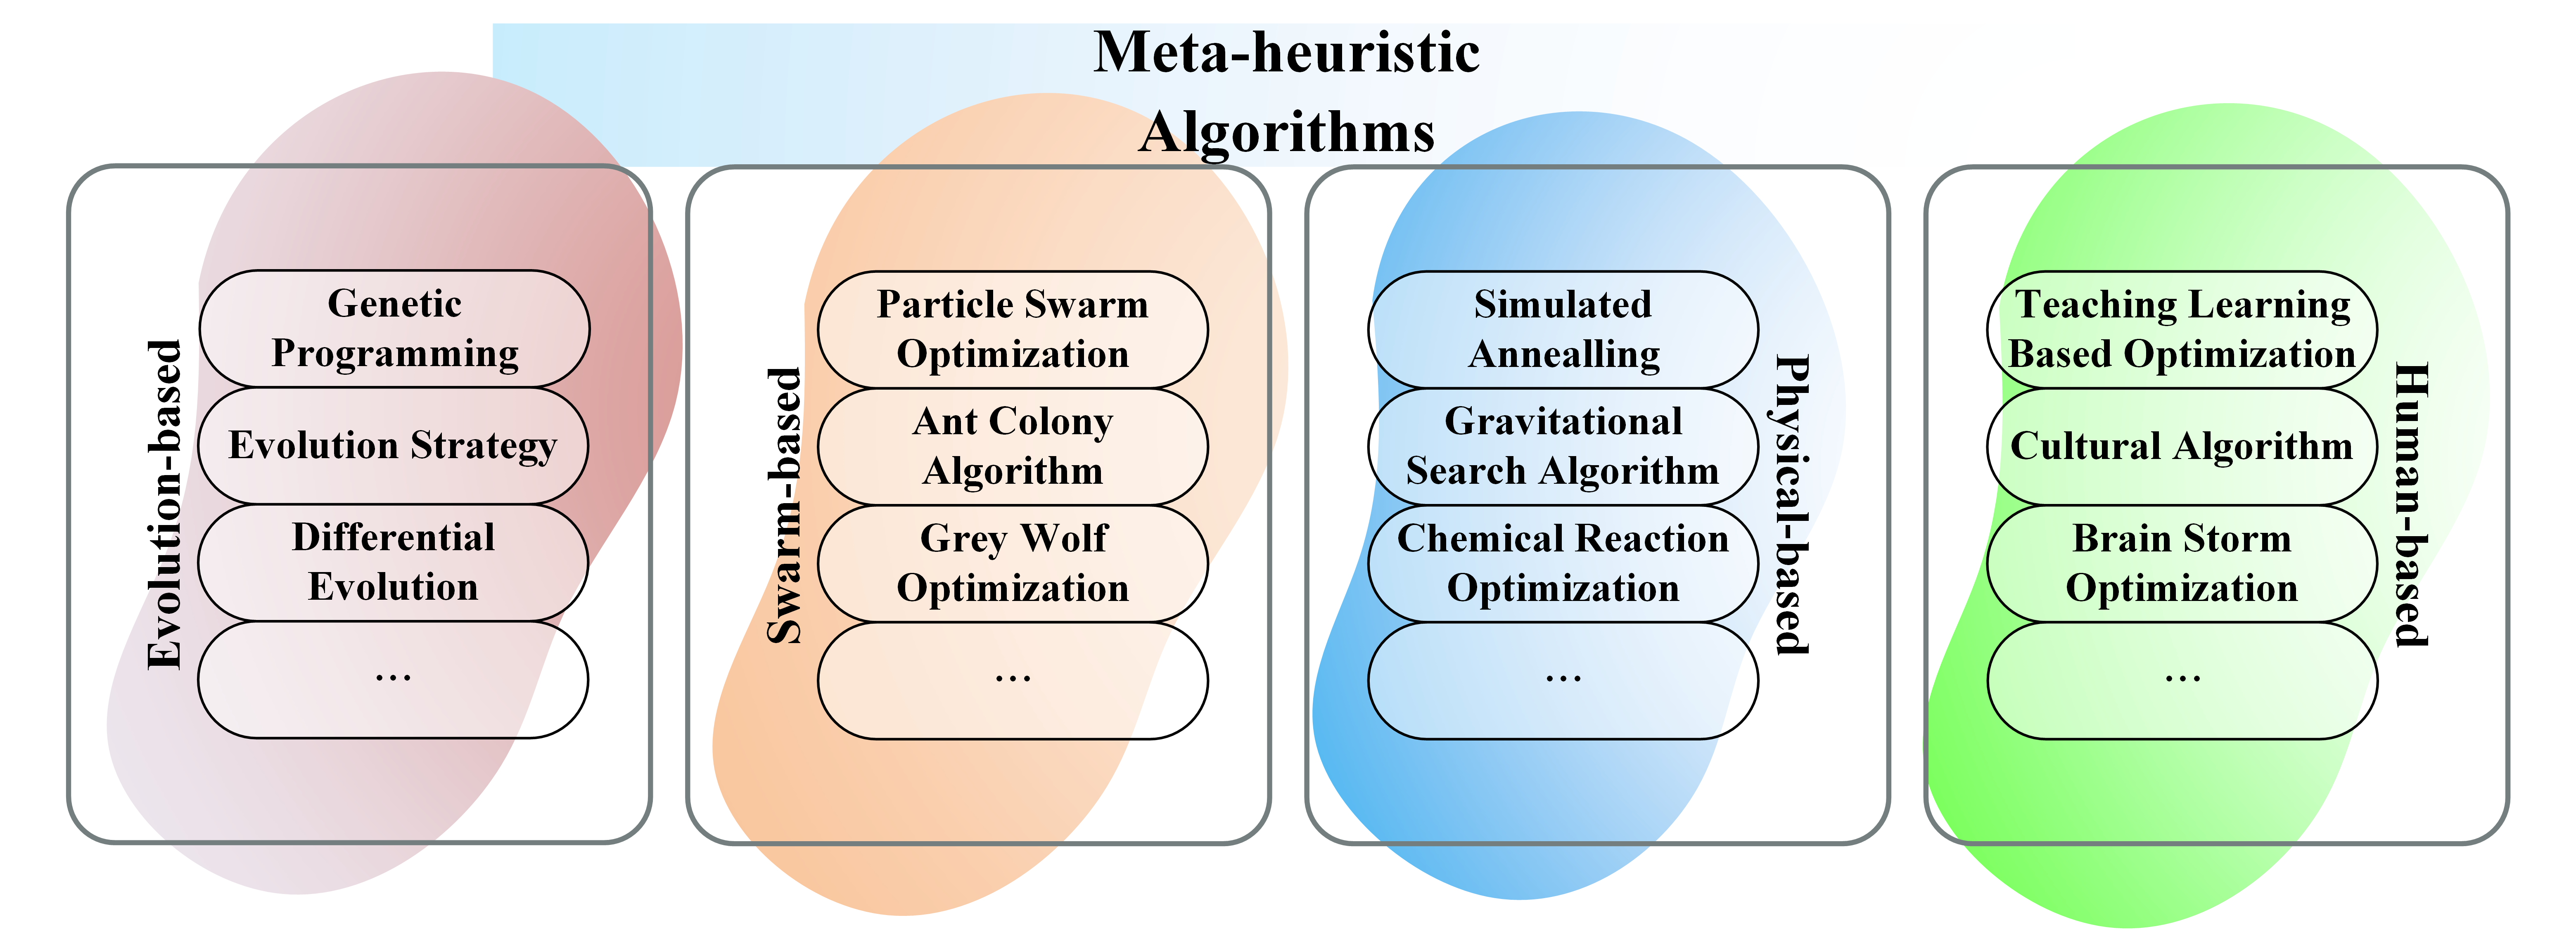
\includegraphics[width=\textwidth]{figures/fig01_classification_of_MAs.png}
  \caption{Four types of MAs.}
  \label{fig:classification_of_MAs}
\end{figure}

Considering the critical role of MAs in addressing modern optimization challenges, it is essential to explore their diverse forms, each employing unique, nature-inspired strategies to navigate complex problem landscapes. While MAs offer significant adaptability and robustness, they are commonly constrained by a substantial need for intricate parameter tuning. This requirement hinders scalability and real-world deployment, where optimal configurations are rarely static. Regardless of whether they are Evolutionary Algorithms (EAs) mimicking natural selection, Swarm Intelligence (SI) models replicating collective behavior, or even physics- and human-inspired heuristics, all these approaches face this fundamental constraint, thus raising questions about their practicality in dynamic environments.

Fig. 1 shows these four categories, each having distinct advantages and challenges, further showing the need for better optimization methods. In exploring this topic further, we will focus on how parameter tuning affects the balance between exploration and exploitation, aiming to enhance the effectiveness of MAs across diverse complex optimization scenarios. EAs play a key role within the range of MAs, using the principles of natural selection and survival of the fittest. Starting with the Genetic Algorithm (GA) [7], which copies genetic inheritance and mutation processes, the field of EAs has grown to include variations such as Genetic Programming (GP) [8], Evolutionary Strategies (ES) [9], and Differential Evolution (DE) [10]. EAs are known for their broad uses and ability to find global optima via an repeating selection process, crossover, and mutation [11]. Despite their strengths, EAs face a big problem: they are very sensitive to the tuning of settings, namely the mutation rate and crossover probability. The need to carefully adjust these parameters to suit different optimization environments has led to research into creating adaptive and self-tuning evolutionary algorithms [12, 13]. This focus seeks to make easier parameter calibration while also improving the flexibility of EAs in addressing a wide range of optimization problems.

SI algorithms use ideas from the collective and self-organizing behaviors observed among social organisms. Methods such as Particle Swarm Optimization (PSO) [14], Ant Colony Optimization (ACO) [15], and Grey Wolf Optimization (GWO) [16] show these principles. PSO models the dynamic interaction seen in bird flocking. On the other hand, ACO copies the path-finding behavior of ants, while GWO simulates the collaborative hunting tactics of grey wolves. In the GWO method, each wolf within the virtual pack updates its position based on the influence of the alpha, beta, and delta wolves, which stand for the first, second, and third best solutions obtained so far, respectively. Through repeated steps, the wolf pack moves closer to a potential optimum, showing how well it works of the GWO as an optimization technique [17]. Swarm intelligence algorithms operate on the principle that a population of simple agents, following basic interaction rules, can together show complex and globally effective behaviors capable of addressing complicated optimization problems [18]. By emulating social behaviors, these algorithms efficiently explore the problem space through a basis in cooperation and information exchange among all search agents. Despite their built-in flexibility and robust parallel search capabilities, these algorithms face challenges related to parameter configuration. Key settings, including the number of agents involved, the interaction rules, and the convergence criteria, play a key part in determining the algorithms' performance and convergence rates [19].

Physics/chemistry-inspired methods present a different way to optimization, using the processes and laws of physics and chemistry. This category includes algorithms like Simulated Annealing (SA) [20] and Gravitational Search Algorithm (GSA) [21]. The former is influenced by metallurgical annealing, and the latter based on the principles of gravity and mass interaction. Further, methods such as the Chemical Reaction Optimization (CRO) [22] simulate molecular interactions and energetic exchanges observed in chemical reactions. These algorithms are particularly commended for their ability to evade local optimum [23], achieved through emulating the adaptive and stochastic behaviors present in physical and chemical systems. Despite the innovative exploration strategies introduced by these algorithms, they continue to face challenges related to parameter selection [24], a key issue that influences the balance between exploration and exploitation, ultimately affecting their ability to identify good solutions.

Algorithms based on human behavior demonstrate how incorporating cognitive processes and societal interactions into meta-heuristic optimization frameworks. For instance, algorithms like Teaching-Learning-Based Optimization (TLBO) [25] model the dynamics of educational environments, the Cultural Algorithm (CA) [26] mirrors the evolution and transmission of cultural knowledge, and Brain Storm Optimization (BSO) [27] simulates the collective problem-solving power of brainstorming. These algorithms excel due to copying human-centric problem-solving tactics, which include learning from experience, utilizing memory, and the small effect of social interaction [28]. However, the performance of these algorithms relies heavily on how accurately they simulate complex human behaviors. A key issue lies in the adjustment of parameters governing individual learning and social dynamics, which can greatly affect the algorithms' skill in exploring the search spaces.

In our effort to improve the meta-heuristic methods, we propose the Status-based Optimization (SBO), an efficient algorithm that models the details of human status progression. The basis of SBO is deeply based on the seemingly invisible yet strong networks of social upward mobility, wherein individuals actively seek connections with and learn from their more skilled peers. The design of SBO shows this natural tendency to aspire towards excellence and gain useful knowledge and resources for self-improvement [29].

Similarly, climbing social ladders can lead to personal growth and enrichment, the SBO algorithm copies this progression within the optimization field. It shows the exploration phase as an individual's effort to enter a higher-status circle, which, in algorithmic terms, is like searching the most promising areas of the solution space. Following this, the exploitation phase is seen as the individual using the opportunities and connections gained within this advanced circle, like refining the best solutions for optimal performance. Therefore, the SBO algorithm makes a direct comparison between the continuous human effort to improve through engagement aimed at status enhancement and the systematic optimization method. It does this through its great flexibility and carefully designed framework. The main findings of this paper can be summed up as follows:

\begin{enumerate}
\item  The introduction of the SBO, a new MA that copies human status-seeking behaviors and interactions, provides a new way to heuristic optimization.

\item  Showing strong ability in global optimization, the performance of the SBO algorithm is validated through thorough tests using the IEEE CEC 2017 test suite.

\item  The reliability of the SBO algorithm's performance is validated through detailed stats tests, including the Wilcoxon signed-rank test and the Friedman test. These tests confirm the statistical significance and reliability of its optimization results.

\item  The usefulness and effectiveness of the SBO algorithm are further demonstrated in high-dimensional feature selection and multi-threshold image segmentation tasks. These results provide evidence of its potential flexibility and indicate its usefulness across various engineering domains.
\end{enumerate}

The structure of this paper is as follows: Section 2 reviews human behavior-inspired meta-heuristic algorithms, setting the base for the detailed look of the SBO in Section 3, which studies its conceptual basis and underlying mathematical model. Section 4 fully tests the SBO's performance against established benchmarks, while Section 5 demonstrates its use to real-world feature selection and multi-threshold image segmentation tasks. Finally, Section 6 summarizes main results and discusses potential future research directions.


\section{ Literature Review}

Optimization algorithms are divided into two main types: heuristic and meta-heuristic methods. Heuristic algorithms are specialized approaches that use pre-set rules or expert knowledge to find good-enough solutions quickly, though they cannot promise the best possible answer. They're custom-built for specific problems, like greedy algorithms and local search methods.

On the other hand, MAs are flexible problem-solvers that manage the search process to balance wide-ranging exploration and focused improvement. Unlike heuristics, meta-heuristics can tackle many different problems without major changes. They often use random elements and self-adjusting methods to escape local optima, making them better for tough, high-dimensional problems. It's worth noting that many meta-heuristic algorithms include heuristics as part of their solution-improving process, showing how the two types connect.

Our research places the new SBO algorithm in the meta-heuristic category, as it uses adaptive learning inspired by how people seek higher social status to improve search efficiency. Different from traditional heuristic methods that follow fixed rules, SBO changes its search strategy on the fly by sharing information and evaluating resources, boosting both exploration and exploitation. Because human behavior-inspired algorithms have made such an impact in research, we focus our review on key examples in this field. Particularly, TLBO, BSO, Political Optimization (PO), and Human Mental Search (HMS) stand out as strong examples of human-like problem-solving. Studying these not only helps position SBO within existing research but also shows how human-inspired strategies have developed in optimization field.

The TLBO [30] algorithm is one of the most classical human-inspired meta-heuristics, simulating a classroom's teaching--learning process without requiring algorithm-specific parameters. Its simplicity has led to various adaptations: for instance, the Multi-Objective TLBO (MOTLBO) [31] optimizes structural design by efficiently navigating trade-offs between weight and material strength, and the Improved TLBO (ITLBO) [32] has been successfully applied to electrical distribution systems. Further, the Self-adaptive Hybrid Self-learning based TLBO (SHSLTLBO) [33] enhances the basic algorithm by introducing adaptive learning strategies to focus the search on promising regions.

The Brain Storm Optimization (BSO) algorithm [34] mimics human brainstorming, generating diverse solutions through iterative idea exchange. Enhancements such as the Optima-Identified Framework amalgamated with BSO (OIF-BSO) [35] improve search direction via an optima-identification mechanism, while the Advanced Grid-based BSO (AGBSO) [36] employs alternative search patterns and grid-based operators to navigate uncertain landscapes better.

The Political Optimization (PO) [37] draws from the complexities of human political systems, using a multi-agent framework where competitive and cooperative interactions drive the search for optimal solutions. Its effectiveness is further improved in variants like the Improved PO (IPO) [38], which adds sophisticated political strategies to boost performances, and the Quantum Nelder-Mead PO (QNMPO) [39], which hybridizes quantum principles with political optimization to enhance performance in energy systems.

The Human Mental Search (HMS) algorithm [40] captures cognitive and decision-making processes inherent to human problem solving. The Global-Best Guided HMS with Random Clustering Strategy (GBG-HMS-RCS) [41] integrates global-best guidance with stochastic clustering to emulate human attention and awareness. Further, the Multi-Cluster Selection HMS (MCS-HMS) [42] forms multiple cognitive clusters to identify promising solution regions, a strategy that proves effective in complex scenarios such as supply chain management and transport logistics.

To summarize, this section has~carefully examined~an array of~important algorithms inspired by~different aspects~of human~behavior. The~teaching-learning~dynamics~shown~in TLBO, the~team-based creativity~in BSO, the~political strategies~in PO, and the~thought processes~in HMS all~turn human behavior~into computational~tools. While these human-inspired algorithms have~worked well~for complex problems, they also have~some weaknesses:

\begin{enumerate}
\item  TLBO~does not need parameters~but~can be slow to converge

\item  BSO~uses creative search methods~but~may converge too early

\item  PO~can require heavy computation

\item  HMS~often needs careful adjustment~for best results
\end{enumerate}

\noindent Compared to these, the new SBO algorithm offers~key improvements:

\begin{enumerate}
\item  Fewer settings to adjust, making it~easier to use

\item  Better balance~between~wide searching~and~local refining, thanks to its~social learning approach

\item  Faster runtimes, as shown in our tests (Section 4.4), where it~consistently beat~other methods
\end{enumerate}

\noindent These~benefits~make SBO~more useful~for~real-world~and~complex~optimization problems.

We developed SBO to combine the best features of these human-inspired approaches while overcoming their limitations. In the coming sections, we'll explain: What inspired SBO, how it works mathematically, and where it can be applied. This will show how SBO fits with other meta-heuristic methods and solves the problems found in current approaches.


\section{ Proposed Status-based Optimization}

This section focuses on the SBO algorithm's exposition, detailing its mathematical modeling and computational complexity.


\paragraph{ SBO Inspiration}

The SBO algorithm models humanity's essential drive to climb social ladders---a behavior rooted in our need for self-improvement [43]. This ambition mirrors optimization's core goal: iterative refinement. Like people gaining advantages by connecting with successful peers  [44], SBO agents learn from high-performing solutions to enhance search efficiency.

\noindent Research in cognitive science and behavioral economics confirms that learning from high-status individuals improves problem-solving in complex scenarios. SBO translates this into computational terms, creating a collective intelligence where:

\begin{enumerate}
\item  Agents share knowledge (like human networks)

\item  Diverse strategies emerge naturally

\item  The system balances exploration and exploitation
\end{enumerate}



In short, we can say this is how SBO works: 

\begin{enumerate}
\item  \textbf{Elite Engagement (Exploration)}

\begin{enumerate}
\item  Agents~follow top performers~to~discover promising regions

\item  Analogous to~seeking mentors~in social hierarchies
\end{enumerate}

\item  \textbf{Resource Phases (Exploitation)}

\begin{enumerate}
\item  \textbf{Acquisition}: Gather information from elites

\item  \textbf{Evaluation}: Refine solutions~like professionals improving skills
\end{enumerate}
\end{enumerate}



Several optimization algorithms inspired by human status-driven social behaviors and educational interactions have successfully solved complex problems. The Human Behavior-Based Optimization (HBBO) algorithm [45] mimics collective human behaviors such as cooperation, competition, imitation, and social learning. HBBO balances social learning with individual creativity through mechanisms like imitation, innovation, and collaboration, making it suitable for dynamic or multi-objective problems.

Similarly, the Educational Competition Optimizer (ECO) [46] models competitive learning environments where solutions compete and learn from top performers, guided by the best solution, akin to a teacher. This approach promotes rapid convergence and adaptability to constrained optimization scenarios, showcasing its efficiency in applications like academic performance modeling and game theory.



By formalizing status-seeking behaviors, SBO outperforms predecessors in:

\begin{enumerate}
\item  Balancing global/local search

\item  Reducing manual parameter tuning

\item  Scaling to high-dimensional problems
\end{enumerate}


\paragraph{ Mathematical Modeling of SBO}

Drawing inspiration from~human status-seeking behavior, the SBO algorithm~frames~optimization as~both~a personal and social development process. It begins by generating~two diverse populations of agents---representing individuals from different social backgrounds---who then evolve through~a process~modeled after~seeking mentorship from society's elite.

Key Phases are as follows:

\begin{enumerate}
\item  \textbf{Elite Pursuit}: Agents~identify and move toward~high-performing solutions (``mentors'')

\item  \textbf{Resource Acquisition}: They~gain~valuable information (social capital)

\item  \textbf{Strategic Integration}: Agents~critically evaluate and adopt~only the most beneficial improvements
\end{enumerate}

This mirrors how people:

\begin{enumerate}
\item  \textbf{Advance socially}~by learning from successful peers

\item  \textbf{Selectively adopt}~behaviors that enhance their status

\item  \textbf{Systematically climb}~hierarchies through accumulated advantages
\end{enumerate}

The algorithm culminates by~consolidating these improvements~to deliver~an optimal solution---mathematically representing~the pinnacle of status achievement. (Full mathematical details follow in later sections.)

\noindent 
\subparagraph{3.2.1 Initialization}

The Initialization phase lays the foundation of the SBO algorithm by generating two populations, $X^1$ and $X^2$. In this model, each index $i$ corresponds to a unique family, where the same-indexed individuals across $X^1$ and $X^2$ represent family members with distinct knowledge levels and social standings. This dual-population design ensures that each family is represented by at least two individuals, thereby capturing intra-family diversity and enabling dynamic updating of the elite member as the algorithm iterates.

\begin{tabular}{|p{0.4in}|p{3.1in}|p{0.4in}|} \hline 
 & $X^1,\ X^2={\left[ \begin{array}{c}
x_1 \\ 
\vdots  \\ 
x_2 \\ 
\vdots  \\ 
x_N \end{array}
\right]}_{N\times D}={\left[ \begin{array}{ccccc}
x_{1,1} & \cdots  & x_{1,j} & \cdots  & x_{1,N} \\ 
\vdots  & \ddots  & \vdots  & \ddots  & \vdots  \\ 
x_{i,1} & \cdots  & x_{i,j} & \cdots  & x_{i,D} \\ 
\vdots  & \ddots  & \vdots  & \ddots  & \vdots  \\ 
x_{N,1} & \cdots  & x_{N,j} & \cdots  & x_{N,D} \end{array}
\right]}_{N\times D}$ & $\left(\mathrm{1}\right)$ \\ \hline 
\end{tabular}



Each individual's state is defined by Eq. \left(\mathrm{2}\right):

\begin{tabular}{|p{0.4in}|p{3.1in}|p{0.4in}|} \hline 
 & $x_{i,j}=U\left(lb_j,\ ub_j\right)$ & $\left(\mathrm{2}\right)$ \\ \hline 
\end{tabular}

where $x_{i,j}$ is the $jth$ decision variable of the $ith$ individual, $D$ is the number of decision variables, and $lb_j$ and $ub_j$ are the lower and upper bounds, respectively. This uniform initialization across the $N\times D$ matrices for both populations establish the problem's dimensional nature and ensures a diverse starting point.

After initialization, a selection process identifies the elite member for each family to form the elite population $X^e$. Specifically, for the $ith$ family,

\begin{tabular}{|p{0.4in}|p{3.1in}|p{0.4in}|} \hline 
 & $ \begin{array}{c}
x^e_i=\left\{ \begin{array}{c}
x^1_i\ \ \ \ \ \ \ \ \ \ \ \ \ \ \ \ \ \ \ \ if\ fobj\left(x^1_i\right)<fobj\left(x^2_i\right)\ \ \ \ \ \ \ \ \ \ \ \ \ \ \ \ \ \ \  \\ 
x^2_i\ \ \ \ \ \ \ \ \ \ \ \ \ \ \ \ \ \ \ \ \ \ \ \ \ \ \ \ \ \ \ \ otherwise\ \ \ \ \ \ \ \ \ \ \ \ \ \ \ \ \ \ \ \ \ \ \ \ \ \ \ \ \ \ \ \ \ \  \end{array}
\right.\# \end{array}
$ & $\left(\mathrm{3}\right)$ \\ \hline 
\end{tabular}

where $fobj\left(\cdot \right)$ is the objective function.

This dual-population approach does more than just find top performers in each group---it mirrors real-world social mobility, where progress depends on both individual merit and strategic connections. The interactions between regular individuals $x_i$ and their elite counterparts $x^e_i$ simulate real-world status-oriented social networks, illustrating how elite figures facilitate progress and resource sharing within and across family units.

\noindent 
\subparagraph{3.2.2 Elite Engagement}

In the Elite Engagement phase, the SBO algorithm replicates the complex dynamics of human social status structures to enhance the search for optimal solutions. This phase models individuals seeking guidance from high-status mentors---elite agents in the algorithm---to expedite their progress. Unlike isolated family frameworks, this progression extends beyond self-contained groups by establishing interconnections between different social units, creating a more adaptive and robust search mechanism.

To emulate this behavior, the SBO algorithm uses the Roulette Wheel selection method [47] to choose an individual from a subset of the population. This subset represents the most successful members across different families. This probabilistic selection process ensures that individuals do not solely rely on a single dominant peer but instead consider multiple influential agents, reflecting the unpredictable yet strategic nature of human networking.

The selected individual, denoted as $x^e_r$, and the best individual in the population, $x_b$, together define a high-status circle---a metaphorical yet computationally significant region within the solution space that agents aim to integrate into. This dynamic representation of social mobility ensures that individuals systematically transition towards more promising areas of the search space.

To mathematically articulate this behavior, Eq. \left(\mathrm{4}\right) and Fig. 2 delineate the generation of individuals $x_i$ within the high-status circle---defining the area of promise within the solution space. This high-status circle represents an adaptive region where individuals navigate toward better solutions, balancing both structured progression and exploratory randomness. The movement of an individual is governed by:

\begin{tabular}{|p{0.2in}|p{3.5in}|p{0.2in}|} \hline 
 & $x_{i'}=\left\{ \begin{array}{cc}
\left(1-w_1-w_2\right)\times x_i+w_1\times x^e_r+w_2\times x_b & if\ rand<w_3 \\ 
w_4\times \left(\left(1-w_1-w_2\right)\times x_i+w_1\times x^e_r+w_2\times x_b\right) & Otherwise \end{array}
\right.$ & $\left(\mathrm{4}\right)$ \\ \hline 
\end{tabular}

where $x_i$ represents the $ith$ individual in the population, $x_{i'}$ denotes the next iteration, $x^e_r$ is an elite individual selected via the Roulette Wheel method from the $X^E$ population, and $x_b$ is the best solution found so far. The movement strategy in Eq. \left(\mathrm{4}\right) ensures that individuals are influenced by their own position, a high-performing peer, and the best-known solution.

The parameters $w_1$ and $w_2$ are generated using $randn$, providing normally distributed randomness to weight the contributions of $x_i$, $x^e_r$, and $x_b$. These values introduce stochasticity while ensuring the movement remains within a logical bound, fostering a controlled yet diverse search across the solution space.

In contrast, $w_3$ and $w_4$ are designed parameters that dynamically adjust the influence of the high-status circle on exploration and exploitation. $w_3$ is calculated as:

\begin{tabular}{|p{0.4in}|p{3.1in}|p{0.4in}|} \hline 
 & $ \begin{array}{c}
w_3={\mathrm{tanh} \left({\left(\frac{\sqrt{\left|MaxFEs-randn\times FEs\right|}}{i}\right)}^{\frac{FEs}{MaxFEs}}\right)\ }\# \end{array}
$ & $\left(\mathrm{5}\right)$ \\ \hline 
\end{tabular}

where $MaxFEs$ denotes the maximum number of function evaluations, $FEs$ is the current number of evaluations, and $i$ is the index of the individual. This formulation allows $w_3$ to adapt as optimization progresses, determining whether the standard update rule or a more randomized search should be applied.

If $rand\ge w_3$, the second formulation in Eq. \left(\mathrm{4}\right) is used, where $w_4$ serves as a scaling factor that generates a uniformly distributed random number between $[-w_3,w_3]$. This mechanism increases exploration diversity by enabling step-size adjustments, particularly when escaping local optima.

\begin{tabular}{|p{0.4in}|p{3.1in}|p{0.4in}|} \hline 
 & $w_4=unifrnd\left(-w_3,\ w_3\right)$ & $\left(\mathrm{6}\right)$ \\ \hline 
\end{tabular}



\begin{figure}[htbp]
  \centering
  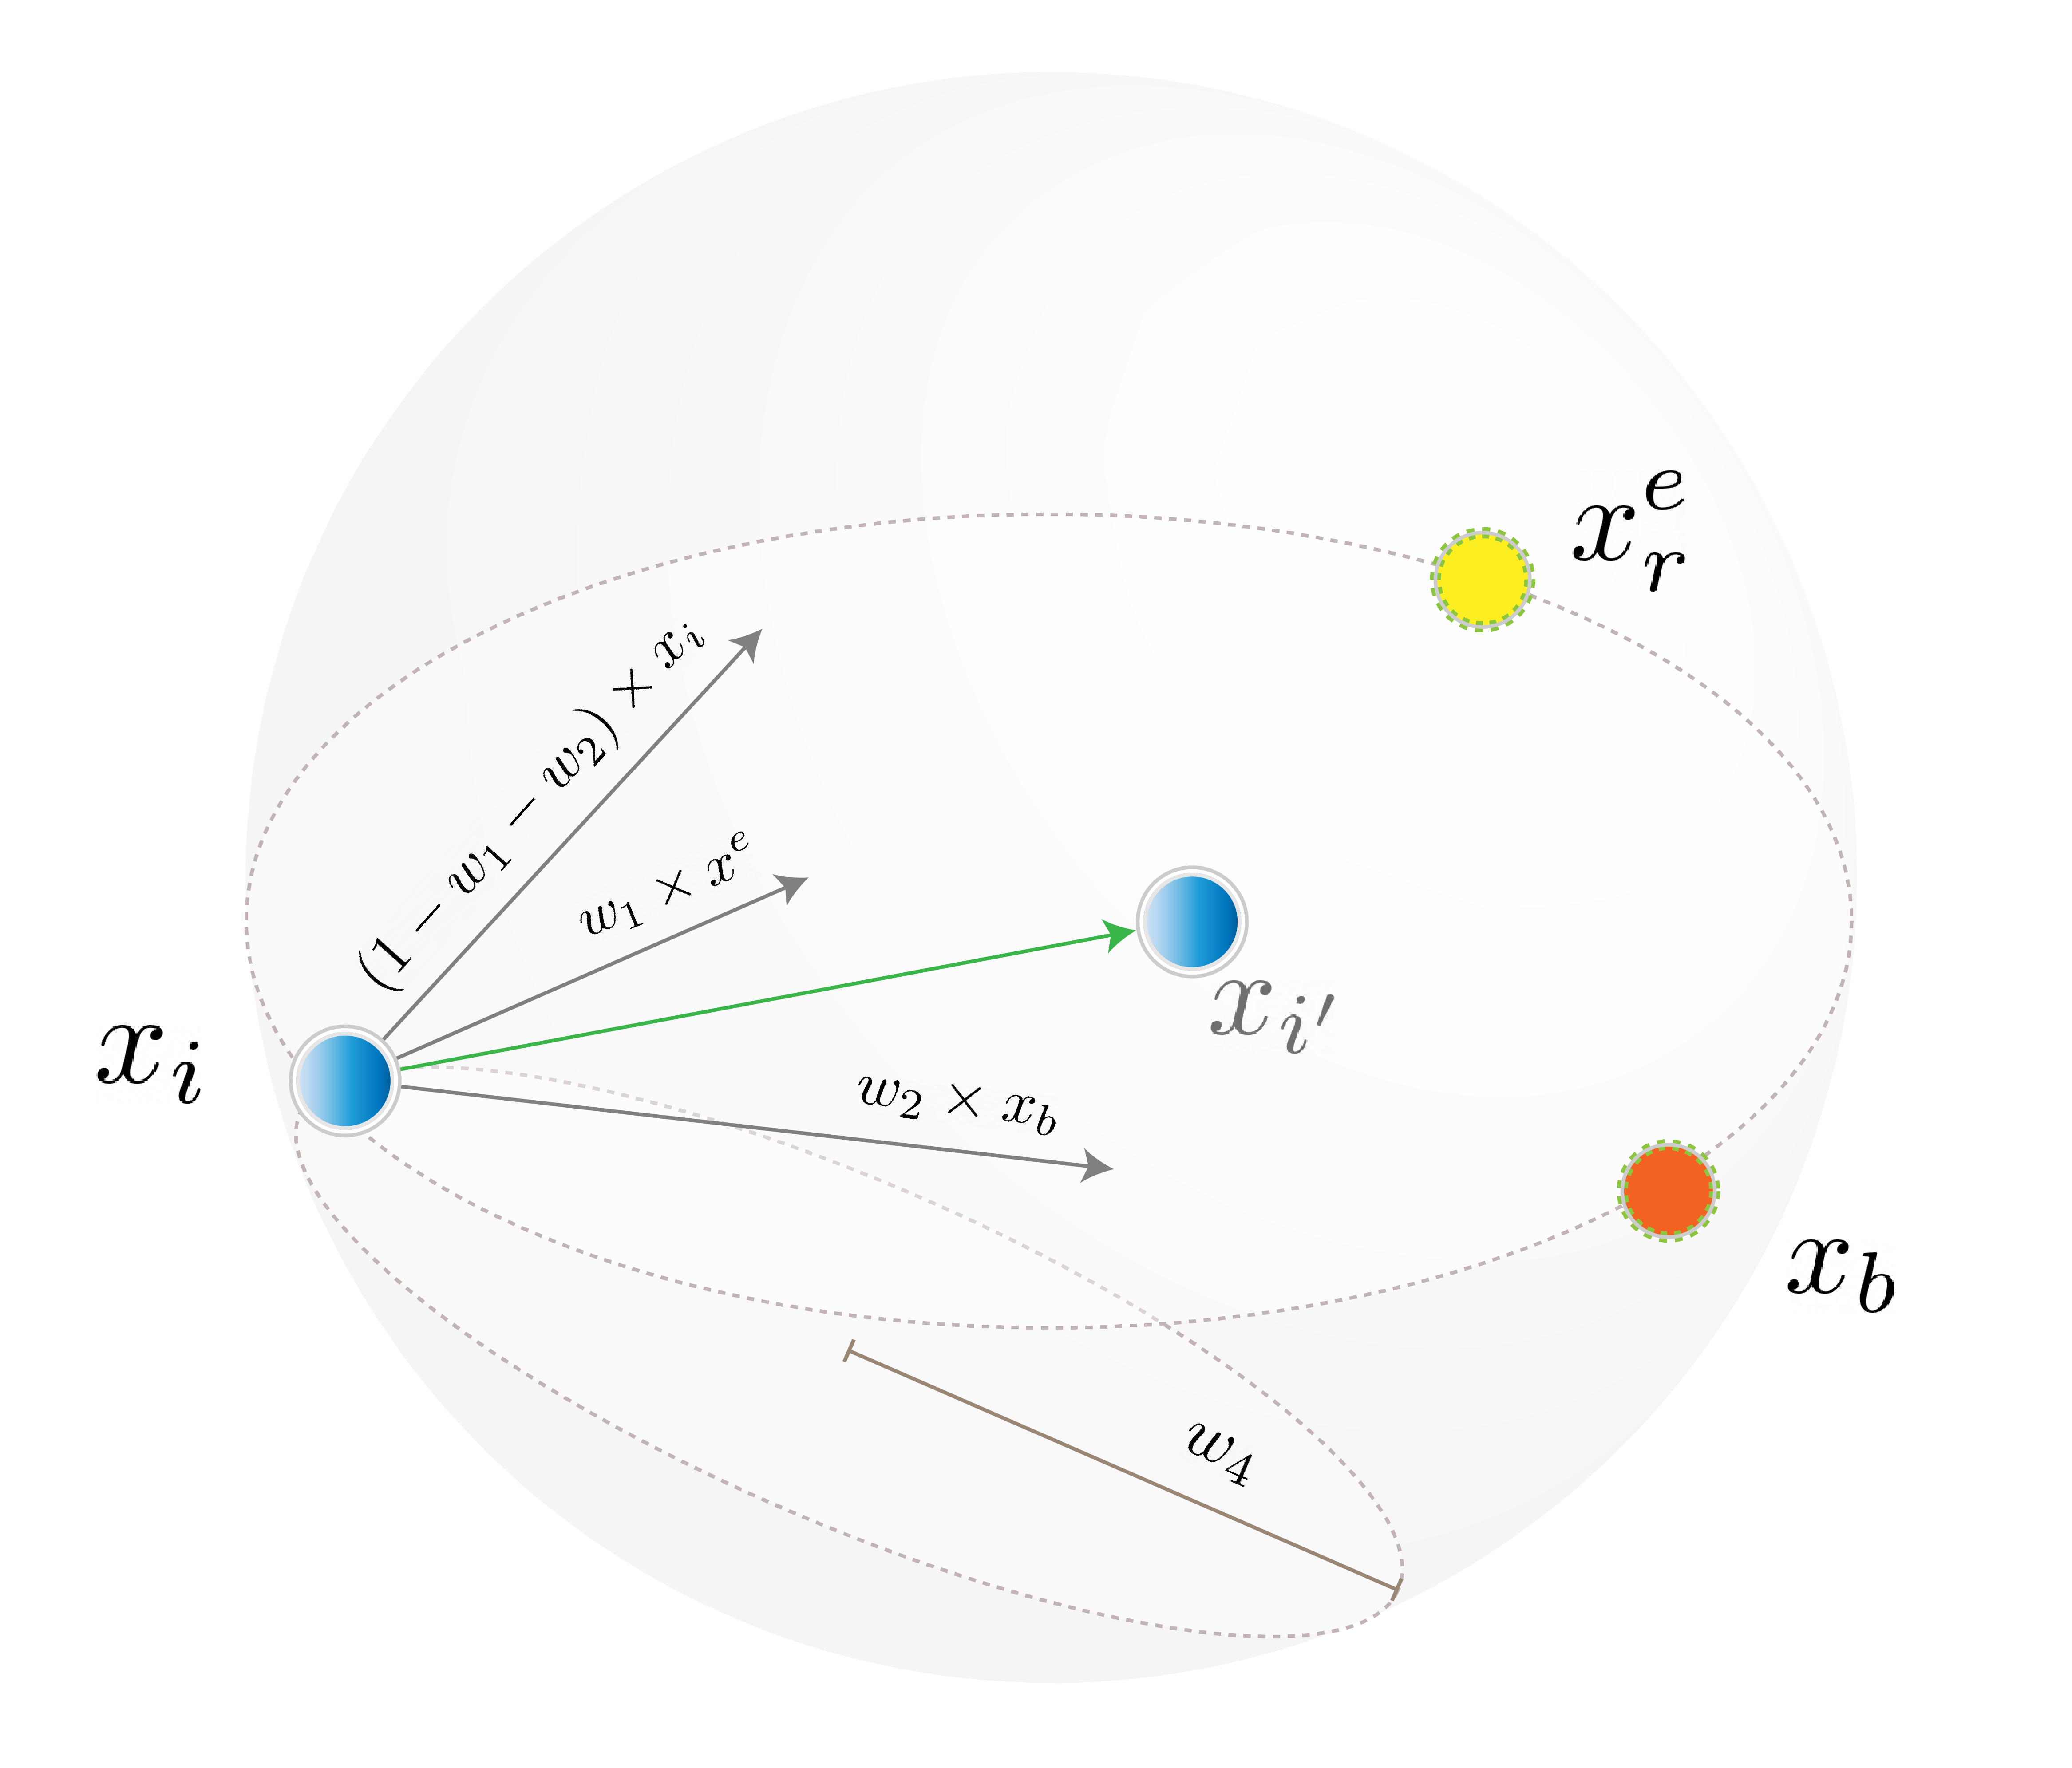
\includegraphics[width=\textwidth]{figures/fig02_elite_engagement.png}
  \caption{Elite Engagement phase of SBO.}
  \label{fig:elite_engagement}
\end{figure}



By integrating these components, the SBO algorithm mirrors real-world decision-making---where individuals pursue successful peers while strategically exploring unconventional paths to optimize outcomes. The initial formulation in Eq. \left(\mathrm{4}\right) strategically calculates an optimal position within the high-status circle, mirroring how individuals gain access to influential networks for better prospects. Through evolutionary computation, solutions progressively improve, moving toward more promising regions of the search space.

In contrast, the second formulation introduces a randomized scaling factor ranging from $[-w_3,w_3]$, allowing the algorithm to explore beyond the immediate promising area. This feature prevents premature convergence while enabling SBO to discover potentially superior solutions in unexplored areas. This balance reflects human decision-making. People sometimes diverge from established paths, whether through career changes or innovative ventures, to find opportunities missed by conventional approaches.

By combining structured learning and exploratory flexibility, SBO achieves an optimal balance between exploitation and exploration. This allows the algorithm to adapt effectively to complex optimization landscapes. The resulting approach improves solution quality while maintaining robustness across diverse problems, proving SBO's capability for high-performance optimization.

\noindent 
\subparagraph{3.2.3 Resource Acquisition}

The Resource Acquisition phase is crucial in transitioning from exploration to exploitation by acquiring and utilizing valuable insights---like social capital in human networks. In this phase, a $flag$ vector is created for all individuals in the $X$ population, initially set to 1 to indicate tentative status-related success. This flag later updates during the Resource Evaluation phase, serving as a dynamic indicator of each individual's efficacy in status improvement.

The resource acquisition mechanism varies based on status-related success. For socially successful individuals, resources are acquired selectively by averaging inputs from two sources: one from the elite individual within the same family unit and another from the overall best individual in the population. This process, captured by

\begin{tabular}{|p{0.4in}|p{3.1in}|p{0.4in}|} \hline 
 & $x^s_{i,j_1}=\frac{x^e_{i,j_2}+x_{b,j_3}}{2}$ & $\left(\mathrm{7}\right)$ \\ \hline 
\end{tabular}

with $j_{idx}=randi\left(D\right)$ for $idx=1,2,3$, reflects the blend of familial and external elite influences.

Conversely, socially unsuccessful individuals rely solely on familial resources. Their resource update follows

\begin{tabular}{|p{0.4in}|p{3.1in}|p{0.4in}|} \hline 
 & $ \begin{array}{cc}
x^s_{i,j}=x^e_{i,j} & if\ m_j=1 \end{array}
$ & $\left(\mathrm{8}\right)$ \\ \hline 
\end{tabular}

where the row vector $m$ is initially zero and updated prior to social interactions by

\begin{tabular}{|p{0.4in}|p{3.1in}|p{0.4in}|} \hline 
 & $m\left(u\left(1:ceil\left(rand\times D\right)\right)\right)=1$ & $\left(\mathrm{9}\right)$ \\ \hline 
\end{tabular}

where $u=randperm(D)$ providing a random permutation of decision variable indices.

As shown in~Fig. 3, this phase~directs~the population toward promising regions of the solution space~to maximize~exploitation.

\begin{enumerate}
\item  Fig. 3(a)\textbf{:}~Successful individuals~refine~their positions by~using~resources from higher-status agents

\item  Fig. 3(b)\textbf{:}~Struggling individuals~reposition~themselves through familiar resource 
\end{enumerate}

\noindent 

The algorithm replicates status-driven social dynamics, where resource-rich individuals naturally attract more opportunities, to systematically guide the population toward better solutions, thereby significantly boosting exploitation and enhancing overall optimization performance.



\begin{figure}[htbp]
  \centering
  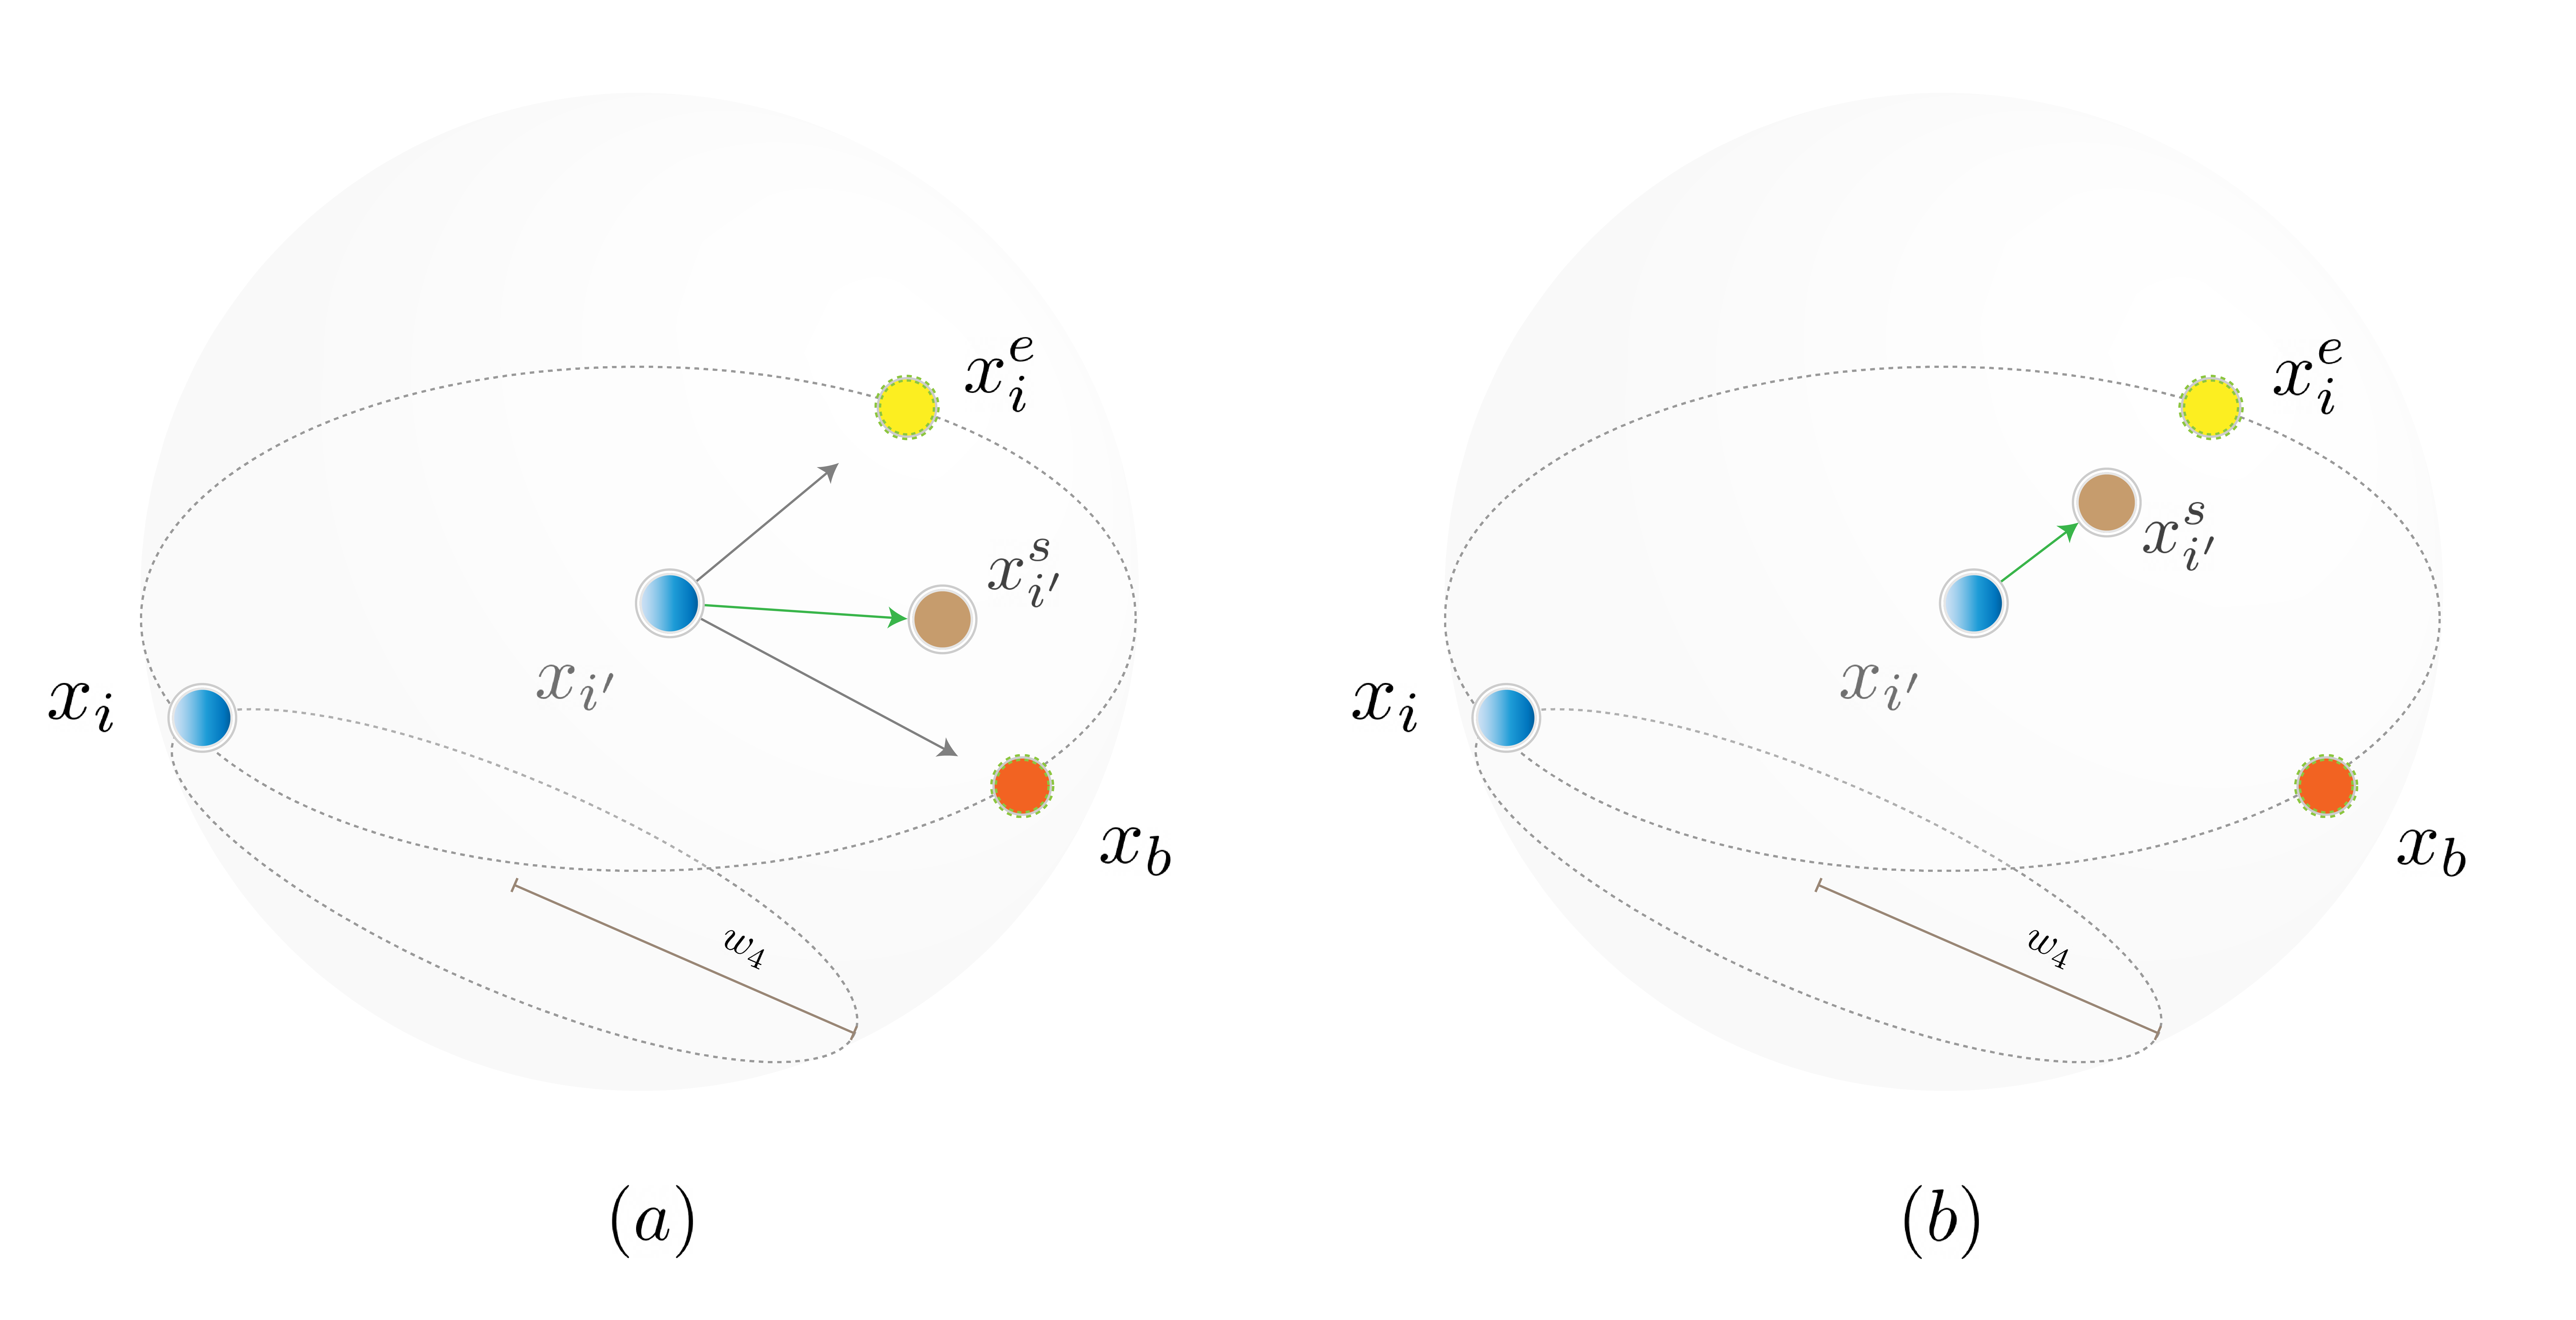
\includegraphics[width=\textwidth]{figures/fig03_resource_acquisition.png}
  \caption{Resource Acquisition phase of SBO.}
  \label{fig:resource_acquisition}
\end{figure}


\subparagraph{3.2.4 Resource Evaluation}

During the Resource Evaluation phase, the algorithm assesses whether acquired resources enhance an individual's fitness. Using the flag vector established earlier, it tracks progress:

\begin{enumerate}
\item  1 = Fitness improvement (success)

\item  0 = No improvement (failure)
\end{enumerate}



In practice, if the objective function value of the updated individual $x^s_i$ is better than that of the original $x_i$, the new state is retained:

\begin{tabular}{|p{0.4in}|p{3.1in}|p{0.4in}|} \hline 
 & $ \begin{array}{cc}
x_i=x^s_i & if\ fobj\left(x^s_i\right)<fobj\left(x_i\right) \end{array}
$ & $\left(\mathrm{10}\right)$ \\ \hline 
\end{tabular}

Simultaneously, the flag vector is refreshed as follows:

\begin{tabular}{|p{0.4in}|p{3.1in}|p{0.4in}|} \hline 
 & $flag_i=\left\{ \begin{array}{cc}
1 & if\ fobj\left(x^s_i\right)<fobj\left(x_i\right) \\ 
0 & Otherwise \end{array}
\right.$ & $\left(\mathrm{11}\right)$ \\ \hline 
\end{tabular}

Individuals showing no improvement maintain their current positions, while successful ones relocate to superior locations. This selective process mirrors real-world social advancement, where only valuable resources, those demonstrably improving an agent's status, are retained. This refinement progressively steers the search toward optimal solutions.

\noindent 
\subparagraph{3.2.5 Consolidation}

The Consolidation phase activates when termination criteria are met, either after reaching maximum function evaluations or achieving a sufficiently optimized solution (verified by enhancement metrics). Prior to this, the algorithm repeatedly cycles through its core phases:

\begin{enumerate}
\item  \textbf{Elite Engagement}

\item \textbf{ Resource Acquisition}

\item \textbf{ Resource Evaluation}
\end{enumerate}



Each phase~simulates status-driven interactions to~progressively improve~solutions.

\textbf{Implementation Details}:

\begin{enumerate}
\item  \textbf{Algorithm 1}~provides pseudo-code

\item  \textbf{Fig. 4}~shows the workflow
\end{enumerate}

\noindent \textbf{}

During Consolidation, the algorithm:~

\begin{enumerate}
\item  \textbf{Compiles and assesses}~results against objectives

\item  \textbf{Produces}~a final solution~embodying~status-based heuristics

\item  \textbf{Ensures}~efficient resource use~and~detailed documentation~for~analysis/application
\end{enumerate}



\begin{tabular}{|p{3.9in}|} \hline 
\textbf{Algorithm }1 Pseudo-code for the Status-based Optimization \\ \hline 
Input $N,\ D,\ MaxFEs,\ lb,\ ub,\ fobj$;\textit{} \\ \hline 
Initialization: \\ \hline 
    Initialize \textit{X}$,\ {\ X}^e,\ Fit,\ Fit^e,\ flag$; \\ \hline 
    Calculate $Fit$ and $Fit^e$; \\ \hline 
    Update $X^e$ and $x_b$; \\ \hline 
\textbf{While} $FEs\ <\ MaxFEs$ \\ \hline 
    Select $x^e_r$ from $X^e$ by Rolette Wheel; \\ \hline 
    Elite Engagement: \\ \hline 
        Update $w_1,\ w_2,\ w_3,\ and\ w_4$; \\ \hline 
        Update $X$ by Eq. \left(\mathrm{4}\right); \\ \hline 
        Apply Boundary control to $X$; \\ \hline 
        Initialize $X^s$ as $X$; \\ \hline 
    Resource Acquisition: \\ \hline 
        Initialize row vector $m$ as 0; \\ \hline 
        Update $m$ by Eq. \left(\mathrm{9}\right);\newline         \textbf{For} each $x^s$ in $X^s$:\newline             \textbf{If} $x^s$ is successful: \\ \hline 
                Update $x^s$ by Eq. \left(\mathrm{7}\right); \\ \hline 
            \textbf{Else}:\textbf{} \\ \hline 
                Update $x^s$ by Eq. \left(\mathrm{8}\right);\newline        \textbf{ End For} \\ \hline 
    Resource Evaluation:\textbf{} \\ \hline 
        Update $X$ by Eq. \left(\mathrm{10}\right); \\ \hline 
        Update $flag$ by Eq. \left(\mathrm{11}\right); \\ \hline 
    Consolidation: \\ \hline 
\textbf{        }Update $X^e$ and $x_b$;\textit{} \\ \hline 
\textbf{        }Increment\textbf{ }$FEs=FEs+2N$; \\ \hline 
\textbf{End While} \\ \hline 
\textbf{Return} $x_b$. \\ \hline 
\end{tabular}



\begin{figure}[htbp]
  \centering
  
\includegraphics[width=\textwidth]{figures/fig04_flowchart_SBO.png}
  \caption{Flowchart of SBO.}
  \label{fig:flowchart_SBO}
\end{figure}




\paragraph{ Computational Complexity Analysis of SBO}

The computational complexity of the SBO algorithm is primarily determined by the population size ($N$), the problem dimension ($D$), and the maximum number of iterations ($T$), which collectively define its termination criterion. In this analysis, we focus on the algorithm's most computationally demanding operations while omitting less impactful vector updates. The Initialization phase, involving the generation of two populations of size $N\times D$, requires $O(2ND)$ time. The Elite Engagement phase updates the solution in $O(ND)$ per iteration, culminating in a total complexity of $O(TND)$ over $T$ iterations. Both the Resource Acquisition and Resource Evaluation phases operate in $O(N)$ time per iteration, contributing $O(TN)$ cumulatively, while the Consolidation phase, which entails sorting, adds $O(TNlogN)$ to the overall cost. Summing these contributions, the total computational complexity of SBO is expressed as $O(TND+TN+TNlogN)$, a formulation that encapsulates the sequential and interdependent nature of its core operations. This analysis provides a concise quantitative estimate of the algorithm's efficiency and scalability in addressing a range of optimization challenges.


\section{ Performance Evaluation of SBO}

The sections below furnish an in-depth quality evaluation of the proposed SBO algorithm through a benchmark comparison involving 13 state-of-the-art algorithms and the 29 functions outlined by IEEE CEC 2017 [48]. These benchmark functions were carefully selected for their diversity and comprehensiveness---they include unimodal, multimodal, hybrid, and composition functions that collectively encapsulate a wide range of optimization challenges encountered in real-world problems. This rigorous benchmark suite, widely recognized and utilized in the optimization community, offers a robust framework for assessing the unique features of SBO, such as the balance and diversity in its search dynamics and the patterns of agent trajectories observed through detailed examination.

Performance metrics for this comparison are based on 30 independent runs per function, with average fitness values (Avg) and standard deviations (Std) serving as the primary indicators of algorithmic competence. All experiments were conducted in a controlled environment to ensure fairness and reproducibility. 

Specifically, all algorithms were evaluated on a Windows Server 2016 platform equipped with an Intel{\circledR} Xeon{\circledR} Silver 4210R CPU and 128 GB of RAM, using a population size of 30 and a maximum of 300,000 objective evaluations per run. The MATLAB R2018a ecosystem provided a reliable and standardized computational backbone for this extensive comparative study.


\paragraph{ Quality Analysis of SBO}

This section evaluates SBO's ability to balance exploration and exploitation---key aspects for an effective metaheuristic. We assess its capacity to shift from a broad global search to a focused local refinement while managing population diversity, as revealed by the historical distribution and trajectories of its search agents. This analysis highlights the interplay between diversification and convergence, offering insights into SBO's efficiency in navigating complex solution landscapes.

To quantify this balance, we use metrics that measure exploration (the search for new areas, which increases diversity) and exploitation (refining known good solutions, which decreases diversity). A practical algorithm typically exhibits strong early exploration, followed by intensified exploitation. We employ a dimension-wise diversity measure [49]:

\begin{tabular}{|p{0.4in}|p{3.1in}|p{0.4in}|} \hline 
 & $Div=\frac{1}{D}\int^D_{j=1}{Div_j}$ & $\left(\mathrm{12}\right)$ \\ \hline 
 & $Div_j=\frac{1}{N}\int^N_{i=1}{\left|X^j_i-mean\left(X^j\right)\right|}$ & $\left(\mathrm{13}\right)$ \\ \hline 
 & $mean\left(X^j\right)=\frac{1}{N}\int^N_{i=1}{X^j_i}$ & $\left(\mathrm{14}\right)$ \\ \hline 
\end{tabular}

where, $Div_j$ is the diversity in the $jth$ dimension, $D$ is the problem dimension, and $X^j_i$ is the $jth$ coordinate of the $ith$ solution. Based on this, we define the exploration and exploitation rates as follows:

\begin{tabular}{|p{0.4in}|p{3.1in}|p{0.4in}|} \hline 
 & $Exploration=\frac{Div\left(t\right)}{Div_{max}}\times 100\%$ & $\left(\mathrm{15}\right)$ \\ \hline 
 & $Exploitation=\frac{\left|Div\left(t\right)-Div_{max}\right|}{Div_{max}}\times 100\%$ & $\left(\mathrm{16}\right)$ \\ \hline 
\end{tabular}

where $Div(t)$ is the diversity at iteration $t$ and $Div_{max}$ is the maximum diversity observed.

For our experiments, we set the population size $N=30$, problem dimension $D=30$, and allow up to 300,000 evaluations. Fig. 5 displays the exploration rate, exploitation rate, population diversity, and convergence curves for eight functions from the IEEE CEC 2017 suite.

The functions selected for analysis span all four categories of the IEEE CEC 2017 suite. Specifically, we consider the unimodal function F1, multimodal functions F3 and F9, hybrid functions F11, F13, F16, and F19, and the composition function F26. Their three-dimensional distributions are illustrated in Fig. 5(a). Unimodal functions, with a single global optimum, primarily test an algorithm's convergence and exploratory efficiency. In contrast, multimodal functions assess the ability to escape local optima, while hybrid and composition functions, formed through combinations, rotations, and shifts, challenge the algorithm to balance exploration and exploitation effectively.

Fig. 5(b) demonstrates that SBO exhibits high exploration in the early iterations, transitioning to dominant exploitation in later stages. The incremental--decremental trend in the balance curve reflects this shift: an initial rise indicates vigorous global exploration, whereas the subsequent decline points to focused local exploitation. For example, with F1, the exploitation rate reaches 93.9\%, highlighting SBO's proficiency in refining toward the optimal solution.

Further, Fig. 5(b) and Fig. 5(c) reveal that SBO's population diversity steadily decreases before stabilizing, signifying ongoing improvements in solution quality. Multimodal functions F3 and F9 exhibit a similar pattern to F1, albeit with a slightly higher exploration rate due to their complexity. In the case of hybrid functions, a noticeable increase in the exploration rate, which peaks at 23.3\% for F13, coupled with marked fluctuations in diversity results in slower convergence compared to unimodal and multimodal cases. Nevertheless, the convergence curves in Fig. 5(d) confirm that SBO effectively avoids local optima by progressively refining solutions. For the composition function F26, an exploration rate of 12.7\% and a gradual decline in diversity underscore SBO's adept balance between global exploration and local exploitation, characterized by an initial surge in exploratory activity followed by a focused refinement phase.

\begin{figure}[htbp]
  \centering
  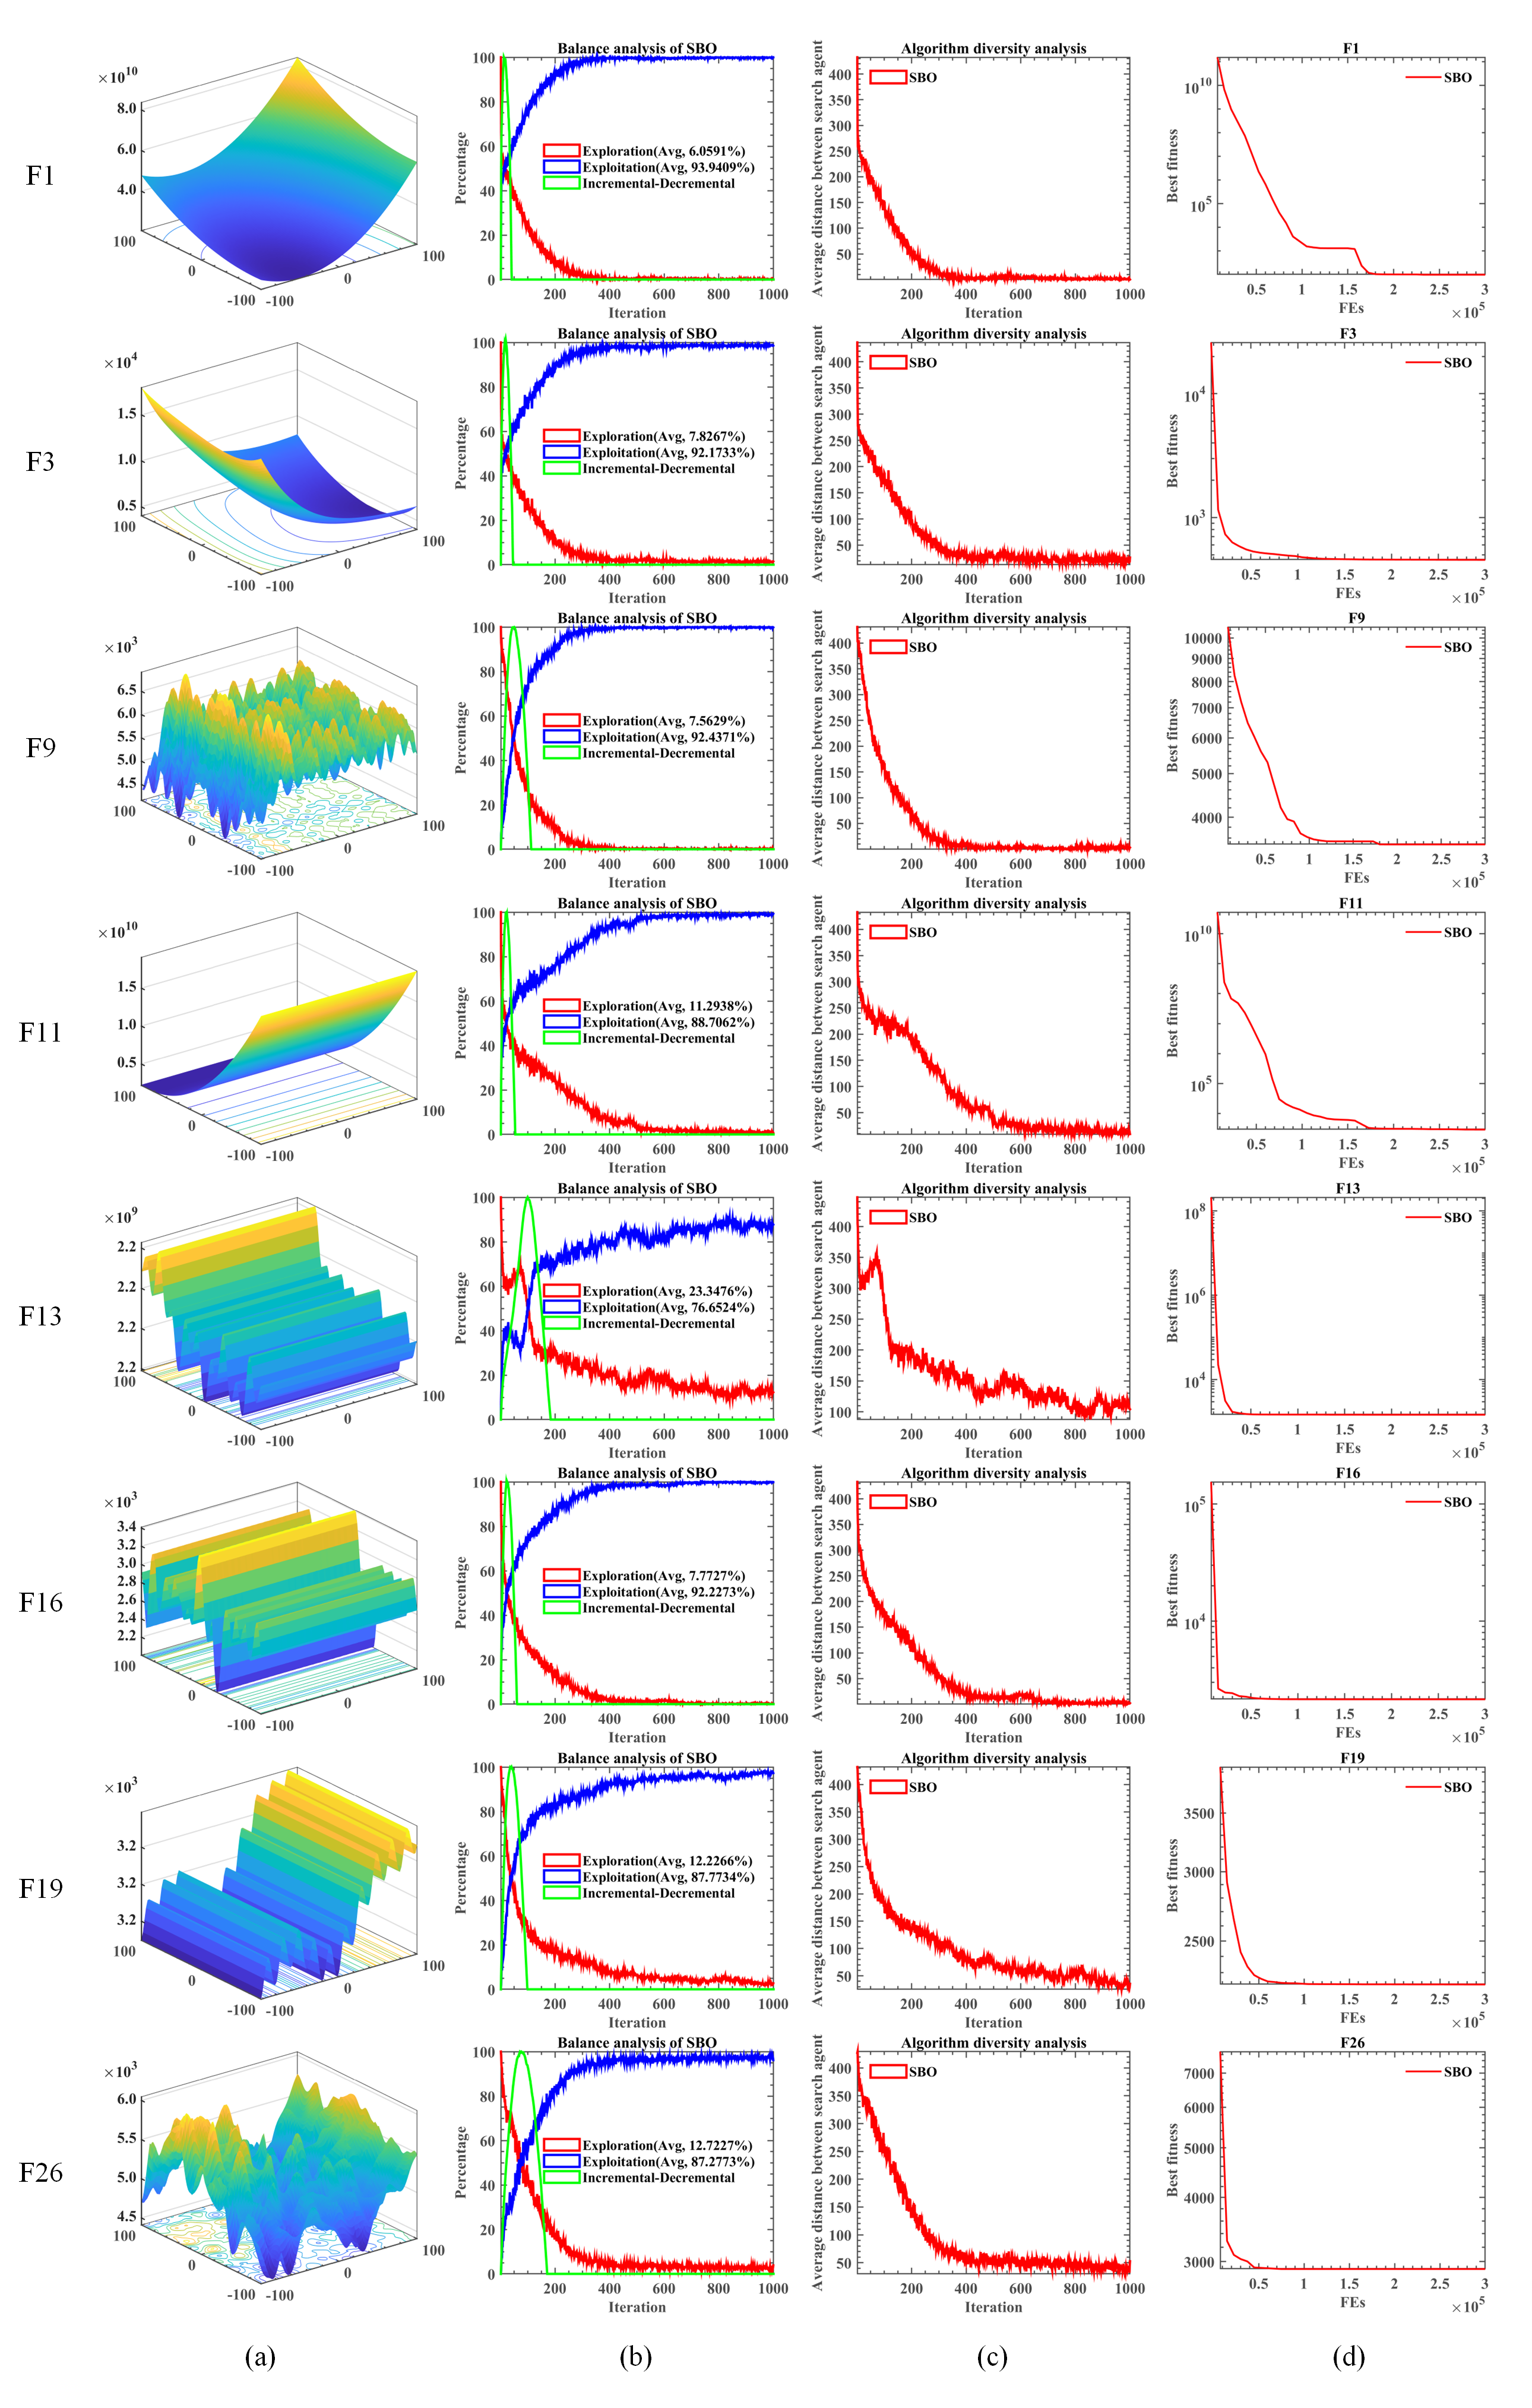
\includegraphics[width=\textwidth]{figures/fig05_balance_diversity_convergence.png}
  \caption{(a) 3D plots of functions, (b) balance analysis of SBO, (c) diversity analysis of SBO, (d) convergence curves of SBO.}
  \label{fig:balance_diversity_convergence}
\end{figure}



To investigate the SBO algorithm, we employed four evaluative metrics over 200 iterations with a constant population size of 30. These metrics enable a comprehensive qualitative assessment of the algorithm's behavior and effectiveness. In particular, the search history of the agents was recorded from the first to the last iteration, providing insights into the algorithm's explorative and exploitative movements throughout the search space. In addition, the trajectory of the best search agent, as indicated by variations in the first-dimensional variable over successive generations, was analyzed to illustrate the progression from initial exploration to subsequent exploitation. The average fitness of the search agents was computed over the entire evolutionary process to capture the algorithm's overall improvement. In contrast, the convergence curve, defined by the best fitness value attained by the population over time, offered a visual representation of the refinement process leading to the optimal solution.

These metrics were applied to eight functions selected from a set of 23 classical benchmark functions, with their three-dimensional representations depicted in Fig. 6(a). Fig. 6(b) presents the search history of the SBO algorithm's agents, where the optimal solutions are marked by red dots and the individual agents by black dots. The widespread dispersion of agents throughout the search space, coupled with a noticeable clustering near the optimum, underscores the algorithm's robust exploration capabilities and its effective local exploitation. This duality in behavior is attributed to distinct strategic phases inherent in SBO, wherein the exploration is predominantly reinforced during the Elite Engagement phase, and the exploitation is boosted through resource allocation among the most promising individuals.

Further analysis is provided by Fig. 6(c), which charts the trajectory of the best search agent's first-dimensional variable. The initial iterations exhibit significant fluctuations that eventually stabilize, reflecting the algorithm's transition from a phase of vigorous exploration to one of focused exploitation. Similarly, Fig. 6(d) illustrates that the average fitness of the agents begins at a higher level and either stabilizes or fluctuates within a narrow range as the process progresses, indicating a gradual convergence toward optimality.

\begin{figure}[htbp]
  \centering
  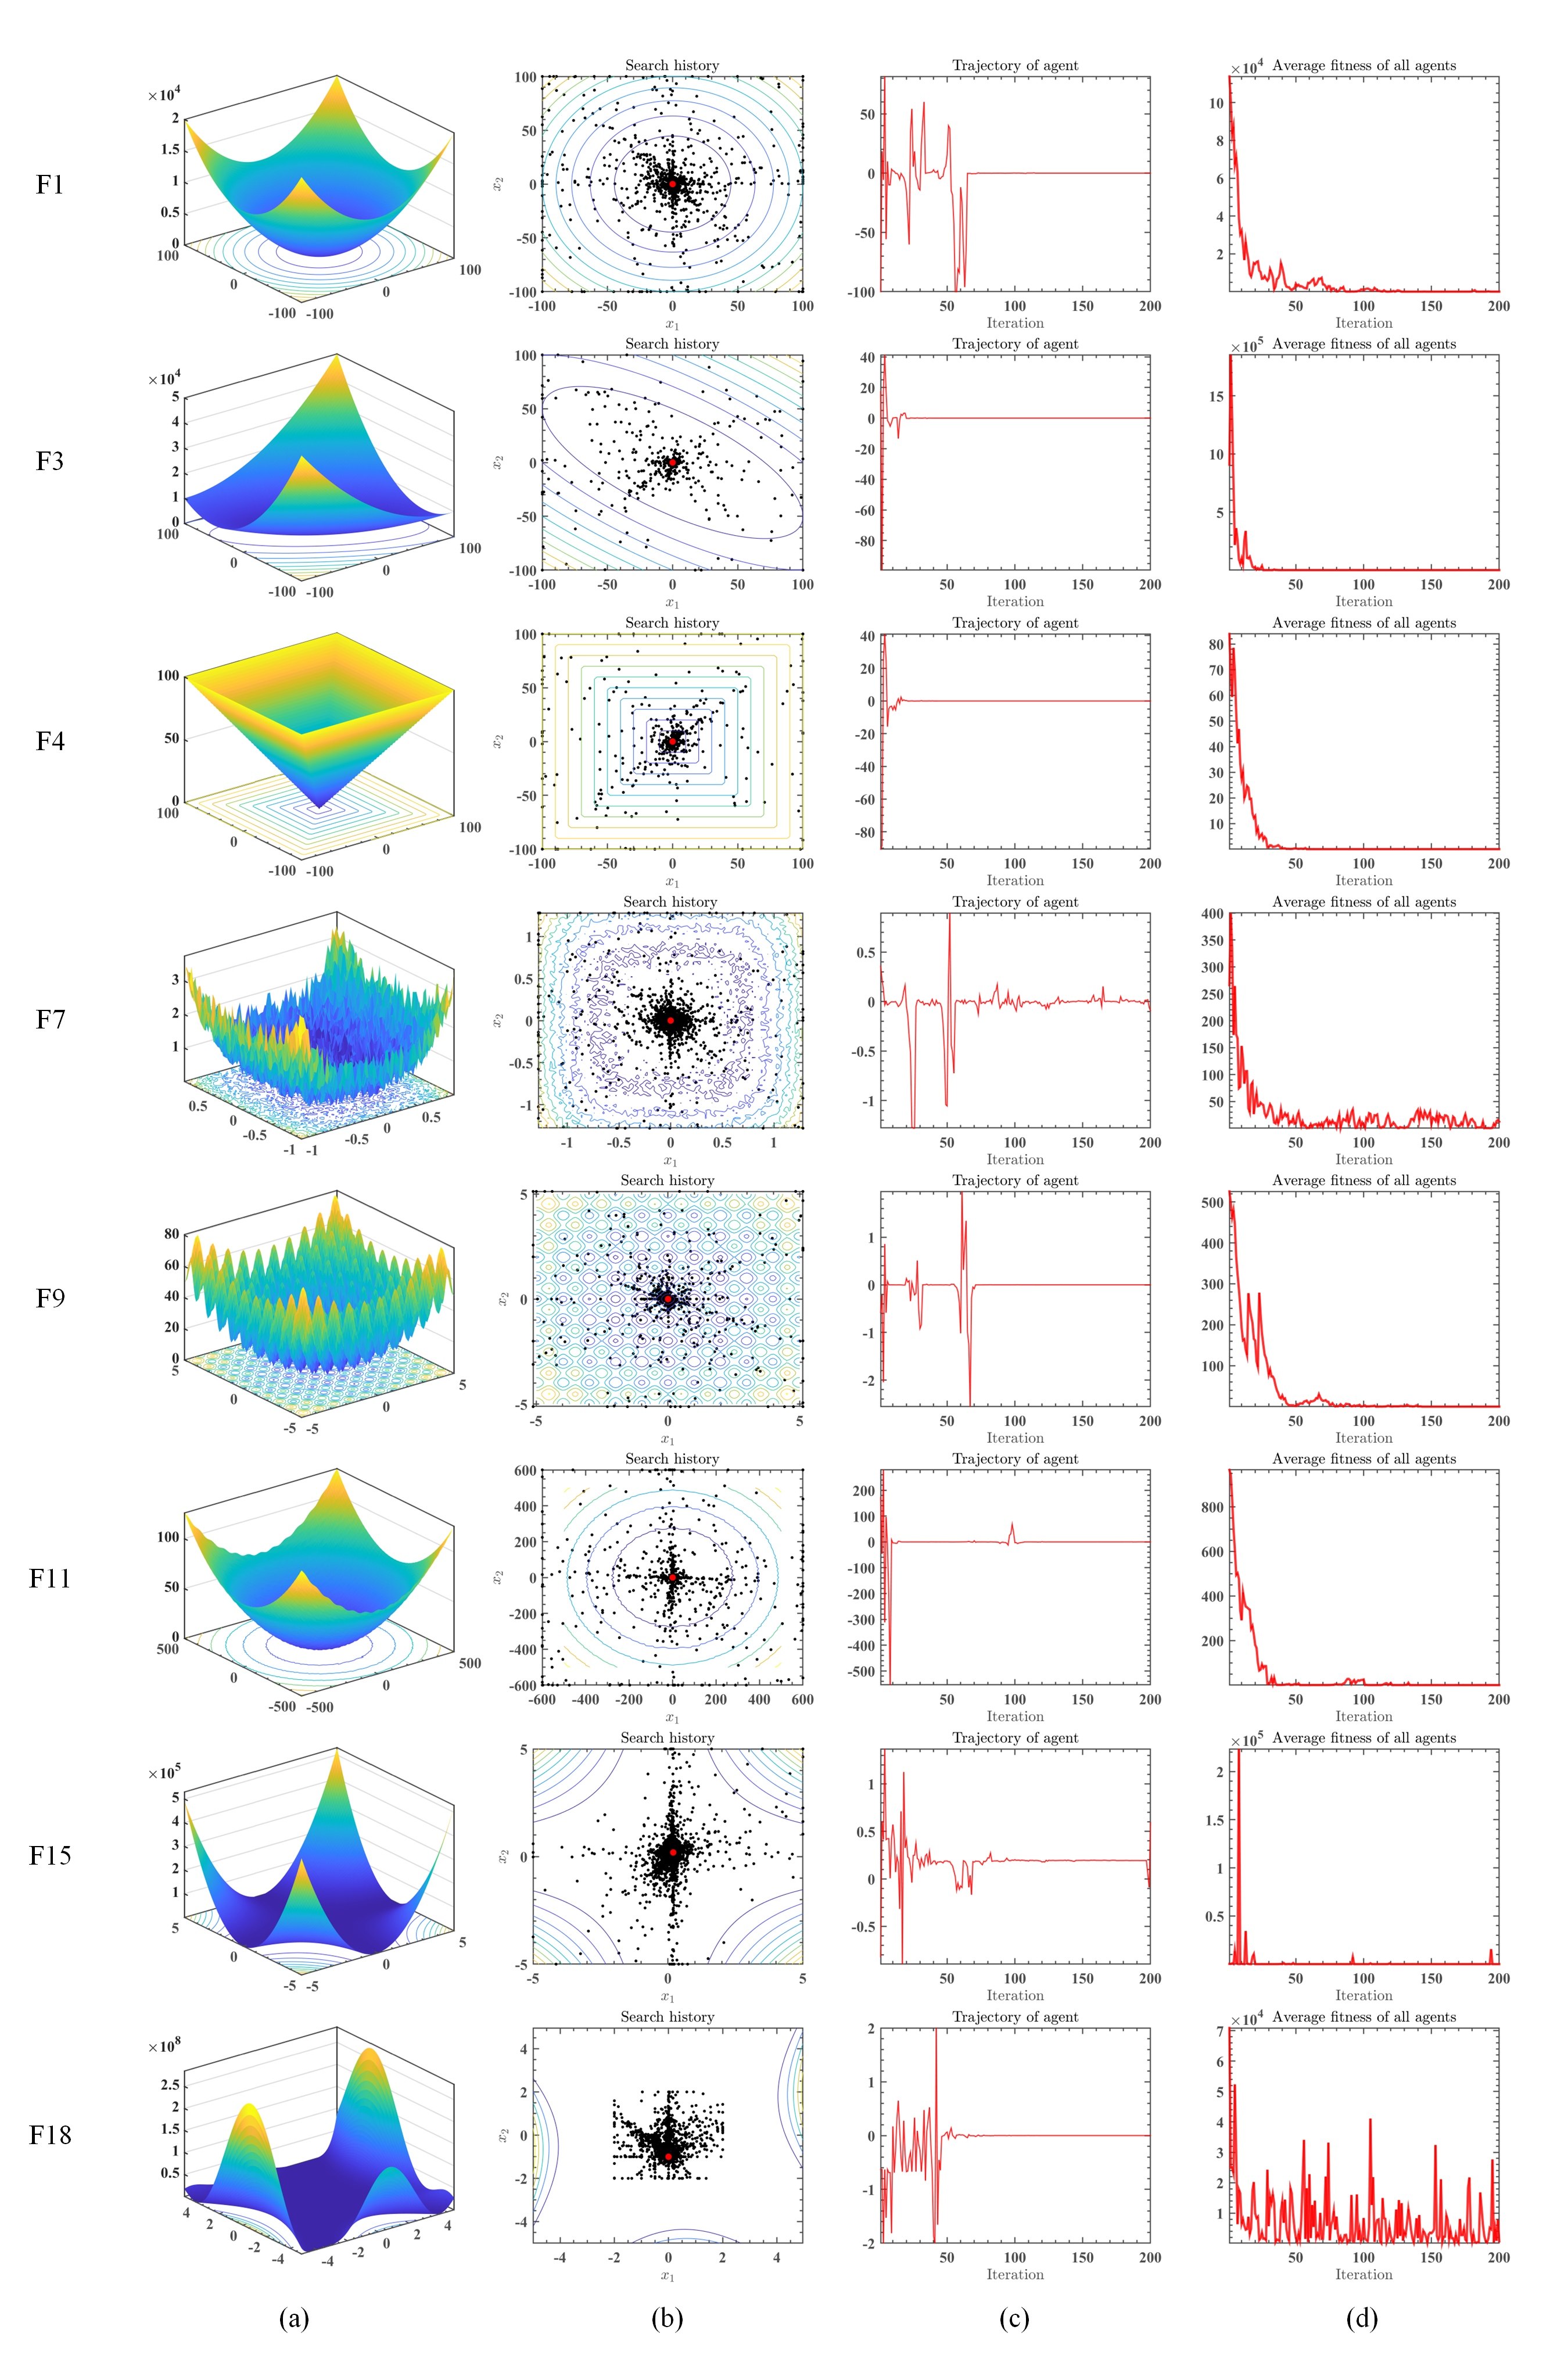
\includegraphics[width=\textwidth]{figures/fig06_search_history_trajectory.png}
  \caption{(a) 3D plots of functions (b) search history, (c) trajectory of agent, (d) average fitness of all agents.}
  \label{fig:search_history_trajectory}
\end{figure}



The comprehensive performance analysis of the SBO algorithm offers significant insights into its functioning, with particular attention to how candidate solutions evolve and improve throughout the optimization process. This analysis demonstrates the efficacy of SBO's unique strategic phases---Elite Engagement and Resource Acquisition---which are based on human status-seeking behaviors. By replicating the human pursuit of upward social mobility, the algorithm drives extensive exploration of the search space, reflecting the natural drive to advance through connections with accomplished individuals. At the same time, the strategic exchange of information and resources among elite agents enables focused exploitation, improving candidate solutions. This effective integration of exploration and exploitation, rooted in status-driven social dynamics, gives SBO strong capabilities for solving complex optimization challenges.


\paragraph{ Benchmark Comparison of SBO}

The~IEEE CEC 2017 benchmark suite's 29 functions~were used~to thoroughly evaluate the proposed SBO algorithm's performance~across~different dimensions and function types.~Testing covered~dimensions of 10, 30, 50, and 100~to examine~scalability.

\textbf{Function categories included}:

\begin{enumerate}
\item  \textbf{Unimodal (F1-F2)}: Tested exploitation and convergence

\item  \textbf{Multimodal (F3-F9)}: Assessed local optima avoidance and exploration

\item  \textbf{Hybrid (F10-F19)}~and~\textbf{composition (F20-F29)}: Evaluated balance between exploration/exploitation
\end{enumerate}

These carefully selected functions~(detailed in Table 1) create~a rigorous test environment~for analyzing SBO's performance characteristics.



\noindent \textbf{}

\begin{tabular}{|p{0.3in}|p{1.5in}|p{0.5in}|p{0.5in}|p{0.5in}|p{0.5in}|} \hline 
\multicolumn{6}{|p{1in}|}{\textbf{Table }1\textbf{.} Information of IEEE CEC 2017.\textbf{}} \\ \hline 
ID & Description & Type & Dimension & Range & Optimum \\ \hline 
F1 & Shifted and Rotated Bent Cigar Function & Unimodal & 10,30,50,100 & [-100,100] & 100 \\ \hline 
F2 & Shifted and Rotated Zakharov function & Unimodal & 10,30,50,100 & [-100,100] & 300 \\ \hline 
F3 & Shifted and Rotated Rosenbrock's function & Multimodal & 10,30,50,100 & [-100,100] & 400 \\ \hline 
F4 & Shifted and Rotated Rastrigin's function & Multimodal & 10,30,50,100 & [-100,100] & 500 \\ \hline 
F5 & Shifted and Rotated Expanded Scaffer's function & Multimodal & 10,30,50,100 & [-100,100] & 600 \\ \hline 
F6 & Shifted and Rotated Lunacek Bi-Rastrigin function & Multimodal & 10,30,50,100 & [-100,100] & 700 \\ \hline 
F7 & Shifted and Rotated Non-Continuous Rastrigin's function & Multimodal & 10,30,50,100 & [-100,100] & 800 \\ \hline 
F8 & Shifted and Rotated L\'{e}vy function & Multimodal & 10,30,50,100 & [-100,100] & 900 \\ \hline 
F9 & Shifted and Rotated Schwefel's function & Multimodal & 10,30,50,100 & [-100,100] & 1000 \\ \hline 
F10 & Hybrid Function 1 (N=3) & Hybrid & 10,30,50,100 & [-100,100] & 1100 \\ \hline 
F11 & Hybrid Function 2 (N=3) & Hybrid & 10,30,50,100 & [-100,100] & 1200 \\ \hline 
F12 & Hybrid Function 3 (N=3) & Hybrid & 10,30,50,100 & [-100,100] & 1300 \\ \hline 
F13 & Hybrid Function 4 (N=4) & Hybrid & 10,30,50,100 & [-100,100] & 1400 \\ \hline 
F14 & Hybrid Function 5 (N=4) & Hybrid & 10,30,50,100 & [-100,100] & 1500 \\ \hline 
F15 & Hybrid Function 6 (N=4) & Hybrid & 10,30,50,100 & [-100,100] & 1600 \\ \hline 
F16 & Hybrid Function 6 (N=5) & Hybrid & 10,30,50,100 & [-100,100] & 1700 \\ \hline 
F17 & Hybrid Function 6 (N=5) & Hybrid & 10,30,50,100 & [-100,100] & 1800 \\ \hline 
F18 & Hybrid Function 6 (N=5) & Hybrid & 10,30,50,100 & [-100,100] & 1900 \\ \hline 
F19 & Hybrid Function 6 (N=6) & Hybrid & 10,30,50,100 & [-100,100] & 2000 \\ \hline 
F20 & Composition Function 1 (N=3) & Composition & 10,30,50,100 & [-100,100] & 2100 \\ \hline 
F21 & Composition Function 2 (N=3) & Composition & 10,30,50,100 & [-100,100] & 2200 \\ \hline 
F22 & Composition Function 3 (N=4) & Composition & 10,30,50,100 & [-100,100] & 2300 \\ \hline 
F23 & Composition Function 4 (N=4) & Composition & 10,30,50,100 & [-100,100] & 2400 \\ \hline 
F24 & Composition Function 5 (N=5) & Composition & 10,30,50,100 & [-100,100] & 2500 \\ \hline 
F25 & Composition Function 6 (N=5) & Composition & 10,30,50,100 & [-100,100] & 2600 \\ \hline 
F26 & Composition Function 7 (N=6) & Composition & 10,30,50,100 & [-100,100] & 2700 \\ \hline 
F27 & Composition Function 8 (N=6) & Composition & 10,30,50,100 & [-100,100] & 2800 \\ \hline 
F28 & Composition Function 9 (N=3) & Composition & 10,30,50,100 & [-100,100] & 2900 \\ \hline 
F29 & Composition Function 10 (N=3) & Composition & 10,30,50,100 & [-100,100] & 3000 \\ \hline 
\end{tabular}



To validate the SBO, a comparative analysis was conducted with 13 state-of-the-art algorithms, chosen based on their diversity, relevance, and performance merits in prior studies. These algorithms represent a variety of optimization strategies, including human-behavior-inspired approaches, swarm intelligence, and evolutionary techniques. This selection includes two human-behavior inspired algorithms, namely the renowned TLBO [30] and the widely acknowledged PO [37], as well as two recently proposed algorithms with significant citations: Harris Hawks Optimization (HHO) [48] and a physical-based optimization algorithm, RIME [49]. Additionally, the comparison featured four acclaimed and potent PSO variants: PSO with Aging Leader and Challengers (ALCPSO) [50], Comprehensive Learning Particle Swarm Optimization (CLPSO) [51], Cooperatively Coevolving Particle Swarm Optimization (CGPSO) [52], and A Multi-Swarm Particle Swarm Optimization (MSPSO) [53]. Complementing these were five evolutionary algorithms known for their championship status: Covariance Matrix Adaptation Evolution Strategy (CMAES) [54], Differential Evolution with a Chaotic Local Search (DECLS) [55], Ensemble Sinusoidal Differential Covariance Matrix Adaptation with Euclidean Neighborhood (LSHADE\_cnEpSin) [56], Sine Cosine Algorithm Differential Evolution (SCADE) [57], and Success-History Based Parameter Adaptation for Differential Evolution (SHADE) [58]. Table 2 summarizes the key characteristics and parameter settings for these algorithms.

To ensure~objective comparison, the parameter settings for each algorithm~followed~the values recommended in their original publications. These settings~maintained consistency~with their intended design and~represented~optimal or near-optimal configurations~as established~in previous studies. All algorithms~operated under identical~computational conditions:

\begin{enumerate}
\item  Fixed population size: 30

\item  Maximum function evaluations: 300,000

\item  Same~termination criteria
\end{enumerate}

This standardized approach~ensured~fair~comparisons~while~avoiding~algorithm-specific tuning~due to computational~limitations.

Analysis results~(Avg and Std over 30 independent runs)~demonstrate~the algorithms' stability and robustness~when solving~the benchmark functions.~While~our methodology~ensures~fairness, we acknowledge that~individual parameter tuning~could further improve performance~and influence~results. Future research~will investigate~this aspect~for more complete~benchmarking.

Furthermore, statistical assessments, such as the Friedman test [59] and the Wilcoxon signed-rank test [60], were employed to analyze the results due to the stochastic nature of the algorithms. These statistical tests, complemented by the average value and standard deviation, ascertained the overall performance and benchmarked the statistical significance of the comparative results. Notably, the significance threshold was set at 0.05, with the resulting p-values indicative of statistical significance between the proposed SBO and its competitors. Tables will subsequently illustrate the comprehensive comparison of p-values across the four distinct dimensions following the benchmark results.

\noindent 

\begin{tabular}{|p{1.1in}|p{2.8in}|} \hline 
\multicolumn{2}{|p{1in}|}{\textbf{Table }2\textbf{.} Parameter settings for involved algorithms.} \\ \hline 
Algorithm & Other parameters \\ \hline 
TLBO & $None$\textit{} \\ \hline 
PO & $λ=1,n=7$\textit{} \\ \hline 
HHO & $E=\left[-2,2\right]$\textit{} \\ \hline 
RIME & $W=5$\textit{} \\ \hline 
ALCPSO & $w=0.4,c1=2,c2=2,lifespan=60,\ T=2,pro=1/D$\textit{} \\ \hline 
CLPSO & $w_{max}=0.9,w_{min}=0.4,c=1.49445$\textit{} \\ \hline 
CGPSO & $v_{max}=6,c1=2,c2=2$MSPSO \\ \hline 
$v_{max}\mathrm{=6,}v_{\mathrm{min}}\mathrm{=-6,}w_{\mathrm{max}}\mathrm{=0.9,}w_{\mathrm{min}}\mathrm{=0.2,c1=2,c2=2}$CMAES & $λ=4+\left\lfloor 3{ln \left(N\right)\ }\right\rfloor ,w'_i={ln \left(\frac{λ+1}{2}\right)-lni,\ }μ=\left\lfloor \frac{λ}{2}\right\rfloor ,\ {σ=0.3,C}_c=\frac{4}{N+4}$DECLS \\ \hline 
$NP=D,F=0.5,p_{CR}\mathrm{=0.5,L=}\frac{\mathrm{D}}{\mathrm{5}}\mathrm{,m=1500}$LSHADE\_cnEpSin & $NP_{max}=18\times D,NP_{min}=4,H=5,\left|A\right|=1.4\times NP,p=0.11\ $\textit{} \\ \hline 
SCADE & $β_{max}=0.8,β_{min}=0.2,p_{CR}=0.8$\textit{} \\ \hline 
SHADE & $\left|A\right|=2\times NP,p=0.1$ \\ \hline 
 \\ \hline 
 \\ \hline 
\end{tabular}




\paragraph{ Benchmark Results and Statistical Analysis}

The SBO algorithm was comprehensively evaluated against 13 state-of-the-art algorithms using the IEEE CEC 2017 benchmark suite, which includes 29 functions spanning unimodal, multimodal, hybrid, and composition types. These functions were tested across four dimensions (10, 30, 50, and 100) to assess SBO's scalability, robustness, and adaptability to varying problem complexities. The comparative results, including Avg and Std across 30 independent runs, are provided in Table A. 1\textbf{--A.4}, with corresponding p-values detailed in Table A. 5\textbf{--A.8}. Statistical tests, including the Friedman test and Wilcoxon signed-rank test, were performed to evaluate the significance of the results, and their summarized statistics are presented in Table 3.

SBO demonstrated strong and consistent performance across all dimensions, achieving average first-place rankings in 36\% of the benchmark functions. Its strengths were particularly evident in hybrid and composition functions, where balancing exploration and exploitation is critical. A heatmap (Fig. 7) visualizes the normalized performance of all algorithms across functions and dimensions, with warmer colors indicating superior results. In this visualization, SBO frequently stands out as one of the top-performing algorithms, particularly for higher-dimensional hybrid and composition functions, showcasing its adaptability to complex optimization problems.



\begin{figure}[htbp]
  \centering
  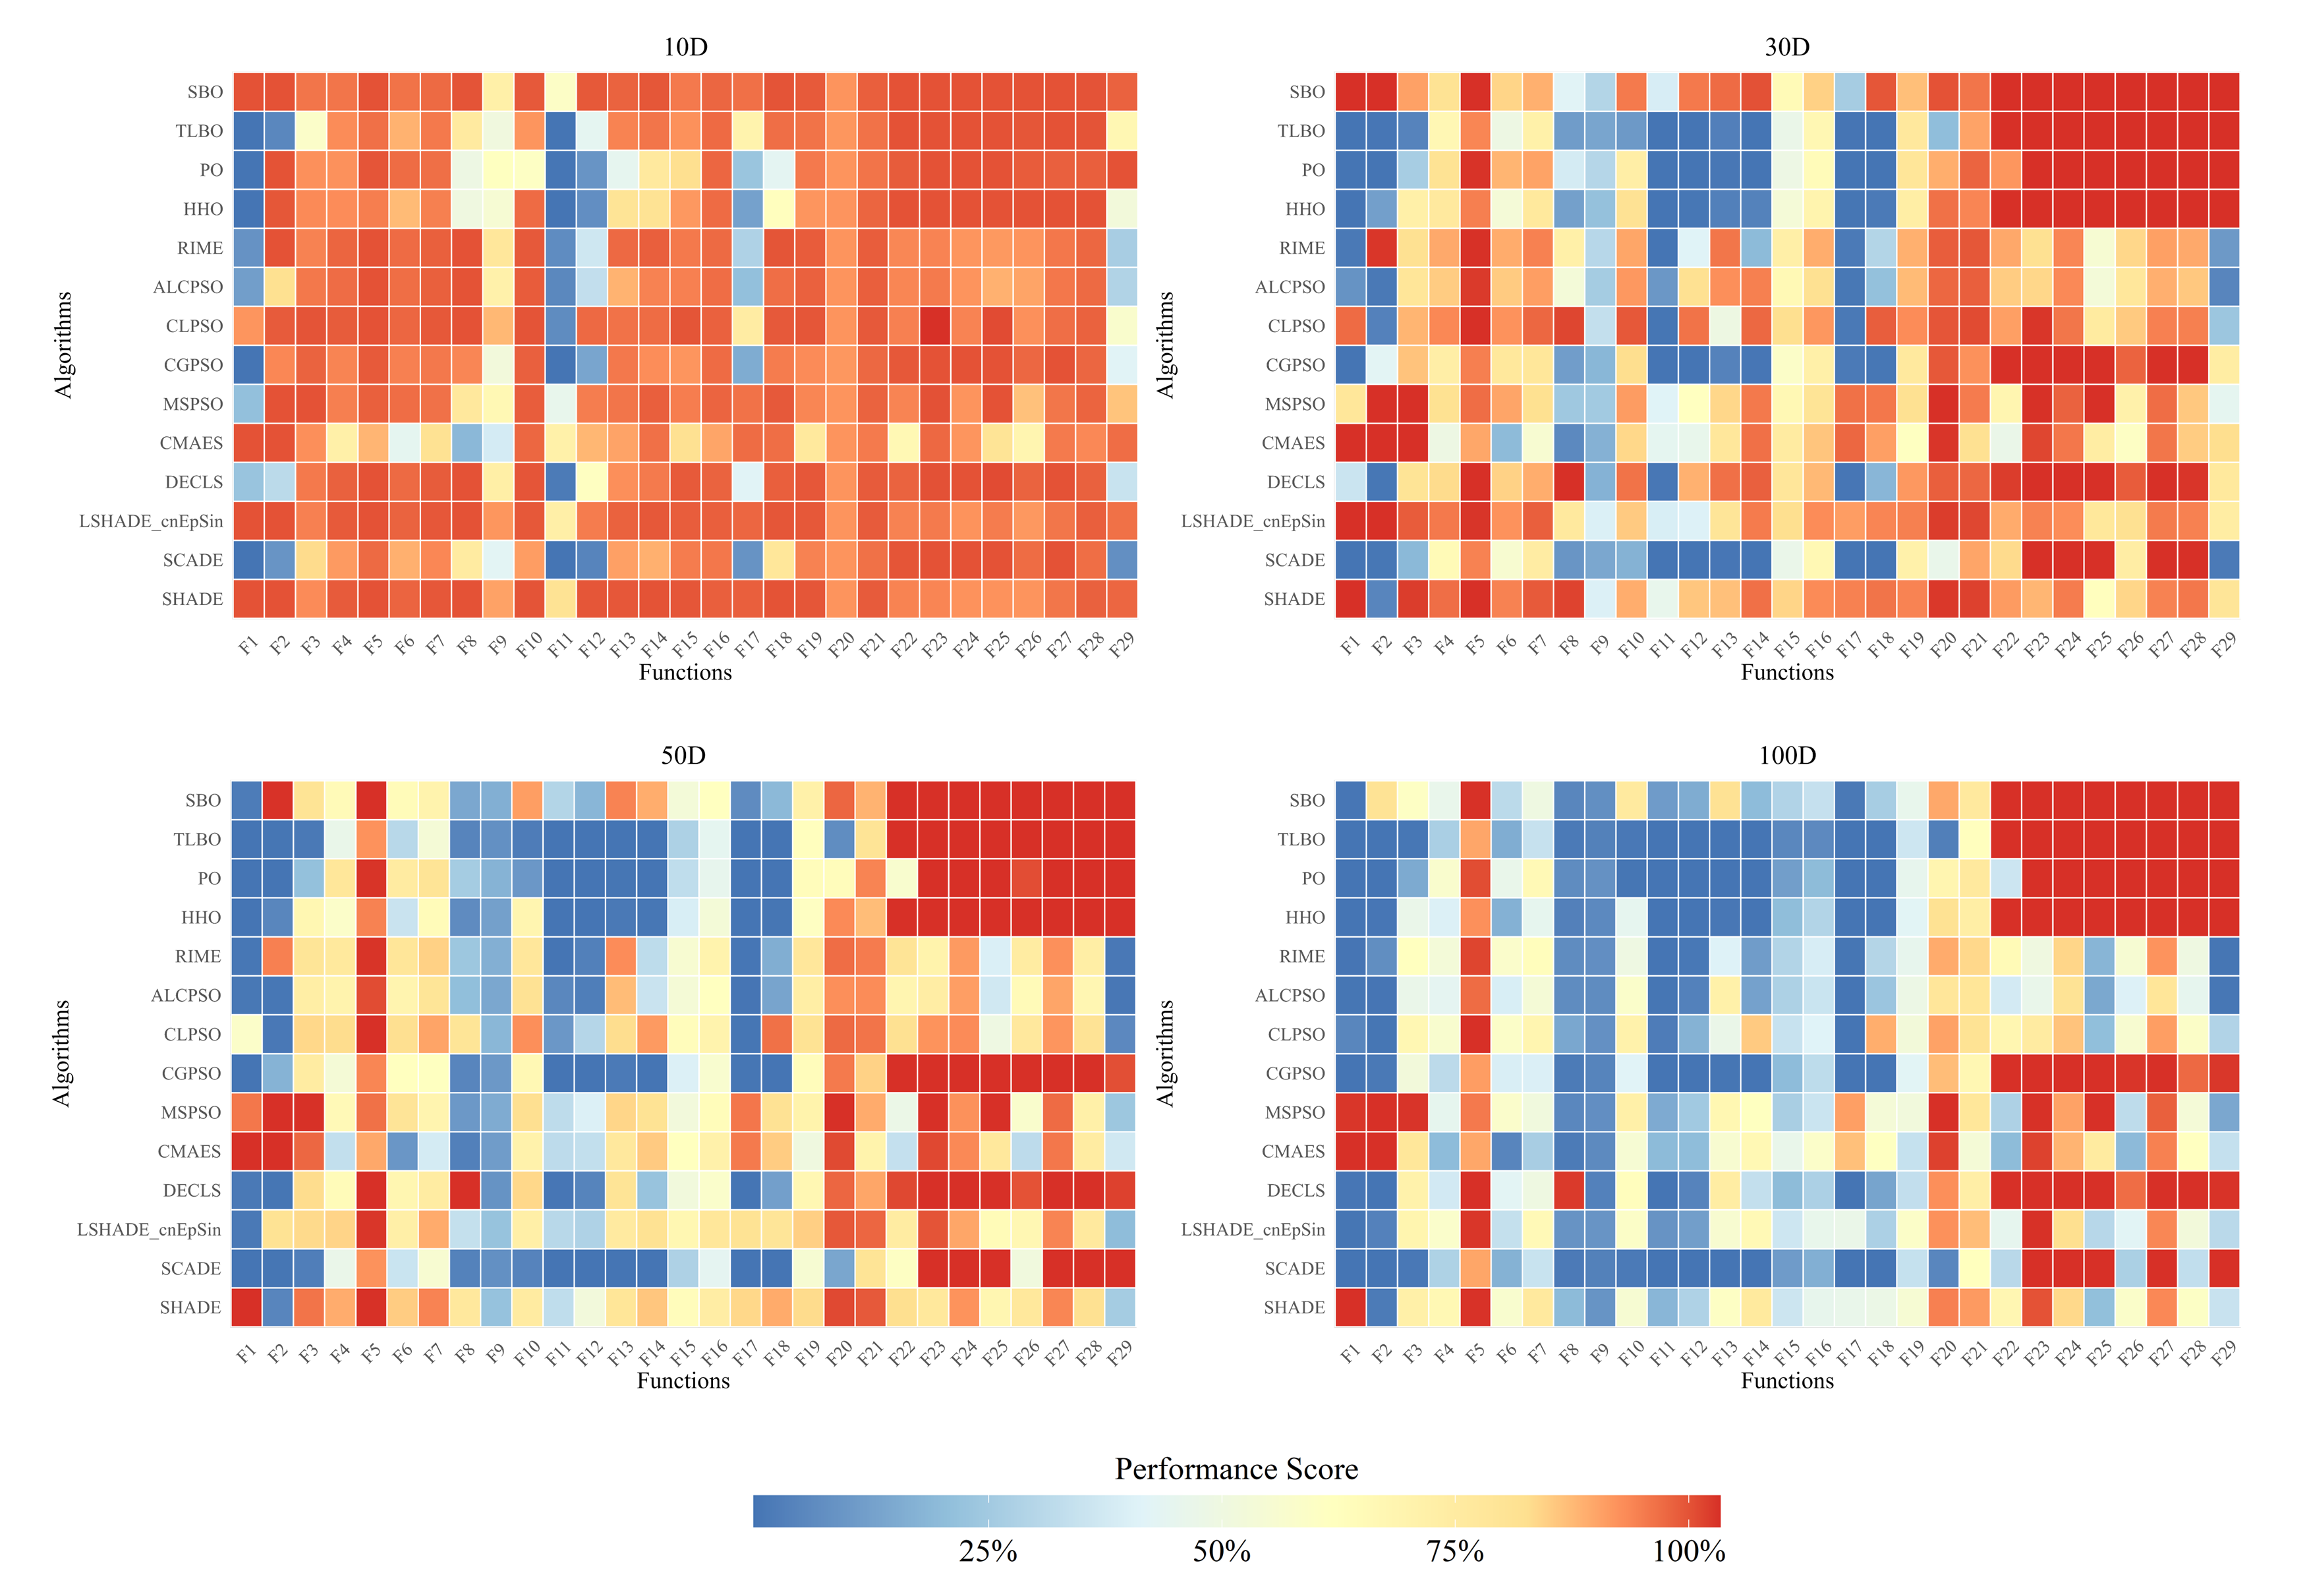
\includegraphics[width=\textwidth]{figures/fig07_performance_heatmap.png}
  \caption{Algorithm performance heatmap across four dimensions.}
  \label{fig:performance_heatmap}
\end{figure}



In unimodal functions (F1--F2), which focus on exploitation and precision, SBO ranked competitively but was slightly outperformed by precision-focused algorithms such as CMAES, LSHADE\_cnEpSin, and LSHADE. On average, SBO secured fourth place in this category across all dimensions, demonstrating its robustness despite a minor trade-off in precision. For multimodal functions (F3--F9), SBO exhibited strong exploratory capabilities, consistently avoiding local optima and achieving competitive rankings. For example, it secured fourth place in F5 while maintaining high stability across the category. The algorithm's performance was most pronounced in hybrid (F10--F19) and composition functions (F20--F29), where it consistently achieved first-place rankings in functions such as F13, F14, and F22--F29. These results highlight SBO's ability to adapt effectively to dynamic landscapes that require a balance between exploration and exploitation.

The 30-dimensional results provide deeper insights into SBO's performance, particularly its convergence behavior and robustness. Convergence curves (Fig. 8) for selected benchmark functions illustrate SBO's steady improvement in solution quality over iterations. For unimodal functions like F1 and F2, SBO maintained consistent convergence rates, closely trailing CMAES and LSHADE in precision. In hybrid and composition functions, such as F13, F14, and F29, SBO demonstrated superior convergence speed, reflecting its ability to identify promising regions of the search space while avoiding premature stagnation. Additionally, box plots (Fig. 9) of SBO's performance across 30 independent runs reveal its low variance compared to algorithms like TLBO and PO, which exhibited higher variability. This stability underscores SBO's reliability, particularly for hybrid and composition functions, where consistent performance is crucial.



\begin{figure}[htbp]
  \centering
  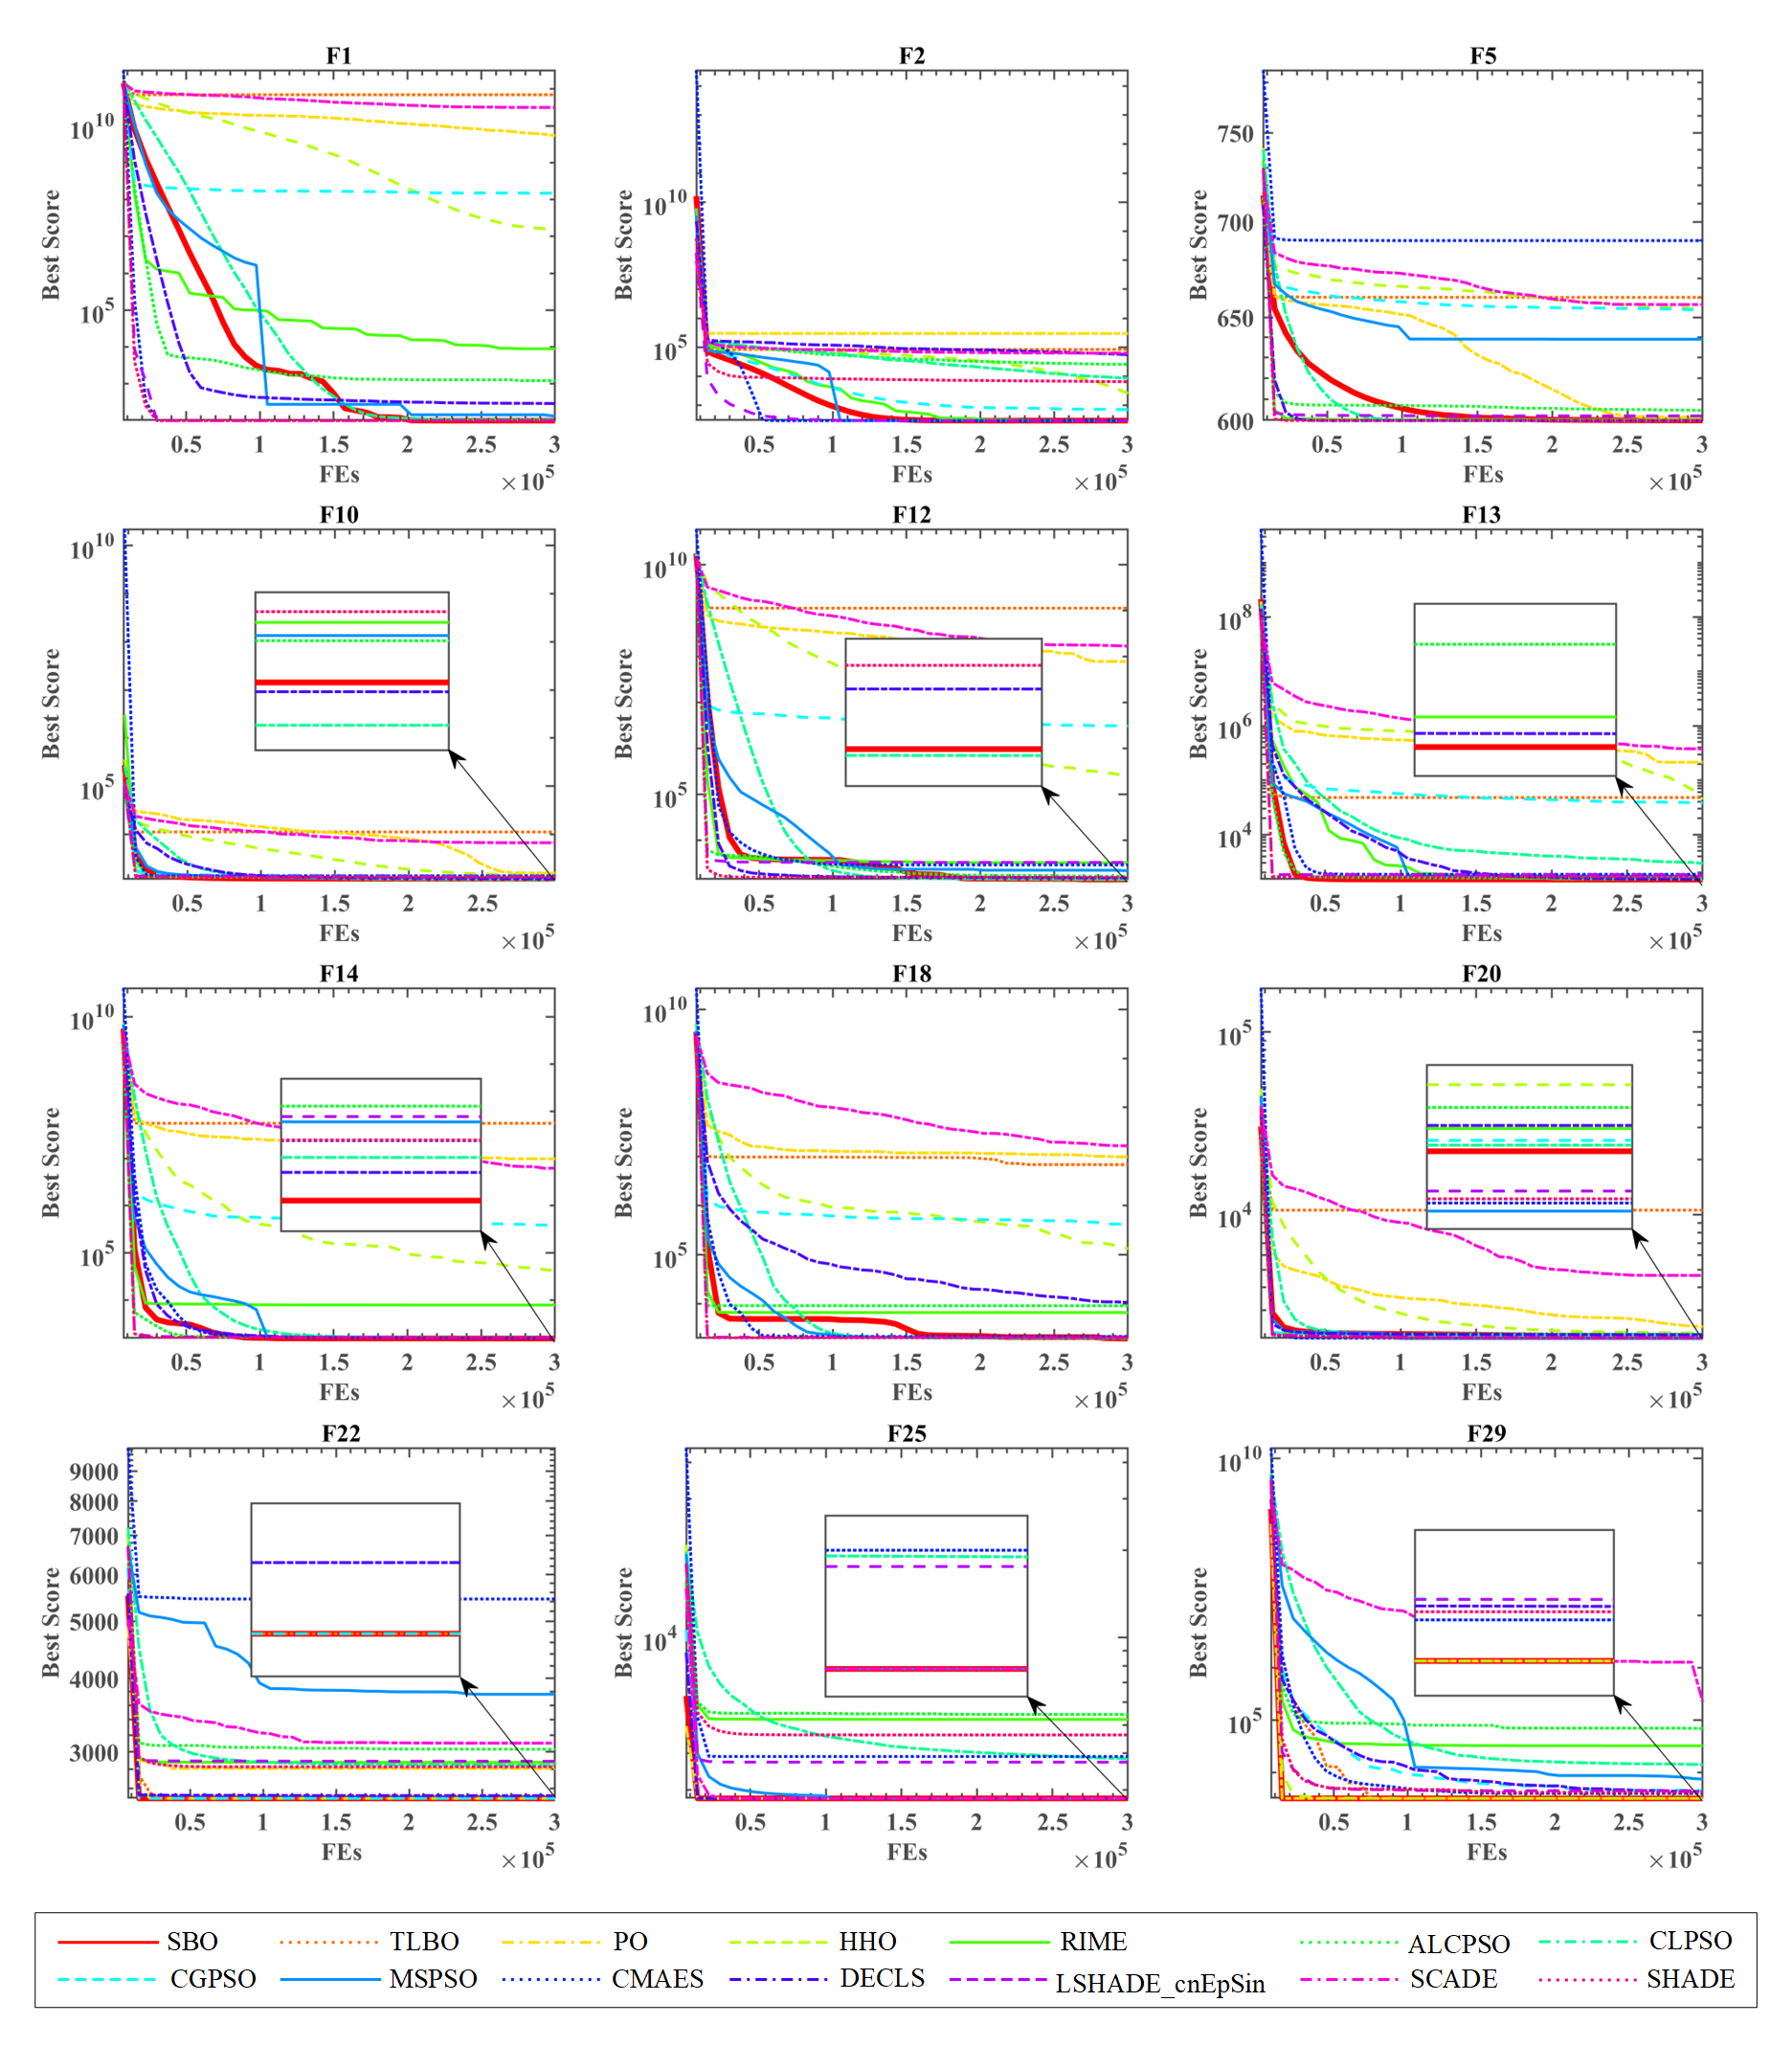
\includegraphics[width=\textwidth]{figures/fig08_convergence_curves_30dim.png}
  \caption{Convergence curves of SBO and state-of-the-art algorithms for 30-dimensional problems.}
  \label{fig:convergence_curves_30dim}
\end{figure}



\begin{figure}[htbp]
  \centering
  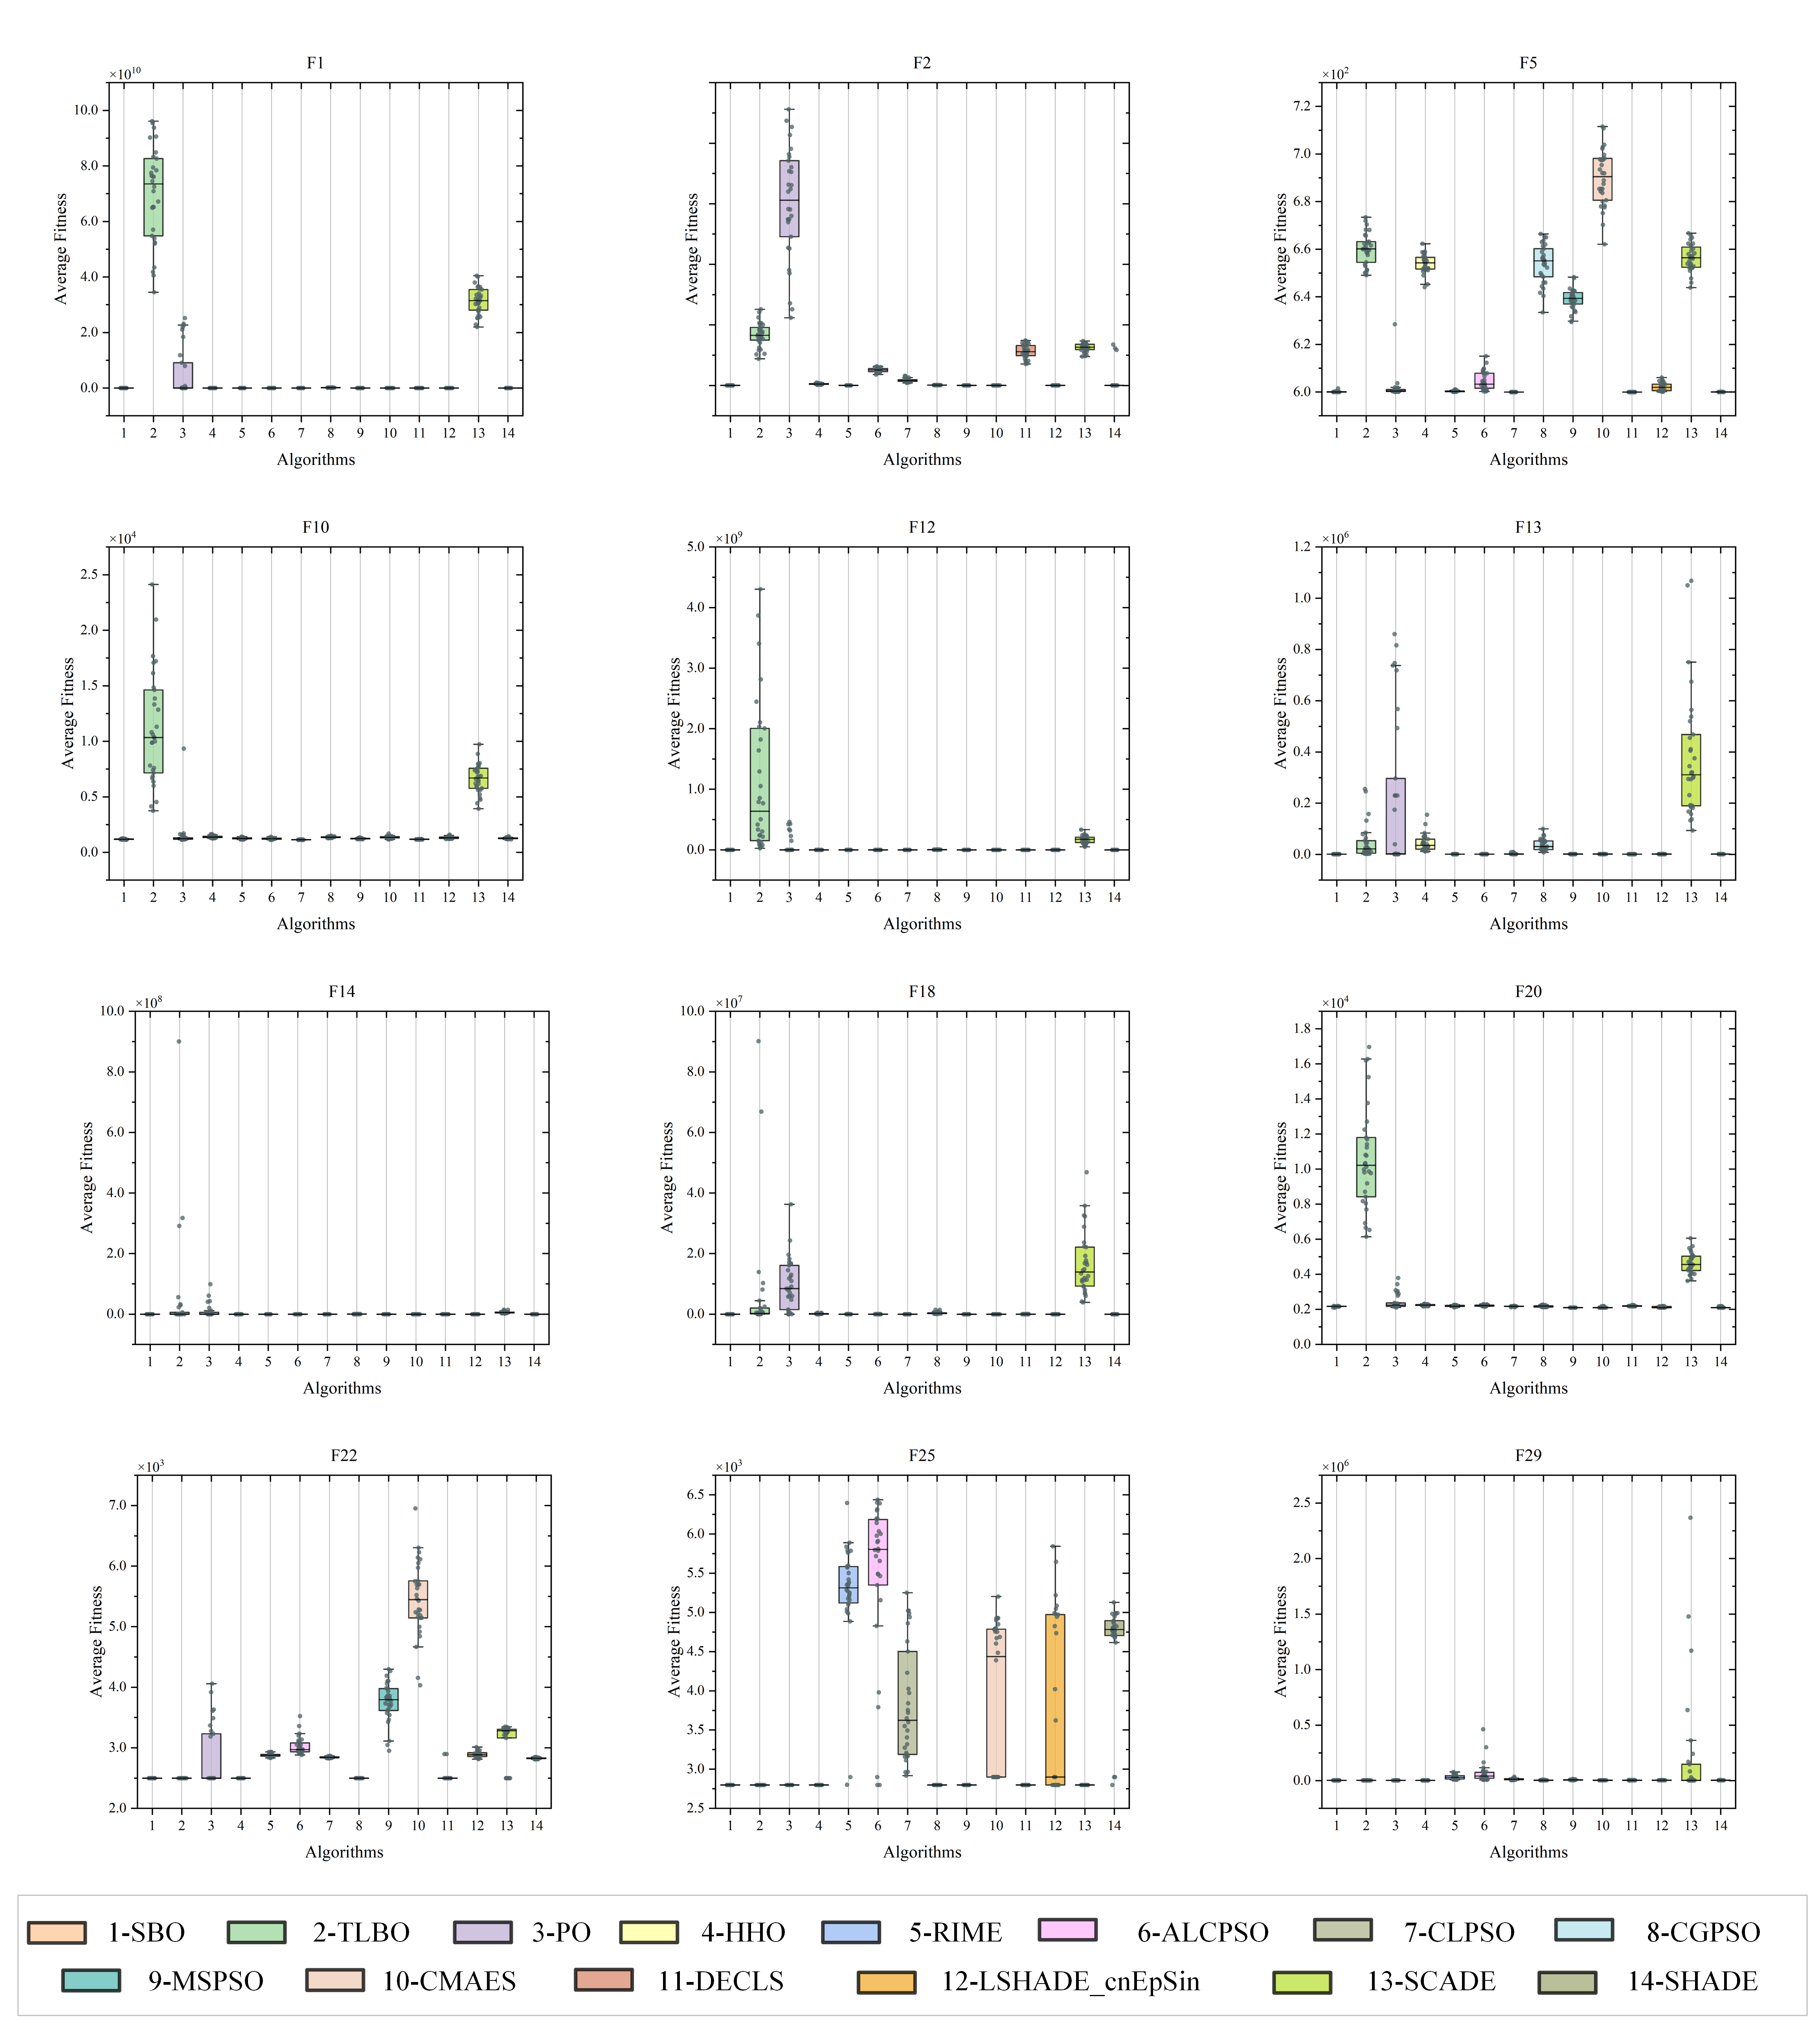
\includegraphics[width=\textwidth]{figures/fig09_box_plots_30dim.png}
  \caption{Box plots comparing SBO and state-of-the-art algorithms for 30-dimensional problems.}
  \label{fig:box_plots_30dim}
\end{figure}



The competitive advantage of SBO is further validated by the statistical analyses. As visualized in Fig. 10, the Friedman test results indicate that SBO achieved the lowest average rank across all dimensions, with values of 3.90, 4.07, 4.38, and 4.48 for 10, 30, 50, and 100 dimensions, respectively. These rankings highlight SBO's scalability and its consistent ability to perform well across varying problem complexities. The Wilcoxon signed-rank test results, summarized in Table 3, reveal that SBO outperformed TLBO, PO, HHO, and RIME in over 70\% of the benchmark functions, with p-values below the significance threshold \eqref{GrindEQ__0_05_}. While its advantage against LSHADE\_cnEpSin and LSHADE was less pronounced, SBO maintained competitiveness, outperforming them in a subset of functions.



\begin{figure}[htbp]
  \centering
  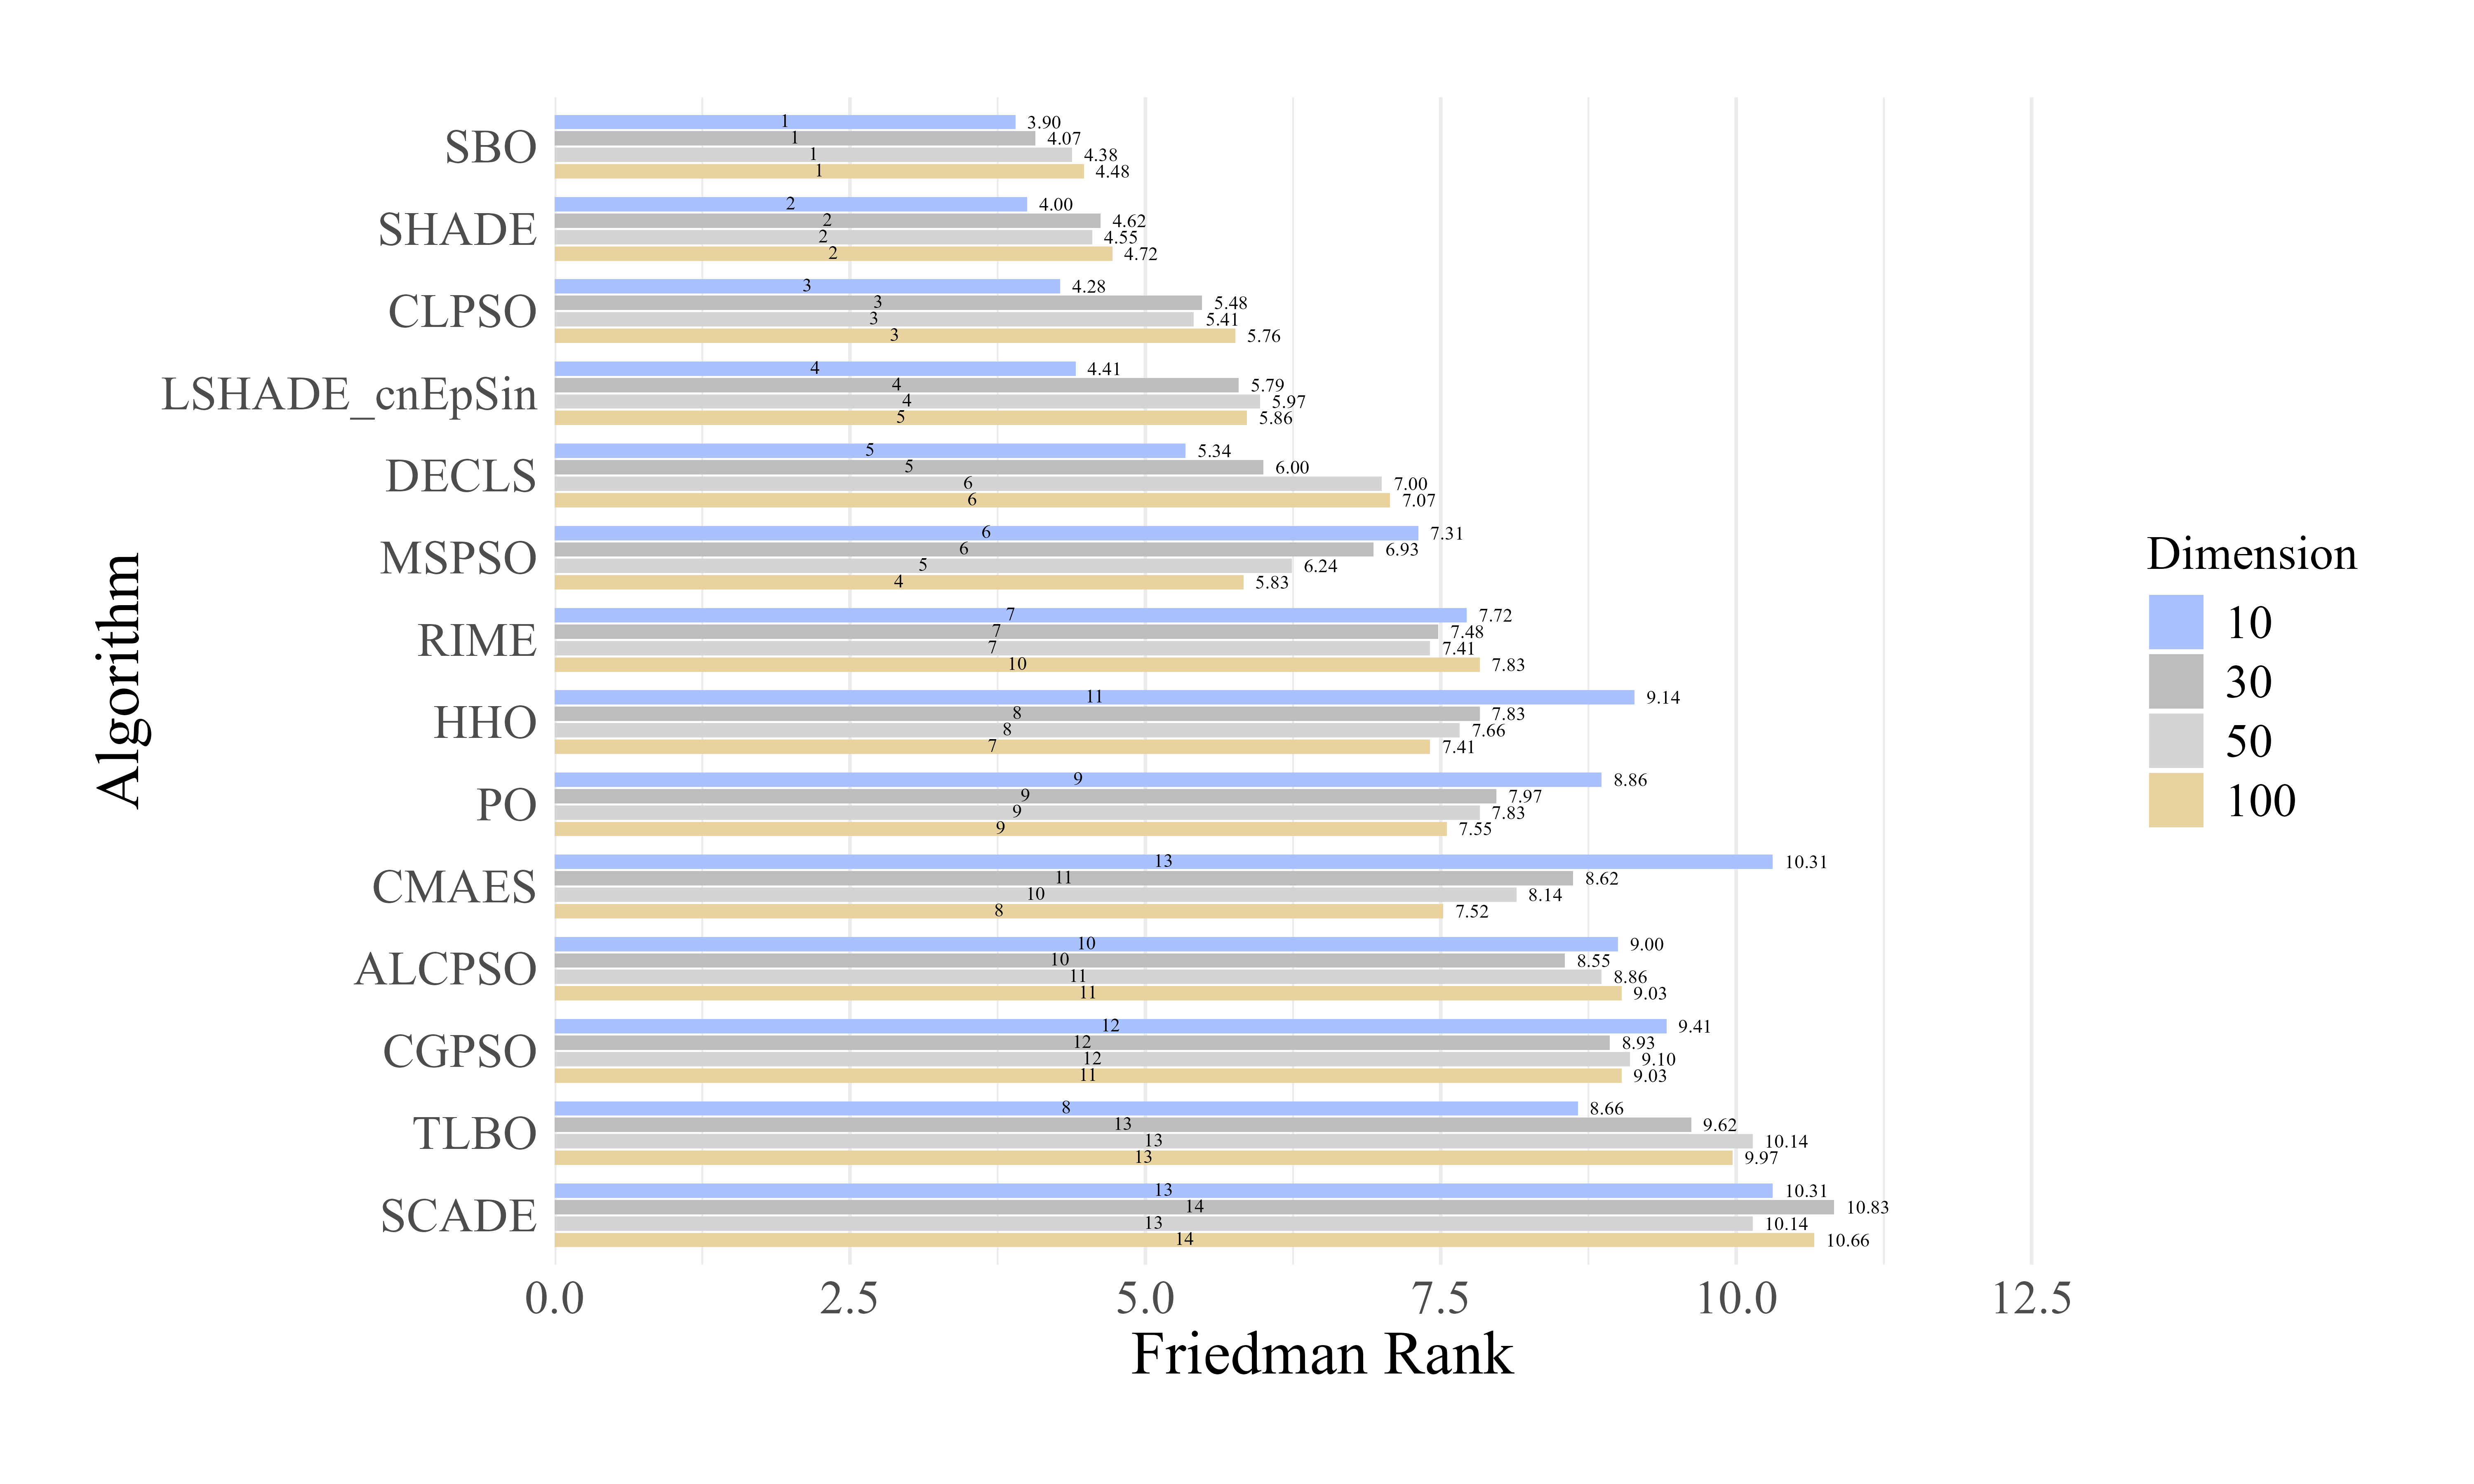
\includegraphics[width=\textwidth]{figures/fig10_friedman_rank.png}
  \caption{Friedman rank result of algorithms across four dimensions.}
  \label{fig:friedman_rank}
\end{figure}



The SBO algorithm's outstanding performance stems from its faithful modeling of status-seeking social behaviors, particularly learning from high-performing peers and strategically retaining beneficial information. These mechanisms enable SBO to achieve an effective balance between exploration and exploitation, allowing it to perform well across both low- and high-dimensional problems. The resource retention strategy of SBO specifically provides it with an advantage in hybrid and composition functions, enabling both rapid convergence and remarkable stability across different runs. Although SBO's performance on unimodal functions was marginally below that of precision-focused algorithms, its overall adaptability, stability, and scalability establish it as a highly capable solution for diverse optimization tasks.

\noindent 

\begin{tabular}{|p{0.5in}|p{0.3in}|p{0.4in}|p{0.4in}|p{0.4in}|p{0.4in}|p{0.8in}|p{0.4in}|p{0.4in}|} \hline 
\multicolumn{9}{|p{1in}|}{\textbf{Table }3\textbf{. }WSRT and FT results of SBO and other algorithms on IEEE CEC 2017.} \\ \hline 
Dimension & Item & SBO & TLBO & PO & HHO & RIME & ALCPSO & CLPSO \\ \hline 
10 & \textbf{+/-/=} & $\mathrm{\sim}$ & 22/0/7 & 18/2/9 & 21/1/7 & 18/6/5 & 18/3/8 & 14/13/2 \\ \hline 
 & Rank\textbf{} & \textbf{3.8966} & 8.6552 & 8.8621 & 9.1379 & 7.7241 & 9.0000 & 4.2759 \\ \hline 
 & Result\textbf{} & \textbf{1} & 8 & 9 & 11 & 7 & 10 & 3 \\ \hline 
30 & \textbf{+/-/=} & $\mathrm{\sim}$\textbf{} & 21/0/8 & 16/2/11 & 21/0/8 & 20/7/2 & 21/4/4 & 15/11/3 \\ \hline 
 & Rank\textbf{} & \textbf{4.0690} & 9.6207 & 7.9655 & 7.8276 & 7.4828 & 8.5517 & 5.4828 \\ \hline 
 & Result\textbf{} & \textbf{1} & 13 & 9 & 8 & 7 & 10 & 3 \\ \hline 
50 & \textbf{+/-/=} & $\mathrm{\sim}$\textbf{} & 21/0/8 & 16/5/8 & 21/0/8 & 17/7/5 & 20/5/4 & 12/13/4 \\ \hline 
 & Rank\textbf{} & \textbf{4.3793} & 10.1379 & 7.8276 & 7.6552 & 7.4138 & 8.8621 & 5.4138 \\ \hline 
 & Result\textbf{} & \textbf{1} & 13 & 9 & 8 & 7 & 11 & 3 \\ \hline 
100 & \textbf{+/-/=} & $\mathrm{\sim}$ & 21/0/8 & 14/5/10 & 21/0/8 & 16/6/7 & 18/5/6 & 13/14/2 \\ \hline 
 & Rank\textbf{} & \textbf{4.4828} & 9.9655 & 7.5517 & 7.4138 & 7.8276 & 9.0345 & 5.7586 \\ \hline 
 & Result\textbf{} & \textbf{1} & 13 & 9 & 7 & 10 & 11 & 3 \\ \hline 
Dimension & Item & CGPSO & MSPSO & CMAES & DECLS & LSHADE\_cnEpSin & SCADE & SHADE \\ \hline 
10 & \textbf{+/-/=} & 28/1/0 & 23/3/3 & 24/1/4 & 14/10/5 & 10/9/10 & 23/0/6 & 8/16/5 \\ \hline 
 & Rank & 9.4138 & 7.3103 & 10.3103 & 5.3448 & 4.4138 & 10.3103 & 4.0000 \\ \hline 
 & Result & 12 & 6 & 13 & 5 & 4 & 13 & 2 \\ \hline 
30 & \textbf{+/-/=} & 27/0/2 & 20/5/4 & 21/6/2 & 18/7/4 & 14/14/1 & 24/0/5 & 14/14/1 \\ \hline 
 & Rank & 8.9310 & 6.9310 & 8.6207 & 6.0000 & 5.7931 & 10.8276 & 4.6207 \\ \hline 
 & Result & 12 & 6 & 11 & 5 & 4 & 14 & 2 \\ \hline 
50 & \textbf{+/-/=} & 29/0/0 & 14/10/5 & 19/9/1 & 20/5/4 & 12/12/5 & 23/0/6 & 13/16/0 \\ \hline 
 & Rank & 9.1034 & 6.2414 & 8.1379 & 7.0000 & 5.9655 & 10.1379 & 4.5517 \\ \hline 
 & Result & 12 & 5 & 10 & 6 & 4 & 13 & 2 \\ \hline 
100 & \textbf{+/-/=} & 28/1/0 & 13/15/1 & 18/10/1 & 21/6/2 & 13/13/3 & 24/0/5 & 11/17/1 \\ \hline 
 & Rank & 9.0345 & 5.8276 & 7.5172 & 7.0690 & 5.8621 & 10.6552 & 4.7241 \\ \hline 
 & Result & 11 & 4 & 8 & 6 & 5 & 14 & 2 \\ \hline 
\end{tabular}




\paragraph{ Runtime Performance Analysis}

To comprehensively evaluate the runtime performance of the proposed SBO algorithm, we conducted experiments using the IEEE CEC 2017 benchmark suite, consisting of 29 distinct functions. Each algorithm, including SBO and 13 state-of-the-art competitors, was executed 30 times independently for each benchmark function across four dimensions: 10, 30, 50, and 100. The runtime performance was measured as the average runtime (in seconds) across all 30 runs for the 29 functions at each dimension. The results are summarized in Table 4 and visualized in Fig. 11.

The algorithms considered in the comparison include TLBO, PO, HHO, a physics-based algorithm RIME, four PSO variants (ALCPSO, CLPSO, CGPSO, and MSPSO), and five evolutionary algorithms (CMAES, DECLS, LSHADE\_cnEpSin, SCADE, and SHADE).

The runtime results reveal that SBO demonstrates competitive performance across all tested dimensions. At the smallest dimension ($D=10$), SBO achieves the second-fastest runtime (28.08 seconds), trailing only CGPSO (27.57 seconds). As the problem dimension increases, SBO consistently ranks as the fastest algorithm, achieving the shortest runtime for dimensions $D=30$, $D=50$, and $D=100$, with average runtimes of 74.25, 151.24, and 478.73 seconds, respectively.

Compared to slower algorithms, such as LSHADE\_cnEpSin and SCADE, SBO exhibits significantly better scalability. The results suggest that SBO's computational efficiency becomes increasingly pronounced in higher dimensions. This improvement can be attributed to the efficient mechanisms employed by SBO, which reduce unnecessary computational overhead during resource evaluation and updates.

The visualization in Fig. 11 highlights SBO's runtime performance across dimensions, showcasing its consistency and scalability. While some algorithms, such as TLBO and ALCPSO, remain competitive, SBO's superior runtime at higher dimensions reinforces its suitability for large-scale optimization tasks.

Despite these findings, it is important to note that runtime performance may vary across computational environments due to differences in hardware and software configurations. Future studies will aim to standardize additional runtime evaluations across diverse platforms to validate these results further.

\noindent 

\noindent \textbf{Table }4\textbf{. }Runtime performance of SBO and other algorithms on IEEE CEC 2017.

\begin{tabular}{|p{0.5in}|p{0.4in}|p{0.4in}|p{0.4in}|p{0.4in}|p{0.8in}|p{0.4in}|p{0.4in}|} \hline 
Dimension & SBO & TLBO & PO & HHO & RIME & ALCPSO & CLPSO \\ \hline 
10 & 28.08  & 32.07  & 60.36  & 59.10  & 48.11  & 39.17  & 39.92  \\ \hline 
30 & \textbf{74.25 } & 77.67  & 101.20  & 107.86  & 88.65  & 92.48  & 107.64  \\ \hline 
50 & \textbf{151.24 } & 155.10  & 190.04  & 217.82  & 175.12  & 157.99  & 181.29  \\ \hline 
100 & \textbf{478.73 } & 483.49  & 551.37  & 683.48  & 531.06  & 496.47  & 535.68  \\ \hline 
Dimension & CGPSO & MSPSO & CMAES & DECLS & LSHADE\_cnEpSin & SCADE & SHADE \\ \hline 
10 & \textbf{27.57 } & 81.57  & 67.94  & 32.75  & 94.44  & 57.67  & 42.16  \\ \hline 
30 & 112.18  & 128.53  & 111.10  & 101.04  & 179.70  & 135.75  & 92.36  \\ \hline 
50 & 180.14  & 160.21  & 177.28  & 182.29  & 248.05  & 259.45  & 176.46  \\ \hline 
100 & 577.42  & 486.66  & 522.08  & 515.72  & 636.77  & 770.86  & 520.70  \\ \hline 
\end{tabular}



\begin{figure}[htbp]
  \centering
  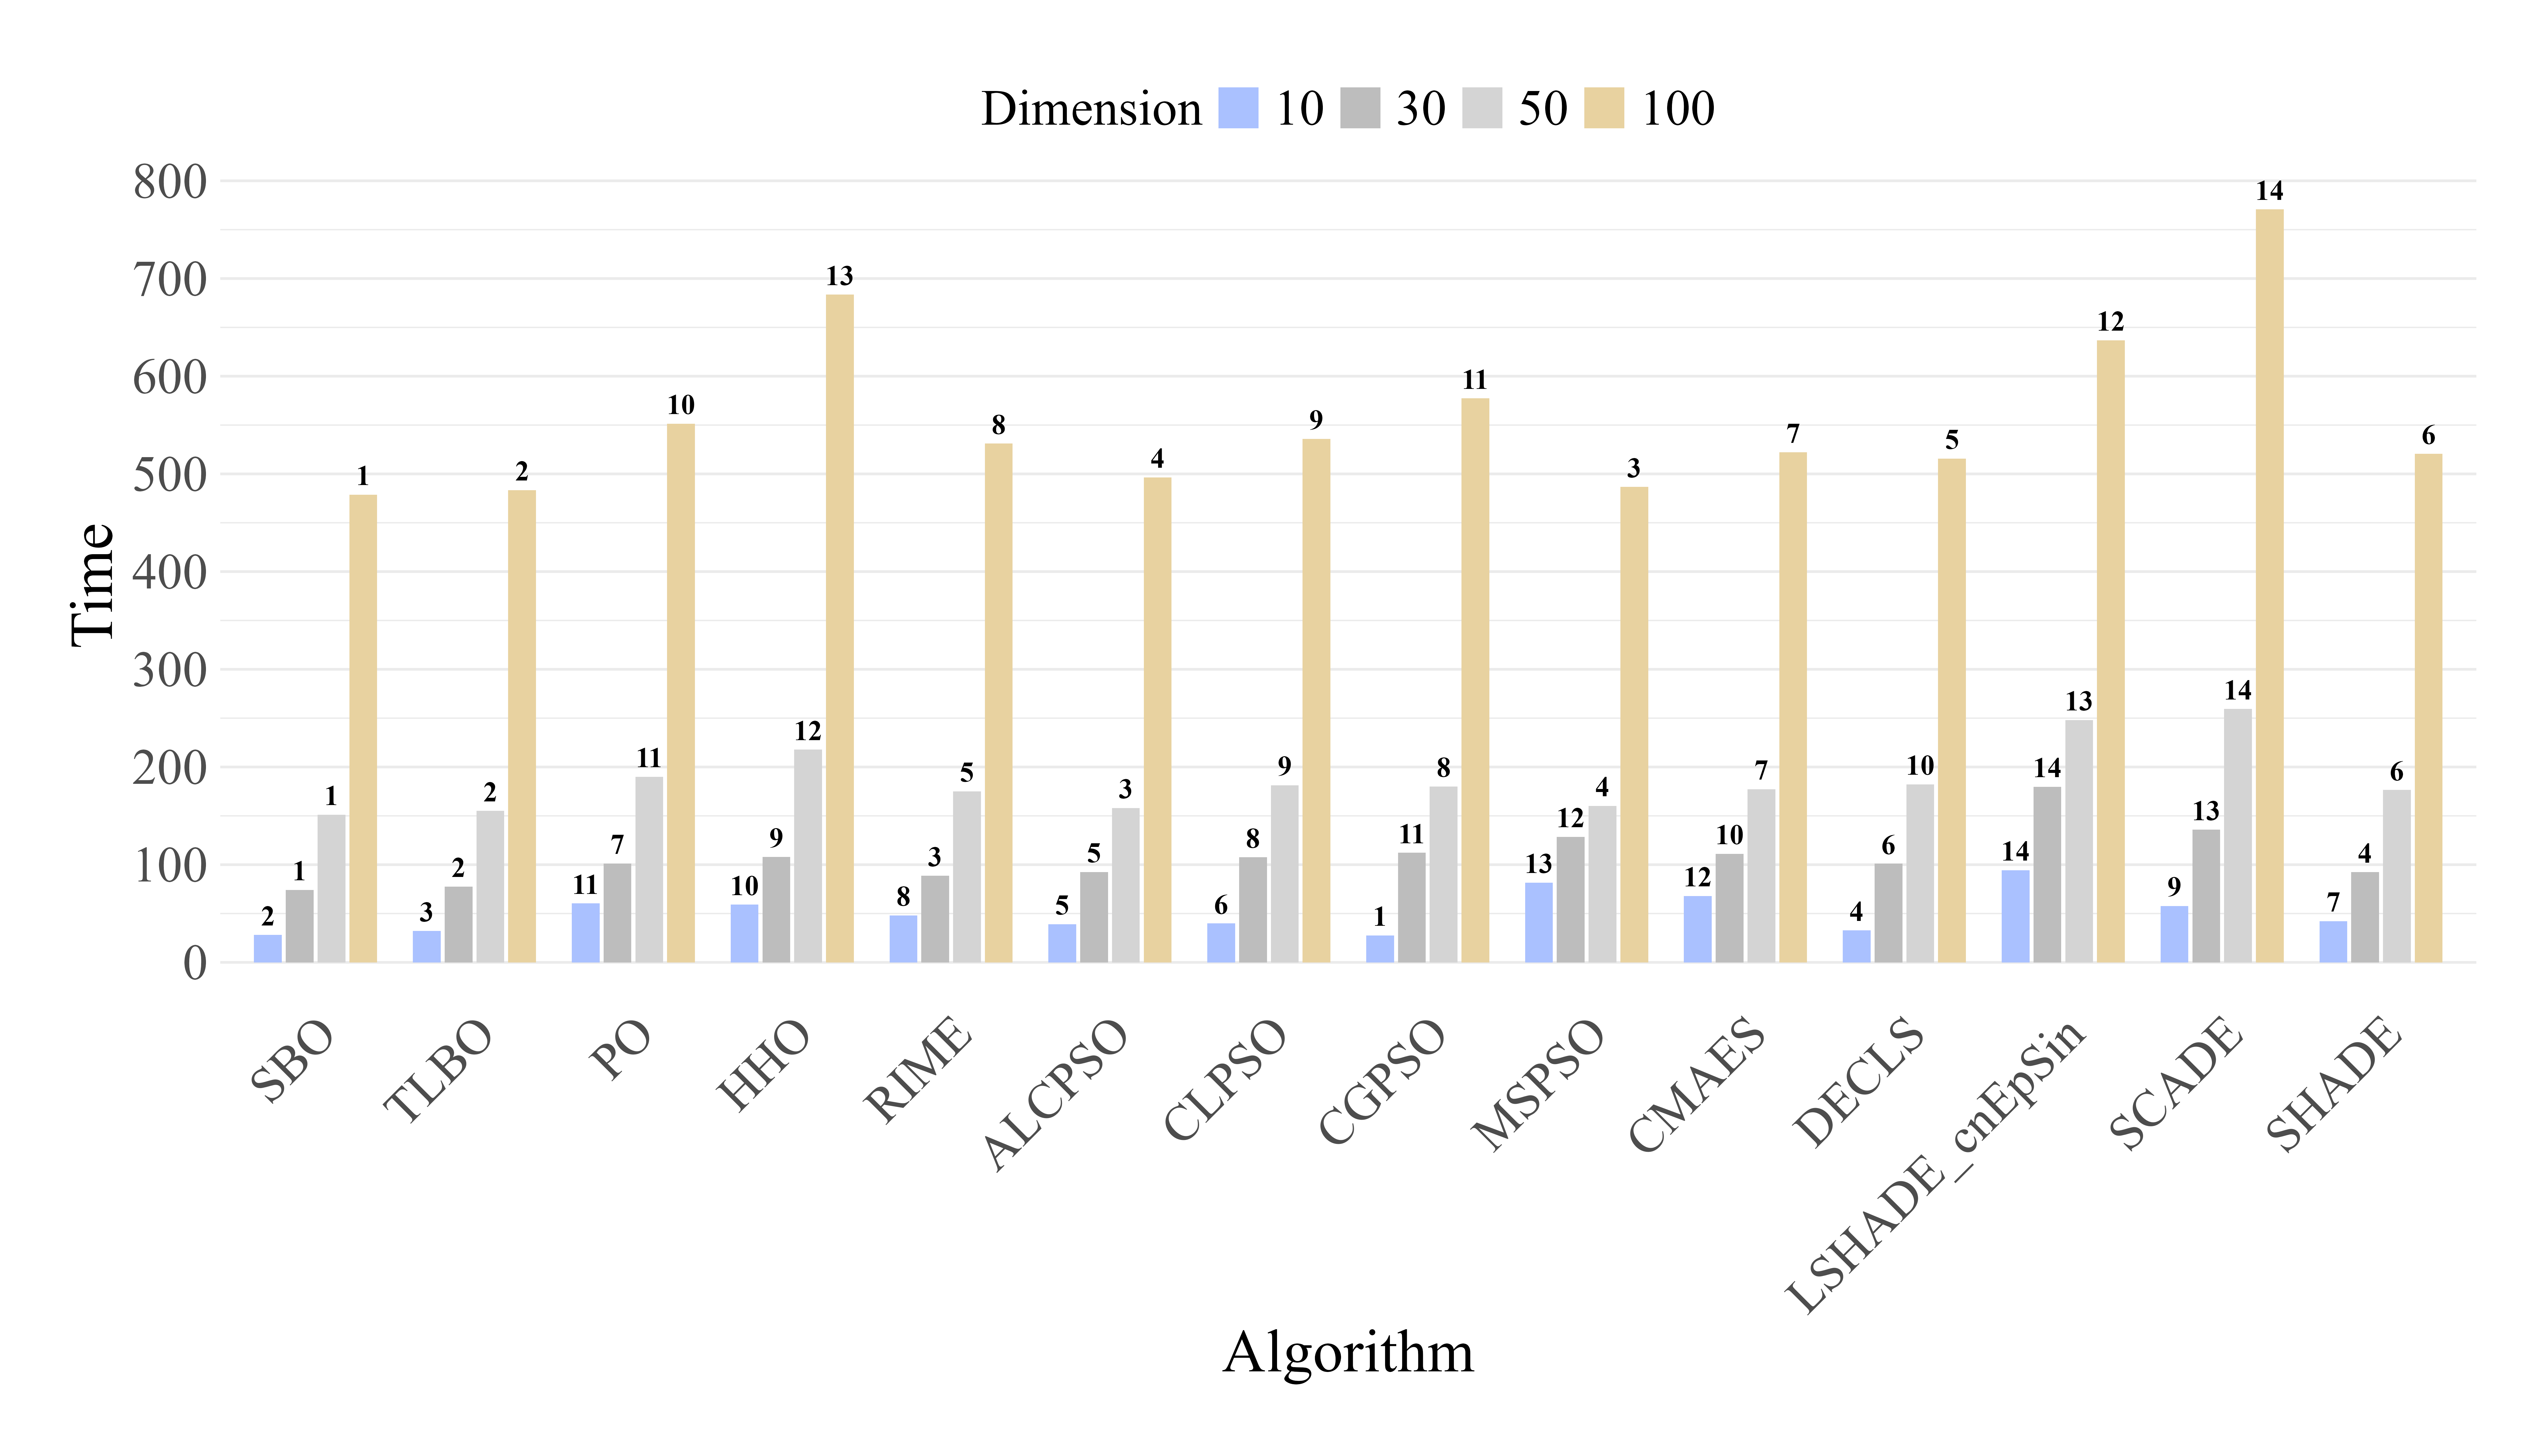
\includegraphics[width=\textwidth]{figures/fig11_runtime_performance.png}
  \caption{Runtime performance of SBO with other algorithms on IEEE CEC 2017.}
  \label{fig:runtime_performance}
\end{figure}




\section{ Experimental Verification}

This section applies the SBO framework to two important optimization applications: feature selection and multi-threshold image segmentation. To solve the classic discrete optimization challenge of feature selection, SBO is converted into its binary variant, bSBO. This adaptation builds upon SBO's demonstrated efficiency in global optimization within continuous spaces, supporting its potential for discrete applications. The bSBO is engineered to optimize feature selection by selecting the most relevant attributes while eliminating redundancy, thereby improving predictive model performance through optimal feature selection. The proposed bSBO is then combined with the KNN classifier to validate performance. Finally, bSBO is benchmarked against 8 state-of-the-art binary optimizers across 9 high-dimensional UCI datasets, proving its competitive advantage in discrete optimization.

Moving beyond feature selection; we also evaluate SBO's performance in multi-threshold image segmentation---a continuous optimization task requiring precise threshold determination for accurate image analysis. For this assessment, SBO competes against 7 advanced meta-heuristic algorithms using 9 breast cancer histology images from Invasive Ductal Carcinoma (IDC) dataset to measure segmentation quality improvements. By maintaining an optimal exploration-exploitation balance, SBO proves highly adaptable across both discrete and continuous problem domains, confirming its versatility for various real-world optimization challenges.




\paragraph{ Feature Selection}

Feature selection is a critical process in dataset analysis that involves picking the most influential and significant features to reduce data dimensionality and omitting redundant and unrelated attributes [61]. This selective extraction not only enhances the generality and robustness of the model trained on these features but also streamlines the computational efficiency. Predominantly, there are three recognized methodologies for feature selection: the filter method [62], the embedded method [63], and the wrapper method [64]---each characterized by distinct selection procedures.

The filter method evaluates feature relevance using statistical metrics, such as the Pearson correlation coefficient [65] for linear feature-target relationships, the Chi-squared test [66] for information gain, and variance thresholding [67] to discard low variance features. These assessments are uniquely machine learning algorithm-independent. In contrast, the embedded method conducts selection intrinsically during the model training phase, integrating feature importance evaluation into the optimization process, with popular techniques including Lasso Regression [68], known as L1 Regularization, which penalizes regression coefficients' absolute value to zero out less significant features, and tree-based methods [69] that automatically determine feature importance. Unlike both approaches, the wrapper method evaluates feature subsets through iterative model training, selecting those that maximize performance based on evaluation metrics, making this method more computationally intensive but often more accurate.

This paper specifically focuses on the bSBO---an MA that iteratively searches for the optimal feature subset, assessed against a fitness-function-based evaluation metric. Given the exponential increase of potential feature combinations with every additional feature, MAs like the proposed bSBO become helpful for managing the combinatorial nature of the feature selection issue, thereby making wrapper-based feature selection an increasingly popular choice in current practices for dataset dimensionality reduction.


\subparagraph{ bSBO-based Wrapper method}

In this section, we present the wrapper-based feature selection method that integrates a KNN classifier (with K set to 5) with the bSBO. A detailed flowchart in Fig. 12 outlines the process for selecting an effective feature subset.

The fitness function is formulated to achieve a trade-off between minimizing the number of selected features and reducing the classifier's error rate. Let $E$ represent the error rate of the KNN classifier, $|S|$ denote the number of features selected by the bSBO, and $|A|$ the total number of features in the dataset. The fitness function is defined in Eq. \left(\mathrm{17}\right). With the parameters set to $α=0.05$ and $β=0.95$, ensuring that more emphasis is placed on the error rate. This formulation guides the optimizer to favor solutions that maintain high predictive accuracy while selecting a compact feature subset.

\begin{tabular}{|p{0.4in}|p{3.1in}|p{0.4in}|} \hline 
 & $f_{obj}=α\times E+β\times \frac{\left|S\right|}{\left|A\right|}$ & $\left(\mathrm{17}\right)$ \\ \hline 
\end{tabular}



The process begins with data preprocessing. The dataset is divided into ten folds and normalized to the range [$\mathrm{-}$1,1]. Each candidate solution is represented as a vector of continuous values, which are then transformed into binary decisions to indicate whether a feature is selected. This conversion is achieved through a V-type transfer function defined as:

\begin{tabular}{|p{0.4in}|p{3.1in}|p{0.4in}|} \hline 
 & $T\left(x_{i,j}\right)=\left|erf\left(sqrt\left(\frac{π}{2}\right)\times x_{i,j}\right)\right|$ & $\left(\mathrm{18}\right)$ \\ \hline 
 & $erf\left(x\right)=\frac{2}{sqrt\left(π\right)}\int^x_0{e^{-t^2}}dt$ & $\left(\mathrm{19}\right)$ \\ \hline 
\end{tabular}

where $x_{i,j}$ is the continuous value of the $jth$ component of the $ith$ candidate solution. The resulting value is then thresholded at 0.5 to yield a binary decision for feature selection.

Following the transformation, each candidate solution corresponds to a binary vector of length $D$, representing the dimensionality of the dataset. The selected feature subset is used to train the KNN classifier on the training data, and its performance is evaluated on the test set to compute the error rate $E$.

The bSBO iteratively updates the candidate solutions over a fixed number of iterations. The fitness function is evaluated at each iteration, and the candidate feature subsets are refined accordingly. Once the optimization process concludes, the best-performing feature subset is used to train the final KNN model, and its predictive accuracy is assessed on the test dataset.

The performance of the bSBO-based approach is evaluated by considering three metrics: the average fitness value across multiple trials, the error rate of the KNN classifier, and the number of features selected. These metrics comprehensively assess the method's ability to achieve both model accuracy and feature reduction. Comparative analysis against eight state-of-the-art binary optimizers further demonstrates the effectiveness of the proposed approach in producing robust and interpretable models.

\noindent 

\begin{figure}[htbp]
  \centering
  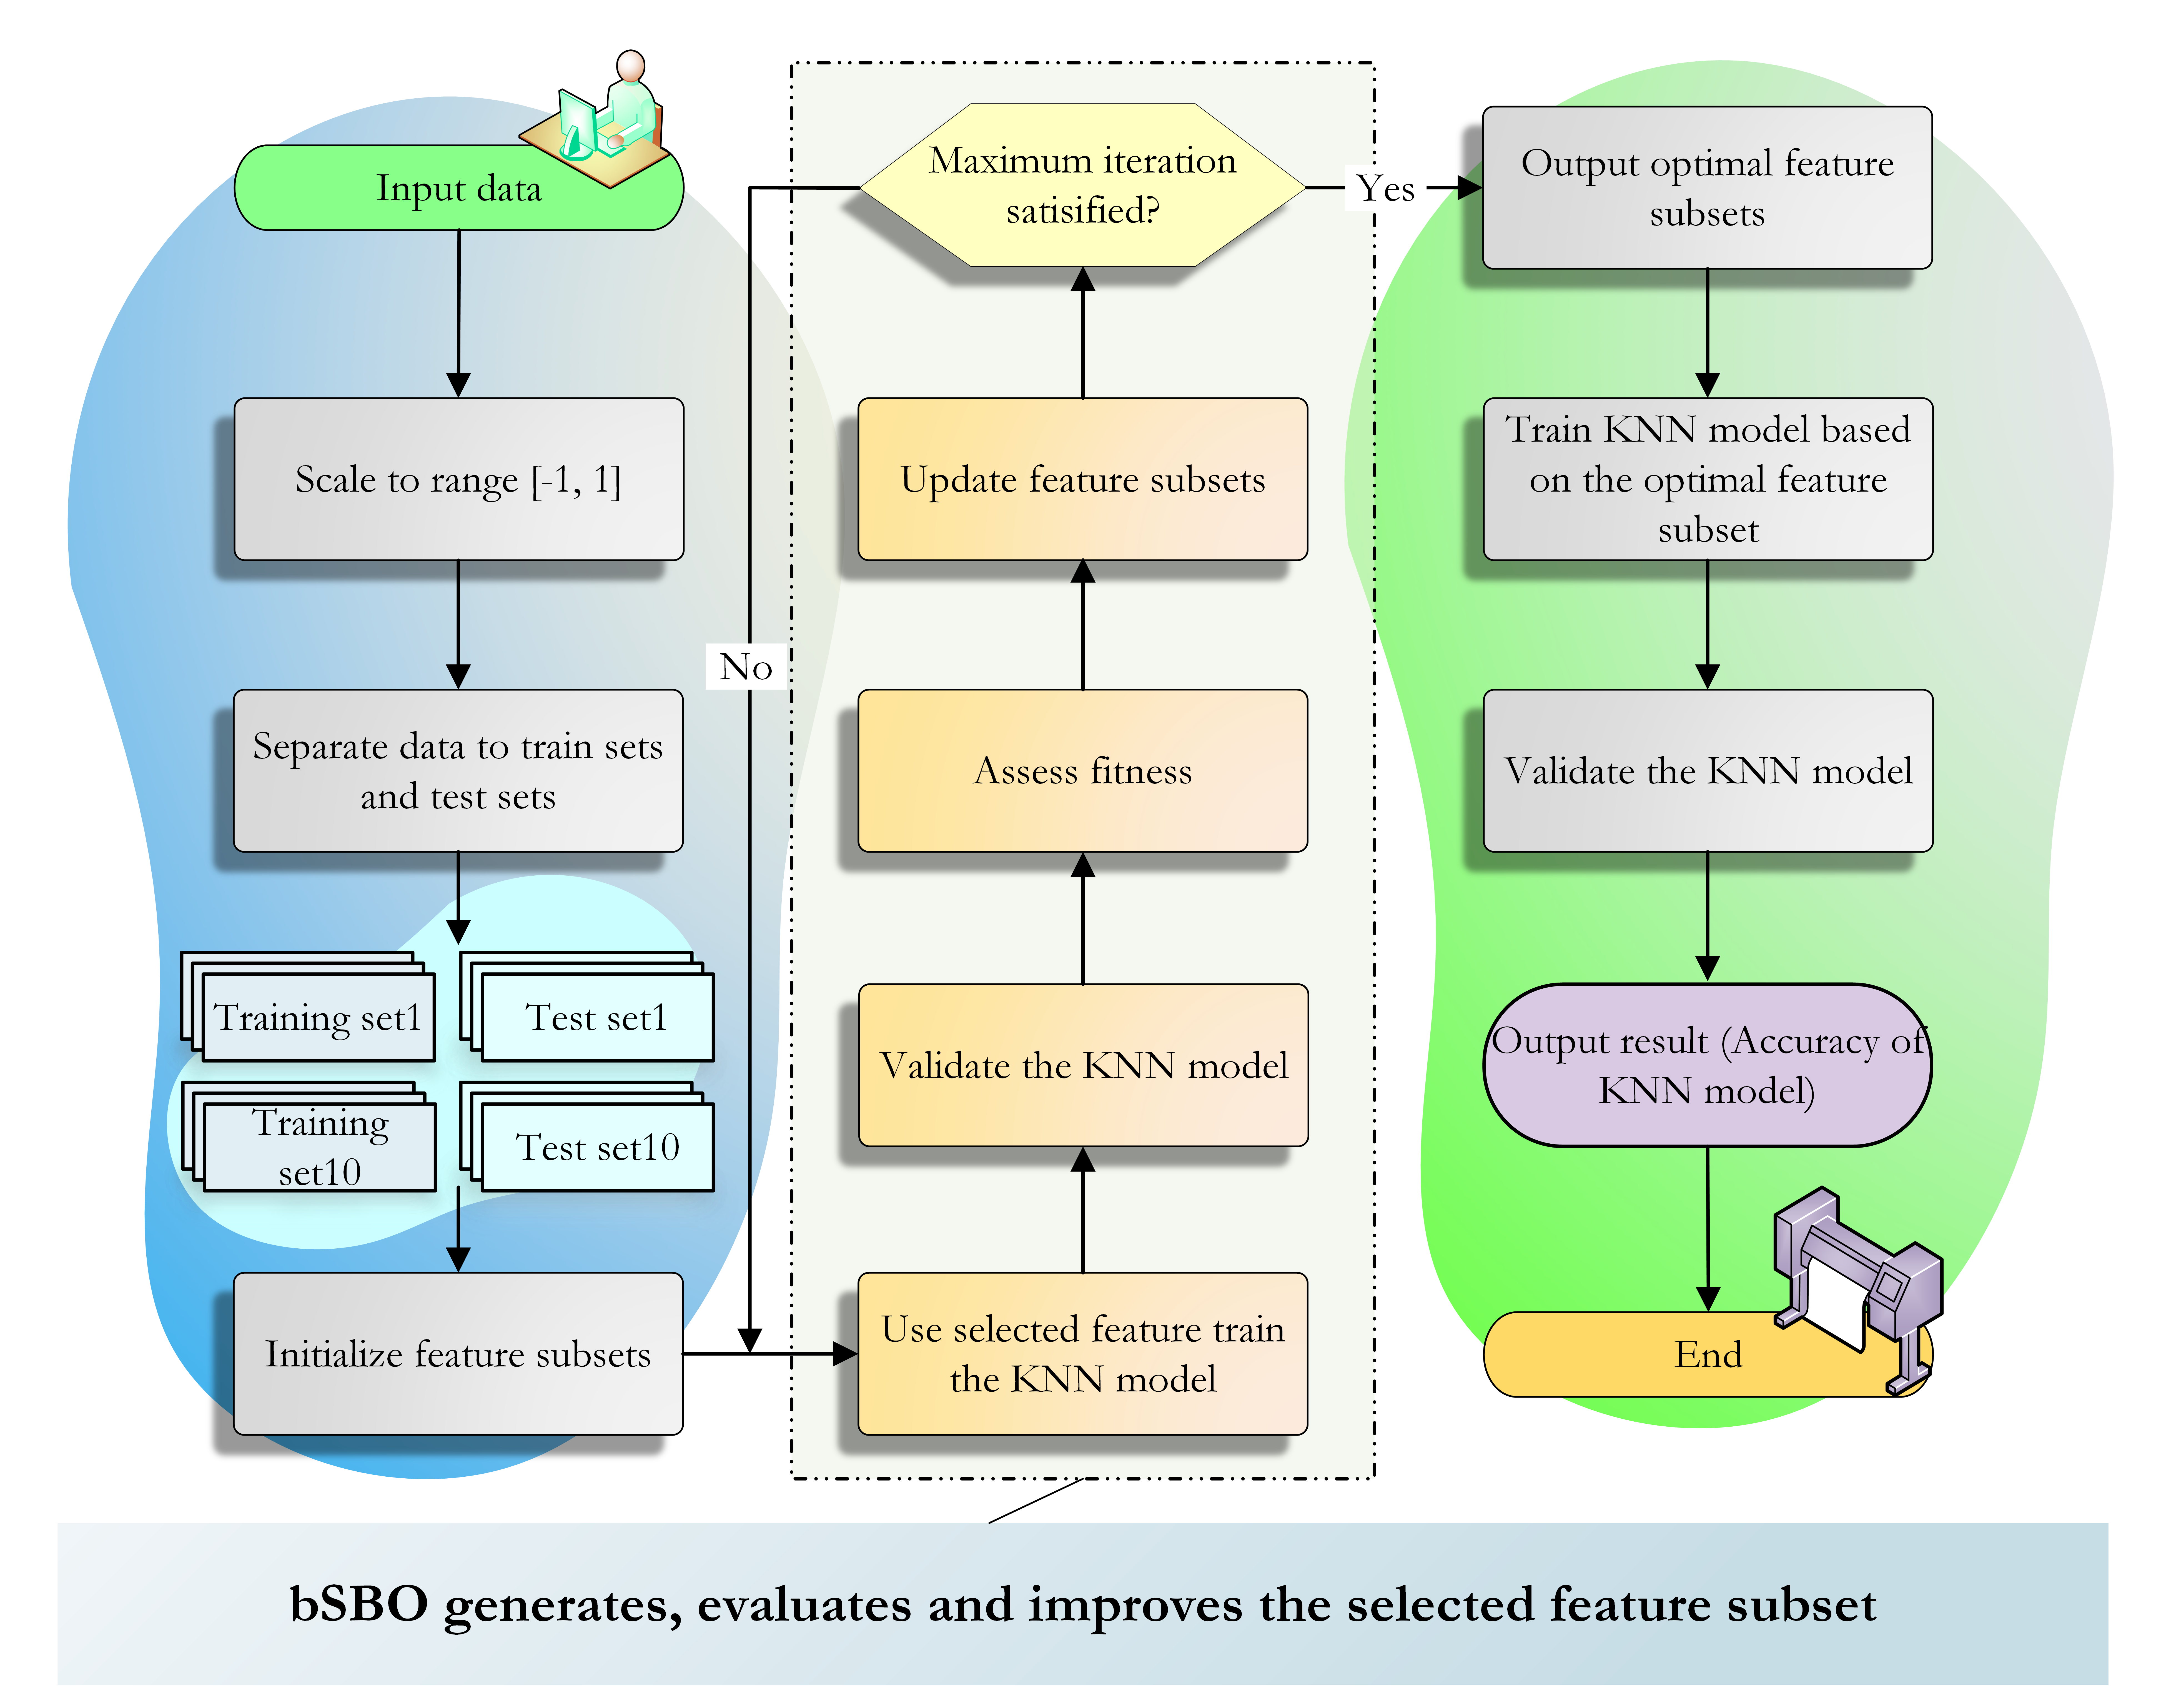
\includegraphics[width=\textwidth]{figures/fig12_flowchart_bSBO_wrapper.png}
  \caption{Flowchart of bSBO-based wrapper method for feature selection.}
  \label{fig:flowchart_bSBO_wrapper}
\end{figure}




\subparagraph{ Experiment results and analysis of bSBO}

This section is dedicated to evaluating the optimization capabilities of bSBO by setting it in direct competition with eight state-of-the-art binary optimizers. These comparators are binary Moth Flame Optimizer (bMFO) [70], bGWO [71], bGSA [72], bPSO [73], binary Ant Lion Optimizer (bALO) [74], binary Bat Algorithm (bBA) [75], binary Salp Swarm Algorithm (bSSA) [76], and bHHO [77]. Each optimizer's control parameters follow their original publications.

The datasets chosen for this comparison are diverse and representative, presented in Table 5 from UCI machine learning repository, with dimensions ranging from 2,308 to 12,600, ensuring comprehensive benchmarking. Additionally, the variation in the number of classes (from two to four) and sample sizes (from 50 to 203 per dataset) provides a robust framework for assessing bSBO's optimization prowess against established binary optimizers across a range of complex data environments.



\begin{tabular}{|p{1.0in}|p{1.0in}|p{1.0in}|p{1.0in}|} \hline 
\multicolumn{4}{|p{1in}|}{\textbf{Table }5\textbf{.} Description of the used high-dimensional datasets.} \\ \hline 
Dataset & Samples & Features & Classes \\ \hline 
Brain\_Tumor2 & 50 & 10367 & 4 \\ \hline 
CNS & 60 & 7129 & 2 \\ \hline 
DLBCL & 77 & 5469 & 2 \\ \hline 
Leukemia & 72 & 7130 & 2 \\ \hline 
Leukemia1 & 72 & 5327 & 3 \\ \hline 
Leukemia2 & 72 & 11225 & 3 \\ \hline 
Lung\_Cancer & 203 & 12600 & 3 \\ \hline 
Prostate\_Tumor & 102 & 10509 & 2 \\ \hline 
SRBCT & 83 & 2308 & 4 \\ \hline 
\end{tabular}



To standardize conditions across all optimized algorithms, the experimental design imposes a termination criterion of 50 maximum iterations and a specified population size of 20. To mitigate the influence of randomness on the results, each optimizer is run 10 times for every dataset. Furthermore, to evaluate the performance of the trained models, a 10-fold cross-validation [78] is employed for each dataset, which is a widely recognized method for ensuring the validity of the machine learning models.

The results of these experiments are presented in Table 6 to Table 8, which provide comparative data on fitness values, the number of features selected, and the error rates for bSBO and the eight other binary optimizers. To quantitatively establish the superiority of bSBO over its counterparts, the results are subjected to statistical analysis employing the Wilcoxon signed-rank test and the Friedman test. These non-parametric tests are chosen for their ability to detect significant differences between paired observations and to compare more than two algorithms over multiple datasets, respectively, providing a robust statistical framework to support the comparative analysis.

Table 6 presents a detailed comparison of fitness values, revealing that bSBO achieves the lowest fitness scores on all nine datasets when compared with the eight other binary optimizers. However, it is important to note certain deviations, specifically the higher Std values for Leukemia2, Lung\_Cancer, and Prostate\_Tumor datasets, where bSBO recorded larger Std values than bHHO, bMFO, and bHHO respectively.

Despite these variances in Std values, the statistical tests presented at the bottom of Table 6 strongly support bSBO's superior performance. It conclusively outperformed the other eight optimizers across all datasets, securing the top rank with a ranking value of 1. This distinctively places bSBO ahead of its closest competitor, bHHO, which achieved a secondary ranking value of 2.25. The inclusion of these statistical tests validates the robustness of bSBO's leading position in optimizing fitness values within the experimented datasets.



\begin{tabular}{|p{0.4in}|p{0.4in}|p{0.4in}|p{0.4in}|p{0.4in}|p{0.4in}|p{0.4in}|p{0.4in}|p{0.4in}|p{0.4in}|p{0.4in}|} \hline 
\multicolumn{11}{|p{1in}|}{\textbf{Table }6\textbf{. }Comparative results of average fitness values between bSBO and other binary optimizers.\textbf{}} \\ \hline 
Dataset & Metric & bSBO & bMFO & bGWO & bGSA & bPSO & bALO & bBA & bSSA & bHHO \\ \hline 
Brain\_Tumor2 & Std & \textbf{3.80E-06} & 1.83E-04 & 6.00E-02 & 1.12E-01 & 1.18E-01 & 9.62E-02 & 2.30E-01 & 8.49E-02 & 8.82E-02 \\ \hline 
 & Avg & \textbf{9.65E-06} & 1.71E-04 & 5.74E-03 & 1.02E-01 & 2.39E-02 & 2.37E-02 & 2.04E-02 & 1.95E-02 & 9.27E-03 \\ \hline 
CNS & Std & \textbf{2.25E-05} & 2.25E-04 & 6.67E-02 & 7.91E-02 & 1.09E-01 & 8.34E-02 & 1.48E-01 & 1.31E-01 & 1.23E-04 \\ \hline 
 & Avg & \textbf{1.75E-05} & 2.77E-04 & 5.86E-03 & 2.32E-02 & 1.82E-01 & 1.70E-01 & 2.37E-01 & 1.04E-01 & 4.21E-05 \\ \hline 
DLBCL & Std & \textbf{7.21E-06} & 1.08E-04 & 2.80E-04 & 3.77E-02 & 3.75E-02 & 3.28E-04 & 3.70E-02 & 4.41E-02 & 1.88E-05 \\ \hline 
 & Avg & \textbf{1.83E-05} & 1.14E-04 & 5.33E-03 & 2.16E-02 & 2.34E-02 & 2.29E-02 & 2.14E-02 & 2.23E-03 & \textbf{1.83E-05} \\ \hline 
Leukemia & Std & \textbf{5.73E-06} & 6.30E-05 & 2.55E-04 & 1.97E-04 & 2.49E-04 & 2.12E-04 & 3.22E-03 & 8.97E-03 & 1.85E-05 \\ \hline 
 & Avg & \textbf{1.40E-05} & 7.71E-05 & 5.49E-03 & 2.18E-02 & 2.34E-02 & 2.30E-02 & 1.65E-02 & 2.40E-02 & 1.75E-05 \\ \hline 
Leukemia1 & Std & \textbf{6.07E-05} & 1.86E-04 & 3.53E-04 & 3.55E-04 & 2.06E-04 & 2.32E-04 & 4.23E-02 & 6.53E-03 & 1.06E-04 \\ \hline 
 & Avg & \textbf{1.88E-05} & 1.88E-04 & 5.28E-03 & 2.14E-02 & 2.31E-02 & 2.27E-02 & 1.79E-02 & 2.30E-02 & 5.16E-05 \\ \hline 
Leukemia2 & Std & 2.44E-05 & 8.46E-05 & 1.76E-04 & 3.60E-04 & 5.38E-02 & 5.38E-02 & 6.16E-02 & 5.90E-02 & \textbf{2.27E-05} \\ \hline 
 & Avg & \textbf{1.78E-05} & 1.45E-04 & 5.43E-03 & 2.25E-02 & 2.37E-02 & 2.35E-02 & 1.76E-02 & 2.42E-02 & 3.12E-05 \\ \hline 
Lung\_Cancer & Std & 4.02E-04 & \textbf{3.11E-04} & 2.11E-02 & 3.41E-02 & 3.41E-02 & 2.23E-02 & 4.27E-02 & 3.13E-02 & 2.30E-02 \\ \hline 
 & Avg & \textbf{8.13E-05} & 5.58E-04 & 6.01E-03 & 4.45E-02 & 4.68E-02 & 2.39E-02 & 4.29E-02 & 3.86E-02 & 8.64E-03 \\ \hline 
Prostate\_Tumor & Std & 6.37E-05 & 1.89E-04 & 2.99E-02 & 4.80E-02 & 7.66E-02 & 4.80E-02 & 9.69E-02 & 5.15E-02 & \textbf{5.22E-05} \\ \hline 
 & Avg & \textbf{2.62E-05} & 2.47E-04 & 6.19E-03 & 2.30E-02 & 2.42E-02 & 2.38E-02 & 1.11E-01 & 6.77E-02 & 7.14E-05 \\ \hline 
SRBCT & Std & \textbf{7.81E-05} & 1.04E-04 & 2.85E-04 & 4.19E-04 & 3.74E-02 & 3.50E-04 & 4.82E-02 & 4.93E-02 & 1.50E-04 \\ \hline 
\textbf{} & Avg & \textbf{1.08E-04} & 1.95E-04 & 4.15E-03 & 1.95E-02 & 2.22E-02 & 2.16E-02 & 1.73E-02 & 2.24E-02 & 1.19E-04 \\ \hline 
\textbf{+/-/=} & $\mathrm{\sim}$ & $\mathrm{\sim}$ & 9/0/0 & 9/0/0 & 9/0/0 & 9/0/0 & 9/0/0 & 9/0/0 & 9/0/0 & 8/1/0 \\ \hline 
Friedman-rank &  & 1.00  & 2.88  & 3.88  & 5.88  & 7.88  & 6.63  & 8.38  & 6.25  & 2.25  \\ \hline 
Result &  & 1 & 3 & 4 & 5 & 8 & 7 & 9 & 6 & 2 \\ \hline 
\end{tabular}



Table 7 and Table 8 show the results regarding the number of selected features and the corresponding error rates of the machine learning models trained with those features. These tables also feature the non-parametric statistical results at the bottom for a thorough analytical insight. The findings indicate that bSBO not only selects the minimal number of features but also accomplishes the lowest error rates across the nine datasets. According to the rankings for both the number of selected features and the error rates, bSBO consistently achieves the top position with a rank of 1.

In Table 7, there are observations of larger Std values corresponding to the Leukemia2, Lung\_Cancer, and Prostate\_Tumor datasets, but the small difference in Std values when comparing bSBO with bHHO, bGSA, and bHHO respectively underscores the consistency and robustness of bSBO.

For enhanced visual interpretation and comparative analysis of bSBO's robust performance against other optimizers, Fig. 13 presents the Friedman rank results using a bar plot. This visualization clearly depicts the relative performance of different optimizers across multiple evaluation metrics. Lower ranks indicate better performance, with bSBO achieving the most favorable rankings and thereby demonstrating its consistent superiority.



\begin{tabular}{|p{0.4in}|p{0.4in}|p{0.4in}|p{0.4in}|p{0.4in}|p{0.4in}|p{0.4in}|p{0.4in}|p{0.4in}|p{0.4in}|p{0.4in}|} \hline 
\multicolumn{11}{|p{1in}|}{\textbf{Table }7\textbf{. }Comparative results of average selected feature numbers between bSBO and other binary optimizers.\textbf{}} \\ \hline 
Dataset & Metric & bSBO & bMFO & bGWO & bGSA & bPSO & bALO & bBA & bSSA & bHHO \\ \hline 
Brain\_Tumor2 & Std & \textbf{7.89E-01} & 3.80E+01 & 4.77E+01 & 5.66E+01 & 7.97E+01 & 5.94E+01 & 2.28E+02 & 2.21E+03 & 6.36E+02 \\ \hline 
 & Avg & \textbf{2.00E+00} & 3.55E+01 & 1.17E+03 & 4.67E+03 & 4.93E+03 & 4.89E+03 & 4.15E+03 & 2.90E+03 & 1.25E+03 \\ \hline 
CNS & Std & \textbf{3.21E+00} & 3.21E+01 & 4.09E+01 & 6.98E+01 & 4.78E+01 & 4.93E+01 & 2.45E+02 & 1.25E+03 & 1.76E+01 \\ \hline 
 & Avg & \textbf{2.50E+00} & 3.95E+01 & 8.35E+02 & 3.23E+03 & 3.39E+03 & 3.33E+03 & 2.89E+03 & 3.49E+03 & 6.00E+00 \\ \hline 
DLBCL & Std & \textbf{7.89E-01} & 1.18E+01 & 3.06E+01 & 3.84E+01 & 2.29E+01 & 3.59E+01 & 1.44E+02 & 1.20E+03 & 2.06E+00 \\ \hline 
 & Avg & \textbf{2.00E+00} & 1.25E+01 & 5.83E+02 & 2.36E+03 & 2.56E+03 & 2.50E+03 & 2.28E+03 & 2.44E+02 & \textbf{2.00E+00} \\ \hline 
Leukemia & Std & \textbf{8.17E-01} & 8.99E+00 & 3.63E+01 & 2.81E+01 & 3.55E+01 & 3.02E+01 & 1.46E+02 & 1.28E+03 & 2.63E+00 \\ \hline 
 & Avg & \textbf{2.00E+00} & 1.10E+01 & 7.83E+02 & 3.11E+03 & 3.34E+03 & 3.28E+03 & 2.88E+03 & 3.42E+03 & 2.50E+00 \\ \hline 
Leukemia1 & Std & \textbf{6.47E+00} & 1.98E+01 & 3.76E+01 & 3.78E+01 & 2.19E+01 & 2.47E+01 & 7.35E+01 & 6.96E+02 & 1.13E+01 \\ \hline 
 & Avg & \textbf{2.00E+00} & 2.00E+01 & 5.62E+02 & 2.28E+03 & 2.47E+03 & 2.42E+03 & 2.20E+03 & 2.45E+03 & 5.50E+00 \\ \hline 
Leukemia2 & Std & 5.48E+00 & 1.90E+01 & 3.94E+01 & 8.07E+01 & 3.66E+01 & 3.76E+01 & 6.39E+02 & 1.97E+03 & \textbf{5.09E+00} \\ \hline 
 & Avg & \textbf{4.00E+00} & 3.25E+01 & 1.22E+03 & 5.04E+03 & 5.32E+03 & 5.27E+03 & 4.48E+03 & 5.39E+03 & 7.00E+00 \\ \hline 
Lung\_Cancer & Std & 1.01E+02 & 7.84E+01 & 8.37E+01 & \textbf{2.77E+01} & 5.77E+01 & 7.66E+01 & 2.72E+02 & 2.37E+03 & 2.85E+02 \\ \hline 
 & Avg & \textbf{2.05E+01} & 1.41E+02 & 1.51E+03 & 5.74E+03 & 6.04E+03 & 5.97E+03 & 5.11E+03 & 4.85E+03 & 1.96E+03 \\ \hline 
Prostate\_Tumor & Std & 1.34E+01 & 3.97E+01 & 6.06E+01 & 6.86E+01 & 3.51E+01 & 4.59E+01 & 2.26E+02 & 1.58E+03 & \textbf{1.10E+01} \\ \hline 
 & Avg & \textbf{5.50E+00} & 5.20E+01 & 1.28E+03 & 4.74E+03 & 5.07E+03 & 4.98E+03 & 4.26E+03 & 5.15E+03 & 1.50E+01 \\ \hline 
SRBCT & Std & \textbf{3.60E+00} & 4.78E+00 & 1.32E+01 & 1.94E+01 & 1.73E+01 & 1.62E+01 & 4.66E+01 & 2.05E+02 & 6.93E+00 \\ \hline 
\textbf{} & Avg & \textbf{5.00E+00} & 9.00E+00 & 1.92E+02 & 8.99E+02 & 1.02E+03 & 9.97E+02 & 9.22E+02 & 1.03E+03 & 5.50E+00 \\ \hline 
\textbf{+/-/=} & $\mathrm{\sim}$ & $\mathrm{\sim}$ & 9/0/0 & 9/0/0 & 9/0/0 & 9/0/0 & 9/0/0 & 9/0/0 & 9/0/0 & 8/1/0 \\ \hline 
Friedman-rank &  & 1.00  & 2.88  & 3.88  & 6.75  & 9.00  & 8.00  & 6.00  & 5.25  & 2.25  \\ \hline 
Result &  & 1 & 3 & 4 & 7 & 9 & 8 & 6 & 5 & 2 \\ \hline 
\end{tabular}



\begin{tabular}{|p{0.4in}|p{0.4in}|p{0.4in}|p{0.4in}|p{0.4in}|p{0.4in}|p{0.4in}|p{0.4in}|p{0.4in}|p{0.4in}|p{0.4in}|} \hline 
\multicolumn{11}{|p{1in}|}{\textbf{Table }8\textbf{.} Comparative results of average error rates between bSBO and other binary optimizers.\textbf{}} \\ \hline 
Dataset & Metric & bSBO & bMFO & bGWO & bGSA & bPSO & bALO & bBA & bSSA & bHHO \\ \hline 
Brain\_Tumor2 & Std & \textbf{0.00E+00} & \textbf{0.00E+00} & 6.32E-02 & 1.18E-01 & 1.25E-01 & 1.01E-01 & 2.97E-01 & 8.31E-02 & 9.39E-02 \\ \hline 
 & Avg & \textbf{0.00E+00} & \textbf{0.00E+00} & \textbf{0.00E+00} & 8.33E-02 & \textbf{0.00E+00} & \textbf{0.00E+00} & 2.25E-01 & \textbf{0.00E+00} & \textbf{0.00E+00} \\ \hline 
CNS & Std & \textbf{0.00E+00} & \textbf{0.00E+00} & 7.03E-02 & 8.33E-02 & 1.15E-01 & 8.79E-02 & 1.07E-01 & 1.39E-01 & \textbf{0.00E+00} \\ \hline 
 & Avg & \textbf{0.00E+00} & \textbf{0.00E+00} & \textbf{0.00E+00} & \textbf{0.00E+00} & 1.67E-01 & 1.55E-01 & 3.33E-01 & 8.33E-02 & \textbf{0.00E+00} \\ \hline 
DLBCL & Std & \textbf{0.00E+00} & \textbf{0.00E+00} & \textbf{0.00E+00} & 3.95E-02 & 3.95E-02 & \textbf{0.00E+00} & 9.71E-02 & 3.95E-02 & \textbf{0.00E+00} \\ \hline 
 & Avg & \textbf{0.00E+00} & \textbf{0.00E+00} & \textbf{0.00E+00} & \textbf{0.00E+00} & \textbf{0.00E+00} & \textbf{0.00E+00} & \textbf{0.00E+00} & \textbf{0.00E+00} & \textbf{0.00E+00} \\ \hline 
Leukemia & Std & \textbf{0.00E+00} & \textbf{0.00E+00} & \textbf{0.00E+00} & \textbf{0.00E+00} & \textbf{0.00E+00} & \textbf{0.00E+00} & 7.17E-02 & \textbf{0.00E+00} & \textbf{0.00E+00} \\ \hline 
 & Avg & \textbf{0.00E+00} & \textbf{0.00E+00} & \textbf{0.00E+00} & \textbf{0.00E+00} & \textbf{0.00E+00} & \textbf{0.00E+00} & \textbf{0.00E+00} & \textbf{0.00E+00} & \textbf{0.00E+00} \\ \hline 
Leukemia1 & Std & \textbf{0.00E+00} & \textbf{0.00E+00} & \textbf{0.00E+00} & \textbf{0.00E+00} & \textbf{0.00E+00} & \textbf{0.00E+00} & 8.31E-02 & \textbf{0.00E+00} & \textbf{0.00E+00} \\ \hline 
 & Avg & \textbf{0.00E+00} & \textbf{0.00E+00} & \textbf{0.00E+00} & \textbf{0.00E+00} & \textbf{0.00E+00} & \textbf{0.00E+00} & 7.14E-02 & \textbf{0.00E+00} & \textbf{0.00E+00} \\ \hline 
Leukemia2 & Std & \textbf{0.00E+00} & \textbf{0.00E+00} & \textbf{0.00E+00} & \textbf{0.00E+00} & 5.66E-02 & 5.66E-02 & 1.16E-01 & 6.02E-02 & \textbf{0.00E+00} \\ \hline 
 & Avg & \textbf{0.00E+00} & \textbf{0.00E+00} & \textbf{0.00E+00} & \textbf{0.00E+00} & \textbf{0.00E+00} & \textbf{0.00E+00} & \textbf{0.00E+00} & \textbf{0.00E+00} & \textbf{0.00E+00} \\ \hline 
Lung\_Cancer & Std & \textbf{0.00E+00} & \textbf{0.00E+00} & 2.22E-02 & 3.59E-02 & 3.60E-02 & 2.34E-02 & 5.18E-02 & 4.03E-02 & 2.42E-02 \\ \hline 
 & Avg & \textbf{0.00E+00} & \textbf{0.00E+00} & \textbf{0.00E+00} & 2.27E-02 & 2.38E-02 & \textbf{0.00E+00} & 9.52E-02 & 2.38E-02 & \textbf{0.00E+00} \\ \hline 
Prostate\_Tumor & Std & \textbf{0.00E+00} & \textbf{0.00E+00} & 3.16E-02 & 5.05E-02 & 8.06E-02 & 5.05E-02 & 1.27E-01 & 5.09E-02 & \textbf{0.00E+00} \\ \hline 
 & Avg & \textbf{0.00E+00} & \textbf{0.00E+00} & \textbf{0.00E+00} & \textbf{0.00E+00} & \textbf{0.00E+00} & \textbf{0.00E+00} & 2.50E-01 & 4.55E-02 & \textbf{0.00E+00} \\ \hline 
SRBCT & Std & \textbf{0.00E+00} & \textbf{0.00E+00} & \textbf{0.00E+00} & \textbf{0.00E+00} & 3.95E-02 & \textbf{0.00E+00} & 5.95E-02 & 4.99E-02 & \textbf{0.00E+00} \\ \hline 
\textbf{} & Avg & \textbf{0.00E+00} & \textbf{0.00E+00} & \textbf{0.00E+00} & \textbf{0.00E+00} & \textbf{0.00E+00} & \textbf{0.00E+00} & 1.11E-01 & \textbf{0.00E+00} & \textbf{0.00E+00} \\ \hline 
\textbf{+/-/=} & $\mathrm{\sim}$ & $\mathrm{\sim}$ & 1/8/0 & 5/4/0 & 5/4/0 & 7/2/0 & 5/4/0 & 8/1/0 & 7/2/0 & 2/7/0 \\ \hline 
Friedman-rank &  & 1.00  & 1.13  & 2.50  & 3.88  & 6.13  & 4.25  & 9.00  & 5.88  & 1.63  \\ \hline 
Result &  & 1 & 2 & 4 & 5 & 8 & 6 & 9 & 7 & 3 \\ \hline 
\end{tabular}



\begin{figure}[htbp]
  \centering
  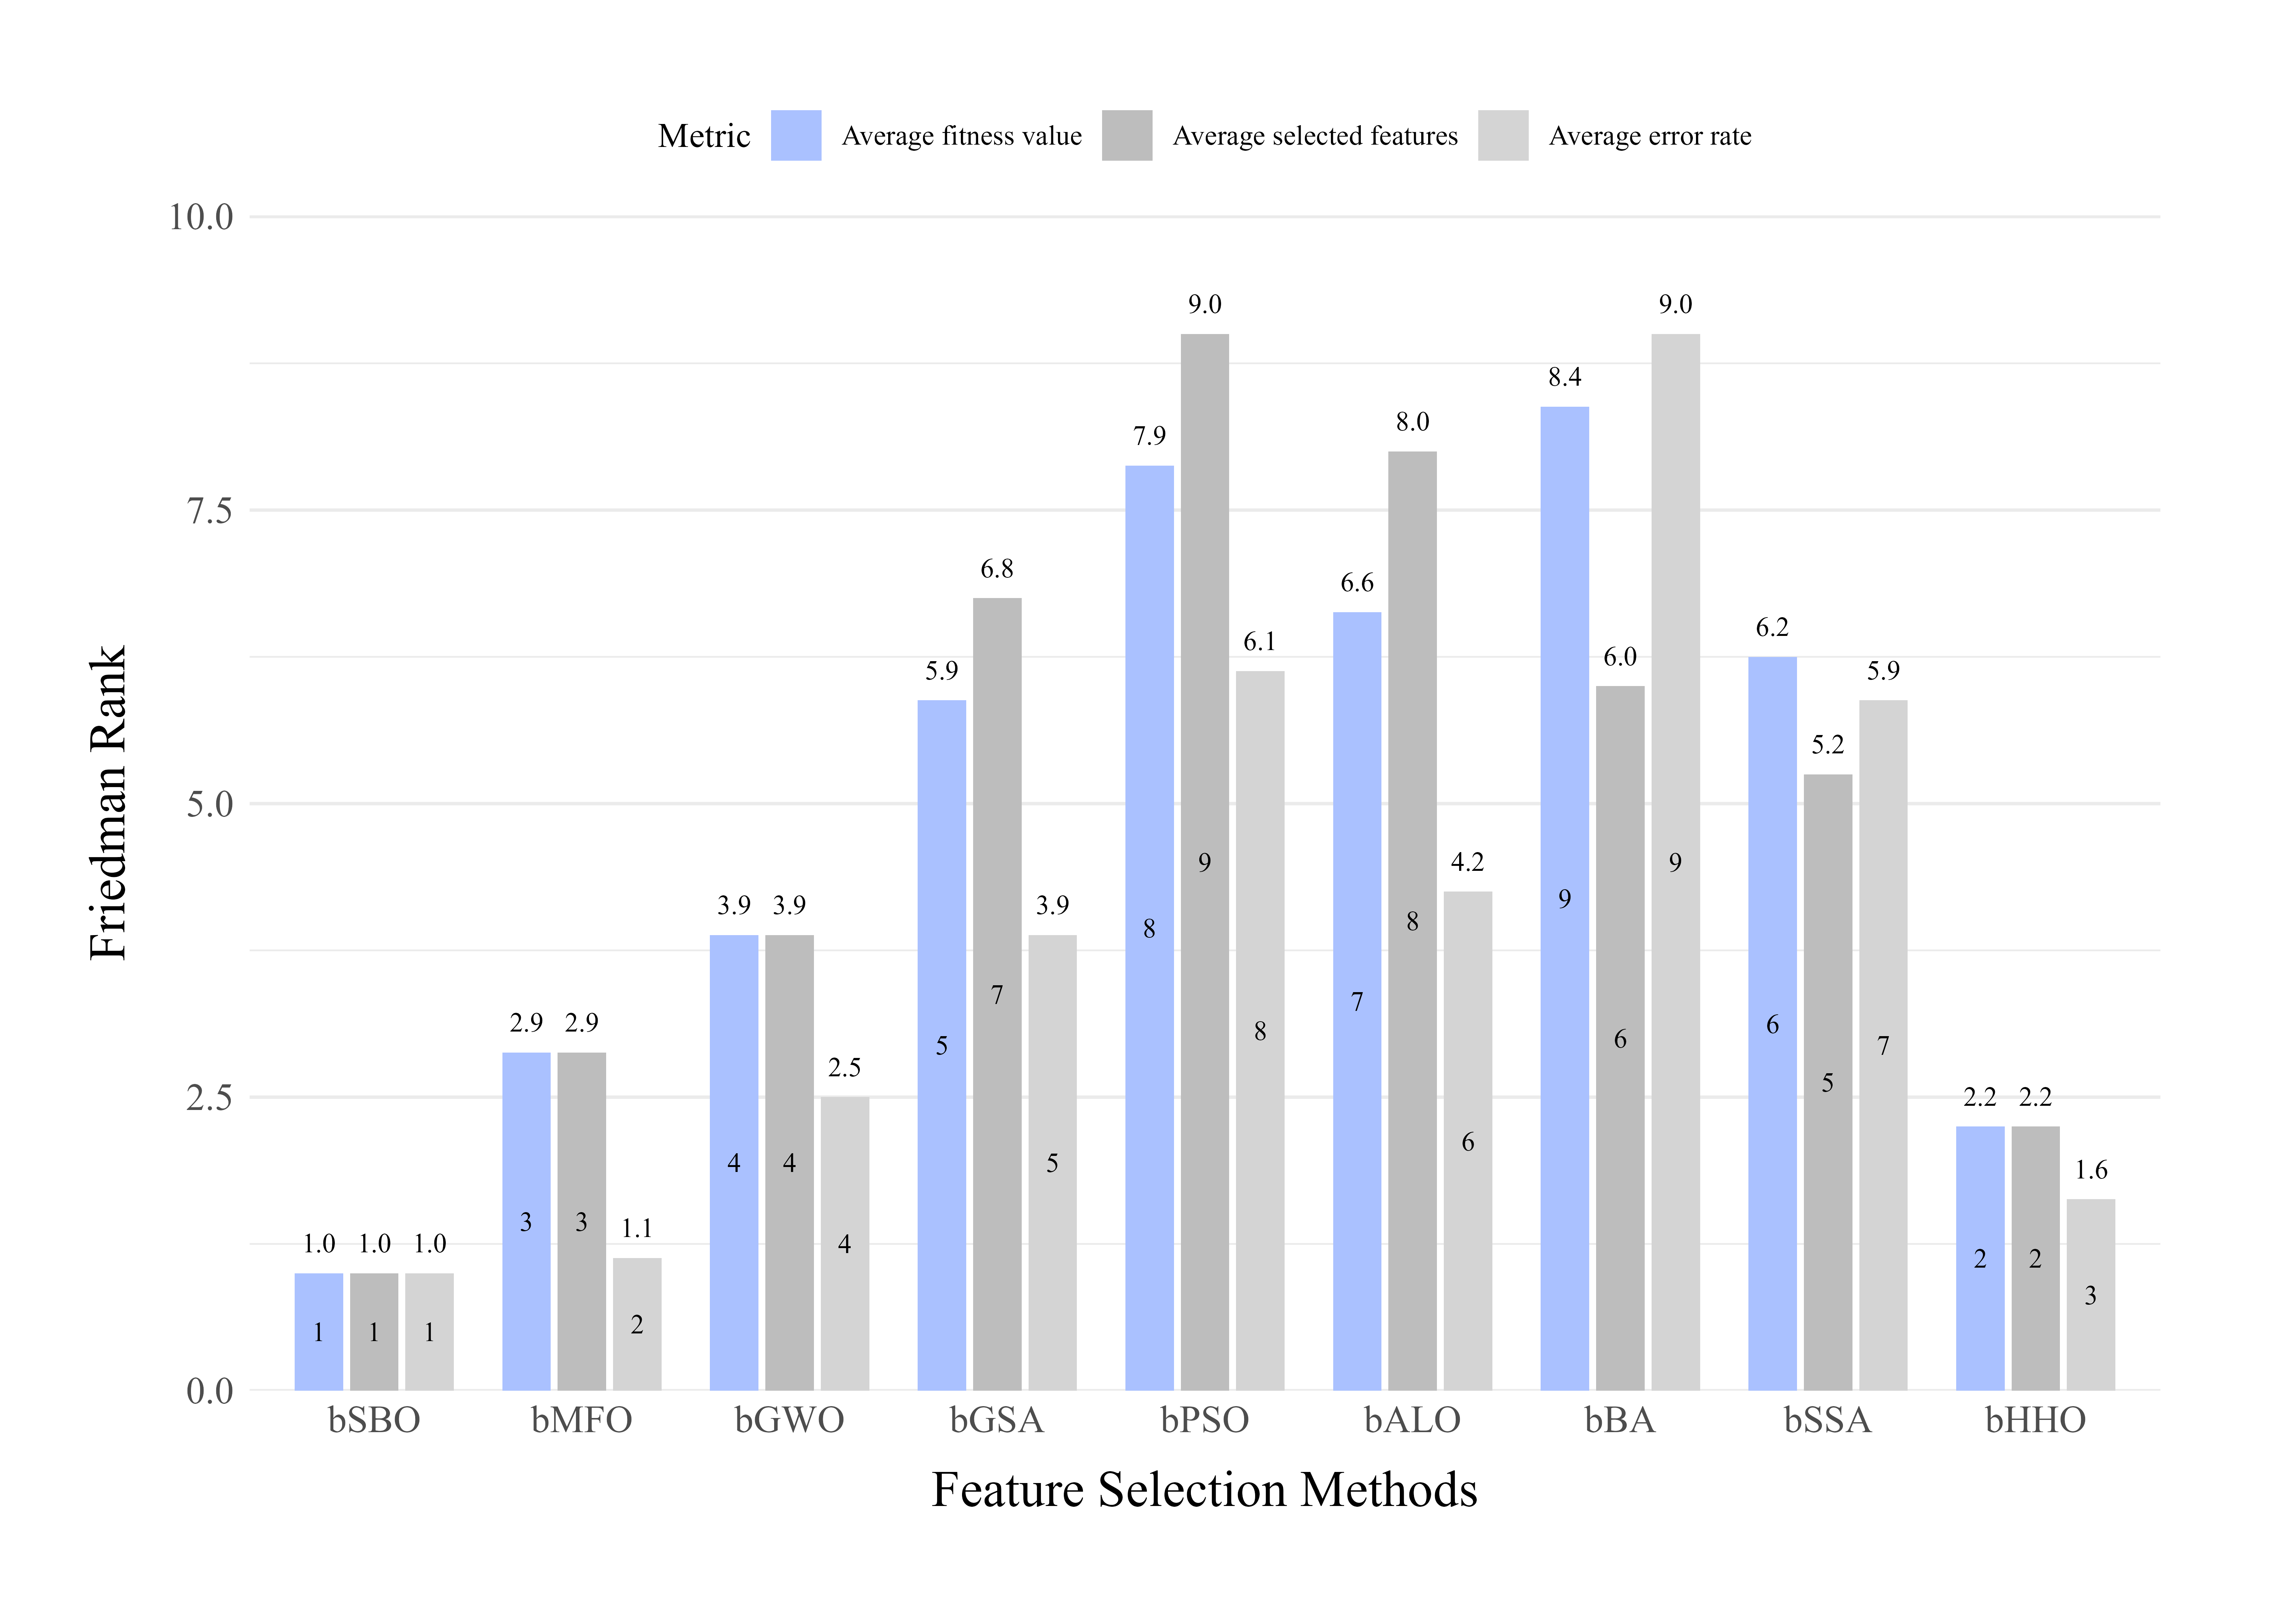
\includegraphics[width=\textwidth]{figures/fig13_friedman_rank_feature_selection.png}
  \caption{Friedman rank results over three metrics.}
  \label{fig:friedman_rank_feature_selection}
\end{figure}



In contrast, other optimizers show greater rank fluctuations, reflecting performance inconsistencies across different evaluation criteria. Notably, bSSA exhibits significant rank variability, suggesting a lack of robustness compared to bSBO. The bar plot effectively illustrates these differences, thereby underscoring the stability and overall superior performance of bSBO among the evaluated optimizers.

Fig. 14 illustrates the convergence curves for each optimizer over multiple iterations, showing the progression toward optimal fitness values on each dataset. The curves indicate that bSBO reaches the optimal fitness values across all nine datasets faster than the other optimizers, particularly within the first 50 iterations. This suggests that while other optimizers may experience early stagnation, bSBO continues to identify superior feature subsets efficiently. Specifically, for the Prostate\_Tumor dataset, bHHO demonstrates competitive performance relative to bSBO. A closer examination reveals subtle advantages of bSBO that may not be immediately apparent.

\begin{figure}[htbp]
  \centering
  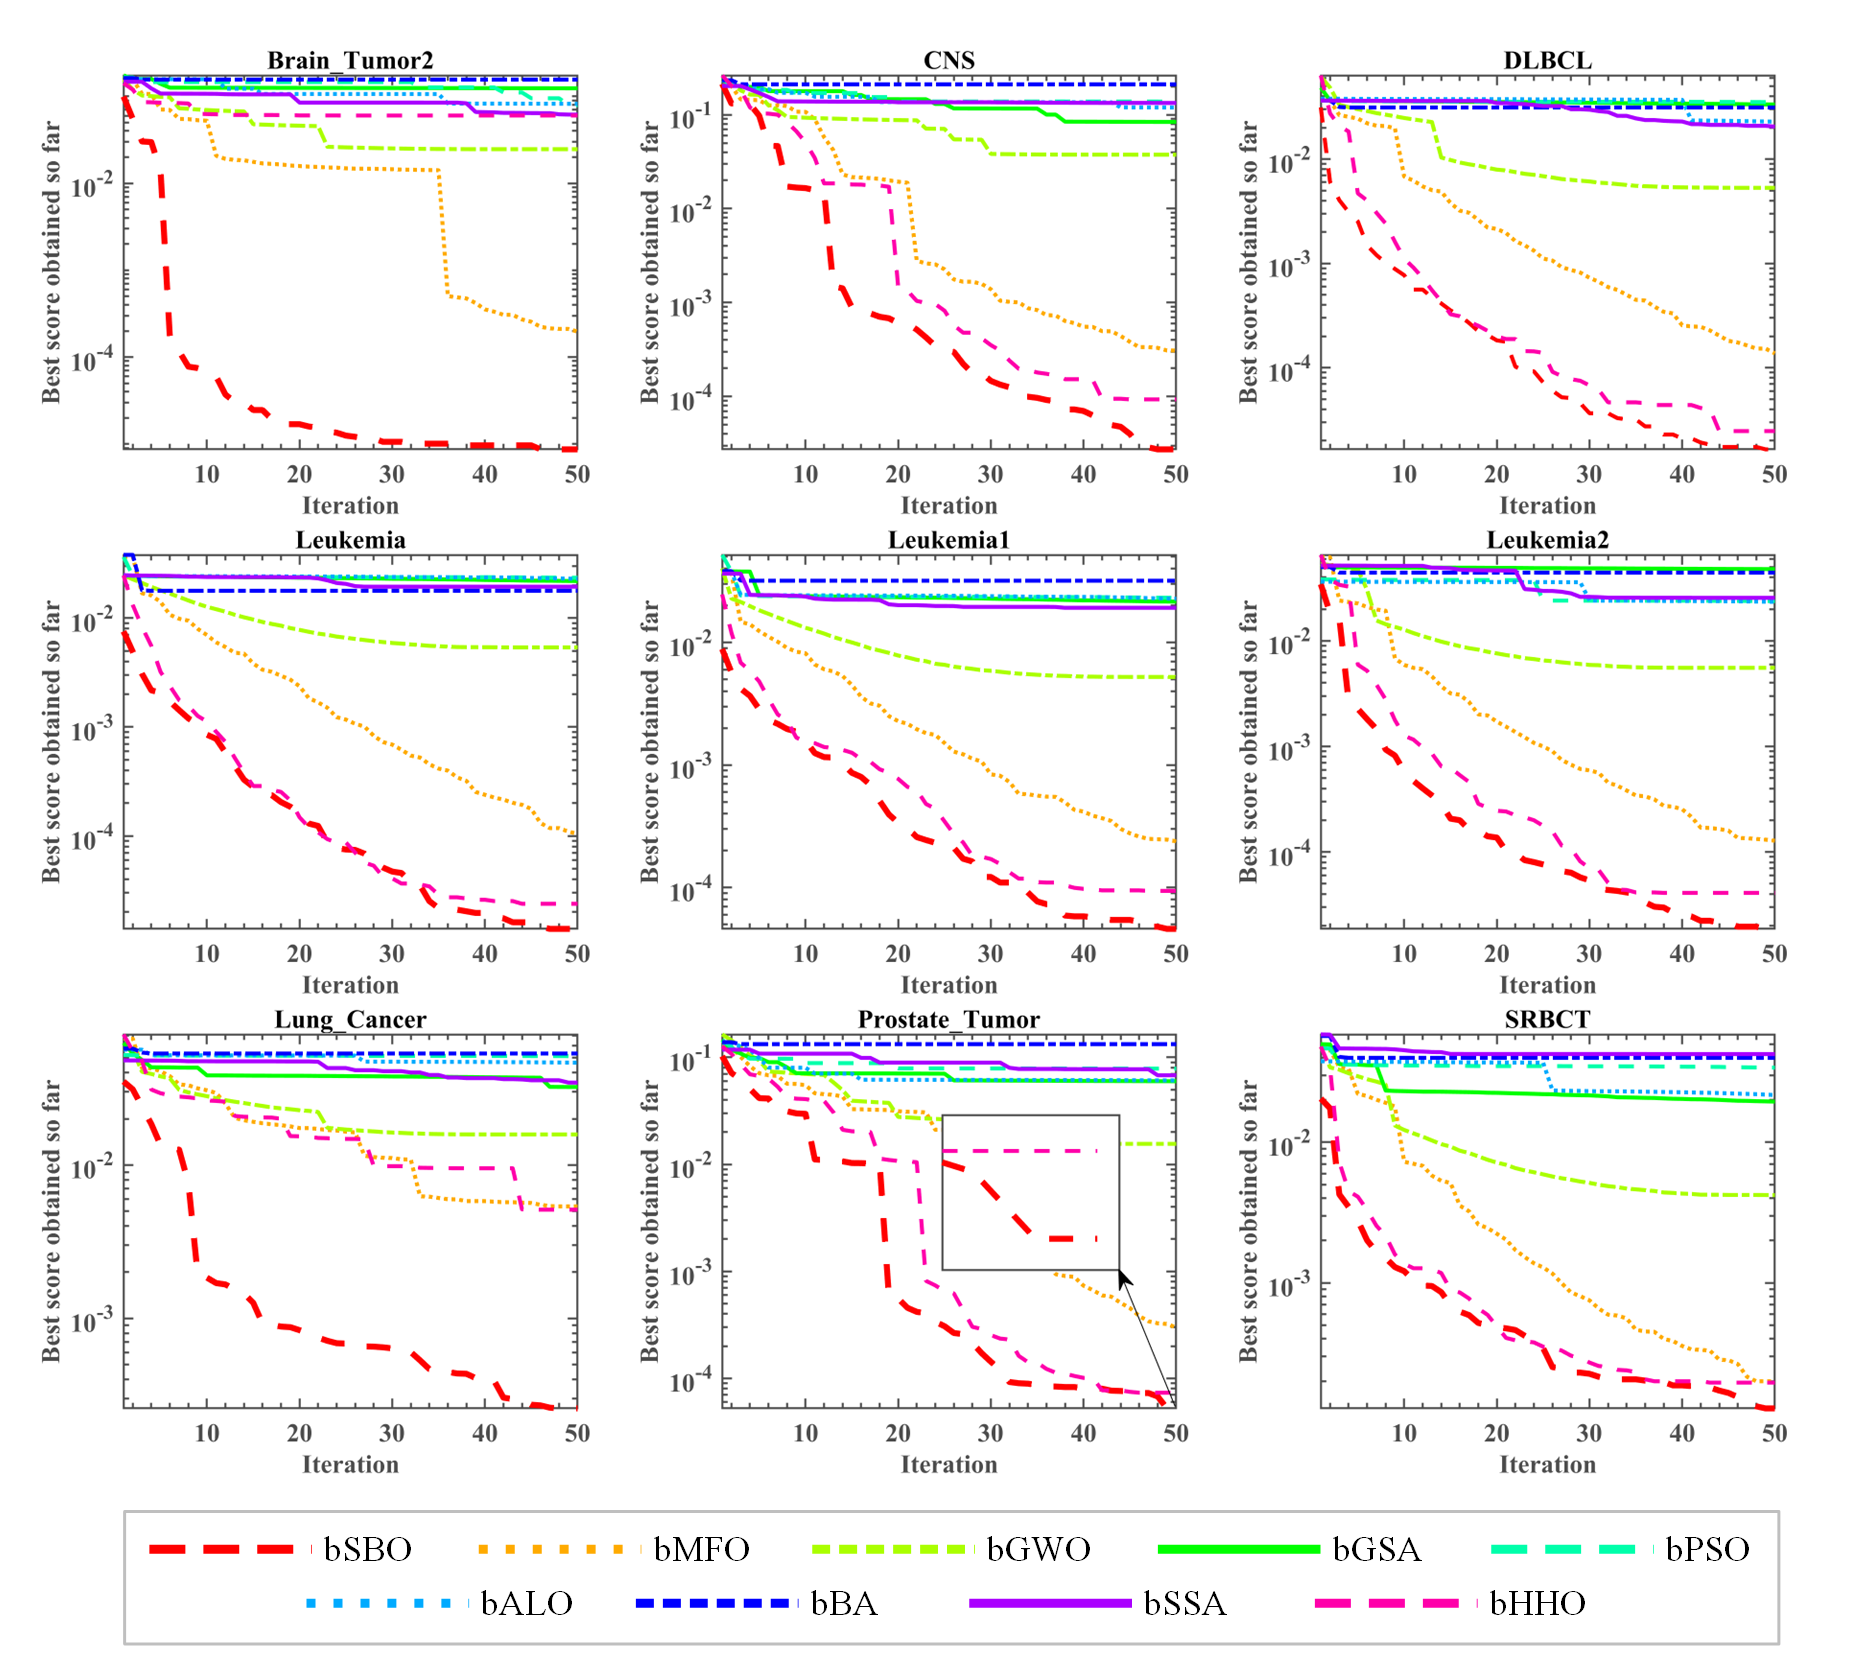
\includegraphics[width=\textwidth]{figures/fig14_convergence_bSBO.png}
  \caption{Convergence curves of bSBO and eight binary optimizers over nine datasets.}
  \label{fig:convergence_bSBO}
\end{figure}



The experimental results concerning the feature selection tasks effectively highlight the exceptional optimization capacity of bSBO, facilitated by the V-type transfer function, which adeptly translates the capabilities of the SBO algorithm from continuous to discrete optimization contexts. bSBO's performance has been comprehensively evaluated using three distinct metrics, underscoring its superior optimization abilities. These impressive results are attributed to the inherent global optimization strength of the SBO algorithm. Additionally, the mathematical modeling of human social upward mobility has granted SBO a distinct advantage, mirroring the way individuals connect and learn from high-status peers within complex social networks. By accessing and utilizing valuable information and resources, individuals can enhance their abilities---similar to how the SBO algorithm benefits from its comprehensive global search strategy, evolving toward improved solutions. This human-like learning and improvement dynamic within SBO is a testament to its design, significantly contributing to its effectiveness in feature selection tasks.

Building on this success, the following section extends the application of bSBO to the domain of image segmentation, where its optimization capabilities are leveraged to address multi-threshold segmentation challenges.


\paragraph{ Multi-threshold Image Segmentation}

Multi-threshold image segmentation is a critical process in image analysis that involves determining multiple optimal threshold values to partition an image into distinct regions based on intensity variations [79]. This technique not only facilitates the separation of key structures from the background but also enhances diagnostic accuracy in complex imaging scenarios, such as breast cancer detection. By delineating regions that represent various tissue types or pathological areas, multi-threshold segmentation plays a pivotal role in clinical decision-making and treatment planning.

Predominantly, multi-threshold segmentation methods can be classified into three categories: histogram-based, entropy-based, and optimization-based approaches---each characterized by unique threshold selection mechanisms. Histogram-based methods derive threshold candidates by analyzing the distribution of pixel intensities, thereby exploiting the natural clusters within the image data [80]. In contrast, entropy-based techniques, such as those using Kapur's or Tsallis entropy, aim to maximize the information content or homogeneity of the segmented regions [81]. Diverging from these, optimization-based methods cast the segmentation task as a search problem where a fitness function evaluates the quality of candidate threshold sets [82]. This latter approach often employs MAs, which are adept at navigating the high-dimensional search space and avoiding local optima, albeit at the cost of increased computational complexity.

This paper specifically focuses on searching for the optimal set of thresholds using Renyi entropy as the fitness function. By integrating Renyi entropy with a robust search strategy, our approach effectively addresses common challenges such as image noise and intensity inhomogeneity, thereby enhancing segmentation accuracy and computational efficiency. The subsequent sections detail the experimental settings, including the computing environment, parameter configurations, and performance evaluation metrics, followed by an application of our method to the segmentation of breast cancer images. Through these experiments, we demonstrate the potential of the proposed technique in accurately delineating tumor regions, ultimately contributing to improved diagnostic outcomes.


\subparagraph{ Experiment settings}

The performance of the proposed SBO for multi-threshold image segmentation was evaluated on a dataset comprising 9 breast cancer histology images. These images, sourced from the IDC dataset [83], were uniformly resized to 224 $\mathrm{\times}$ 224 pixels. Labeled sequentially from A to I, the images are shown in Fig. 15 along with their corresponding two-dimensional histograms, which illustrate the intensity distributions essential for threshold determination.

To assess the broad validity and robustness of the SBO method, segmentation experiments were conducted using three distinct threshold configurations---specifically, 6, 12, and 18 thresholds. The proposed SBO was compared against 7 advanced meta-heuristic algorithms, namely: Levy flight Slime Mould combined Opposition-based learning Improved Fruit fly Optimization Algorithm (LSEOFOA) [84], Improved Whale Optimization Algorithm (IWOA) [85], Improved Grey Wolf Optimizer (IGWO) [86], Adaptive Sin Cosine Algorithm (ASCA) [87], Iterative Mapping and Local Escaping Enhanced Salp Swarm Algorithm (ILSSA) [88], Effective Harris Hawks Algorithm Improved Salp Swarm Algorithm (EHSSA) [89], and Biogeography-Based Learning Particle Swarm Optimization (BLPSO) [90]. All methods were subjected to identical experimental conditions.

For each segmentation task, each algorithm was executed independently 30 times to mitigate the effects of stochastic variability. The mean (Avg) and standard deviation (Std) of the results were subsequently recorded. A uniform population size of 20 was maintained across all experiments, and each algorithm was terminated after 100 iterations to ensure fairness in comparative analysis. Moreover, all methods were run using the default parameter values as established in their original publications.

Segmentation quality was quantitatively evaluated using peak signal-to-noise ratio (PSNR), feature similarity index (FSIM), and structural similarity index (SSIM). These metrics collectively assess the fidelity, feature preservation, and structural integrity of the segmented images relative to the original data. The comprehensive experimental framework, with its controlled conditions and standardized evaluation criteria, provides a robust basis for comparing the performance of the SBO algorithm with other MA-based approaches.



\begin{figure}[htbp]
  \centering
  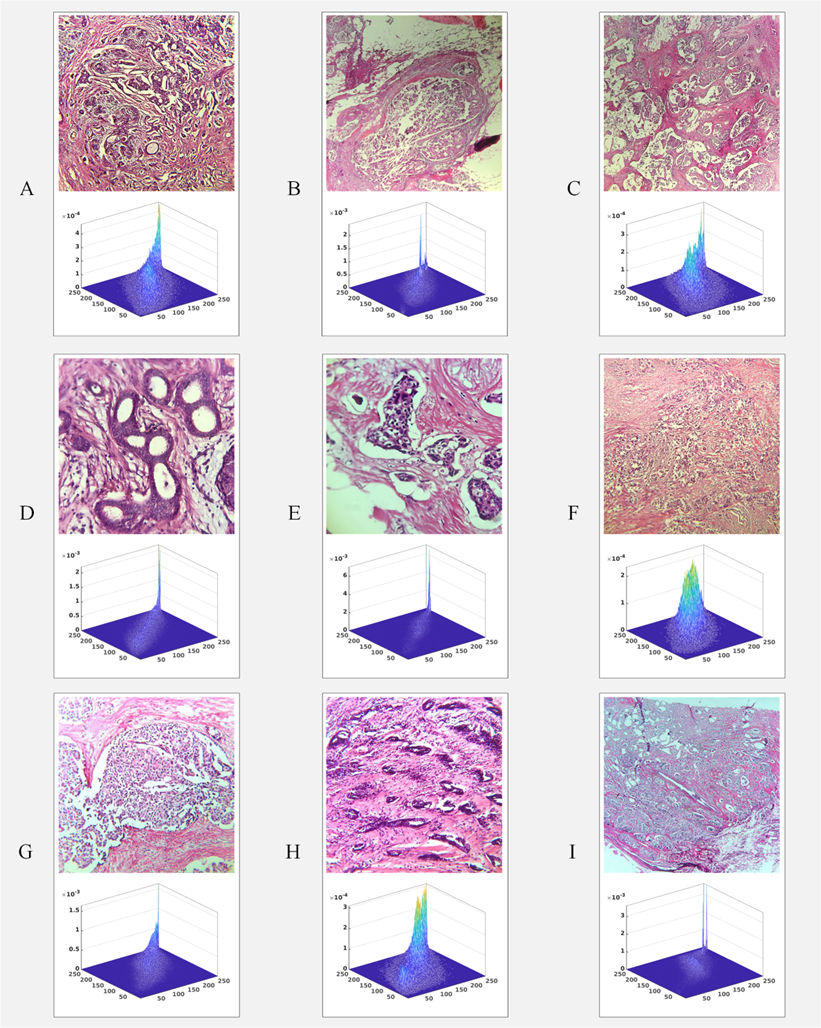
\includegraphics[width=\textwidth]{figures/fig15_original_images_2D_histogram.png}
  \caption{Original images and corresponding 2D-histogram.}
  \label{fig:original_images_2D_histogram}
\end{figure}




\subparagraph{ Experiment results and analysis}

The segmentation process for breast cancer images was implemented through a systematic and multi-stage pipeline, as illustrated in Fig. 16. The overall procedure is detailed as follows.

Initially, each breast cancer histology image is input and resized to a fixed dimension of 224 $\mathrm{\times}$ 224 pixels to ensure uniformity across the dataset. This standardization facilitates consistent processing and comparison of results. Subsequently, the resized images are converted into grayscale format, which simplifies the intensity analysis by reducing the image to a single channel while preserving essential structural information.

In parallel, a non-local means (NLM) filtering technique is applied to the grayscale images. This denoising step is critical for mitigating the effects of noise, thereby enhancing the quality of the image data for subsequent processing. The NLM algorithm exploits the redundancy in image patches to achieve effective noise reduction while preserving fine details.

The next phase involves the construction of a two-dimensional histogram, a pivotal component in our multi-threshold segmentation approach. This histogram is generated by combining the original grayscale image with its corresponding NLM-filtered version. The resulting NLM-based 2D histogram encapsulates both the intensity information and the texture features inherent in the image, providing a richer representation for threshold determination.

Following histogram construction, the threshold selection process is initiated. The MAs are employed to search for the optimal threshold values that maximize the chosen fitness function, specifically Renyi entropy. This optimization process systematically explores the solution space, identifying the threshold set those best partitions the image based on the combined intensity and texture cues.

Once the optimal threshold values have been determined, they are applied to segment the original image. This segmentation process divides the image into distinct regions corresponding to different intensity levels, effectively delineating areas of interest. The segmented image is then post-processed to generate a jet colormap representation, which visually enhances the delineation of boundaries and facilitates a more intuitive interpretation of the segmentation results.



\begin{figure}[htbp]
  \centering
  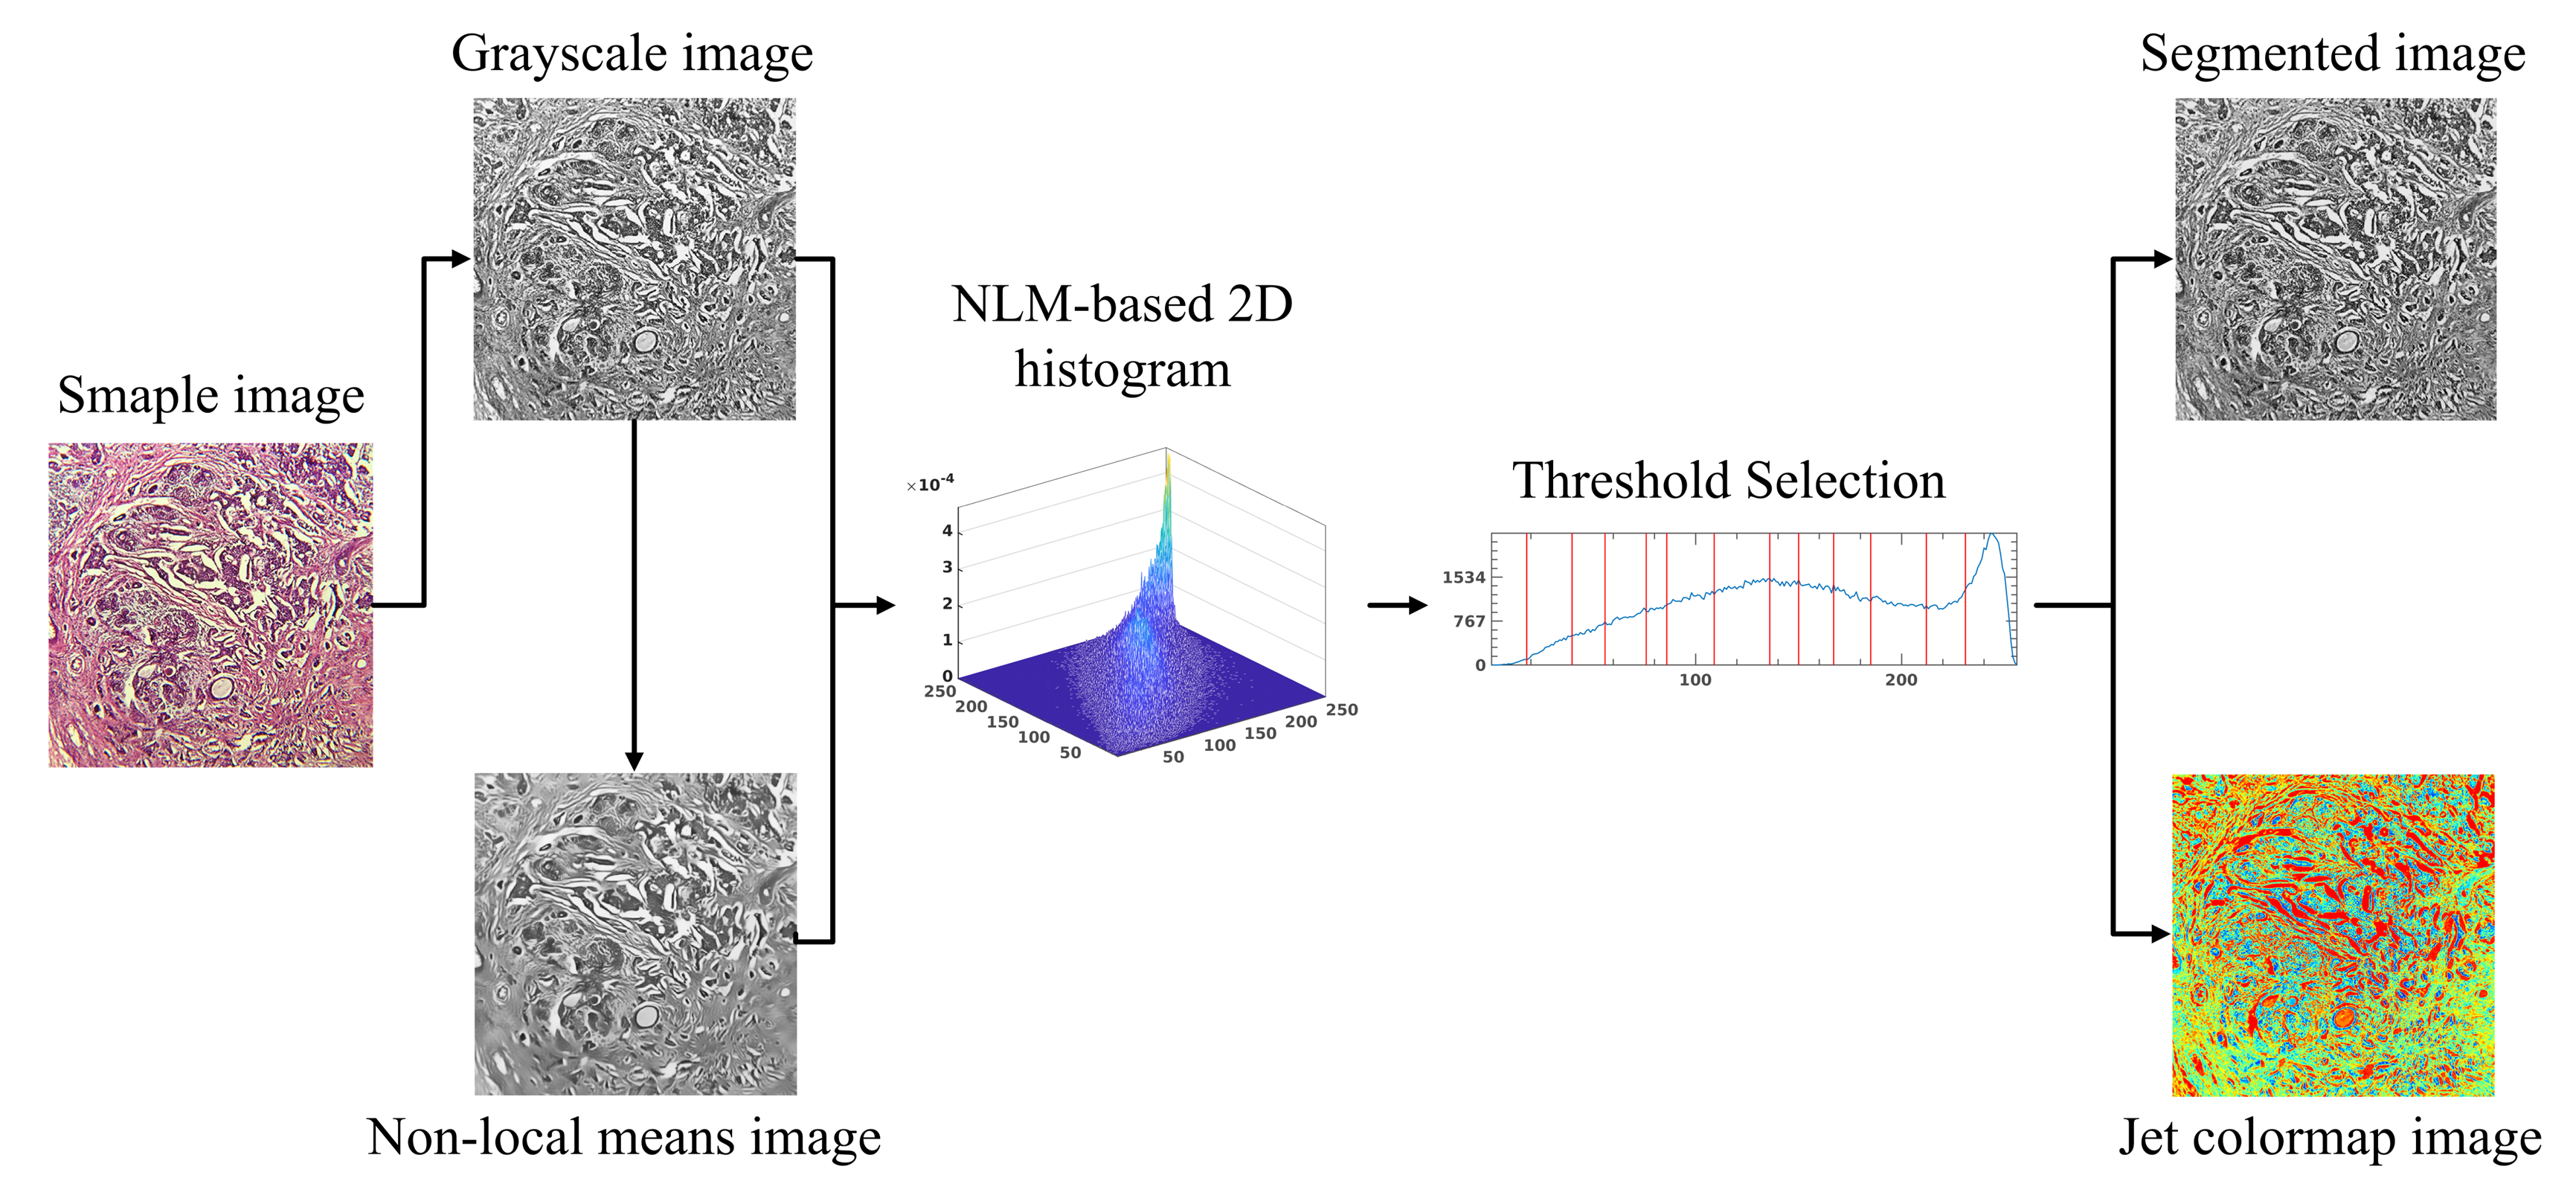
\includegraphics[width=\textwidth]{figures/fig16_flowchart_image_segmentation.png}
  \caption{Flowchart of multi-threshold image segmentation.}
  \label{fig:flowchart_image_segmentation}
\end{figure}



Following the segmentation pipeline detailed above, this section presents the experimental results, their analysis, and visualizations.

The performance of the proposed SBO-based model was evaluated using three widely adopted metrics: PSNR, FSIM, and SSIM. The results for segmentation tasks employing 6, 12, and 18 threshold levels are comprehensively summarized in Table A. 9\textbf{ through }Table A. 11, respectively. The metrics were computed for each threshold configuration over 30 independent runs, and the average and standard deviation values were reported. These tables highlight the optimal performance values in bold to facilitate straightforward recognition of the best results.

The performance metrics for the segmentation tasks using 6 thresholds are further visualized in Fig. 17, which presents a heatmap of the PSNR, FSIM, and SSIM scores. In this heatmap, warmer colors correspond to higher metric values, indicating superior segmentation quality, whereas cooler colors denote lower scores. A detailed analysis of these visualizations reveals that, across all three metrics, the proposed SBO-based approach consistently achieves the highest scores when compared with other evaluated methods.



\begin{figure}[htbp]
  \centering
  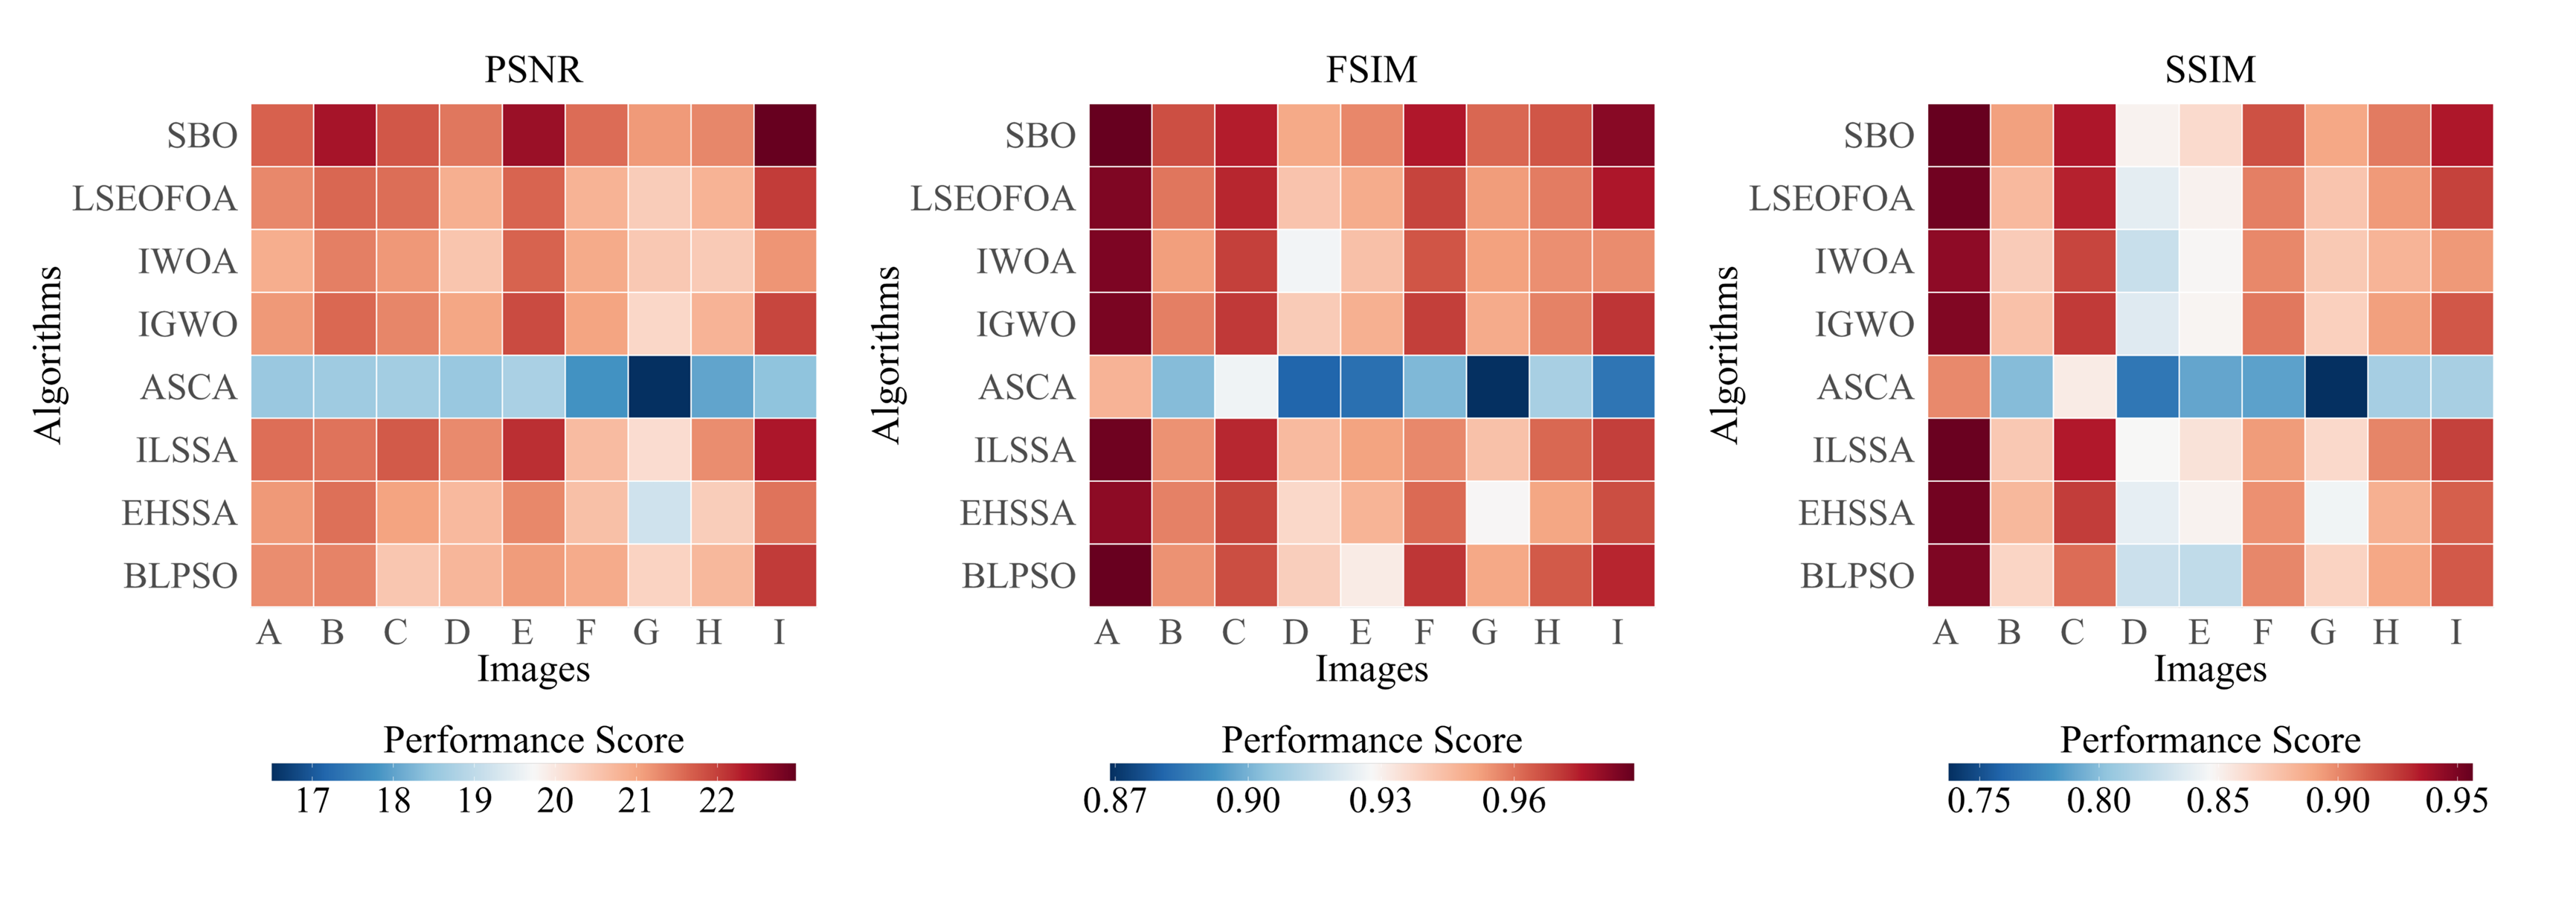
\includegraphics[width=\textwidth]{figures/fig17_heatmap_PSNR_FSIM_SSIM.png}
  \caption{Heatmap for PSNR, FSIM, and SSIM result over 6 threshold level.}
  \label{fig:heatmap_PSNR_FSIM_SSIM}
\end{figure}



In experiments conducted with 12 thresholds, Fig. 18 illustrates the convergence curve of the Renyi entropy value during the iterative optimization process. Although the SBO-based method initially exhibits lower entropy values during the early iterations, it steadily improves and ultimately converges to the optimal threshold configuration at the final iteration (iteration 100). This convergence behavior underscores the algorithm's capability to overcome initial suboptimality and effectively explore the solution space to identify the best threshold values.

\begin{figure}[htbp]
  \centering
  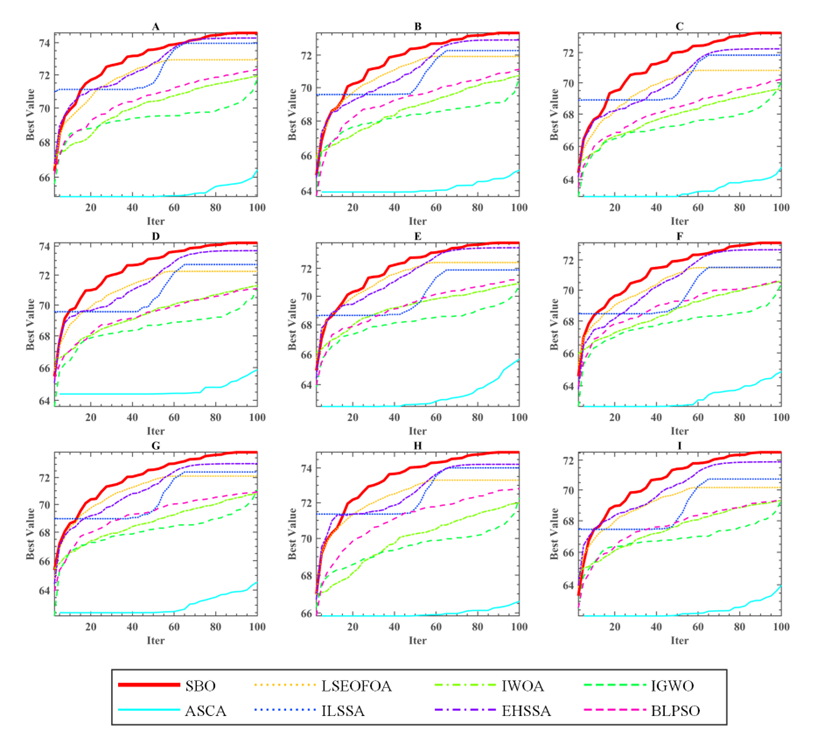
\includegraphics[width=\textwidth]{figures/fig18_convergence_entropy.png}
  \caption{Convergence curves of the entropy value by 12 threshold level.}
  \label{fig:convergence_entropy}
\end{figure}



For the segmentation tasks involving 18 thresholds, Fig. 19 compares the jet color mapped segmentation result for image B with its corresponding original image. The jet colormap enhances the visual interpretation by assigning distinct colors to regions of similar intensity. The comparative analysis demonstrates that the SBO-based method identifies more optimal thresholds, producing a segmented image where regions with analogous intensities are more accurately grouped together.

\begin{figure}[htbp]
  \centering
  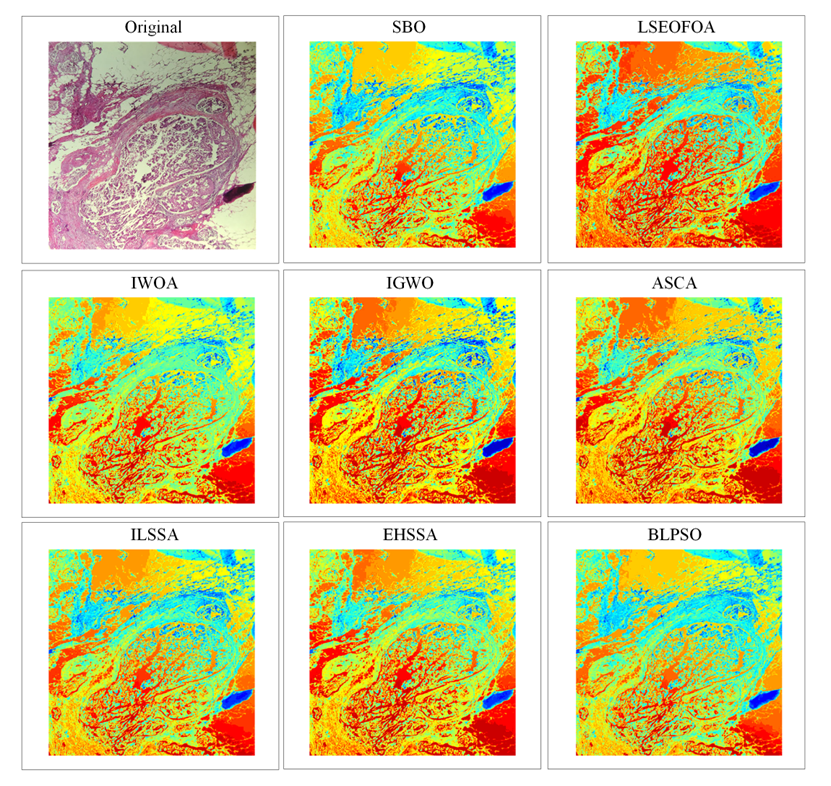
\includegraphics[width=\textwidth]{figures/fig19_jet_colormap_segmentation.png}
  \caption{Jet colormap segmentation result of image B over 18 threshold level.}
  \label{fig:jet_colormap_segmentation}
\end{figure}



Overall, the experimental results and accompanying visualizations provide compelling evidence of the superiority of the proposed SBO-based method. Across the various threshold levels and evaluation metrics, the approach yields higher quantitative scores and delivers visually coherent segmentation outcomes, thereby reinforcing its potential utility in clinical diagnostic applications.


\section{ Conclusions and Future Directions}

This paper introduces SBO, an MA inspired by human status-driven social behavior, where individuals seek advancement through strategic networking and resource exchange. SBO translates this dynamic into a computational model, balancing exploration and exploitation to navigate complex optimization landscapes efficiently. During exploration, agents move within a high-status circle defined by their own position, the most successful peer, and a high-status individual, ensuring diverse and effective searches. Exploitation is achieved through local refinements that enhance solution quality, ensuring convergence toward optimal solutions.

The SBO's effectiveness was validated across benchmark functions from the IEEE CEC 2017 suite, outperforming 13 state-of-the-art metaheuristics, including human-behavior-inspired algorithms, recent methods, and classical PSO and DE variants, across dimensions of 10, 30, 50, and 100. Statistical analyses, including the Wilcoxon signed-rank and Friedman tests, confirmed its superior global optimization capability and scalability. Further, a binary variant, bSBO, was developed for feature selection, leveraging a V-type transfer function to select minimal yet relevant feature subsets. Tested against 8 binary optimizers across 9 high-dimensional UCI datasets, bSBO consistently demonstrated optimal fitness, selecting the fewest features while maintaining high classification accuracy. SBO was also applied to multi-threshold image segmentation at 3 threshold levels, where it was compared with 7 advanced metaheuristic methods on 9 breast cancer histology images from the IDC dataset, effectively identifying optimal segmentation thresholds and highlighting its versatility in real-world applications.

Despite SBO's strong performance, in line with the No Free Lunch theorem [95], no algorithm excels in all scenarios. Future research should explore SBO's adaptation to multi-objective optimization, scalability for large-scale problems, and hybridization with other computational frameworks to enhance its robustness and applicability. Further testing across diverse domains will provide deeper insights into its optimization potential and contribute to advancing heuristic optimization methodologies.

Moreover, recent advances in dynamic multi-objective optimization, such as the non-inductive transfer learning approach with multi-strategy adaptive selection [91] and the cascaded fuzzy system for objective knowledge transfer [92], offer valuable insights for further enhancement. These approaches address challenges like negative transfer and rigid labeling in dynamic environments and may inspire future extensions of SBO to handle time-varying optimization problems effectively. In our future work, we plan to investigate the integration of such advanced techniques into SBO, aiming to further improve its adaptability and performance in dynamic settings.

\noindent 
\section{Acknowledgments}

This work was supported by the``Pioneering Leadership + X'' Research and Development Plan of Zhejiang Provincial Department of Science and Technology (2024C03237) and the Natural Science Foundation of Hangzhou (2024SZRYBH180010), Zhejiang Provincial Natural Science Foundation of China under Grant No. LR23F020001, and Major Science and Technology Plan Projects in Zhejiang Province under Grant No. 2025C01074.

\noindent \textbf{Data Availability declaration}

\noindent The datasets generated during and analyzed during the current study are available from the corresponding author on reasonable request.

\noindent \textbf{Competing Interests}

\noindent The authors declare that they have no conflicts of interests or competing interests.\textbf{}

\noindent \textbf{Compliance with Ethical Standards}

\noindent Ethical approval: This article does not contain any studies with human participants performed by any of the authors.

\noindent 

\noindent \textbf{Declaration of AI and AI-assisted technologies in the writing process}

\noindent During the preparation of this work, the author(s) used ChatGPT to improve and proofread the English of the paper. After using this tool/service, the author(s) reviewed and edited the content as needed and take(s) full responsibility for the content of the publication.

\noindent 

\noindent \textbf{CRediT author statement}

\noindent \textbf{Jian Wang:}~Conceptualization, Methodology, Software, Validation, Formal Analysis, Visualization, Investigation, Data Curation, Writing - Original Draft\textbf{Yi Chen:}~Methodology, Software, Validation, Visualization, Writing - Original Draft, Writing - Review \& Editing, Supervision\textbf{Chenglang Lu:}~Formal Analysis, Investigation, Resources, Data Curation, Writing - Original Draft, Project Administration, Funding Acquisition\textbf{Ali Asghar Heidari:}~ Software, Validation, Formal Analysis, Writing - Review \& Editing, Supervision, Writing - Original Draft\textbf{Zongda Wu:}~Investigation, Visualization, Writing - Original Draft, Writing - Review \& Editing, Resources, Funding Acquisition\textbf{Huiling Chen:}~ Validation, Formal Analysis, Writing - Original Draft, Writing - Review \& Editing, Supervision

\noindent 

\noindent 
\section{Appendix}

 See Table A. 1-A. 11.

\begin{tabular}{|p{0.3in}|p{0.3in}|p{0.3in}|p{0.3in}|p{0.3in}|p{0.3in}|p{0.3in}|p{0.3in}|p{0.3in}|p{0.3in}|p{0.3in}|p{0.3in}|p{0.3in}|p{0.3in}|p{0.3in}|p{0.5in}|} \hline 
\multicolumn{16}{|p{4.8in}|}{\textbf{Table A. }1\textbf{. }Comparative results of SBO and state-of-the-art algorithms for 10-dimensional problems.\textbf{}} \\ \hline 
Fun & Item & SBO & TLBO & PO & HHO & RIME & ALCPSO & CLPSO & CGPSO & MSPSO & CMAES & DECLS & LSHADE\_cnEpSin & SCADE & SHADE \\ \hline 
F1 & Avg & 1.0000E+02 & 2.3180E+09 & 5.7825E+07 & 2.7350E+05 & 1.1951E+03 & 8.5399E+02 & 1.0876E+02 & 5.4781E+06 & 4.7180E+02 & \textbf{1.0000E+02} & 4.4133E+02 & \textbf{1.0000E+02} & 9.4471E+08 & \textbf{1.0000E+02} \\ \hline 
 & Std & 3.7899E-11 & 1.9307E+09 & 1.7239E+08 & 1.2752E+05 & 8.7649E+02 & 6.8933E+02 & 1.2166E+01 & 1.4214E+06 & 4.8450E+02 & \textbf{0.0000E+00} & 3.6559E+02 & 2.0441E-14 & 3.7498E+08 & \textbf{0.0000E+00} \\ \hline 
F2 & Avg & \textbf{3.0000E+02} & 5.6759E+03 & 3.0009E+02 & 3.0148E+02 & 3.0000E+02 & 3.6480E+02 & 3.0284E+02 & 3.2021E+02 & 3.0000E+02 & \textbf{3.0000E+02} & 9.5474E+02 & \textbf{3.0000E+02} & 3.4003E+03 & \textbf{3.0000E+02} \\ \hline 
 & Std & 4.4783E-14 & 3.5880E+03 & 4.5599E-01 & 8.6163E-01 & 2.7309E-03 & 2.1593E+02 & 2.1596E+00 & 6.3013E+00 & 4.4408E-08 & \textbf{0.0000E+00} & 4.1849E+02 & 3.5009E-14 & 1.1183E+03 & \textbf{0.0000E+00} \\ \hline 
F3 & Avg & 4.1681E+02 & 6.8320E+02 & 4.3204E+02 & 4.2885E+02 & 4.2373E+02 & 4.1831E+02 & 4.0063E+02 & 4.0779E+02 & \textbf{4.0000E+02} & 4.3130E+02 & 4.1887E+02 & 4.2302E+02 & 4.8082E+02 & 4.2927E+02 \\ \hline 
 & Std & 1.7155E+01 & 3.9742E+02 & 2.4709E+01 & 1.6903E+01 & 2.0094E+01 & 1.8927E+01 & 7.2505E-01 & 2.1031E+00 & \textbf{4.0814E-12} & 1.0612E+01 & 1.2199E+01 & 1.2929E+01 & 1.5995E+01 & 1.2557E+01 \\ \hline 
F4 & Avg & 5.2103E+02 & 5.3686E+02 & 5.4090E+02 & 5.3752E+02 & 5.1081E+02 & 5.1535E+02 & 5.0523E+02 & 5.3135E+02 & 5.2759E+02 & 6.9599E+02 & 5.0828E+02 & \textbf{5.0408E+02} & 5.4742E+02 & 5.0484E+02 \\ \hline 
 & Std & 1.0955E+01 & 1.2216E+01 & 2.2018E+01 & 1.5707E+01 & 3.7660E+00 & 7.0510E+00 & \textbf{1.3200E+00} & 1.3347E+01 & 8.2334E+00 & 1.1764E+02 & 1.4219E+00 & 1.8906E+00 & 6.1203E+00 & 1.8427E+00 \\ \hline 
F5 & Avg & 6.0000E+02 & 6.2154E+02 & 6.0194E+02 & 6.3246E+02 & 6.0002E+02 & 6.0000E+02 & \textbf{6.0000E+02} & 6.0495E+02 & 6.0932E+02 & 6.8167E+02 & \textbf{6.0000E+02} & 6.0000E+02 & 6.1657E+02 & 6.0000E+02 \\ \hline 
 & Std & 4.8843E-03 & 6.4558E+00 & 7.1750E+00 & 7.7477E+00 & 7.9383E-03 & 5.4205E-03 & 6.6759E-14 & 4.6937E+00 & 1.0207E+01 & 1.8514E+01 & \textbf{3.6566E-14} & 2.8894E-04 & 3.2689E+00 & 1.8204E-05 \\ \hline 
F6 & Avg & 7.2736E+02 & 7.9128E+02 & 7.2114E+02 & 8.0159E+02 & 7.2062E+02 & 7.2288E+02 & 7.1630E+02 & 7.3992E+02 & 7.2248E+02 & 1.5829E+03 & 7.1971E+02 & \textbf{7.1338E+02} & 7.8912E+02 & 7.1427E+02 \\ \hline 
 & Std & 7.2747E+00 & 3.5415E+01 & 6.5920E+00 & 3.1667E+01 & 4.9622E+00 & 4.9199E+00 & \textbf{1.3102E+00} & 6.1315E+00 & 5.0845E+00 & 4.1952E+02 & 2.1805E+00 & 1.5493E+00 & 1.3146E+01 & 2.3054E+00 \\ \hline 
F7 & Avg & 8.2225E+02 & 8.3788E+02 & 8.2739E+02 & 8.4522E+02 & 8.1232E+02 & 8.1242E+02 & 8.0513E+02 & 8.3708E+02 & 8.2987E+02 & 9.8467E+02 & 8.0861E+02 & \textbf{8.0441E+02} & 8.5401E+02 & 8.0444E+02 \\ \hline 
 & Std & 9.2619E+00 & 1.1309E+01 & 1.5845E+01 & 1.3262E+01 & 4.6139E+00 & 4.5775E+00 & \textbf{1.1352E+00} & 1.0167E+01 & 8.3229E+00 & 7.1960E+01 & 1.7763E+00 & 1.5596E+00 & 9.0722E+00 & 1.3255E+00 \\ \hline 
F8 & Avg & 9.0158E+02 & 1.1883E+03 & 1.8315E+03 & 1.7995E+03 & 9.0004E+02 & 9.0045E+02 & 9.0000E+02 & 9.5939E+02 & 1.1690E+03 & 4.7794E+03 & \textbf{9.0000E+02} & 9.0013E+02 & 1.1973E+03 & 9.0007E+02 \\ \hline 
 & Std & 3.0779E+00 & 1.8033E+02 & 1.4153E+02 & 2.9037E+02 & 1.1647E-01 & 6.6575E-01 & 4.3803E-07 & 1.8652E+02 & 2.5310E+02 & 1.3525E+03 & \textbf{0.0000E+00} & 2.7253E-01 & 1.3439E+02 & 1.5588E-01 \\ \hline 
F9 & Avg & 1.3851E+03 & 1.9715E+03 & 1.6257E+03 & 1.8197E+03 & 1.2828E+03 & 1.4065E+03 & 1.1400E+03 & 1.9250E+03 & 1.5005E+03 & 2.6178E+03 & 1.3735E+03 & \textbf{1.0878E+03} & 2.3300E+03 & 1.1061E+03 \\ \hline 
 & Std & 2.6189E+02 & 2.6708E+02 & 1.8066E+02 & 3.0548E+02 & 1.9557E+02 & 2.8974E+02 & \textbf{6.3268E+01} & 2.2613E+02 & 1.6301E+02 & 4.6360E+02 & 1.2582E+02 & 7.2997E+01 & 1.5129E+02 & 8.9242E+01 \\ \hline 
F10 & Avg & 1.1083E+03 & 1.1963E+03 & 1.8307E+03 & 1.1314E+03 & 1.1079E+03 & 1.1123E+03 & 1.1025E+03 & 1.1175E+03 & 1.1127E+03 & 1.1263E+03 & 1.1032E+03 & 1.1071E+03 & 1.2089E+03 & \textbf{1.1018E+03} \\ \hline 
 & Std & 4.2547E+00 & 9.5005E+01 & 2.9738E+03 & 2.0663E+01 & 4.2869E+00 & 1.2376E+01 & 1.0394E+00 & 7.7493E+00 & 7.3783E+00 & 1.5009E+01 & \textbf{1.0077E+00} & 8.0343E+00 & 3.7841E+01 & 1.2827E+00 \\ \hline 
F11 & Avg & 2.0189E+03 & 1.1538E+06 & 4.0045E+05 & 4.1113E+06 & 1.8147E+04 & 2.1672E+04 & 1.8209E+04 & 1.2964E+06 & 2.6195E+03 & 1.6768E+03 & 7.1923E+04 & 1.6599E+03 & 1.4365E+07 & \textbf{1.4866E+03} \\ \hline 
 & Std & 1.2392E+03 & 2.2445E+06 & 9.0075E+05 & 5.2074E+06 & 1.3042E+04 & 1.3461E+04 & 1.7372E+04 & 1.5018E+06 & 2.8892E+03 & 1.9643E+02 & 4.2183E+04 & 2.3576E+02 & 9.1844E+06 & \textbf{1.6495E+02} \\ \hline 
F12 & Avg & 1.3090E+03 & 2.9516E+03 & 1.4632E+04 & 1.7880E+04 & 3.5650E+03 & 3.9140E+03 & 1.3348E+03 & 9.5724E+03 & 1.3683E+03 & 1.4794E+03 & 2.1266E+03 & 1.3679E+03 & 2.9126E+04 & \textbf{1.3048E+03} \\ \hline 
 & Std & 4.9077E+00 & 2.3298E+03 & 1.2823E+04 & 2.1559E+04 & 2.5377E+03 & 2.0317E+03 & 2.7892E+01 & 6.1609E+03 & 4.4587E+01 & 1.0798E+02 & 1.1207E+03 & 1.0372E+02 & 2.0590E+04 & \textbf{2.2110E+00} \\ \hline 
F13 & Avg & 1.4263E+03 & 1.4850E+03 & 3.1339E+03 & 1.7509E+03 & 1.4372E+03 & 1.5841E+03 & 1.4543E+03 & 1.4650E+03 & 1.4590E+03 & 1.5504E+03 & 1.5103E+03 & 1.4245E+03 & 1.5449E+03 & \textbf{1.4078E+03} \\ \hline 
 & Std & \textbf{5.4817E+00} & 4.0451E+01 & 5.8398E+02 & 4.2267E+02 & 5.3315E+01 & 6.9207E+02 & 4.4814E+01 & 2.2583E+01 & 1.6827E+01 & 1.5352E+02 & 1.1610E+02 & 1.3122E+01 & 5.6534E+01 & 8.7392E+00 \\ \hline 
F14 & Avg & 1.5073E+03 & 1.5637E+03 & 1.9624E+03 & 1.8549E+03 & 1.5225E+03 & 1.5894E+03 & 1.5453E+03 & 1.6129E+03 & 1.5224E+03 & 1.5537E+03 & 1.5728E+03 & 1.5103E+03 & 1.6910E+03 & \textbf{1.5010E+03} \\ \hline 
 & Std & 8.6049E+00 & 3.1139E+01 & 2.0039E+02 & 1.9634E+02 & 1.8791E+01 & 8.5496E+01 & 8.5575E+01 & 5.9174E+01 & 1.0945E+01 & 4.2251E+01 & 4.5576E+01 & 1.3395E+01 & 5.2441E+01 & \textbf{1.3910E+00} \\ \hline 
F15 & Avg & 1.6771E+03 & 1.7305E+03 & 1.9410E+03 & 1.7459E+03 & 1.6753E+03 & 1.6918E+03 & \textbf{1.6039E+03} & 1.7392E+03 & 1.6859E+03 & 1.9583E+03 & 1.6136E+03 & 1.6195E+03 & 1.6828E+03 & 1.6066E+03 \\ \hline 
 & Std & 6.5089E+01 & 7.4316E+01 & 1.7173E+02 & 6.2056E+01 & 7.2370E+01 & 6.4484E+01 & \textbf{3.4275E+00} & 7.3715E+01 & 5.6257E+01 & 2.2731E+02 & 8.8343E+00 & 4.0494E+01 & 6.3896E+01 & 2.1877E+01 \\ \hline 
F16 & Avg & 1.7380E+03 & 1.7482E+03 & 1.7381E+03 & 1.7500E+03 & 1.7478E+03 & 1.7548E+03 & 1.7288E+03 & 1.7492E+03 & 1.7354E+03 & 1.8871E+03 & 1.7328E+03 & \textbf{1.7248E+03} & 1.7755E+03 & 1.7250E+03 \\ \hline 
 & Std & 9.2807E+00 & 1.5395E+01 & \textbf{3.5389E+00} & 1.5522E+01 & 3.6749E+01 & 3.3858E+01 & 4.8536E+00 & 9.6468E+00 & 6.2288E+00 & 1.9391E+02 & 4.4028E+00 & 6.8232E+00 & 9.9580E+00 & 3.5507E+00 \\ \hline 
F17 & Avg & 1.8636E+03 & 2.5766E+03 & 7.8245E+03 & 1.4442E+04 & 6.3295E+03 & 8.5061E+03 & 2.4236E+03 & 1.1574E+04 & 1.8681E+03 & 1.8538E+03 & 4.2864E+03 & 1.8412E+03 & 2.0925E+04 & \textbf{1.8250E+03} \\ \hline 
 & Std & 4.9864E+01 & 1.1615E+03 & 5.3044E+03 & 7.0133E+03 & 4.4974E+03 & 7.2177E+03 & 6.0648E+02 & 6.4248E+03 & 2.3702E+01 & 2.1465E+01 & 2.0536E+03 & \textbf{1.5729E+01} & 1.0980E+04 & 1.7644E+01 \\ \hline 
F18 & Avg & 1.9027E+03 & 1.9639E+03 & 4.3548E+03 & 3.0481E+03 & 1.9050E+03 & 1.9636E+03 & 1.9137E+03 & 1.9981E+03 & 1.9144E+03 & 1.9615E+03 & 1.9274E+03 & 1.9078E+03 & 2.4347E+03 & \textbf{1.9010E+03} \\ \hline 
 & Std & 1.9354E+00 & 5.5729E+01 & 3.4496E+03 & 1.7149E+03 & 2.4059E+00 & 1.2416E+02 & 1.9147E+01 & 1.0295E+02 & 7.3152E+00 & 3.9553E+01 & 9.4558E+01 & 1.6371E+01 & 4.5388E+02 & \textbf{1.0705E+00} \\ \hline 
F19 & Avg & 2.0167E+03 & 2.0785E+03 & 2.0964E+03 & 2.1739E+03 & 2.0225E+03 & 2.0340E+03 & 2.0090E+03 & 2.1462E+03 & 2.1310E+03 & 2.6039E+03 & 2.0110E+03 & 2.0134E+03 & 2.1197E+03 & \textbf{2.0079E+03} \\ \hline 
 & Std & 1.5761E+01 & 3.2707E+01 & 5.4794E+01 & 6.0679E+01 & 1.1842E+01 & 2.3483E+01 & 8.1163E+00 & 6.0332E+01 & 4.6628E+01 & 2.0009E+02 & 6.7090E+00 & 1.0955E+01 & 2.4363E+01 & \textbf{5.4583E+00} \\ \hline 
F20 & Avg & \textbf{2.2800E+03} & 2.2854E+03 & 2.2801E+03 & 2.2811E+03 & 2.2801E+03 & \textbf{2.2800E+03} & \textbf{2.2800E+03} & 2.2874E+03 & 2.2800E+03 & \textbf{2.2800E+03} & \textbf{2.2800E+03} & \textbf{2.2800E+03} & 2.2804E+03 & \textbf{2.2800E+03} \\ \hline 
 & Std & 4.0684E+01 & 2.9706E+01 & 4.0429E+01 & 3.8365E+01 & 4.0439E+01 & 4.0684E+01 & 4.0684E+01 & \textbf{2.5672E+01} & 4.0684E+01 & 4.0684E+01 & 4.0684E+01 & 4.0684E+01 & 3.9871E+01 & 4.0684E+01 \\ \hline 
F21 & Avg & 2.2327E+03 & 2.2829E+03 & 2.2904E+03 & 2.2465E+03 & 2.2270E+03 & 2.2316E+03 & \textbf{2.2175E+03} & 2.2555E+03 & 2.2420E+03 & 2.3083E+03 & 2.2223E+03 & 2.2219E+03 & 2.2797E+03 & 2.2216E+03 \\ \hline 
 & Std & 3.4761E+01 & 3.9109E+01 & 2.6473E+01 & 3.2342E+01 & 3.7815E+01 & 3.5065E+01 & 3.7684E+01 & 4.0256E+01 & 3.0143E+01 & 8.1809E+01 & 3.9657E+01 & 3.9879E+01 & \textbf{1.5061E+01} & 3.9970E+01 \\ \hline 
F22 & Avg & \textbf{2.5000E+03} & \textbf{2.5000E+03} & 2.5260E+03 & \textbf{2.5000E+03} & 2.6665E+03 & 2.6629E+03 & 2.6443E+03 & 2.5160E+03 & 2.6571E+03 & 3.7417E+03 & 2.5469E+03 & 2.6501E+03 & 2.5071E+03 & 2.6520E+03 \\ \hline 
 & Std & \textbf{0.0000E+00} & 8.4444E-14 & 6.7607E+01 & \textbf{0.0000E+00} & 9.6352E+00 & 5.0656E+01 & 2.8120E+01 & 8.7666E+01 & 1.1120E+02 & 3.6362E+02 & 7.2968E+01 & 4.4361E+00 & 3.8827E+01 & 6.8170E+00 \\ \hline 
F23 & Avg & 2.6000E+03 & 2.6000E+03 & 2.6000E+03 & 2.6000E+03 & 2.7597E+03 & 2.7265E+03 & \textbf{2.5176E+03} & 2.6000E+03 & 2.5967E+03 & 2.6662E+03 & 2.5969E+03 & 2.7289E+03 & 2.6000E+03 & 2.7672E+03 \\ \hline 
 & Std & \textbf{0.0000E+00} & 2.8007E-13 & \textbf{0.0000E+00} & \textbf{0.0000E+00} & 9.2116E+01 & 1.1652E+02 & 2.3710E+01 & 2.6163E-02 & 1.8257E+01 & 1.0591E+02 & 1.6742E+01 & 1.0063E+02 & \textbf{0.0000E+00} & 8.7201E+01 \\ \hline 
F24 & Avg & \textbf{2.7000E+03} & \textbf{2.7000E+03} & \textbf{2.7000E+03} & \textbf{2.7000E+03} & 2.9361E+03 & 2.9322E+03 & 2.8662E+03 & 2.7001E+03 & 2.9312E+03 & 2.9360E+03 & 2.7000E+03 & 2.9260E+03 & \textbf{2.7000E+03} & 2.9248E+03 \\ \hline 
 & Std & \textbf{0.0000E+00} & 2.6704E-13 & \textbf{0.0000E+00} & \textbf{0.0000E+00} & 2.5218E+01 & 2.2256E+01 & 6.8001E+01 & 2.8371E-01 & 4.7188E+01 & 1.8573E+01 & 1.0346E-02 & 2.2547E+01 & \textbf{0.0000E+00} & 2.3799E+01 \\ \hline 
F25 & Avg & 2.8000E+03 & 2.8000E+03 & 2.8000E+03 & 2.8000E+03 & 3.0581E+03 & 3.1611E+03 & 2.7796E+03 & 2.8000E+03 & 2.8000E+03 & 3.4923E+03 & \textbf{2.7788E+03} & 2.9453E+03 & 2.8000E+03 & 3.0323E+03 \\ \hline 
 & Std & \textbf{0.0000E+00} & 3.8697E-13 & \textbf{0.0000E+00} & \textbf{0.0000E+00} & 2.4113E+02 & 2.6157E+02 & 8.8635E+01 & 6.2322E-03 & 6.1154E-05 & 9.4207E+02 & 4.7037E+01 & 1.6037E+02 & \textbf{0.0000E+00} & 2.2056E+02 \\ \hline 
F26 & Avg & \textbf{2.9000E+03} & 2.9109E+03 & 2.9324E+03 & \textbf{2.9000E+03} & 3.1469E+03 & 3.2161E+03 & 3.1336E+03 & 2.9702E+03 & 3.3521E+03 & 4.2311E+03 & 2.9549E+03 & 3.1660E+03 & 2.9869E+03 & 3.1491E+03 \\ \hline 
 & Std & \textbf{0.0000E+00} & 5.9926E+01 & 1.0060E+02 & \textbf{0.0000E+00} & 3.8290E+01 & 7.2678E+01 & 1.2388E+01 & 2.0495E+02 & 1.2320E+02 & 1.2932E+03 & 1.0127E+02 & 5.5653E+01 & 1.2825E+02 & 3.3855E+01 \\ \hline 
F27 & Avg & \textbf{3.0000E+03} & \textbf{3.0000E+03} & 3.0476E+03 & \textbf{3.0000E+03} & 3.1340E+03 & 3.1336E+03 & 3.1008E+03 & 3.0001E+03 & 3.1292E+03 & 3.1469E+03 & 3.0000E+03 & 3.1294E+03 & \textbf{3.0000E+03} & 3.1307E+03 \\ \hline 
 & Std & \textbf{0.0000E+00} & 2.2342E-13 & 1.4572E+02 & \textbf{0.0000E+00} & 2.5453E+01 & 2.7844E+01 & 3.0353E+01 & 1.7858E-01 & 4.0294E+01 & 3.4520E+01 & 9.4064E-03 & 2.4392E+01 & \textbf{0.0000E+00} & 2.6477E+01 \\ \hline 
F28 & Avg & 3.1027E+03 & 3.1040E+03 & 3.1432E+03 & \textbf{3.1000E+03} & 3.1736E+03 & 3.1862E+03 & 3.1548E+03 & 3.1693E+03 & 3.1614E+03 & 3.3139E+03 & 3.1515E+03 & 3.1444E+03 & 3.2006E+03 & 3.1509E+03 \\ \hline 
 & Std & 9.9386E+00 & 2.0706E+01 & 5.6733E+01 & \textbf{0.0000E+00} & 3.6379E+01 & 3.3949E+01 & 2.0757E+01 & 5.2902E+01 & 1.9386E+01 & 1.6788E+02 & 3.0011E+01 & 8.4873E+00 & 1.7336E+01 & 9.0005E+00 \\ \hline 
F29 & Avg & 3.2575E+03 & 4.7588E+03 & \textbf{3.2000E+03} & 6.1051E+03 & 1.2111E+04 & 1.1138E+04 & 5.5652E+03 & 7.6245E+03 & 3.7131E+03 & 3.3027E+03 & 9.1510E+03 & 3.3174E+03 & 4.2189E+04 & 3.2729E+03 \\ \hline 
 & Std & 1.3251E+02 & 2.9276E+03 & \textbf{0.0000E+00} & 1.1146E+04 & 9.2233E+03 & 6.3386E+03 & 1.6372E+03 & 7.4466E+03 & 2.3594E+02 & 7.6152E+01 & 7.3674E+03 & 6.4934E+01 & 6.6794E+04 & 5.1380E+01 \\ \hline 
\end{tabular}



\begin{tabular}{|p{0.3in}|p{0.3in}|p{0.3in}|p{0.3in}|p{0.3in}|p{0.3in}|p{0.3in}|p{0.3in}|p{0.3in}|p{0.3in}|p{0.3in}|p{0.3in}|p{0.3in}|p{0.3in}|p{0.3in}|p{0.5in}|} \hline 
\multicolumn{16}{|p{4.8in}|}{\textbf{Table A. }2\textbf{. }Comparative results of SBO and state-of-the-art algorithms for 30-dimensional problems.\textbf{}} \\ \hline 
Fun & Item & SBO & TLBO & PO & HHO & RIME & ALCPSO & CLPSO & CGPSO & MSPSO & CMAES & DECLS & LSHADE\_cnEpSin & SCADE & SHADE \\ \hline 
F1 & Avg & 1.0000E+02 & 6.9730E+10 & 5.4132E+09 & 1.2641E+07 & 8.8954E+03 & 1.2146E+03 & 1.0632E+02 & 1.4916E+08 & 1.3197E+02 & \textbf{1.0000E+02} & 2.9118E+02 & 1.0000E+02 & 3.1416E+10 & \textbf{1.0000E+02} \\ \hline 
 & Std & 1.8199E-03 & 1.7262E+10 & 9.0158E+09 & 2.8200E+06 & 8.3218E+03 & 1.6428E+03 & 1.6036E+01 & 1.9150E+07 & 8.9899E+01 & \textbf{2.6389E-15} & 5.7543E+02 & 4.0280E-09 & 4.8259E+09 & 1.2377E-14 \\ \hline 
F2 & Avg & 3.0000E+02 & 8.4145E+04 & 3.0104E+05 & 2.6005E+03 & 3.0142E+02 & 2.5946E+04 & 8.5894E+03 & 7.2357E+02 & 3.0000E+02 & \textbf{3.0000E+02} & 5.5946E+04 & 3.0000E+02 & 6.2642E+04 & 6.5346E+03 \\ \hline 
 & Std & 7.7093E-04 & 1.9921E+04 & 9.1928E+04 & 9.0216E+02 & 4.9980E-01 & 3.2963E+03 & 2.7869E+03 & 7.5053E+01 & 1.4888E-05 & \textbf{2.1111E-14} & 1.1142E+04 & 2.0163E-03 & 6.7577E+03 & 1.9062E+04 \\ \hline 
F3 & Avg & 4.5650E+02 & 1.0008E+04 & 1.5747E+03 & 5.7272E+02 & 5.0591E+02 & 5.2499E+02 & 4.6917E+02 & 4.7840E+02 & 4.0000E+02 & \textbf{4.0000E+02} & 5.1583E+02 & 4.1777E+02 & 2.1808E+03 & 4.0441E+02 \\ \hline 
 & Std & 4.7534E+01 & 3.6205E+03 & 1.2929E+03 & 5.1847E+01 & 3.7418E+01 & 4.9266E+01 & 1.6876E+01 & 4.2153E+01 & 6.3694E-11 & \textbf{2.1111E-14} & 1.9116E+01 & 4.1329E+01 & 3.4542E+02 & 1.6265E+01 \\ \hline 
F4 & Avg & 6.4002E+02 & 7.7126E+02 & 6.3940E+02 & 6.7385E+02 & 5.7668E+02 & 6.0657E+02 & 5.5142E+02 & 7.0690E+02 & 6.3299E+02 & 1.0567E+03 & 6.2098E+02 & 5.4096E+02 & 7.9047E+02 & \textbf{5.3333E+02} \\ \hline 
 & Std & 2.8289E+01 & 2.9699E+01 & 5.1140E+01 & 2.1445E+01 & 1.5942E+01 & 3.1805E+01 & 1.0129E+01 & 2.8255E+01 & 2.1488E+01 & 1.1072E+02 & 1.0654E+01 & 1.0311E+01 & 1.7514E+01 & \textbf{8.9819E+00} \\ \hline 
F5 & Avg & 6.0011E+02 & 6.6017E+02 & 6.0164E+02 & 6.5397E+02 & 6.0035E+02 & 6.0470E+02 & \textbf{6.0000E+02} & 6.5380E+02 & 6.3909E+02 & 6.8985E+02 & \textbf{6.0000E+02} & 6.0217E+02 & 6.5647E+02 & 6.0003E+02 \\ \hline 
 & Std & 2.7603E-01 & 6.6025E+00 & 5.1274E+00 & 3.9120E+00 & 2.4596E-01 & 3.8981E+00 & 7.0018E-14 & 8.1932E+00 & 4.4595E+00 & 1.1757E+01 & \textbf{4.7206E-14} & 1.7096E+00 & 5.7373E+00 & 3.2892E-02 \\ \hline 
F6 & Avg & 8.6048E+02 & 1.4695E+03 & 8.2047E+02 & 1.3538E+03 & 8.1050E+02 & 8.4718E+02 & 7.8284E+02 & 9.3474E+02 & 8.0322E+02 & 3.6779E+03 & 8.5656E+02 & 7.8306E+02 & 1.2896E+03 & \textbf{7.6593E+02} \\ \hline 
 & Std & 3.7928E+01 & 9.4261E+01 & 2.9848E+01 & 8.2166E+01 & 2.1921E+01 & 3.1077E+01 & 8.8683E+00 & 2.1076E+01 & 2.0392E+01 & 1.7667E+03 & 1.0678E+01 & 1.5461E+01 & 4.6646E+01 & \textbf{7.8392E+00} \\ \hline 
F7 & Avg & 9.3153E+02 & 1.1552E+03 & 9.1431E+02 & 1.0760E+03 & 8.7412E+02 & 9.0819E+02 & 8.4602E+02 & 1.0587E+03 & 1.0076E+03 & 1.4894E+03 & 9.2698E+02 & 8.3834E+02 & 1.1113E+03 & \textbf{8.3354E+02} \\ \hline 
 & Std & 4.5204E+01 & 3.4618E+01 & 6.4707E+01 & 4.7361E+01 & 1.8977E+01 & 2.7363E+01 & 7.9371E+00 & 3.4210E+01 & 2.2185E+01 & 2.2072E+02 & 9.6889E+00 & 8.2085E+00 & 2.3328E+01 & \textbf{5.7783E+00} \\ \hline 
F8 & Avg & 2.2164E+03 & 8.3764E+03 & 2.4426E+03 & 7.5300E+03 & 1.2912E+03 & 1.7477E+03 & 9.1720E+02 & 8.0879E+03 & 3.8391E+03 & 1.6052E+04 & \textbf{9.0000E+02} & 1.2178E+03 & 1.0229E+04 & 9.1501E+02 \\ \hline 
 & Std & 1.0391E+03 & 1.7456E+03 & 1.3901E+03 & 8.9262E+02 & 4.0820E+02 & 9.1404E+02 & 1.2722E+01 & 1.9692E+03 & 6.4487E+02 & 2.4342E+03 & \textbf{1.2127E-13} & 3.2298E+02 & 8.8093E+02 & 1.5039E+01 \\ \hline 
F9 & Avg & 3.5023E+03 & 7.5753E+03 & 3.4687E+03 & 4.7784E+03 & 3.3891E+03 & 3.9998E+03 & 3.0670E+03 & 5.6168E+03 & 4.1294E+03 & 6.0714E+03 & 5.9795E+03 & 2.5806E+03 & 7.3122E+03 & \textbf{2.5711E+03} \\ \hline 
 & Std & 5.3362E+02 & 4.0676E+02 & 5.5135E+02 & 7.5921E+02 & 4.9071E+02 & 5.7746E+02 & \textbf{2.1730E+02} & 5.9154E+02 & 5.8315E+02 & 8.2050E+02 & 2.4385E+02 & 2.8441E+02 & 3.0293E+02 & 2.6919E+02 \\ \hline 
F10 & Avg & 1.1909E+03 & 1.1139E+04 & 1.5571E+03 & 1.4026E+03 & 1.2623E+03 & 1.2400E+03 & \textbf{1.1425E+03} & 1.3723E+03 & 1.2464E+03 & 1.3586E+03 & 1.1802E+03 & 1.3306E+03 & 6.6446E+03 & 1.2755E+03 \\ \hline 
 & Std & 3.0112E+01 & 5.0521E+03 & 1.4793E+03 & 9.4863E+01 & 6.5661E+01 & 6.5160E+01 & \textbf{1.0786E+01} & 5.7511E+01 & 3.6670E+01 & 1.0352E+02 & 1.2998E+01 & 9.0997E+01 & 1.3191E+03 & 5.5504E+01 \\ \hline 
F11 & Avg & 3.1764E+03 & 1.1826E+10 & 8.9769E+08 & 6.5711E+07 & 4.3847E+06 & 1.2835E+04 & 5.4275E+05 & 9.1962E+07 & 2.9859E+03 & 2.8110E+03 & 1.8304E+05 & 3.1579E+03 & 2.5742E+09 & \textbf{2.7065E+03} \\ \hline 
 & Std & 8.9153E+02 & 6.0467E+09 & 1.4210E+09 & 4.5482E+07 & 2.8984E+06 & 2.7333E+04 & 9.3343E+05 & 3.4010E+07 & 7.1704E+02 & \textbf{3.3921E+02} & 3.6513E+05 & 5.6051E+02 & 7.3259E+08 & 3.6244E+02 \\ \hline 
F12 & Avg & 1.4067E+03 & 1.1396E+09 & 7.8650E+07 & 2.5057E+05 & 3.2291E+03 & 1.6397E+03 & \textbf{1.3953E+03} & 3.1034E+06 & 2.1746E+03 & 2.9092E+03 & 1.5163E+03 & 3.3043E+03 & 1.6991E+08 & 1.5619E+03 \\ \hline 
 & Std & 6.3340E+01 & 1.2348E+09 & 1.5395E+08 & 1.9887E+05 & 2.2413E+03 & 5.1138E+02 & \textbf{3.0684E+01} & 8.8106E+05 & 3.8944E+02 & 6.7324E+02 & 6.5315E+02 & 8.7164E+02 & 6.4781E+07 & 4.5299E+02 \\ \hline 
F13 & Avg & \textbf{1.4878E+03} & 4.7894E+04 & 2.1343E+05 & 4.4671E+04 & 1.5086E+03 & 1.5601E+03 & 2.9364E+03 & 3.8089E+04 & 1.7264E+03 & 1.8580E+03 & 1.4970E+03 & 1.8288E+03 & 3.7731E+05 & 1.6677E+03 \\ \hline 
 & Std & 2.9889E+01 & 6.6983E+04 & 2.9692E+05 & 3.2703E+04 & 4.4792E+01 & 8.8526E+01 & 2.3327E+03 & 2.2043E+04 & 1.1085E+02 & 1.6146E+02 & \textbf{1.8225E+01} & 2.3966E+02 & 2.4757E+05 & 1.3801E+02 \\ \hline 
F14 & Avg & \textbf{1.5473E+03} & 5.5519E+07 & 9.8123E+06 & 4.2291E+04 & 7.9122E+03 & 1.6371E+03 & 1.5876E+03 & 3.8662E+05 & 1.6218E+03 & 1.6037E+03 & 1.5736E+03 & 1.6269E+03 & 6.2039E+06 & 1.6043E+03 \\ \hline 
 & Std & \textbf{1.7451E+01} & 1.7710E+08 & 2.2697E+07 & 2.9176E+04 & 5.9222E+03 & 4.7768E+01 & 3.9430E+01 & 1.8767E+05 & 7.4489E+01 & 4.3677E+01 & 2.3372E+01 & 4.6331E+01 & 3.1932E+06 & 5.8921E+01 \\ \hline 
F15 & Avg & 2.5266E+03 & 3.5013E+03 & 3.3886E+03 & 3.0945E+03 & 2.2813E+03 & 2.4984E+03 & 2.0035E+03 & 2.8052E+03 & 2.4821E+03 & 2.1998E+03 & 2.1080E+03 & 2.0032E+03 & 3.5188E+03 & \textbf{1.9655E+03} \\ \hline 
 & Std & 2.8264E+02 & 3.9762E+02 & 4.3148E+02 & 4.0441E+02 & 2.6377E+02 & 2.5719E+02 & 1.2757E+02 & 2.7276E+02 & 2.6201E+02 & 4.1630E+02 & \textbf{1.2539E+02} & 1.8306E+02 & 2.2375E+02 & 1.4431E+02 \\ \hline 
F16 & Avg & 2.0768E+03 & 2.6091E+03 & 2.7173E+03 & 2.5267E+03 & 1.9714E+03 & 2.1441E+03 & 1.9124E+03 & 2.4444E+03 & 2.1993E+03 & 2.0397E+03 & 2.0059E+03 & 1.8859E+03 & 2.6240E+03 & \textbf{1.8828E+03} \\ \hline 
 & Std & 1.6543E+02 & 2.9529E+02 & 2.2492E+02 & 2.8069E+02 & 1.1455E+02 & 1.9289E+02 & 5.3183E+01 & 2.4299E+02 & 1.8893E+02 & 2.5919E+02 & \textbf{5.1629E+01} & 1.0094E+02 & 1.7694E+02 & 8.8645E+01 \\ \hline 
F17 & Avg & 7.1525E+03 & 1.4176E+06 & 1.8661E+06 & 1.1573E+06 & 1.2588E+05 & 2.4391E+05 & 1.6592E+05 & 1.3058E+05 & 1.9276E+03 & \textbf{1.9028E+03} & 5.0295E+05 & 2.0421E+03 & 2.2594E+06 & 1.9670E+03 \\ \hline 
 & Std & 5.5198E+03 & 1.3016E+06 & 1.6059E+06 & 8.5322E+05 & 8.9149E+04 & 2.8737E+05 & 1.6127E+05 & 5.7837E+04 & \textbf{3.2617E+01} & 3.5860E+01 & 2.8465E+05 & 7.5608E+01 & 1.2804E+06 & 4.8707E+01 \\ \hline 
F18 & Avg & \textbf{1.9705E+03} & 6.8173E+06 & 9.8531E+06 & 1.3288E+05 & 6.6571E+03 & 9.1610E+03 & 1.9890E+03 & 4.1638E+05 & 2.0499E+03 & 2.1624E+03 & 1.0681E+04 & 2.0871E+03 & 1.6623E+07 & 2.0417E+03 \\ \hline 
 & Std & 7.5429E+01 & 2.0003E+07 & 8.5017E+06 & 1.1607E+05 & 4.3347E+03 & 7.8580E+03 & 1.1823E+02 & 3.3603E+05 & 9.1549E+01 & 8.7045E+01 & 7.0433E+03 & 7.7745E+01 & 1.0214E+07 & \textbf{6.4838E+01} \\ \hline 
F19 & Avg & 2.3791E+03 & 2.6841E+03 & 2.6273E+03 & 2.8104E+03 & 2.3279E+03 & 2.3650E+03 & 2.2188E+03 & 2.7045E+03 & 2.5210E+03 & 3.3770E+03 & 2.2551E+03 & \textbf{2.1827E+03} & 2.8949E+03 & 2.1937E+03 \\ \hline 
 & Std & 1.4165E+02 & 1.5447E+02 & 2.7121E+02 & 2.3149E+02 & 1.2648E+02 & 1.4221E+02 & 6.3134E+01 & 1.6089E+02 & 9.4536E+01 & 3.4220E+02 & \textbf{4.9660E+01} & 7.8172E+01 & 8.4121E+01 & 7.4650E+01 \\ \hline 
F20 & Avg & 2.1690E+03 & 1.0596E+04 & 2.4370E+03 & 2.2483E+03 & 2.1958E+03 & 2.2210E+03 & 2.1761E+03 & 2.1819E+03 & \textbf{2.1000E+03} & 2.1091E+03 & 2.1994E+03 & 2.1229E+03 & 4.6531E+03 & 2.1139E+03 \\ \hline 
 & Std & 1.9887E+01 & 2.9121E+03 & 4.3143E+02 & 3.9870E+01 & 3.2846E+01 & 3.7043E+01 & 1.5385E+01 & 4.2991E+01 & \textbf{3.4394E-09} & 2.6654E+01 & 2.1211E+01 & 3.6543E+01 & 5.8097E+02 & 3.1616E+01 \\ \hline 
F21 & Avg & 2.3665E+03 & 2.5162E+03 & 2.3179E+03 & 2.4172E+03 & 2.2832E+03 & 2.3045E+03 & 2.2541E+03 & 2.4572E+03 & 2.3866E+03 & 2.7791E+03 & 2.3278E+03 & 2.2456E+03 & 2.5230E+03 & \textbf{2.2330E+03} \\ \hline 
 & Std & 4.6298E+01 & 3.6347E+01 & 6.7431E+01 & 2.3077E+01 & 2.6300E+01 & 2.2998E+01 & \textbf{7.2017E+00} & 3.2768E+01 & 2.4852E+01 & 1.6055E+02 & 9.0342E+00 & 1.1256E+01 & 1.9196E+01 & 8.9501E+00 \\ \hline 
F22 & Avg & \textbf{2.5000E+03} & \textbf{2.5000E+03} & 2.8094E+03 & \textbf{2.5000E+03} & 2.8787E+03 & 3.0299E+03 & 2.8444E+03 & 2.5000E+03 & 3.7574E+03 & 5.4556E+03 & 2.5265E+03 & 2.8908E+03 & 3.1030E+03 & 2.8280E+03 \\ \hline 
 & Std & \textbf{0.0000E+00} & 1.4626E-13 & 5.0664E+02 & \textbf{0.0000E+00} & 2.6972E+01 & 1.4404E+02 & 1.0291E+01 & 1.6155E-04 & 3.2867E+02 & 6.2142E+02 & 1.0095E+02 & 4.8571E+01 & 3.4060E+02 & 1.0064E+01 \\ \hline 
F23 & Avg & \textbf{2.6000E+03} & \textbf{2.6000E+03} & \textbf{2.6000E+03} & \textbf{2.6000E+03} & 3.2845E+03 & 3.2055E+03 & 2.6134E+03 & 2.6000E+03 & 2.6013E+03 & 2.6500E+03 & 2.6000E+03 & 2.8445E+03 & \textbf{2.6000E+03} & 3.0524E+03 \\ \hline 
 & Std & \textbf{0.0000E+00} & 2.5333E-13 & \textbf{0.0000E+00} & \textbf{0.0000E+00} & 2.7313E+02 & 4.1084E+02 & 1.8613E+01 & 3.6916E-04 & 2.5842E+00 & 5.0855E+01 & 2.1726E-04 & 3.5513E+02 & \textbf{0.0000E+00} & 3.5713E+02 \\ \hline 
F24 & Avg & \textbf{2.7000E+03} & \textbf{2.7000E+03} & \textbf{2.7000E+03} & \textbf{2.7000E+03} & 2.9728E+03 & 2.9844E+03 & 2.9089E+03 & 2.7000E+03 & 2.8400E+03 & 2.9133E+03 & 2.7000E+03 & 3.0007E+03 & \textbf{2.7000E+03} & 2.9317E+03 \\ \hline 
 & Std & \textbf{0.0000E+00} & 3.3778E-13 & \textbf{0.0000E+00} & \textbf{0.0000E+00} & 5.7451E+01 & 5.8863E+01 & 9.6945E+00 & 4.9612E-03 & 1.5497E+02 & 2.0717E+01 & 2.6330E-03 & 6.5183E+01 & \textbf{0.0000E+00} & 3.4419E+01 \\ \hline 
F25 & Avg & \textbf{2.8000E+03} & \textbf{2.8000E+03} & \textbf{2.8000E+03} & \textbf{2.8000E+03} & 5.2331E+03 & 5.4404E+03 & 3.8306E+03 & 2.8000E+03 & 2.8000E+03 & 3.9018E+03 & 2.8000E+03 & 3.7277E+03 & \textbf{2.8000E+03} & 4.6270E+03 \\ \hline 
 & Std & \textbf{0.0000E+00} & 3.6808E-13 & \textbf{0.0000E+00} & \textbf{0.0000E+00} & 7.2528E+02 & 1.0849E+03 & 7.3853E+02 & 6.0344E-03 & 1.2282E-07 & 9.6316E+02 & 4.3871E-03 & 1.1230E+03 & \textbf{0.0000E+00} & 6.0801E+02 \\ \hline 
F26 & Avg & \textbf{2.9000E+03} & \textbf{2.9000E+03} & \textbf{2.9000E+03} & \textbf{2.9000E+03} & 3.5770E+03 & 3.8481E+03 & 3.5039E+03 & 3.0541E+03 & 4.1984E+03 & 4.9790E+03 & 3.0282E+03 & 3.6671E+03 & 4.0586E+03 & 3.5672E+03 \\ \hline 
 & Std & \textbf{0.0000E+00} & 1.6889E-13 & \textbf{0.0000E+00} & \textbf{0.0000E+00} & 5.6800E+01 & 1.8037E+02 & 2.7236E+01 & 5.9219E+02 & 4.7690E+02 & 2.0492E+03 & 2.3631E+02 & 1.0433E+02 & 8.3173E+01 & 8.4572E+01 \\ \hline 
F27 & Avg & \textbf{3.0000E+03} & \textbf{3.0000E+03} & \textbf{3.0000E+03} & \textbf{3.0000E+03} & 3.4149E+03 & 3.4891E+03 & 3.2773E+03 & 3.0000E+03 & 3.1974E+03 & 3.2315E+03 & 3.0000E+03 & 3.2536E+03 & \textbf{3.0000E+03} & 3.2822E+03 \\ \hline 
 & Std & \textbf{0.0000E+00} & 3.0447E-13 & \textbf{0.0000E+00} & \textbf{0.0000E+00} & 4.8397E+02 & 6.1499E+02 & 2.3695E+01 & 4.1480E-03 & 7.9251E+01 & 5.3376E+01 & 3.5126E-03 & 4.8528E+01 & \textbf{0.0000E+00} & 5.6624E+01 \\ \hline 
F28 & Avg & \textbf{3.1000E+03} & \textbf{3.1000E+03} & \textbf{3.1000E+03} & \textbf{3.1000E+03} & 3.5757E+03 & 3.7346E+03 & 3.3833E+03 & 3.1000E+03 & 3.7373E+03 & 3.7594E+03 & 3.1127E+03 & 3.3894E+03 & \textbf{3.1000E+03} & 3.3453E+03 \\ \hline 
 & Std & \textbf{0.0000E+00} & 3.0447E-13 & \textbf{0.0000E+00} & \textbf{0.0000E+00} & 1.2673E+02 & 1.8930E+02 & 6.0051E+01 & 1.3188E-01 & 1.7768E+02 & 3.3258E+02 & 6.9457E+01 & 1.0169E+02 & \textbf{0.0000E+00} & 6.6893E+01 \\ \hline 
F29 & Avg & \textbf{3.2000E+03} & \textbf{3.2000E+03} & \textbf{3.2000E+03} & \textbf{3.2000E+03} & 3.2263E+04 & 6.9484E+04 & 1.4169E+04 & 4.4562E+03 & 7.4549E+03 & 3.9941E+03 & 4.2962E+03 & 4.4617E+03 & 2.2543E+05 & 4.1723E+03 \\ \hline 
 & Std & \textbf{0.0000E+00} & 3.5827E-13 & \textbf{0.0000E+00} & \textbf{0.0000E+00} & 1.9568E+04 & 9.4634E+04 & 6.8569E+03 & 1.3368E+03 & 2.3447E+03 & 1.0203E+02 & 8.1422E+02 & 3.2609E+02 & 5.3451E+05 & 2.1504E+02 \\ \hline 
\end{tabular}



\begin{tabular}{|p{0.3in}|p{0.3in}|p{0.3in}|p{0.3in}|p{0.3in}|p{0.3in}|p{0.3in}|p{0.3in}|p{0.3in}|p{0.3in}|p{0.3in}|p{0.3in}|p{0.3in}|p{0.3in}|p{0.3in}|p{0.5in}|} \hline 
\multicolumn{16}{|p{4.8in}|}{\textbf{Table A. }3\textbf{. }Comparative results of SBO and state-of-the-art algorithms for 50-dimensional problems.\textbf{}} \\ \hline 
Fun & Item & SBO & TLBO & PO & HHO & RIME & ALCPSO & CLPSO & CGPSO & MSPSO & CMAES & DECLS & LSHADE\_cnEpSin & SCADE & SHADE \\ \hline 
F1 & Avg & 5.3337E+03 & 1.3720E+11 & 7.2208E+09 & 4.6409E+07 & 2.0616E+04 & 1.3623E+04 & 1.7631E+02 & 3.9907E+08 & 1.0795E+02 & \textbf{1.0000E+02} & 9.2440E+03 & 9.0874E+03 & 8.0990E+10 & 1.0000E+02 \\ \hline 
 & Std & 7.8639E+03 & 1.5328E+10 & 1.7189E+10 & 6.8229E+06 & 1.7254E+04 & 1.5724E+04 & 1.9847E+02 & 3.0090E+07 & 2.8075E+01 & \textbf{0.0000E+00} & 1.0126E+04 & 1.1700E+04 & 7.7828E+09 & 9.0749E-10 \\ \hline 
F2 & Avg & 3.0042E+02 & 1.6306E+05 & 6.6517E+05 & 6.4208E+03 & 3.2774E+02 & 6.5230E+04 & 3.0750E+04 & 1.7743E+03 & 3.0000E+02 & \textbf{3.0000E+02} & 1.4798E+05 & 3.8424E+02 & 1.2596E+05 & 6.6300E+03 \\ \hline 
 & Std & 8.5015E-01 & 3.2009E+04 & 7.7313E+04 & 1.5972E+03 & 1.0167E+01 & 8.5782E+03 & 5.3501E+03 & 2.3486E+02 & 2.4886E-05 & \textbf{0.0000E+00} & 2.1692E+04 & 1.2632E+02 & 9.6513E+03 & 3.3027E+04 \\ \hline 
F3 & Avg & 5.1506E+02 & 3.3472E+04 & 1.9292E+03 & 6.1150E+02 & 5.1993E+02 & 5.6193E+02 & 4.9395E+02 & 5.5324E+02 & \textbf{4.0040E+02} & 4.2325E+02 & 4.9777E+02 & 4.9561E+02 & 1.6285E+04 & 4.3006E+02 \\ \hline 
 & Std & 4.0595E+01 & 8.1912E+03 & 3.0946E+03 & 6.2209E+01 & 3.9402E+01 & 5.2681E+01 & 9.5030E+00 & 4.6654E+01 & \textbf{1.2164E+00} & 4.2180E+01 & 1.9436E+00 & 3.6735E+01 & 2.4961E+03 & 3.6258E+01 \\ \hline 
F4 & Avg & 7.9268E+02 & 1.1064E+03 & 6.6209E+02 & 8.8155E+02 & 6.7251E+02 & 7.4024E+02 & 6.2231E+02 & 9.6256E+02 & 7.8631E+02 & 1.5497E+03 & 7.9985E+02 & 6.1363E+02 & 1.0995E+03 & \textbf{5.7910E+02} \\ \hline 
 & Std & 3.0321E+01 & 3.9035E+01 & 4.7480E+01 & 3.8651E+01 & 2.5037E+01 & 5.9677E+01 & \textbf{1.5609E+01} & 3.2545E+01 & 4.0156E+01 & 2.0393E+02 & 1.6976E+01 & 2.4032E+01 & 2.8220E+01 & 1.7495E+01 \\ \hline 
F5 & Avg & 6.0014E+02 & 6.7069E+02 & 6.0187E+02 & 6.5663E+02 & 6.0179E+02 & 6.1544E+02 & \textbf{6.0000E+02} & 6.6029E+02 & 6.4229E+02 & 6.9100E+02 & \textbf{6.0000E+02} & 6.0283E+02 & 6.7054E+02 & 6.0034E+02 \\ \hline 
 & Std & 1.7144E-01 & 5.7335E+00 & 1.3037E+00 & 4.0477E+00 & 1.1035E+00 & 8.7478E+00 & 1.2841E-13 & 1.1357E+01 & 4.3359E+00 & 8.4898E+00 & \textbf{1.2127E-13} & 2.6434E+00 & 5.2515E+00 & 2.9939E-01 \\ \hline 
F6 & Avg & 1.1181E+03 & 2.3467E+03 & 9.6110E+02 & 2.0539E+03 & 9.1839E+02 & 1.0450E+03 & 8.7746E+02 & 1.1637E+03 & 9.0695E+02 & 7.5919E+03 & 1.0595E+03 & 9.9466E+02 & 2.0503E+03 & \textbf{8.4815E+02} \\ \hline 
 & Std & 7.0208E+01 & 1.4133E+02 & 2.7040E+01 & 1.8665E+02 & 4.0109E+01 & 6.9325E+01 & \textbf{1.6020E+01} & 4.6406E+01 & 2.8236E+01 & 1.6799E+03 & 2.1226E+01 & 5.4229E+01 & 5.7663E+01 & 1.8155E+01 \\ \hline 
F7 & Avg & 1.1795E+03 & 1.5325E+03 & 1.0307E+03 & 1.2832E+03 & 9.7679E+02 & 1.0385E+03 & 9.1649E+02 & 1.3423E+03 & 1.1963E+03 & 2.1711E+03 & 1.1041E+03 & 9.2518E+02 & 1.4856E+03 & \textbf{8.7693E+02} \\ \hline 
 & Std & 6.8439E+01 & 5.2156E+01 & 1.5075E+02 & 4.4533E+01 & 4.1018E+01 & 7.3796E+01 & \textbf{1.3272E+01} & 5.7876E+01 & 3.4712E+01 & 3.0609E+02 & 1.5496E+01 & 2.9959E+01 & 2.9972E+01 & 1.7237E+01 \\ \hline 
F8 & Avg & 6.4988E+03 & 2.1563E+04 & 3.6107E+03 & 1.4361E+04 & 3.9053E+03 & 4.5071E+03 & 1.1676E+03 & 1.9614E+04 & 9.3153E+03 & 2.8854E+04 & \textbf{9.0000E+02} & 2.7526E+03 & 2.5216E+04 & 1.2063E+03 \\ \hline 
 & Std & 2.1136E+03 & 2.3348E+03 & 2.3558E+03 & 1.2203E+03 & 2.5182E+03 & 2.5415E+03 & 1.3092E+02 & 3.7327E+03 & 1.2819E+03 & 5.0328E+03 & \textbf{2.8087E-13} & 9.1305E+02 & 1.9016E+03 & 2.0023E+02 \\ \hline 
F9 & Avg & 6.3003E+03 & 1.3443E+04 & 5.9507E+03 & 8.3651E+03 & 6.2759E+03 & 7.3045E+03 & 5.5603E+03 & 1.0291E+04 & 6.7516E+03 & 9.2356E+03 & 1.2135E+04 & \textbf{4.6503E+03} & 1.3420E+04 & 4.7299E+03 \\ \hline 
 & Std & 6.4601E+02 & 6.0027E+02 & 6.9294E+02 & 1.0422E+03 & 8.2977E+02 & 1.0624E+03 & \textbf{3.3294E+02} & 1.0932E+03 & 7.3407E+02 & 1.1211E+03 & 3.8357E+02 & 3.9128E+02 & 4.0941E+02 & 3.4774E+02 \\ \hline 
F10 & Avg & 1.2489E+03 & 5.3022E+04 & 1.1602E+04 & 1.6576E+03 & 1.4606E+03 & 1.4020E+03 & \textbf{1.2253E+03} & 1.7046E+03 & 1.3794E+03 & 1.6028E+03 & 1.3575E+03 & 1.5645E+03 & 2.7599E+04 & 1.5147E+03 \\ \hline 
 & Std & 4.3412E+01 & 2.1788E+04 & 1.7004E+04 & 1.0912E+02 & 9.6636E+01 & 7.6906E+01 & \textbf{2.5155E+01} & 9.9121E+01 & 8.0874E+01 & 1.5363E+02 & 3.4530E+01 & 1.8123E+02 & 5.8676E+03 & 1.2887E+02 \\ \hline 
F11 & Avg & 4.2039E+03 & 2.9822E+10 & 4.7442E+09 & 2.5236E+07 & 3.7732E+06 & 2.3677E+04 & 1.2563E+04 & 1.3721E+08 & 3.8545E+03 & 3.8680E+03 & 3.2879E+05 & 4.0279E+03 & 1.1121E+10 & \textbf{3.8101E+03} \\ \hline 
 & Std & 5.0380E+02 & 1.0170E+10 & 4.6253E+09 & 9.7639E+06 & 2.6558E+06 & 8.7932E+04 & 8.8844E+03 & 5.1315E+07 & 7.2093E+02 & 5.6847E+02 & 1.4606E+05 & 7.1543E+02 & 1.9530E+09 & \textbf{4.7769E+02} \\ \hline 
F12 & Avg & 7.3130E+03 & 1.0977E+10 & 1.1939E+09 & 1.2047E+06 & 4.3008E+04 & 5.3480E+04 & 4.4754E+03 & 1.9557E+07 & 3.3407E+03 & 4.0136E+03 & 3.1426E+04 & 4.7212E+03 & 2.2371E+09 & \textbf{2.5828E+03} \\ \hline 
 & Std & 8.4789E+03 & 4.2304E+09 & 1.1768E+09 & 3.5244E+05 & 3.6854E+04 & 4.7436E+04 & 3.5050E+03 & 3.7453E+06 & \textbf{5.7888E+02} & 8.3722E+02 & 1.1112E+04 & 7.8013E+02 & 5.4767E+08 & 6.0875E+02 \\ \hline 
F13 & Avg & \textbf{1.5349E+03} & 3.2188E+06 & 6.6336E+05 & 1.2740E+05 & 1.5543E+03 & 1.6573E+03 & 1.7451E+03 & 1.0763E+05 & 1.7234E+03 & 1.8770E+03 & 1.8110E+03 & 1.9119E+03 & 2.9635E+06 & 1.8328E+03 \\ \hline 
 & Std & 4.3805E+01 & 4.3506E+06 & 9.5845E+05 & 5.3856E+04 & \textbf{3.1429E+01} & 1.2674E+02 & 2.5720E+02 & 4.9074E+04 & 6.9344E+01 & 1.0674E+02 & 1.8797E+02 & 1.5261E+02 & 8.2972E+05 & 1.3193E+02 \\ \hline 
F14 & Avg & 1.7398E+03 & 2.5297E+09 & 4.6439E+08 & 3.1490E+05 & 4.8237E+03 & 4.3986E+03 & \textbf{1.6956E+03} & 4.4796E+06 & 1.9176E+03 & 1.8143E+03 & 6.9309E+03 & 1.9044E+03 & 3.6269E+08 & 1.8024E+03 \\ \hline 
 & Std & 2.6522E+02 & 1.9645E+09 & 4.5469E+08 & 1.3399E+05 & 2.5774E+03 & 2.3317E+03 & \textbf{7.3244E+01} & 1.4005E+06 & 1.7222E+02 & 1.0613E+02 & 3.4505E+03 & 1.1959E+02 & 1.6341E+08 & 1.0251E+02 \\ \hline 
F15 & Avg & 3.1085E+03 & 5.9515E+03 & 5.0653E+03 & 4.2059E+03 & 2.9673E+03 & 3.0841E+03 & 2.5931E+03 & 4.1066E+03 & 3.1731E+03 & 2.6716E+03 & 3.2045E+03 & \textbf{2.4477E+03} & 5.9048E+03 & 2.5851E+03 \\ \hline 
 & Std & 4.4365E+02 & 5.8499E+02 & 9.9924E+02 & 5.6877E+02 & 3.3666E+02 & 3.6776E+02 & \textbf{1.8099E+02} & 3.6830E+02 & 3.9386E+02 & 5.4632E+02 & 1.8229E+02 & 1.9051E+02 & 3.2873E+02 & 2.5335E+02 \\ \hline 
F16 & Avg & 2.8465E+03 & 3.9804E+03 & 3.8552E+03 & 3.2990E+03 & 2.5199E+03 & 2.8513E+03 & 2.5183E+03 & 3.1241E+03 & 2.7323E+03 & 2.4664E+03 & 3.0380E+03 & \textbf{2.2459E+03} & 4.0033E+03 & 2.3841E+03 \\ \hline 
 & Std & 2.8460E+02 & 6.4956E+02 & 2.8422E+02 & 3.5102E+02 & 2.4066E+02 & 3.3037E+02 & 1.4369E+02 & 2.8341E+02 & 2.9987E+02 & 2.6732E+02 & 1.6048E+02 & 1.6201E+02 & 2.0782E+02 & \textbf{1.3703E+02} \\ \hline 
F17 & Avg & 2.8673E+04 & 1.7096E+07 & 1.5605E+07 & 1.6443E+06 & 5.3686E+05 & 1.4011E+06 & 9.2407E+05 & 8.2660E+05 & \textbf{1.9409E+03} & 1.9496E+03 & 3.4446E+06 & 2.2984E+03 & 1.5917E+07 & 2.2212E+03 \\ \hline 
 & Std & 2.3879E+04 & 1.3442E+07 & 1.0593E+07 & 9.6473E+05 & 3.1680E+05 & 9.4157E+05 & 4.8947E+05 & 4.5048E+05 & \textbf{5.1366E+01} & 5.3000E+01 & 1.2373E+06 & 2.5972E+02 & 6.4196E+06 & 2.5568E+02 \\ \hline 
F18 & Avg & 1.0287E+04 & 1.6379E+09 & 5.4639E+08 & 1.3100E+06 & 1.2289E+04 & 1.4636E+04 & \textbf{2.0345E+03} & 5.8521E+06 & 2.4218E+03 & 2.3053E+03 & 1.6367E+04 & 2.4803E+03 & 5.2472E+08 & 2.1956E+03 \\ \hline 
 & Std & 9.7059E+03 & 1.1598E+09 & 2.8900E+08 & 1.5074E+06 & 1.3453E+04 & 1.4861E+04 & \textbf{8.1590E+01} & 2.5359E+06 & 3.3739E+02 & 1.3164E+02 & 1.1081E+04 & 3.2008E+02 & 2.3568E+08 & 9.9529E+01 \\ \hline 
F19 & Avg & 2.8925E+03 & 3.3112E+03 & 3.2355E+03 & 3.3859E+03 & 2.6569E+03 & 2.8140E+03 & 2.5612E+03 & 3.2334E+03 & 2.9438E+03 & 4.0838E+03 & 3.0718E+03 & \textbf{2.4352E+03} & 3.7371E+03 & 2.4862E+03 \\ \hline 
 & Std & 3.0447E+02 & 2.4920E+02 & 1.9346E+02 & 2.5556E+02 & 2.2952E+02 & 2.3210E+02 & \textbf{8.5904E+01} & 2.7738E+02 & 1.3943E+02 & 4.4355E+02 & 1.1087E+02 & 1.7703E+02 & 1.6293E+02 & 1.1934E+02 \\ \hline 
F20 & Avg & 2.2196E+03 & 3.1969E+04 & 3.3990E+03 & 2.3251E+03 & 2.2385E+03 & 2.3378E+03 & 2.2294E+03 & 2.2740E+03 & \textbf{2.1000E+03} & 2.1494E+03 & 2.2187E+03 & 2.1835E+03 & 1.5589E+04 & 2.1484E+03 \\ \hline 
 & Std & 3.4800E+01 & 6.7939E+03 & 2.7058E+03 & 4.8694E+01 & 4.2773E+01 & 6.8563E+01 & 2.3491E+01 & 5.6504E+01 & \textbf{1.6263E-09} & 4.2675E+01 & 1.6890E+01 & 5.1689E+01 & 2.0809E+03 & 4.0704E+01 \\ \hline 
F21 & Avg & 2.5718E+03 & 2.8478E+03 & 2.4143E+03 & 2.6089E+03 & 2.3865E+03 & 2.4401E+03 & 2.3648E+03 & 2.6934E+03 & 2.5442E+03 & 3.2429E+03 & 2.5253E+03 & 2.3244E+03 & 2.8470E+03 & \textbf{2.2884E+03} \\ \hline 
 & Std & 4.2904E+01 & 4.1450E+01 & 1.1460E+02 & 2.8907E+01 & 4.6296E+01 & 7.3627E+01 & 2.3040E+01 & 3.4826E+01 & 2.9108E+01 & 1.9214E+02 & \textbf{1.6554E+01} & 2.6255E+01 & 2.3837E+01 & 2.3367E+01 \\ \hline 
F22 & Avg & \textbf{2.5000E+03} & 2.5000E+03 & 4.5638E+03 & \textbf{2.5000E+03} & 3.2204E+03 & 3.7725E+03 & 3.1603E+03 & 2.5000E+03 & 5.4284E+03 & 7.6265E+03 & 2.5534E+03 & 3.4568E+03 & 4.2672E+03 & 3.1231E+03 \\ \hline 
 & Std & 1.8501E-12 & \textbf{1.0342E-12} & 1.8250E+03 & 1.8501E-12 & 4.2793E+01 & 3.0464E+02 & 2.2436E+01 & 5.0480E-05 & 4.8573E+02 & 7.1905E+02 & 2.0328E+02 & 1.8345E+02 & 7.1985E+02 & 3.5838E+01 \\ \hline 
F23 & Avg & \textbf{2.6000E+03} & \textbf{2.6000E+03} & \textbf{2.6000E+03} & \textbf{2.6000E+03} & 3.8242E+03 & 3.6454E+03 & 2.9094E+03 & 2.6000E+03 & 2.6000E+03 & 2.6567E+03 & 2.6000E+03 & 2.6888E+03 & \textbf{2.6000E+03} & 3.4765E+03 \\ \hline 
 & Std & \textbf{0.0000E+00} & 3.6808E-13 & \textbf{0.0000E+00} & \textbf{0.0000E+00} & 7.4432E+01 & 7.0984E+02 & 3.7936E+02 & 2.2141E-04 & 1.9683E-08 & 5.0401E+01 & 2.3027E-04 & 3.3576E+02 & \textbf{0.0000E+00} & 4.3926E+02 \\ \hline 
F24 & Avg & \textbf{2.7000E+03} & \textbf{2.7000E+03} & \textbf{2.7000E+03} & \textbf{2.7000E+03} & 3.0496E+03 & 3.0681E+03 & 2.9924E+03 & 2.7000E+03 & 3.0149E+03 & 2.9824E+03 & 2.7000E+03 & 3.0987E+03 & \textbf{2.7000E+03} & 3.0219E+03 \\ \hline 
 & Std & \textbf{0.0000E+00} & 3.4817E-13 & \textbf{0.0000E+00} & \textbf{0.0000E+00} & 2.6706E+01 & 2.9288E+01 & 2.4351E+01 & 4.9342E-03 & 3.4119E+01 & 4.5754E+01 & 3.5319E-03 & 4.4846E+01 & \textbf{0.0000E+00} & 3.7370E+01 \\ \hline 
F25 & Avg & \textbf{2.8000E+03} & \textbf{2.8000E+03} & \textbf{2.8000E+03} & \textbf{2.8000E+03} & 7.2666E+03 & 7.7809E+03 & 5.8511E+03 & 2.8000E+03 & 2.8000E+03 & 3.7332E+03 & 2.8000E+03 & 4.4532E+03 & \textbf{2.8000E+03} & 4.2607E+03 \\ \hline 
 & Std & \textbf{0.0000E+00} & 2.9252E-13 & \textbf{0.0000E+00} & \textbf{0.0000E+00} & 1.8174E+03 & 2.1182E+03 & 1.6336E+03 & 2.3720E-03 & 1.9973E-07 & 1.5798E+03 & 1.8034E-03 & 2.0912E+03 & \textbf{0.0000E+00} & 1.9571E+03 \\ \hline 
F26 & Avg & \textbf{2.9000E+03} & 2.9000E+03 & 2.9788E+03 & \textbf{2.9000E+03} & 4.0002E+03 & 4.6064E+03 & 3.8916E+03 & 2.9000E+03 & 5.2352E+03 & 9.3477E+03 & 2.9949E+03 & 4.4649E+03 & 5.8432E+03 & 3.8728E+03 \\ \hline 
 & Std & 1.3876E-12 & \textbf{9.9916E-13} & 4.3165E+02 & 1.3876E-12 & 1.4371E+02 & 3.3625E+02 & 7.6378E+01 & 1.2950E-01 & 1.4900E+03 & 4.4114E+03 & 2.4608E+02 & 2.7621E+02 & 5.3745E+02 & 1.2830E+02 \\ \hline 
F27 & Avg & \textbf{3.0000E+03} & \textbf{3.0000E+03} & \textbf{3.0000E+03} & \textbf{3.0000E+03} & 3.3464E+03 & 3.4414E+03 & 3.3679E+03 & 3.0000E+03 & 3.1891E+03 & 3.2358E+03 & 3.0000E+03 & 3.2921E+03 & \textbf{3.0000E+03} & 3.3003E+03 \\ \hline 
 & Std & \textbf{0.0000E+00} & 3.3778E-13 & \textbf{0.0000E+00} & \textbf{0.0000E+00} & 4.2663E+01 & 6.9899E+01 & 2.3347E+01 & 6.9549E-03 & 5.2441E+01 & 4.5106E+01 & 4.4851E-03 & 4.9490E+01 & \textbf{0.0000E+00} & 6.5014E+01 \\ \hline 
F28 & Avg & \textbf{3.1000E+03} & \textbf{3.1000E+03} & \textbf{3.1000E+03} & \textbf{3.1000E+03} & 4.3610E+03 & 4.7293E+03 & 3.9723E+03 & 3.1000E+03 & 4.4364E+03 & 4.2974E+03 & 3.1000E+03 & 4.1947E+03 & \textbf{3.1000E+03} & 3.9197E+03 \\ \hline 
 & Std & \textbf{0.0000E+00} & 2.9252E-13 & \textbf{0.0000E+00} & \textbf{0.0000E+00} & 3.0739E+02 & 3.1078E+02 & 1.7431E+02 & 4.7947E-03 & 2.6279E+02 & 2.6640E+02 & 4.6536E-03 & 2.8705E+02 & \textbf{0.0000E+00} & 1.9920E+02 \\ \hline 
F29 & Avg & \textbf{3.2000E+03} & \textbf{3.2000E+03} & \textbf{3.2000E+03} & \textbf{3.2000E+03} & 3.5429E+05 & 5.1812E+05 & 5.8531E+04 & 3.2938E+03 & 1.3928E+04 & 8.9110E+03 & 3.2480E+03 & 1.6486E+04 & \textbf{3.2000E+03} & 1.2791E+04 \\ \hline 
 & Std & \textbf{0.0000E+00} & 3.3778E-13 & \textbf{0.0000E+00} & \textbf{0.0000E+00} & 2.1016E+05 & 1.4591E+06 & 2.2190E+04 & 9.0034E+01 & 2.8249E+03 & 3.4534E+02 & 4.3069E+01 & 2.0933E+04 & \textbf{0.0000E+00} & 1.2362E+04 \\ \hline 
\end{tabular}



\begin{tabular}{|p{0.3in}|p{0.3in}|p{0.3in}|p{0.3in}|p{0.3in}|p{0.3in}|p{0.3in}|p{0.3in}|p{0.3in}|p{0.3in}|p{0.3in}|p{0.3in}|p{0.3in}|p{0.3in}|p{0.3in}|p{0.5in}|} \hline 
\multicolumn{16}{|p{4.8in}|}{\textbf{Table A. }4\textbf{. }Comparative results of SBO and state-of-the-art algorithms for 100-dimensional problems.\textbf{}} \\ \hline 
Fun & Item & SBO & TLBO & PO & HHO & RIME & ALCPSO & CLPSO & CGPSO & MSPSO & CMAES & DECLS & LSHADE\_cnEpSin & SCADE & SHADE \\ \hline 
F1 & Avg & 2.7104E+04 & 2.8770E+11 & 2.1216E+07 & 2.5321E+08 & 7.4742E+04 & 5.5782E+04 & 2.1324E+03 & 1.4152E+09 & 1.0052E+02 & \textbf{1.0000E+02} & 2.3705E+04 & 4.2444E+04 & 2.1524E+11 & 1.0000E+02 \\ \hline 
 & Std & 2.1280E+04 & 1.4017E+10 & 1.1064E+08 & 3.1458E+07 & 3.8775E+04 & 1.0270E+05 & 2.5735E+03 & 8.0052E+07 & 2.0354E-01 & \textbf{1.4454E-14} & 2.2266E+04 & 3.3082E+04 & 1.1810E+10 & 1.2771E-03 \\ \hline 
F2 & Avg & 3.8455E+02 & 4.0557E+05 & 1.8387E+06 & 7.0640E+04 & 4.3553E+03 & 2.5258E+05 & 1.7507E+05 & 2.9250E+04 & 3.0001E+02 & \textbf{3.0000E+02} & 5.3812E+05 & 8.6061E+03 & 3.2479E+05 & 1.7683E+04 \\ \hline 
 & Std & 3.9167E+01 & 6.1282E+04 & 3.6975E+05 & 1.2061E+04 & 1.1494E+03 & 2.7333E+04 & 1.7413E+04 & 9.8252E+03 & 1.9164E-02 & \textbf{6.5919E-14} & 4.1689E+04 & 1.5642E+04 & 2.0514E+04 & 9.3553E+04 \\ \hline 
F3 & Avg & 6.8817E+02 & 8.3680E+04 & 2.7795E+03 & 8.8215E+02 & 6.6669E+02 & 8.8267E+02 & 6.1638E+02 & 7.8935E+02 & \textbf{4.0133E+02} & 5.2801E+02 & 5.8462E+02 & 6.0072E+02 & 4.4915E+04 & 5.7237E+02 \\ \hline 
 & Std & 5.3657E+01 & 1.4151E+04 & 7.2871E+03 & 6.7062E+01 & 5.2589E+01 & 1.1438E+02 & 3.1880E+01 & 7.6256E+01 & \textbf{1.9114E+00} & 8.4825E+01 & 2.9197E+01 & 5.0279E+01 & 6.5007E+03 & 3.9814E+01 \\ \hline 
F4 & Avg & 1.1171E+03 & 1.9041E+03 & 9.0399E+02 & 1.2855E+03 & 9.7305E+02 & 1.1746E+03 & 9.1429E+02 & 1.6326E+03 & 1.1498E+03 & 2.5976E+03 & 1.3777E+03 & 8.9219E+02 & 1.8363E+03 & \textbf{7.7159E+02} \\ \hline 
 & Std & 3.4491E+01 & 6.6128E+01 & 8.0698E+01 & 5.7087E+01 & 1.0280E+02 & 1.1964E+02 & 4.5669E+01 & 5.0353E+01 & 4.8697E+01 & 3.6170E+02 & \textbf{2.7821E+01} & 6.3338E+01 & 4.7540E+01 & 3.3674E+01 \\ \hline 
F5 & Avg & 6.0025E+02 & 6.8915E+02 & 6.1597E+02 & 6.6922E+02 & 6.1093E+02 & 6.3821E+02 & \textbf{6.0000E+02} & 6.8071E+02 & 6.4944E+02 & 6.8990E+02 & \textbf{6.0000E+02} & 6.0274E+02 & 6.8888E+02 & 6.0090E+02 \\ \hline 
 & Std & 1.0825E-01 & 3.6040E+00 & 1.2100E+01 & 2.6569E+00 & 3.4919E+00 & 8.1084E+00 & \textbf{3.0811E-13} & 5.8261E+00 & 2.8288E+00 & 8.3554E+00 & 3.4689E-13 & 5.9622E+00 & 2.7450E+00 & 1.3810E+00 \\ \hline 
F6 & Avg & 2.3034E+03 & 4.5820E+03 & 1.5611E+03 & 4.3137E+03 & 1.2515E+03 & 1.8409E+03 & \textbf{1.2327E+03} & 1.8341E+03 & 1.2536E+03 & 1.5752E+04 & 1.6883E+03 & 2.1378E+03 & 4.2068E+03 & 1.2805E+03 \\ \hline 
 & Std & 2.7632E+02 & 1.3095E+02 & 9.2018E+01 & 1.2823E+02 & 6.0905E+01 & 2.0003E+02 & 3.6330E+01 & 7.5742E+01 & 6.2017E+01 & 1.7249E+03 & \textbf{3.0774E+01} & 2.6960E+02 & 1.2430E+02 & 9.5568E+01 \\ \hline 
F7 & Avg & 1.6574E+03 & 2.3973E+03 & 1.2573E+03 & 1.8368E+03 & 1.3079E+03 & 1.5355E+03 & 1.2079E+03 & 2.0702E+03 & 1.6123E+03 & 3.1273E+03 & 1.6641E+03 & 1.2581E+03 & 2.3575E+03 & \textbf{1.0832E+03} \\ \hline 
 & Std & 5.6162E+01 & 5.4914E+01 & 5.5998E+01 & 5.4217E+01 & 7.9803E+01 & 1.5323E+02 & 3.6044E+01 & 5.8562E+01 & 6.9421E+01 & 2.7851E+02 & 3.2268E+01 & 5.1506E+01 & 3.3807E+01 & \textbf{3.0015E+01} \\ \hline 
F8 & Avg & 1.8656E+04 & 6.2505E+04 & 1.4290E+04 & 2.7798E+04 & 1.4071E+04 & 1.4295E+04 & 6.5944E+03 & 5.2564E+04 & 1.7541E+04 & 5.2910E+04 & \textbf{9.0779E+02} & 1.0757E+04 & 5.8859E+04 & 4.7362E+03 \\ \hline 
 & Std & 1.8579E+03 & 3.7965E+03 & 5.0364E+03 & 3.1276E+03 & 5.0868E+03 & 7.1741E+03 & 1.5218E+03 & 3.9902E+03 & 1.6348E+03 & 7.4817E+03 & \textbf{2.1827E+01} & 2.1334E+03 & 2.7557E+03 & 1.2882E+03 \\ \hline 
F9 & Avg & 1.4045E+04 & 3.0096E+04 & 1.2871E+04 & 1.8141E+04 & 1.4396E+04 & 1.5668E+04 & 1.3071E+04 & 2.4450E+04 & 1.4321E+04 & 1.7091E+04 & 2.9516E+04 & \textbf{1.1512E+04} & 3.0548E+04 & 1.1757E+04 \\ \hline 
 & Std & 1.3089E+03 & 1.1788E+03 & 1.1707E+03 & 1.3958E+03 & 1.4898E+03 & 1.6086E+03 & 8.1122E+02 & 1.1863E+03 & 1.3168E+03 & 1.3583E+03 & 5.3552E+02 & 6.0696E+02 & \textbf{4.3061E+02} & 6.8763E+02 \\ \hline 
F10 & Avg & \textbf{1.4979E+03} & 1.1455E+05 & 5.1152E+05 & 2.5365E+03 & 2.2940E+03 & 1.9528E+03 & 1.6054E+03 & 2.7163E+03 & 1.5815E+03 & 2.0692E+03 & 1.8031E+03 & 1.9245E+03 & 8.2766E+04 & 2.0606E+03 \\ \hline 
 & Std & 7.1277E+01 & 2.5087E+04 & 1.1860E+05 & 1.6839E+02 & 1.8796E+02 & 1.5001E+02 & 6.0674E+01 & 2.0241E+02 & 1.0554E+02 & 1.6475E+02 & \textbf{4.7472E+01} & 3.3612E+02 & 8.1618E+03 & 2.3629E+02 \\ \hline 
F11 & Avg & 1.1275E+04 & 9.7901E+10 & 4.1469E+09 & 1.4818E+08 & 3.4000E+07 & 6.4170E+05 & 5.7220E+04 & 5.2185E+08 & 8.2017E+03 & \textbf{6.3304E+03} & 1.1116E+06 & 1.4433E+04 & 5.7879E+10 & 6.7557E+03 \\ \hline 
 & Std & 5.3848E+03 & 1.3854E+10 & 1.2949E+10 & 4.3763E+07 & 1.2779E+07 & 2.0668E+06 & 5.0274E+04 & 7.2242E+07 & 8.6790E+03 & \textbf{8.0700E+02} & 2.2757E+06 & 5.5706E+03 & 5.3818E+09 & 2.7009E+03 \\ \hline 
F12 & Avg & 8.6975E+03 & 4.5795E+10 & 3.9550E+09 & 7.9477E+06 & 1.6859E+05 & 3.8239E+04 & 7.8653E+03 & 1.2692E+08 & 5.4217E+03 & 6.6503E+03 & 3.2845E+04 & 1.1498E+04 & 1.6603E+10 & \textbf{4.7365E+03} \\ \hline 
 & Std & 5.1159E+03 & 8.9582E+09 & 7.2576E+09 & 1.6227E+06 & 5.6112E+04 & 3.1317E+04 & 4.0867E+03 & 2.1017E+07 & \textbf{6.9960E+02} & 1.0830E+03 & 1.5015E+04 & 1.2084E+03 & 2.7535E+09 & 1.0308E+03 \\ \hline 
F13 & Avg & \textbf{1.7853E+03} & 1.2116E+08 & 7.7126E+06 & 2.3982E+05 & 3.5372E+03 & 2.0239E+03 & 3.0572E+03 & 6.9250E+05 & 2.1408E+03 & 2.5924E+03 & 1.9519E+03 & 2.5822E+03 & 4.9549E+07 & 2.4040E+03 \\ \hline 
 & Std & \textbf{7.8665E+01} & 5.9362E+07 & 7.5381E+06 & 9.0741E+04 & 6.1701E+02 & 1.7273E+02 & 7.1322E+02 & 2.4886E+05 & 1.3169E+02 & 2.8377E+02 & 9.1382E+01 & 2.8127E+02 & 1.1768E+07 & 2.0219E+02 \\ \hline 
F14 & Avg & 7.7889E+03 & 1.9774E+10 & 2.0593E+09 & 1.8622E+06 & 1.4012E+04 & 1.2416E+04 & \textbf{1.8134E+03} & 3.9480E+07 & 2.5206E+03 & 2.3212E+03 & 4.6162E+03 & 2.3500E+03 & 3.7573E+09 & 2.0322E+03 \\ \hline 
 & Std & 3.7853E+03 & 5.0789E+09 & 2.2620E+09 & 5.6122E+05 & 1.1627E+04 & 1.0982E+04 & 1.5340E+02 & 6.0374E+06 & 3.0592E+02 & 2.0288E+02 & 4.0152E+03 & 2.6498E+02 & 7.3343E+08 & \textbf{1.1200E+02} \\ \hline 
F15 & Avg & 5.7260E+03 & 3.1951E+04 & 1.4279E+04 & 8.1192E+03 & 5.6795E+03 & 5.9161E+03 & 4.7745E+03 & 8.3034E+03 & 6.2009E+03 & \textbf{3.5689E+03} & 8.3386E+03 & 4.5630E+03 & 1.5063E+04 & 4.6029E+03 \\ \hline 
 & Std & 5.2092E+02 & 1.0768E+04 & 2.1048E+03 & 8.9211E+02 & 6.4190E+02 & 4.8814E+02 & \textbf{3.1762E+02} & 6.0442E+02 & 6.7594E+02 & 6.4976E+02 & 3.2302E+02 & 6.6193E+02 & 7.5370E+02 & 3.8063E+02 \\ \hline 
F16 & Avg & 5.1570E+03 & 3.0031E+04 & 8.8919E+03 & 6.0203E+03 & 4.5166E+03 & 4.9788E+03 & 4.2595E+03 & 5.4633E+03 & 4.9459E+03 & \textbf{3.0001E+03} & 6.3431E+03 & 3.8009E+03 & 1.0703E+04 & 3.8539E+03 \\ \hline 
 & Std & 4.3322E+02 & 2.0897E+04 & 1.4611E+03 & 5.9718E+02 & 5.5217E+02 & 5.3062E+02 & 3.4164E+02 & 4.7368E+02 & 5.4663E+02 & 3.5114E+02 & \textbf{2.8041E+02} & 3.6574E+02 & 1.6667E+03 & 3.2471E+02 \\ \hline 
F17 & Avg & 1.6982E+05 & 1.7278E+08 & 1.1909E+08 & 3.9029E+06 & 1.0148E+06 & 8.6708E+06 & 3.5173E+06 & 2.6306E+06 & \textbf{2.0465E+03} & 2.1448E+03 & 2.8887E+07 & 3.9253E+03 & 1.0081E+08 & 4.0135E+03 \\ \hline 
 & Std & 7.3380E+04 & 1.1750E+08 & 3.9567E+07 & 1.4867E+06 & 4.2309E+05 & 5.4417E+06 & 1.2295E+06 & 7.6659E+05 & \textbf{5.8191E+01} & 8.1220E+01 & 7.2031E+06 & 1.1199E+03 & 2.9107E+07 & 9.9586E+02 \\ \hline 
F18 & Avg & 7.4658E+03 & 1.6734E+10 & 2.2701E+09 & 5.7722E+06 & 6.6476E+03 & 8.4640E+03 & \textbf{2.2049E+03} & 4.6865E+07 & 3.6775E+03 & 3.1987E+03 & 1.4817E+04 & 7.1545E+03 & 3.4112E+09 & 4.0898E+03 \\ \hline 
 & Std & 3.9648E+03 & 6.4130E+09 & 2.0141E+09 & 2.6212E+06 & 3.4431E+03 & 4.6262E+03 & \textbf{1.4873E+02} & 1.3504E+07 & 7.4447E+02 & 4.4197E+02 & 1.2510E+04 & 3.1143E+03 & 7.7021E+08 & 2.5403E+03 \\ \hline 
F19 & Avg & 4.5137E+03 & 5.7017E+03 & 4.5430E+03 & 4.8898E+03 & 4.5564E+03 & 4.2698E+03 & 3.9305E+03 & 4.8895E+03 & 4.0044E+03 & 6.0544E+03 & 6.2198E+03 & \textbf{3.5185E+03} & 6.0597E+03 & 3.7573E+03 \\ \hline 
 & Std & 4.3390E+02 & 5.2441E+02 & 2.0138E+02 & 3.9278E+02 & 5.6794E+02 & 4.8575E+02 & 2.4996E+02 & 4.6914E+02 & 3.4942E+02 & 5.5451E+02 & 2.4528E+02 & 3.5033E+02 & \textbf{1.8391E+02} & 2.6260E+02 \\ \hline 
F20 & Avg & 2.4173E+03 & 7.5779E+04 & 3.1552E+03 & 2.6681E+03 & 2.4288E+03 & 2.7659E+03 & 2.3985E+03 & 2.4923E+03 & \textbf{2.1001E+03} & 2.1306E+03 & 2.3390E+03 & 2.3441E+03 & 4.3106E+04 & 2.2930E+03 \\ \hline 
 & Std & 7.5322E+01 & 1.1481E+04 & 4.1013E+03 & 7.0213E+01 & 6.9469E+01 & 1.2836E+02 & 3.7624E+01 & 1.0632E+02 & \textbf{7.2785E-01} & 5.5001E+01 & 2.1022E+01 & 6.0257E+01 & 5.2663E+03 & 6.3936E+01 \\ \hline 
F21 & Avg & 2.9647E+03 & 3.6437E+03 & 2.9656E+03 & 3.1045E+03 & 2.7180E+03 & 2.8788E+03 & 2.8170E+03 & 3.3900E+03 & 2.9060E+03 & 4.2203E+03 & 3.1137E+03 & 2.6098E+03 & 3.6519E+03 & \textbf{2.4847E+03} \\ \hline 
 & Std & 4.6712E+01 & 5.3905E+01 & 1.4529E+02 & 4.0948E+01 & 7.6871E+01 & 1.0976E+02 & 5.2286E+01 & 4.5464E+01 & 5.5826E+01 & 2.2119E+02 & \textbf{2.9739E+01} & 5.3629E+01 & 3.2121E+01 & 3.9251E+01 \\ \hline 
F22 & Avg & \textbf{2.5000E+03} & \textbf{2.5000E+03} & 7.1655E+03 & \textbf{2.5000E+03} & 3.9492E+03 & 6.8190E+03 & 3.7946E+03 & 2.5000E+03 & 9.2266E+03 & 1.3039E+04 & 2.5000E+03 & 5.7560E+03 & 8.3615E+03 & 3.8081E+03 \\ \hline 
 & Std & 4.6252E-13 & \textbf{3.9608E-13} & 4.2104E+03 & 4.6252E-13 & 1.1179E+02 & 9.5269E+02 & 4.3630E+01 & 2.2328E-05 & 6.9725E+02 & 1.3778E+03 & 8.3119E-03 & 6.4377E+02 & 3.3370E+02 & 1.0272E+02 \\ \hline 
F23 & Avg & \textbf{2.6000E+03} & \textbf{2.6000E+03} & \textbf{2.6000E+03} & \textbf{2.6000E+03} & 5.3623E+03 & 5.7576E+03 & 3.5731E+03 & 2.6000E+03 & 2.6015E+03 & 2.6400E+03 & 2.6000E+03 & 2.6013E+03 & \textbf{2.6000E+03} & 2.6852E+03 \\ \hline 
 & Std & \textbf{0.0000E+00} & 3.6808E-13 & \textbf{0.0000E+00} & \textbf{0.0000E+00} & 1.2788E+02 & 1.1054E+03 & 7.7758E+02 & 1.6170E-04 & 3.1297E+00 & 4.9827E+01 & 5.9583E-05 & 2.7279E+00 & \textbf{0.0000E+00} & 4.6142E+02 \\ \hline 
F24 & Avg & \textbf{2.7000E+03} & \textbf{2.7000E+03} & \textbf{2.7000E+03} & \textbf{2.7000E+03} & 3.3254E+03 & 3.4670E+03 & 3.2325E+03 & 2.7000E+03 & 3.0851E+03 & 3.1613E+03 & 2.7000E+03 & 3.3749E+03 & \textbf{2.7000E+03} & 3.3377E+03 \\ \hline 
 & Std & \textbf{0.0000E+00} & 2.5333E-13 & \textbf{0.0000E+00} & \textbf{0.0000E+00} & 8.1213E+01 & 7.9525E+01 & 2.6793E+01 & 2.9477E-03 & 2.8263E+02 & 3.9351E+01 & 2.1584E-03 & 8.6311E+01 & \textbf{0.0000E+00} & 6.6431E+01 \\ \hline 
F25 & Avg & \textbf{2.8000E+03} & \textbf{2.8000E+03} & \textbf{2.8000E+03} & \textbf{2.8000E+03} & 1.5999E+04 & 2.0179E+04 & 1.4073E+04 & 2.8000E+03 & 2.8000E+03 & 3.8314E+03 & 2.8000E+03 & 9.4955E+03 & \textbf{2.8000E+03} & 1.3785E+04 \\ \hline 
 & Std & \textbf{0.0000E+00} & 3.3778E-13 & \textbf{0.0000E+00} & \textbf{0.0000E+00} & 1.2283E+03 & 3.4411E+03 & 3.2460E+02 & 2.7918E-03 & 2.6176E-07 & 2.8421E+03 & 1.2337E-03 & 7.4203E+03 & \textbf{0.0000E+00} & 3.5171E+03 \\ \hline 
F26 & Avg & \textbf{2.9000E+03} & \textbf{2.9000E+03} & \textbf{2.9000E+03} & \textbf{2.9000E+03} & 5.4393E+03 & 7.3917E+03 & 5.3629E+03 & 2.9109E+03 & 9.2679E+03 & 1.5477E+04 & 3.0891E+03 & 7.0612E+03 & 1.0927E+04 & 5.1414E+03 \\ \hline 
 & Std & 2.3126E-12 & \textbf{2.2133E-12} & 2.3126E-12 & 2.3126E-12 & 3.8845E+02 & 7.3336E+02 & 1.6732E+02 & 5.9472E+01 & 2.2649E+03 & 5.5717E+03 & 4.9075E+02 & 6.6407E+02 & 5.7831E+02 & 2.6396E+02 \\ \hline 
F27 & Avg & \textbf{3.0000E+03} & \textbf{3.0000E+03} & \textbf{3.0000E+03} & \textbf{3.0000E+03} & 3.3590E+03 & 3.9432E+03 & 3.4065E+03 & 3.0000E+03 & 3.1452E+03 & 3.2811E+03 & 3.0000E+03 & 3.3043E+03 & \textbf{3.0000E+03} & 3.3100E+03 \\ \hline 
 & Std & \textbf{0.0000E+00} & 3.2705E-13 & \textbf{0.0000E+00} & \textbf{0.0000E+00} & 2.7768E+01 & 1.3627E+03 & 2.2695E+01 & 2.4285E-03 & 9.8828E+01 & 2.4101E+01 & 8.4946E-04 & 1.6861E+01 & \textbf{0.0000E+00} & 2.6911E+01 \\ \hline 
F28 & Avg & \textbf{3.1000E+03} & \textbf{3.1000E+03} & \textbf{3.1000E+03} & \textbf{3.1000E+03} & 6.4440E+03 & 7.1179E+03 & 5.4163E+03 & 3.2867E+03 & 5.9819E+03 & 5.1917E+03 & 3.1000E+03 & 6.1027E+03 & 9.6638E+03 & 5.3438E+03 \\ \hline 
 & Std & \textbf{0.0000E+00} & 3.4817E-13 & \textbf{0.0000E+00} & \textbf{0.0000E+00} & 5.0079E+02 & 5.9758E+02 & 2.8240E+02 & 1.0184E+03 & 6.1917E+02 & 4.1034E+02 & 1.4386E-02 & 4.7635E+02 & 3.1434E+03 & 3.1060E+02 \\ \hline 
F29 & Avg & \textbf{3.2000E+03} & \textbf{3.2000E+03} & \textbf{3.2000E+03} & \textbf{3.2000E+03} & 1.2696E+06 & 7.2062E+05 & 1.1437E+04 & 3.2188E+03 & 2.3206E+04 & 9.7587E+03 & 3.2082E+03 & 1.0589E+04 & \textbf{3.2000E+03} & 9.4960E+03 \\ \hline 
 & Std & \textbf{0.0000E+00} & 2.8007E-13 & \textbf{0.0000E+00} & \textbf{0.0000E+00} & 5.9923E+05 & 8.0275E+05 & 2.3683E+03 & 2.0108E+01 & 3.0084E+03 & 9.4754E+02 & 7.7020E+00 & 1.0125E+03 & \textbf{0.0000E+00} & 7.5364E+03 \\ \hline 
\end{tabular}



\noindent 

\begin{tabular}{|p{0.3in}|p{0.5in}|p{0.1in}|p{0.5in}|p{0.1in}|p{0.5in}|p{0.1in}|p{0.5in}|p{0.1in}|p{0.5in}|p{0.2in}|p{0.5in}|p{0.1in}|p{0.5in}|p{0.1in}|} \hline 
\multicolumn{15}{|p{1in}|}{\textbf{Table A. }5\textbf{ }P-values of Wilcoxon-signed-rank tests comparing 10-dimensional performance of SBO and state-of-the-art algorithms.\textbf{}} \\ \hline 
Fun & \multicolumn{2}{|p{0.7in}|}{SBO vs TLBO} & \multicolumn{2}{|p{0.7in}|}{SBO vs PO} & \multicolumn{2}{|p{0.7in}|}{SBO vs HHO} & \multicolumn{2}{|p{0.7in}|}{SBO vs RIME} & \multicolumn{2}{|p{0.7in}|}{SBO vs ALCPSO} & \multicolumn{2}{|p{0.7in}|}{SBO vs CLPSO} & \multicolumn{2}{|p{0.7in}|}{SBO vs CGPSO} \\ \hline 
 & p-Value &  & p-Value &  & p-Value &  & p-Value &  & p-Value &  & p-Value &  & p-Value &  \\ \hline 
F1 & 1.734398E-06 & + & 1.734398E-06 & + & 1.734398E-06 & + & 1.734398E-06 & + & 1.734398E-06 & + & 1.734398E-06 & + & 1.733307E-06 & + \\ \hline 
F2 & 1.734398E-06 & + & 1.734398E-06 & + & 1.734398E-06 & + & 1.734398E-06 & + & 2.500000E-01 & = & 1.732216E-06 & + & 1.734398E-06 & + \\ \hline 
F3 & 1.920921E-06 & + & 5.417863E-03 & + & 2.255124E-03 & + & 3.326890E-02 & + & 1.713764E-01 & = & 1.483928E-03 & - & 4.716175E-02 & - \\ \hline 
F4 & 3.881114E-04 & + & 1.483928E-03 & + & 3.588845E-04 & + & 1.604638E-04 & - & 5.033236E-02 & = & 1.734398E-06 & - & 3.609433E-03 & + \\ \hline 
F5 & 1.734398E-06 & + & 1.238080E-05 & + & 1.734398E-06 & + & 2.603328E-06 & + & 3.500896E-02 & + & 2.528756E-06 & - & 1.733307E-06 & + \\ \hline 
F6 & 1.734398E-06 & + & 5.319684E-03 & - & 1.734398E-06 & + & 1.592702E-03 & - & 1.319417E-02 & - & 2.126636E-06 & - & 9.315659E-06 & + \\ \hline 
F7 & 3.724265E-05 & + & 1.765513E-01 & = & 7.690859E-06 & + & 9.711049E-05 & - & 8.914895E-05 & - & 1.734398E-06 & - & 4.449337E-05 & + \\ \hline 
F8 & 1.734398E-06 & + & 1.734398E-06 & + & 1.734398E-06 & + & 3.405257E-05 & - & 2.451309E-02 & - & 1.360111E-05 & - & 1.286631E-03 & + \\ \hline 
F9 & 7.690859E-06 & + & 8.307070E-04 & + & 1.639446E-05 & + & 3.872303E-02 & - & 8.612125E-01 & = & 1.359477E-04 & - & 2.603328E-06 & + \\ \hline 
F10 & 1.734398E-06 & + & 3.378854E-03 & + & 5.751653E-06 & + & 3.933344E-01 & = & 2.989310E-01 & = & 4.729202E-06 & - & 5.751653E-06 & + \\ \hline 
F11 & 1.734398E-06 & + & 1.734398E-06 & + & 1.734398E-06 & + & 1.734398E-06 & + & 1.920921E-06 & + & 1.734398E-06 & + & 1.734398E-06 & + \\ \hline 
F12 & 1.734398E-06 & + & 1.734398E-06 & + & 1.734398E-06 & + & 1.734398E-06 & + & 1.734398E-06 & + & 2.603328E-06 & + & 1.734398E-06 & + \\ \hline 
F13 & 1.734398E-06 & + & 1.734398E-06 & + & 1.734398E-06 & + & 5.857116E-01 & = & 1.920921E-06 & + & 8.187753E-05 & + & 1.734398E-06 & + \\ \hline 
F14 & 1.734398E-06 & + & 1.734398E-06 & + & 1.734398E-06 & + & 1.604638E-04 & + & 2.878599E-06 & + & 2.596713E-05 & + & 1.734398E-06 & + \\ \hline 
F15 & 1.851897E-02 & + & 2.603328E-06 & + & 5.287248E-04 & + & 8.612125E-01 & = & 4.165338E-01 & = & 2.163022E-05 & - & 7.730944E-03 & + \\ \hline 
F16 & 1.397456E-02 & + & 6.883593E-01 & = & 4.114031E-03 & + & 4.528065E-01 & = & 1.751839E-02 & + & 6.156406E-04 & - & 2.051529E-04 & + \\ \hline 
F17 & 3.724265E-05 & + & 1.734398E-06 & + & 1.734398E-06 & + & 1.734398E-06 & + & 2.603328E-06 & + & 2.353421E-06 & + & 1.734398E-06 & + \\ \hline 
F18 & 1.734398E-06 & + & 1.734398E-06 & + & 1.734398E-06 & + & 8.944301E-04 & + & 1.734398E-06 & + & 2.843424E-05 & + & 1.734398E-06 & + \\ \hline 
F19 & 1.734398E-06 & + & 2.603328E-06 & + & 1.734398E-06 & + & 1.305916E-01 & = & 5.706437E-04 & + & 7.271050E-03 & - & 1.734398E-06 & + \\ \hline 
F20 & 3.125000E-02 & + & 1.250000E-01 & = & 3.125000E-02 & + & 3.125000E-02 & + & 1.000000E+00 & = & 1.000000E+00 & = & 3.125000E-02 & + \\ \hline 
F21 & 1.734398E-06 & + & 2.603328E-06 & + & 6.339136E-06 & + & 4.389618E-03 & - & 3.313349E-01 & = & 1.389801E-05 & - & 1.734398E-06 & + \\ \hline 
F22 & 1.000000E+00 & = & 1.250000E-01 & = & 1.000000E+00 & = & 1.734398E-06 & + & 1.920921E-06 & + & 1.733307E-06 & + & 1.734398E-06 & + \\ \hline 
F23 & 1.000000E+00 & = & 1.000000E+00 & = & 1.000000E+00 & = & 2.878599E-06 & + & 1.059050E-04 & + & 1.919723E-06 & - & 1.734398E-06 & + \\ \hline 
F24 & 1.000000E+00 & = & 1.000000E+00 & = & 1.000000E+00 & = & 1.734398E-06 & + & 1.734398E-06 & + & 2.125320E-06 & + & 1.734398E-06 & + \\ \hline 
F25 & 1.000000E+00 & = & 1.000000E+00 & = & 1.000000E+00 & = & 9.315659E-06 & + & 5.102948E-06 & + & 3.709353E-01 & = & 1.734398E-06 & + \\ \hline 
F26 & 5.000000E-01 & = & 2.500000E-01 & = & 1.000000E+00 & = & 1.734398E-06 & + & 1.734398E-06 & + & 1.732216E-06 & + & 1.732216E-06 & + \\ \hline 
F27 & 1.000000E+00 & = & 2.500000E-01 & = & 1.000000E+00 & = & 1.734398E-06 & + & 8.702572E-07 & + & 1.732216E-06 & + & 1.733307E-06 & + \\ \hline 
F28 & 5.566447E-02 & = & 5.723187E-03 & + & 4.882813E-04 & - & 1.734398E-06 & + & 1.733307E-06 & + & 2.601745E-06 & + & 2.603328E-06 & + \\ \hline 
F29 & 2.603328E-06 & + & 3.125000E-02 & - & 2.324219E-01 & = & 1.734398E-06 & + & 1.733307E-06 & + & 1.734398E-06 & + & 2.603328E-06 & + \\ \hline 
\end{tabular}



\begin{tabular}{|p{0.3in}|p{0.6in}|p{0.2in}|p{0.6in}|p{0.2in}|p{0.6in}|p{0.2in}|p{0.7in}|p{0.2in}|p{0.6in}|p{0.2in}|p{0.6in}|p{0.2in}|} \hline 
\multicolumn{13}{|p{1in}|}{Table A. 5 Continued.} \\ \hline 
Fun & \multicolumn{2}{|p{0.8in}|}{SBO vs MSPSO} & \multicolumn{2}{|p{0.8in}|}{SBO vs CMAES} & \multicolumn{2}{|p{0.8in}|}{SBO vs DECLS} & \multicolumn{2}{|p{0.9in}|}{SBO vs LSHADE\_cnEpSin} & \multicolumn{2}{|p{0.8in}|}{SBO vs SCADE} & \multicolumn{2}{|p{0.8in}|}{SBO vs SHADE} \\ \hline 
 & p-Value &  & p-Value &  & p-Value &  & p-Value &  & p-Value &  & p-Value &  \\ \hline 
F1 & 1.734398E-06 & + & 1.186958E-04 & - & 1.734398E-06 & + & 2.761773E-04 & - & 1.734398E-06 & + & 1.186958E-04 & - \\ \hline 
F2 & 1.715929E-06 & + & 1.000000E+00 & = & 1.731126E-06 & + & 1.000000E+00 & = & 1.734398E-06 & + & 1.000000E+00 & = \\ \hline 
F3 & 3.836735E-06 & - & 2.757967E-02 & + & 5.095698E-01 & = & 5.716356E-01 & = & 1.734398E-06 & + & 9.166357E-03 & + \\ \hline 
F4 & 2.847757E-02 & + & 3.882182E-06 & + & 3.882182E-06 & - & 1.920921E-06 & - & 1.734398E-06 & + & 2.353421E-06 & - \\ \hline 
F5 & 2.125320E-06 & + & 1.734398E-06 & + & 2.528756E-06 & - & 1.846219E-01 & = & 1.734398E-06 & + & 3.708847E-01 & = \\ \hline 
F6 & 6.835856E-03 & - & 2.603328E-06 & + & 8.918727E-05 & - & 1.734398E-06 & - & 1.734398E-06 & + & 1.920921E-06 & - \\ \hline 
F7 & 3.609433E-03 & + & 1.733307E-06 & + & 1.919723E-06 & - & 1.734398E-06 & - & 1.734398E-06 & + & 1.734398E-06 & - \\ \hline 
F8 & 2.051529E-04 & + & 1.734398E-06 & + & 1.778929E-05 & - & 1.149758E-04 & - & 1.734398E-06 & + & 3.926148E-05 & - \\ \hline 
F9 & 3.000989E-02 & + & 1.734398E-06 & + & 9.917946E-01 & = & 1.360111E-05 & - & 1.734398E-06 & + & 4.449337E-05 & - \\ \hline 
F10 & 1.656553E-02 & + & 2.156527E-05 & + & 1.360111E-05 & - & 3.653222E-01 & = & 1.734398E-06 & + & 3.498587E-06 & - \\ \hline 
F11 & 1.956922E-02 & + & 8.612125E-01 & = & 1.734398E-06 & + & 9.917946E-01 & = & 1.734398E-06 & + & 1.413895E-01 & = \\ \hline 
F12 & 1.920921E-06 & + & 1.734398E-06 & + & 1.734398E-06 & + & 6.156406E-04 & + & 1.734398E-06 & + & 1.604638E-04 & - \\ \hline 
F13 & 1.734398E-06 & + & 1.734398E-06 & + & 1.734398E-06 & + & 2.133581E-01 & = & 1.734398E-06 & + & 1.734398E-06 & - \\ \hline 
F14 & 1.493564E-05 & + & 1.024633E-05 & + & 1.734398E-06 & + & 2.711552E-01 & = & 1.734398E-06 & + & 1.238080E-05 & - \\ \hline 
F15 & 6.732798E-01 & = & 1.920921E-06 & + & 1.113801E-03 & - & 3.881114E-04 & - & 9.917946E-01 & = & 3.724265E-05 & - \\ \hline 
F16 & 2.711552E-01 & = & 1.024633E-05 & + & 1.956922E-02 & - & 9.315659E-06 & - & 1.734398E-06 & + & 3.515237E-06 & - \\ \hline 
F17 & 4.165338E-01 & = & 5.857116E-01 & = & 1.734398E-06 & + & 2.058882E-01 & = & 1.734398E-06 & + & 2.830789E-04 & - \\ \hline 
F18 & 1.734398E-06 & + & 1.734398E-06 & + & 1.382036E-03 & + & 4.716175E-02 & + & 1.734398E-06 & + & 5.306992E-05 & - \\ \hline 
F19 & 1.734398E-06 & + & 1.734398E-06 & + & 1.470396E-01 & = & 5.716458E-01 & = & 1.734398E-06 & + & 1.656553E-02 & - \\ \hline 
F20 & 3.125000E-02 & + & 1.000000E+00 & = & 1.000000E+00 & = & 1.000000E+00 & = & 3.125000E-02 & + & 1.000000E+00 & = \\ \hline 
F21 & 4.729202E-06 & + & 1.147201E-04 & + & 7.144292E-05 & - & 3.430056E-05 & - & 1.734398E-06 & + & 3.088395E-05 & - \\ \hline 
F22 & 1.733307E-06 & + & 1.734398E-06 & + & 1.732216E-06 & + & 1.734398E-06 & + & 2.500000E-01 & = & 1.734398E-06 & + \\ \hline 
F23 & 3.110813E-05 & - & 2.808059E-03 & + & 3.112315E-05 & - & 2.590596E-05 & + & 1.000000E+00 & = & 9.330858E-06 & + \\ \hline 
F24 & 1.734398E-06 & + & 1.734398E-06 & + & 1.734398E-06 & + & 1.734398E-06 & + & 1.000000E+00 & = & 1.734398E-06 & + \\ \hline 
F25 & 1.734398E-06 & + & 1.167905E-05 & + & 1.650154E-01 & = & 5.682682E-05 & + & 1.000000E+00 & = & 7.865833E-05 & + \\ \hline 
F26 & 1.732216E-06 & + & 1.733307E-06 & + & 1.732216E-06 & + & 1.734398E-06 & + & 1.220703E-04 & + & 1.718093E-06 & + \\ \hline 
F27 & 1.555978E-06 & + & 8.751626E-07 & + & 1.734398E-06 & + & 7.452313E-07 & + & 1.000000E+00 & = & 8.312542E-07 & + \\ \hline 
F28 & 1.733307E-06 & + & 1.734398E-06 & + & 2.876863E-06 & + & 1.734398E-06 & + & 1.734398E-06 & + & 1.734398E-06 & + \\ \hline 
F29 & 1.920921E-06 & + & 1.319417E-02 & + & 1.732216E-06 & + & 5.319684E-03 & + & 1.644006E-03 & + & 8.589583E-02 & = \\ \hline 
\end{tabular}



\begin{tabular}{|p{0.3in}|p{0.5in}|p{0.2in}|p{0.5in}|p{0.2in}|p{0.6in}|p{0.1in}|p{0.6in}|p{0.1in}|p{0.5in}|p{0.1in}|p{0.5in}|p{0.1in}|p{0.5in}|p{0.2in}|} \hline 
\multicolumn{15}{|p{1in}|}{\textbf{Table A. }6\textbf{ }P-values of Wilcoxon-signed-rank tests comparing 30-dimensional performance of SBO and state-of-the-art algorithms.\textbf{}} \\ \hline 
Fun & \multicolumn{2}{|p{0.7in}|}{SBO vs TLBO} & \multicolumn{2}{|p{0.7in}|}{SBO vs PO} & \multicolumn{2}{|p{0.7in}|}{SBO vs HHO} & \multicolumn{2}{|p{0.7in}|}{SBO vs RIME} & \multicolumn{2}{|p{0.7in}|}{SBO vs ALCPSO} & \multicolumn{2}{|p{0.7in}|}{SBO vs CLPSO} & \multicolumn{2}{|p{0.7in}|}{SBO vs CGPSO} \\ \hline 
 & p-Value &  & p-Value &  & p-Value &  & p-Value &  & p-Value &  & p-Value &  & p-Value &  \\ \hline 
F1 & 1.734398E-06 & + & 1.734398E-06 & + & 1.734398E-06 & + & 1.734398E-06 & + & 1.734398E-06 & + & 1.734398E-06 & + & 1.734398E-06 & + \\ \hline 
F2 & 1.734398E-06 & + & 1.734398E-06 & + & 1.734398E-06 & + & 1.734398E-06 & + & 1.734398E-06 & + & 1.734398E-06 & + & 1.734398E-06 & + \\ \hline 
F3 & 1.734398E-06 & + & 7.690859E-06 & + & 1.734398E-06 & + & 2.613431E-04 & + & 1.742281E-04 & + & 1.588555E-01 & = & 1.779074E-01 & = \\ \hline 
F4 & 1.920921E-06 & + & 9.917946E-01 & = & 1.056950E-04 & + & 1.734398E-06 & - & 8.307070E-04 & - & 1.734398E-06 & - & 4.729202E-06 & + \\ \hline 
F5 & 1.734398E-06 & + & 3.724265E-05 & + & 1.734398E-06 & + & 5.792446E-05 & + & 1.734398E-06 & + & 1.734398E-06 & - & 1.734398E-06 & + \\ \hline 
F6 & 1.734398E-06 & + & 4.071512E-05 & - & 1.734398E-06 & + & 1.126540E-05 & - & 1.588555E-01 & = & 1.734398E-06 & - & 2.878599E-06 & + \\ \hline 
F7 & 1.734398E-06 & + & 9.367560E-02 & = & 1.920921E-06 & + & 6.339136E-06 & - & 2.182672E-02 & - & 1.734398E-06 & - & 2.353421E-06 & + \\ \hline 
F8 & 1.734398E-06 & + & 4.284300E-01 & = & 1.734398E-06 & + & 7.513662E-05 & - & 4.276669E-02 & - & 1.734398E-06 & - & 1.734398E-06 & + \\ \hline 
F9 & 1.734398E-06 & + & 8.290130E-01 & = & 4.285686E-06 & + & 3.388562E-01 & = & 3.854236E-03 & + & 5.706437E-04 & - & 1.734398E-06 & + \\ \hline 
F10 & 1.734398E-06 & + & 8.216736E-03 & + & 1.734398E-06 & + & 4.860261E-05 & + & 3.609433E-03 & + & 2.878599E-06 & - & 1.734398E-06 & + \\ \hline 
F11 & 1.734398E-06 & + & 2.126636E-06 & + & 1.734398E-06 & + & 1.734398E-06 & + & 3.515237E-06 & + & 1.734398E-06 & + & 1.734398E-06 & + \\ \hline 
F12 & 1.734398E-06 & + & 1.734398E-06 & + & 1.734398E-06 & + & 1.734398E-06 & + & 4.114031E-03 & + & 8.936444E-01 & = & 1.734398E-06 & + \\ \hline 
F13 & 1.734398E-06 & + & 1.238080E-05 & + & 1.734398E-06 & + & 4.276669E-02 & + & 2.224827E-04 & + & 1.734398E-06 & + & 1.734398E-06 & + \\ \hline 
F14 & 1.734398E-06 & + & 1.734398E-06 & + & 1.734398E-06 & + & 1.734398E-06 & + & 2.353421E-06 & + & 2.163022E-05 & + & 1.734398E-06 & + \\ \hline 
F15 & 1.920921E-06 & + & 4.285686E-06 & + & 4.449337E-05 & + & 1.197338E-03 & - & 3.820342E-01 & = & 2.126636E-06 & - & 4.896901E-04 & + \\ \hline 
F16 & 2.353421E-06 & + & 2.878599E-06 & + & 1.024633E-05 & + & 2.563712E-02 & - & 1.204447E-01 & = & 2.224827E-04 & - & 1.024633E-05 & + \\ \hline 
F17 & 1.734398E-06 & + & 1.734398E-06 & + & 1.734398E-06 & + & 1.734398E-06 & + & 1.734398E-06 & + & 1.734398E-06 & + & 1.734398E-06 & + \\ \hline 
F18 & 1.734398E-06 & + & 1.734398E-06 & + & 1.734398E-06 & + & 4.285686E-06 & + & 1.920921E-06 & + & 9.099308E-01 & = & 1.734398E-06 & + \\ \hline 
F19 & 1.493564E-05 & + & 1.382036E-03 & + & 7.690859E-06 & + & 1.413895E-01 & = & 8.774027E-01 & = & 2.163022E-05 & - & 1.024633E-05 & + \\ \hline 
F20 & 1.734398E-06 & + & 2.163022E-05 & + & 1.734398E-06 & + & 1.477276E-04 & + & 8.466082E-06 & + & 1.565848E-02 & + & 3.493456E-01 & = \\ \hline 
F21 & 1.920921E-06 & + & 2.765274E-03 & - & 5.306992E-05 & + & 2.353421E-06 & - & 4.449337E-05 & - & 1.920921E-06 & - & 2.603328E-06 & + \\ \hline 
F22 & 1.000000E+00 & = & 3.906250E-03 & + & 1.000000E+00 & = & 1.734398E-06 & + & 1.734398E-06 & + & 1.734398E-06 & + & 1.734398E-06 & + \\ \hline 
F23 & 1.000000E+00 & = & 1.000000E+00 & = & 1.000000E+00 & = & 1.734398E-06 & + & 1.644730E-06 & + & 1.733307E-06 & + & 1.733307E-06 & + \\ \hline 
F24 & 1.000000E+00 & = & 1.000000E+00 & = & 1.000000E+00 & = & 1.734398E-06 & + & 1.734398E-06 & + & 1.734398E-06 & + & 1.734398E-06 & + \\ \hline 
F25 & 1.000000E+00 & = & 1.000000E+00 & = & 1.000000E+00 & = & 1.734398E-06 & + & 2.563083E-06 & + & 1.733307E-06 & + & 1.733307E-06 & + \\ \hline 
F26 & 1.000000E+00 & = & 1.000000E+00 & = & 1.000000E+00 & = & 1.734398E-06 & + & 1.734398E-06 & + & 1.734398E-06 & + & 1.734398E-06 & + \\ \hline 
F27 & 1.000000E+00 & = & 1.000000E+00 & = & 1.000000E+00 & = & 1.734398E-06 & + & 1.734398E-06 & + & 1.733307E-06 & + & 1.733307E-06 & + \\ \hline 
F28 & 1.000000E+00 & = & 1.000000E+00 & = & 1.000000E+00 & = & 1.734398E-06 & + & 1.734398E-06 & + & 1.734398E-06 & + & 1.734398E-06 & + \\ \hline 
F29 & 1.000000E+00 & = & 1.000000E+00 & = & 1.000000E+00 & = & 1.734398E-06 & + & 1.734398E-06 & + & 1.734398E-06 & + & 1.734398E-06 & + \\ \hline 
\end{tabular}



\begin{tabular}{|p{0.3in}|p{0.6in}|p{0.2in}|p{0.6in}|p{0.2in}|p{0.6in}|p{0.2in}|p{0.6in}|p{0.2in}|p{0.6in}|p{0.2in}|p{0.6in}|p{0.2in}|} \hline 
\multicolumn{13}{|p{1in}|}{Table A. 6 Continued.} \\ \hline 
Fun & \multicolumn{2}{|p{0.8in}|}{SBO vs MSPSO} & \multicolumn{2}{|p{0.8in}|}{SBO vs CMAES} & \multicolumn{2}{|p{0.8in}|}{SBO vs DECLS} & \multicolumn{2}{|p{0.8in}|}{SBO vs LSHADE\_cnEpSin} & \multicolumn{2}{|p{0.8in}|}{SBO vs SCADE} & \multicolumn{2}{|p{0.8in}|}{SBO vs SHADE} \\ \hline 
 & p-Value &  & p-Value &  & p-Value &  & p-Value &  & p-Value &  & p-Value &  \\ \hline 
F1 & 1.734398E-06 & + & 1.734398E-06 & - & 2.370448E-05 & + & 1.734398E-06 & - & 1.734398E-06 & + & 1.734398E-06 & - \\ \hline 
F2 & 3.882182E-06 & - & 1.734398E-06 & - & 1.734398E-06 & + & 1.286631E-03 & - & 1.734398E-06 & + & 2.765274E-03 & + \\ \hline 
F3 & 1.734398E-06 & - & 1.734398E-06 & - & 2.163022E-05 & + & 6.639213E-04 & - & 1.734398E-06 & + & 6.983783E-06 & - \\ \hline 
F4 & 2.210216E-01 & = & 1.734398E-06 & + & 2.414704E-03 & - & 1.734398E-06 & - & 1.734398E-06 & + & 1.734398E-06 & - \\ \hline 
F5 & 1.734398E-06 & + & 1.734398E-06 & + & 1.734398E-06 & - & 6.339136E-06 & + & 1.734398E-06 & + & 2.894771E-01 & = \\ \hline 
F6 & 2.126636E-06 & - & 2.596713E-05 & + & 8.450804E-01 & = & 2.126636E-06 & - & 1.734398E-06 & + & 1.734398E-06 & - \\ \hline 
F7 & 7.690859E-06 & + & 1.920921E-06 & + & 8.450804E-01 & = & 1.734398E-06 & - & 1.734398E-06 & + & 1.734398E-06 & - \\ \hline 
F8 & 9.315659E-06 & + & 1.734398E-06 & + & 1.734398E-06 & - & 4.449337E-05 & - & 1.734398E-06 & + & 1.734398E-06 & - \\ \hline 
F9 & 3.317258E-04 & + & 1.734398E-06 & + & 1.734398E-06 & + & 4.729202E-06 & - & 1.734398E-06 & + & 1.920921E-06 & - \\ \hline 
F10 & 2.603328E-06 & + & 4.729202E-06 & + & 4.491890E-02 & - & 1.734398E-06 & + & 1.734398E-06 & + & 3.515237E-06 & + \\ \hline 
F11 & 3.285711E-01 & = & 1.204447E-01 & = & 1.734398E-06 & + & 9.262551E-01 & = & 1.734398E-06 & + & 2.303814E-02 & - \\ \hline 
F12 & 1.734398E-06 & + & 1.734398E-06 & + & 4.716175E-02 & + & 1.734398E-06 & + & 1.734398E-06 & + & 2.563712E-02 & + \\ \hline 
F13 & 1.734398E-06 & + & 1.734398E-06 & + & 1.063942E-01 & = & 1.734398E-06 & + & 1.734398E-06 & + & 4.285686E-06 & + \\ \hline 
F14 & 1.639446E-05 & + & 6.339136E-06 & + & 5.792446E-05 & + & 3.181679E-06 & + & 1.734398E-06 & + & 9.315659E-06 & + \\ \hline 
F15 & 7.188876E-01 & = & 4.681835E-03 & - & 1.798848E-05 & - & 2.353421E-06 & - & 1.734398E-06 & + & 1.734398E-06 & - \\ \hline 
F16 & 1.245256E-02 & + & 3.709353E-01 & = & 5.193067E-02 & = & 1.639446E-05 & - & 1.920921E-06 & + & 1.493564E-05 & - \\ \hline 
F17 & 1.734398E-06 & - & 1.734398E-06 & - & 1.734398E-06 & + & 1.920921E-06 & - & 1.734398E-06 & + & 1.734398E-06 & - \\ \hline 
F18 & 3.405257E-05 & + & 5.751653E-06 & + & 1.734398E-06 & + & 3.405257E-05 & + & 1.734398E-06 & + & 4.860261E-05 & + \\ \hline 
F19 & 4.896901E-04 & + & 1.734398E-06 & + & 1.890972E-04 & - & 1.238080E-05 & - & 1.734398E-06 & + & 8.466082E-06 & - \\ \hline 
F20 & 1.734398E-06 & - & 5.751653E-06 & - & 6.983783E-06 & + & 6.892290E-05 & - & 1.734398E-06 & + & 1.126540E-05 & - \\ \hline 
F21 & 5.983560E-02 & = & 1.734398E-06 & + & 3.064999E-04 & - & 1.734398E-06 & - & 1.734398E-06 & + & 1.734398E-06 & - \\ \hline 
F22 & 1.734398E-06 & + & 1.734398E-06 & + & 1.734398E-06 & + & 1.734398E-06 & + & 2.701595E-05 & + & 1.734398E-06 & + \\ \hline 
F23 & 1.733307E-06 & + & 6.103516E-05 & + & 1.734398E-06 & + & 3.070447E-06 & + & 1.000000E+00 & = & 1.167905E-05 & + \\ \hline 
F24 & 1.734398E-06 & + & 1.734398E-06 & + & 1.733307E-06 & + & 1.734398E-06 & + & 1.000000E+00 & = & 1.734398E-06 & + \\ \hline 
F25 & 1.733307E-06 & + & 1.293626E-06 & + & 1.733307E-06 & + & 1.290214E-06 & + & 1.000000E+00 & = & 2.561358E-06 & + \\ \hline 
F26 & 1.734398E-06 & + & 1.734398E-06 & + & 1.734398E-06 & + & 1.734398E-06 & + & 1.734398E-06 & + & 1.734398E-06 & + \\ \hline 
F27 & 1.732216E-06 & + & 1.614688E-06 & + & 1.734398E-06 & + & 1.734398E-06 & + & 1.000000E+00 & = & 1.644730E-06 & + \\ \hline 
F28 & 1.734398E-06 & + & 1.734398E-06 & + & 1.734398E-06 & + & 1.734398E-06 & + & 1.000000E+00 & = & 1.734398E-06 & + \\ \hline 
F29 & 1.734398E-06 & + & 1.734398E-06 & + & 1.734398E-06 & + & 1.734398E-06 & + & 6.103516E-05 & + & 1.734398E-06 & + \\ \hline 
\end{tabular}



\begin{tabular}{|p{0.3in}|p{0.5in}|p{0.2in}|p{0.5in}|p{0.2in}|p{0.6in}|p{0.1in}|p{0.6in}|p{0.1in}|p{0.5in}|p{0.1in}|p{0.5in}|p{0.1in}|p{0.5in}|p{0.2in}|} \hline 
\multicolumn{15}{|p{1in}|}{\textbf{Table A. }7\textbf{ }P-values of Wilcoxon-signed-rank tests comparing 50-dimensional performance of SBO and state-of-the-art algorithms.\textbf{}} \\ \hline 
Fun & \multicolumn{2}{|p{0.7in}|}{SBO vs TLBO} & \multicolumn{2}{|p{0.7in}|}{SBO vs PO} & \multicolumn{2}{|p{0.7in}|}{SBO vs HHO} & \multicolumn{2}{|p{0.7in}|}{SBO vs RIME} & \multicolumn{2}{|p{0.7in}|}{SBO vs ALCPSO} & \multicolumn{2}{|p{0.7in}|}{SBO vs CLPSO} & \multicolumn{2}{|p{0.7in}|}{SBO vs CGPSO} \\ \hline 
 & p-Value &  & p-Value &  & p-Value &  & p-Value &  & p-Value &  & p-Value &  & p-Value &  \\ \hline 
F1 & 1.734398E-06 & + & 1.734398E-06 & + & 1.734398E-06 & + & 6.983783E-06 & + & 4.389618E-03 & + & 1.920921E-06 & - & 1.734398E-06 & + \\ \hline 
F2 & 1.734398E-06 & + & 1.734398E-06 & + & 1.734398E-06 & + & 1.734398E-06 & + & 1.734398E-06 & + & 1.734398E-06 & + & 1.734398E-06 & + \\ \hline 
F3 & 1.734398E-06 & + & 1.126540E-05 & + & 2.878599E-06 & + & 3.184906E-01 & = & 2.957462E-03 & + & 8.971784E-02 & = & 3.161765E-03 & + \\ \hline 
F4 & 1.734398E-06 & + & 2.353421E-06 & - & 1.734398E-06 & + & 1.734398E-06 & - & 3.881114E-04 & - & 1.734398E-06 & - & 1.734398E-06 & + \\ \hline 
F5 & 1.734398E-06 & + & 1.734398E-06 & + & 1.734398E-06 & + & 1.734398E-06 & + & 1.734398E-06 & + & 1.734398E-06 & - & 1.734398E-06 & + \\ \hline 
F6 & 1.734398E-06 & + & 1.734398E-06 & - & 1.734398E-06 & + & 1.734398E-06 & - & 2.765274E-03 & - & 1.734398E-06 & - & 7.730944E-03 & + \\ \hline 
F7 & 1.734398E-06 & + & 3.064999E-04 & - & 3.405257E-05 & + & 1.734398E-06 & - & 6.983783E-06 & - & 1.734398E-06 & - & 3.181679E-06 & + \\ \hline 
F8 & 1.734398E-06 & + & 6.892290E-05 & - & 1.734398E-06 & + & 6.156406E-04 & - & 1.113801E-03 & - & 1.734398E-06 & - & 1.734398E-06 & + \\ \hline 
F9 & 1.734398E-06 & + & 7.521331E-02 & = & 2.603328E-06 & + & 9.262551E-01 & = & 8.918727E-05 & + & 3.064999E-04 & - & 1.734398E-06 & + \\ \hline 
F10 & 1.734398E-06 & + & 1.920921E-06 & + & 1.734398E-06 & + & 1.734398E-06 & + & 2.353421E-06 & + & 1.319417E-02 & - & 1.734398E-06 & + \\ \hline 
F11 & 1.734398E-06 & + & 1.734398E-06 & + & 1.734398E-06 & + & 1.734398E-06 & + & 4.729202E-06 & + & 1.734398E-06 & + & 1.734398E-06 & + \\ \hline 
F12 & 1.734398E-06 & + & 1.734398E-06 & + & 1.734398E-06 & + & 2.370448E-05 & + & 4.729202E-06 & + & 1.156082E-01 & = & 1.734398E-06 & + \\ \hline 
F13 & 1.734398E-06 & + & 1.734398E-06 & + & 1.734398E-06 & + & 4.949805E-02 & + & 7.690859E-06 & + & 4.071512E-05 & + & 1.734398E-06 & + \\ \hline 
F14 & 1.734398E-06 & + & 1.734398E-06 & + & 1.734398E-06 & + & 1.734398E-06 & + & 1.734398E-06 & + & 9.589902E-01 & = & 1.734398E-06 & + \\ \hline 
F15 & 1.734398E-06 & + & 1.920921E-06 & + & 4.729202E-06 & + & 2.536441E-01 & = & 7.498712E-01 & = & 1.238080E-05 & - & 1.920921E-06 & + \\ \hline 
F16 & 2.353421E-06 & + & 1.734398E-06 & + & 2.596713E-05 & + & 7.513662E-05 & - & 9.589902E-01 & = & 1.238080E-05 & - & 2.414704E-03 & + \\ \hline 
F17 & 1.734398E-06 & + & 1.734398E-06 & + & 1.734398E-06 & + & 1.734398E-06 & + & 1.734398E-06 & + & 1.734398E-06 & + & 1.734398E-06 & + \\ \hline 
F18 & 1.734398E-06 & + & 1.734398E-06 & + & 1.734398E-06 & + & 7.343253E-01 & = & 3.388562E-01 & = & 2.126636E-06 & - & 1.734398E-06 & + \\ \hline 
F19 & 1.798848E-05 & + & 2.163022E-05 & + & 1.238080E-05 & + & 3.609433E-03 & - & 2.711552E-01 & = & 6.892290E-05 & - & 6.319757E-05 & + \\ \hline 
F20 & 1.734398E-06 & + & 5.667173E-03 & + & 1.734398E-06 & + & 8.971784E-02 & = & 2.603328E-06 & + & 3.600388E-01 & = & 6.156406E-04 & + \\ \hline 
F21 & 1.734398E-06 & + & 1.972948E-05 & - & 2.830789E-04 & + & 1.734398E-06 & - & 3.515237E-06 & - & 1.734398E-06 & - & 1.734398E-06 & + \\ \hline 
F22 & 1.000000E+00 & = & 1.964367E-04 & + & 1.000000E+00 & = & 1.734398E-06 & + & 1.732216E-06 & + & 1.734398E-06 & + & 1.734398E-06 & + \\ \hline 
F23 & 1.000000E+00 & = & 1.000000E+00 & = & 1.000000E+00 & = & 1.734398E-06 & + & 1.674179E-06 & + & 1.734398E-06 & + & 1.734398E-06 & + \\ \hline 
F24 & 1.000000E+00 & = & 1.000000E+00 & = & 1.000000E+00 & = & 1.734398E-06 & + & 1.734398E-06 & + & 1.734398E-06 & + & 1.734398E-06 & + \\ \hline 
F25 & 1.000000E+00 & = & 1.000000E+00 & = & 1.000000E+00 & = & 1.734398E-06 & + & 1.733307E-06 & + & 1.734398E-06 & + & 1.734398E-06 & + \\ \hline 
F26 & 1.000000E+00 & = & 1.000000E+00 & = & 1.000000E+00 & = & 1.734398E-06 & + & 1.733307E-06 & + & 1.733307E-06 & + & 1.734398E-06 & + \\ \hline 
F27 & 1.000000E+00 & = & 1.000000E+00 & = & 1.000000E+00 & = & 1.734398E-06 & + & 1.732216E-06 & + & 1.734398E-06 & + & 1.734398E-06 & + \\ \hline 
F28 & 1.000000E+00 & = & 1.000000E+00 & = & 1.000000E+00 & = & 1.734398E-06 & + & 1.734398E-06 & + & 1.730037E-06 & + & 1.730037E-06 & + \\ \hline 
F29 & 1.000000E+00 & = & 1.000000E+00 & = & 1.000000E+00 & = & 1.734398E-06 & + & 1.733307E-06 & + & 1.734398E-06 & + & 1.734398E-06 & + \\ \hline 
\end{tabular}



\begin{tabular}{|p{0.3in}|p{0.6in}|p{0.1in}|p{0.6in}|p{0.2in}|p{0.6in}|p{0.2in}|p{0.6in}|p{0.2in}|p{0.6in}|p{0.2in}|p{0.6in}|p{0.2in}|} \hline 
\multicolumn{13}{|p{1in}|}{Table A. 7 Continued.} \\ \hline 
Fun & \multicolumn{2}{|p{0.8in}|}{SBO vs MSPSO} & \multicolumn{2}{|p{0.8in}|}{SBO vs CMAES} & \multicolumn{2}{|p{0.8in}|}{SBO vs DECLS} & \multicolumn{2}{|p{0.8in}|}{SBO vs LSHADE\_cnEpSin} & \multicolumn{2}{|p{0.8in}|}{SBO vs SCADE} & \multicolumn{2}{|p{0.8in}|}{SBO vs SHADE} \\ \hline 
 & p-Value &  & p-Value &  & p-Value &  & p-Value &  & p-Value &  & p-Value &  \\ \hline 
F1 & 1.734398E-06 & - & 1.734398E-06 & - & 2.848596E-02 & + & 1.109257E-01 & = & 1.734398E-06 & + & 1.734398E-06 & - \\ \hline 
F2 & 1.734398E-06 & - & 1.734398E-06 & - & 1.734398E-06 & + & 1.020107E-01 & = & 1.734398E-06 & + & 2.765274E-03 & + \\ \hline 
F3 & 1.734398E-06 & - & 9.315659E-06 & - & 2.451903E-01 & = & 1.413895E-01 & = & 1.734398E-06 & + & 2.603328E-06 & - \\ \hline 
F4 & 5.716458E-01 & = & 1.734398E-06 & + & 2.711552E-01 & = & 1.734398E-06 & - & 1.734398E-06 & + & 1.734398E-06 & - \\ \hline 
F5 & 1.734398E-06 & + & 1.734398E-06 & + & 1.734398E-06 & - & 2.126636E-06 & + & 1.734398E-06 & + & 3.609433E-03 & + \\ \hline 
F6 & 1.734398E-06 & - & 1.920921E-06 & + & 2.051529E-04 & - & 8.466082E-06 & - & 1.734398E-06 & + & 1.734398E-06 & - \\ \hline 
F7 & 2.989438E-01 & = & 1.734398E-06 & + & 1.798848E-05 & - & 1.734398E-06 & - & 1.734398E-06 & + & 1.734398E-06 & - \\ \hline 
F8 & 5.306992E-05 & + & 1.734398E-06 & + & 1.734398E-06 & - & 1.920921E-06 & - & 1.734398E-06 & + & 1.734398E-06 & - \\ \hline 
F9 & 1.656553E-02 & + & 1.734398E-06 & + & 1.734398E-06 & + & 1.734398E-06 & - & 1.734398E-06 & + & 1.920921E-06 & - \\ \hline 
F10 & 2.603328E-06 & + & 1.734398E-06 & + & 2.353421E-06 & + & 2.126636E-06 & + & 1.734398E-06 & + & 1.734398E-06 & + \\ \hline 
F11 & 2.182672E-02 & - & 3.326890E-02 & - & 1.734398E-06 & + & 1.986102E-01 & = & 1.734398E-06 & + & 7.271050E-03 & - \\ \hline 
F12 & 3.854236E-03 & - & 1.986102E-01 & = & 1.734398E-06 & + & 6.883593E-01 & = & 1.734398E-06 & + & 2.411796E-04 & - \\ \hline 
F13 & 1.734398E-06 & + & 1.734398E-06 & + & 1.920921E-06 & + & 1.734398E-06 & + & 1.734398E-06 & + & 1.920921E-06 & + \\ \hline 
F14 & 1.149922E-04 & + & 8.944301E-04 & + & 1.734398E-06 & + & 1.056950E-04 & + & 1.734398E-06 & + & 5.667173E-03 & + \\ \hline 
F15 & 6.435166E-01 & = & 2.957462E-03 & - & 4.907985E-01 & = & 4.729202E-06 & - & 1.734398E-06 & + & 6.319757E-05 & - \\ \hline 
F16 & 2.058882E-01 & = & 1.798848E-05 & - & 1.044440E-02 & + & 1.734398E-06 & - & 1.734398E-06 & + & 6.339136E-06 & - \\ \hline 
F17 & 1.734398E-06 & - & 1.734398E-06 & - & 1.734398E-06 & + & 1.734398E-06 & - & 1.734398E-06 & + & 1.734398E-06 & - \\ \hline 
F18 & 8.918727E-05 & - & 1.972948E-05 & - & 2.182672E-02 & + & 9.711049E-05 & - & 1.734398E-06 & + & 1.360111E-05 & - \\ \hline 
F19 & 6.732798E-01 & = & 2.126636E-06 & + & 6.424212E-03 & + & 5.216493E-06 & - & 1.734398E-06 & + & 1.360111E-05 & - \\ \hline 
F20 & 1.734398E-06 & - & 1.024633E-05 & - & 6.883593E-01 & = & 1.832580E-03 & - & 1.734398E-06 & + & 7.690859E-06 & - \\ \hline 
F21 & 5.319684E-03 & - & 1.734398E-06 & + & 8.918727E-05 & - & 1.734398E-06 & - & 1.734398E-06 & + & 1.734398E-06 & - \\ \hline 
F22 & 1.734398E-06 & + & 1.734398E-06 & + & 1.734398E-06 & + & 1.734398E-06 & + & 8.298099E-06 & + & 1.734398E-06 & + \\ \hline 
F23 & 1.734398E-06 & + & 1.160692E-06 & + & 1.733307E-06 & + & 2.615798E-07 & + & 1.000000E+00 & = & 1.728948E-06 & + \\ \hline 
F24 & 1.734398E-06 & + & 1.734398E-06 & + & 1.733307E-06 & + & 1.734398E-06 & + & 1.000000E+00 & = & 1.734398E-06 & + \\ \hline 
F25 & 1.734398E-06 & + & 9.000406E-07 & + & 1.732216E-06 & + & 1.014619E-06 & + & 1.000000E+00 & = & 1.112342E-06 & + \\ \hline 
F26 & 1.734398E-06 & + & 1.734398E-06 & + & 1.734398E-06 & + & 1.734398E-06 & + & 1.734398E-06 & + & 1.734398E-06 & + \\ \hline 
F27 & 1.734398E-06 & + & 1.725686E-06 & + & 1.733307E-06 & + & 1.734398E-06 & + & 1.000000E+00 & = & 1.726773E-06 & + \\ \hline 
F28 & 1.730037E-06 & + & 1.734398E-06 & + & 1.734398E-06 & + & 1.734398E-06 & + & 1.000000E+00 & = & 1.734398E-06 & + \\ \hline 
F29 & 1.734398E-06 & + & 1.734398E-06 & + & 1.734398E-06 & + & 1.734398E-06 & + & 1.000000E+00 & = & 1.734398E-06 & + \\ \hline 
\end{tabular}



\begin{tabular}{|p{0.3in}|p{0.5in}|p{0.2in}|p{0.5in}|p{0.2in}|p{0.5in}|p{0.2in}|p{0.5in}|p{0.2in}|p{0.5in}|p{0.1in}|p{0.5in}|p{0.1in}|p{0.5in}|p{0.1in}|} \hline 
\multicolumn{15}{|p{1in}|}{\textbf{Table A. }8\textbf{ }P-values of Wilcoxon-signed-rank tests comparing 100-dimensional performance of SBO and state-of-the-art algorithms.\textbf{}} \\ \hline 
Fun & \multicolumn{2}{|p{0.7in}|}{SBO vs TLBO} & \multicolumn{2}{|p{0.7in}|}{SBO vs PO} & \multicolumn{2}{|p{0.7in}|}{SBO vs HHO} & \multicolumn{2}{|p{0.7in}|}{SBO vs RIME} & \multicolumn{2}{|p{0.7in}|}{SBO vs ALCPSO} & \multicolumn{2}{|p{0.7in}|}{SBO vs CLPSO} & \multicolumn{2}{|p{0.7in}|}{SBO vs CGPSO} \\ \hline 
 & p-Value &  & p-Value &  & p-Value &  & p-Value &  & p-Value &  & p-Value &  & p-Value &  \\ \hline 
F1 & 1.734398E-06 & + & 3.882182E-06 & + & 1.734398E-06 & + & 2.370448E-05 & + & 1.020107E-01 & = & 5.751653E-06 & - & 1.734398E-06 & + \\ \hline 
F2 & 1.734398E-06 & + & 1.734398E-06 & + & 1.734398E-06 & + & 1.734398E-06 & + & 1.734398E-06 & + & 1.734398E-06 & + & 1.734398E-06 & + \\ \hline 
F3 & 1.734398E-06 & + & 6.424212E-03 & + & 1.920921E-06 & + & 9.367560E-02 & = & 1.734398E-06 & + & 1.972948E-05 & - & 3.515237E-06 & + \\ \hline 
F4 & 1.734398E-06 & + & 1.734398E-06 & - & 1.734398E-06 & + & 1.639446E-05 & - & 5.193067E-02 & = & 1.734398E-06 & - & 1.734398E-06 & + \\ \hline 
F5 & 1.734398E-06 & + & 1.734398E-06 & + & 1.734398E-06 & + & 1.734398E-06 & + & 1.734398E-06 & + & 1.734398E-06 & - & 1.734398E-06 & + \\ \hline 
F6 & 1.734398E-06 & + & 1.734398E-06 & - & 1.734398E-06 & + & 1.734398E-06 & - & 3.515237E-06 & - & 1.734398E-06 & - & 1.734398E-06 & - \\ \hline 
F7 & 1.734398E-06 & + & 1.734398E-06 & - & 1.734398E-06 & + & 1.734398E-06 & - & 3.317258E-04 & - & 1.734398E-06 & - & 1.734398E-06 & + \\ \hline 
F8 & 1.734398E-06 & + & 4.449337E-05 & - & 1.734398E-06 & + & 1.742281E-04 & - & 2.584559E-03 & - & 1.734398E-06 & - & 1.734398E-06 & + \\ \hline 
F9 & 1.734398E-06 & + & 2.105260E-03 & - & 1.734398E-06 & + & 4.048347E-01 & = & 1.359477E-04 & + & 1.964581E-03 & - & 1.734398E-06 & + \\ \hline 
F10 & 1.734398E-06 & + & 1.734398E-06 & + & 1.734398E-06 & + & 1.734398E-06 & + & 1.734398E-06 & + & 3.724265E-05 & + & 1.734398E-06 & + \\ \hline 
F11 & 1.734398E-06 & + & 1.197338E-03 & + & 1.734398E-06 & + & 1.734398E-06 & + & 6.156406E-04 & + & 1.734398E-06 & + & 1.734398E-06 & + \\ \hline 
F12 & 1.734398E-06 & + & 2.353421E-06 & + & 1.734398E-06 & + & 1.734398E-06 & + & 5.216493E-06 & + & 8.130169E-01 & = & 1.734398E-06 & + \\ \hline 
F13 & 1.734398E-06 & + & 1.734398E-06 & + & 1.734398E-06 & + & 1.734398E-06 & + & 1.360111E-05 & + & 1.734398E-06 & + & 1.734398E-06 & + \\ \hline 
F14 & 1.734398E-06 & + & 2.603328E-06 & + & 1.734398E-06 & + & 7.521331E-02 & = & 6.564114E-02 & = & 1.920921E-06 & - & 1.734398E-06 & + \\ \hline 
F15 & 1.734398E-06 & + & 1.920921E-06 & + & 1.920921E-06 & + & 6.883593E-01 & = & 2.536441E-01 & = & 2.603328E-06 & - & 1.734398E-06 & + \\ \hline 
F16 & 1.734398E-06 & + & 2.353421E-06 & + & 1.639446E-05 & + & 5.306992E-05 & - & 1.470396E-01 & = & 3.882182E-06 & - & 1.319417E-02 & + \\ \hline 
F17 & 1.734398E-06 & + & 1.734398E-06 & + & 1.734398E-06 & + & 1.734398E-06 & + & 1.734398E-06 & + & 1.734398E-06 & + & 1.734398E-06 & + \\ \hline 
F18 & 1.734398E-06 & + & 3.882182E-06 & + & 1.734398E-06 & + & 4.165338E-01 & = & 2.989438E-01 & = & 2.603328E-06 & - & 1.734398E-06 & + \\ \hline 
F19 & 2.603328E-06 & + & 9.099308E-01 & = & 1.964581E-03 & + & 7.188876E-01 & = & 2.702916E-02 & - & 2.370448E-05 & - & 1.656553E-02 & + \\ \hline 
F20 & 1.734398E-06 & + & 7.655193E-01 & = & 1.734398E-06 & + & 6.883593E-01 & = & 1.734398E-06 & + & 2.622987E-01 & = & 6.035006E-03 & + \\ \hline 
F21 & 1.734398E-06 & + & 9.099308E-01 & = & 1.734398E-06 & + & 1.734398E-06 & - & 1.592702E-03 & - & 1.920921E-06 & - & 1.734398E-06 & + \\ \hline 
F22 & 1.000000E+00 & = & 2.930525E-04 & + & 1.000000E+00 & = & 1.734398E-06 & + & 1.734398E-06 & + & 1.733307E-06 & + & 1.733307E-06 & + \\ \hline 
F23 & 1.000000E+00 & = & 1.000000E+00 & = & 1.000000E+00 & = & 1.734398E-06 & + & 1.734398E-06 & + & 1.733307E-06 & + & 1.733307E-06 & + \\ \hline 
F24 & 1.000000E+00 & = & 1.000000E+00 & = & 1.000000E+00 & = & 1.734398E-06 & + & 1.734398E-06 & + & 1.734398E-06 & + & 1.734398E-06 & + \\ \hline 
F25 & 1.000000E+00 & = & 1.000000E+00 & = & 1.000000E+00 & = & 1.734398E-06 & + & 1.734398E-06 & + & 1.734398E-06 & + & 1.734398E-06 & + \\ \hline 
F26 & 1.000000E+00 & = & 1.000000E+00 & = & 1.000000E+00 & = & 1.734398E-06 & + & 1.734398E-06 & + & 1.734398E-06 & + & 1.734398E-06 & + \\ \hline 
F27 & 1.000000E+00 & = & 1.000000E+00 & = & 1.000000E+00 & = & 1.734398E-06 & + & 1.734398E-06 & + & 1.734398E-06 & + & 1.734398E-06 & + \\ \hline 
F28 & 1.000000E+00 & = & 1.000000E+00 & = & 1.000000E+00 & = & 1.734398E-06 & + & 1.734398E-06 & + & 1.734398E-06 & + & 1.734398E-06 & + \\ \hline 
F29 & 1.000000E+00 & = & 1.000000E+00 & = & 1.000000E+00 & = & 1.734398E-06 & + & 1.734398E-06 & + & 1.734398E-06 & + & 1.734398E-06 & + \\ \hline 
\end{tabular}



\begin{tabular}{|p{0.3in}|p{0.6in}|p{0.2in}|p{0.6in}|p{0.2in}|p{0.6in}|p{0.2in}|p{0.6in}|p{0.2in}|p{0.6in}|p{0.2in}|p{0.6in}|p{0.2in}|} \hline 
\multicolumn{13}{|p{1in}|}{Table A. 8 Continued.} \\ \hline 
Fun & \multicolumn{2}{|p{0.8in}|}{SBO vs MSPSO} & \multicolumn{2}{|p{0.8in}|}{SBO vs CMAES} & \multicolumn{2}{|p{0.8in}|}{SBO vs DECLS} & \multicolumn{2}{|p{0.8in}|}{SBO vs LSHADE\_cnEpSin} & \multicolumn{2}{|p{0.8in}|}{SBO vs SCADE} & \multicolumn{2}{|p{0.8in}|}{SBO vs SHADE} \\ \hline 
 & p-Value &  & p-Value &  & p-Value &  & p-Value &  & p-Value &  & p-Value &  \\ \hline 
F1 & 1.734398E-06 & - & 1.734398E-06 & - & 4.165338E-01 & = & 9.367560E-02 & = & 1.734398E-06 & + & 1.734398E-06 & - \\ \hline 
F2 & 1.734398E-06 & - & 1.734398E-06 & - & 1.734398E-06 & + & 3.709353E-01 & = & 1.734398E-06 & + & 3.588845E-04 & + \\ \hline 
F3 & 1.734398E-06 & - & 2.353421E-06 & - & 2.353421E-06 & - & 8.466082E-06 & - & 1.734398E-06 & + & 1.734398E-06 & - \\ \hline 
F4 & 6.835856E-03 & + & 1.734398E-06 & + & 1.734398E-06 & + & 1.734398E-06 & - & 1.734398E-06 & + & 1.734398E-06 & - \\ \hline 
F5 & 1.734398E-06 & + & 1.734398E-06 & + & 1.734398E-06 & - & 1.972948E-05 & + & 1.734398E-06 & + & 7.521331E-02 & = \\ \hline 
F6 & 1.734398E-06 & - & 1.734398E-06 & + & 1.734398E-06 & - & 3.000989E-02 & - & 1.734398E-06 & + & 1.734398E-06 & - \\ \hline 
F7 & 2.563712E-02 & - & 1.734398E-06 & + & 5.304401E-01 & = & 1.734398E-06 & - & 1.734398E-06 & + & 1.734398E-06 & - \\ \hline 
F8 & 1.245256E-02 & - & 1.734398E-06 & + & 1.734398E-06 & - & 1.734398E-06 & - & 1.734398E-06 & + & 1.734398E-06 & - \\ \hline 
F9 & 5.999359E-01 & = & 5.216493E-06 & + & 1.734398E-06 & + & 1.734398E-06 & - & 1.734398E-06 & + & 2.603328E-06 & - \\ \hline 
F10 & 4.681835E-03 & + & 1.734398E-06 & + & 1.734398E-06 & + & 1.920921E-06 & + & 1.734398E-06 & + & 1.734398E-06 & + \\ \hline 
F11 & 3.881114E-04 & - & 1.493564E-05 & - & 1.920921E-06 & + & 2.303814E-02 & + & 1.734398E-06 & + & 4.449337E-05 & - \\ \hline 
F12 & 3.854236E-03 & - & 1.063942E-01 & = & 1.734398E-06 & + & 6.835856E-03 & + & 1.734398E-06 & + & 7.157034E-04 & - \\ \hline 
F13 & 1.734398E-06 & + & 1.734398E-06 & + & 2.878599E-06 & + & 1.734398E-06 & + & 1.734398E-06 & + & 1.734398E-06 & + \\ \hline 
F14 & 3.882182E-06 & - & 2.603328E-06 & - & 7.157034E-04 & - & 2.603328E-06 & - & 1.734398E-06 & + & 2.126636E-06 & - \\ \hline 
F15 & 6.035006E-03 & + & 1.734398E-06 & - & 1.734398E-06 & + & 8.466082E-06 & - & 1.734398E-06 & + & 1.920921E-06 & - \\ \hline 
F16 & 3.326890E-02 & - & 1.734398E-06 & - & 1.734398E-06 & + & 1.734398E-06 & - & 1.734398E-06 & + & 1.734398E-06 & - \\ \hline 
F17 & 1.734398E-06 & - & 1.734398E-06 & - & 1.734398E-06 & + & 1.734398E-06 & - & 1.734398E-06 & + & 1.734398E-06 & - \\ \hline 
F18 & 6.892290E-05 & - & 4.860261E-05 & - & 1.197338E-03 & + & 8.774027E-01 & = & 1.734398E-06 & + & 1.149922E-04 & - \\ \hline 
F19 & 1.250568E-04 & - & 1.734398E-06 & + & 1.734398E-06 & + & 3.515237E-06 & - & 1.734398E-06 & + & 8.466082E-06 & - \\ \hline 
F20 & 1.734398E-06 & - & 1.734398E-06 & - & 1.149922E-04 & - & 5.287248E-04 & - & 1.734398E-06 & + & 9.315659E-06 & - \\ \hline 
F21 & 4.533563E-04 & - & 1.734398E-06 & + & 1.734398E-06 & + & 1.734398E-06 & - & 1.734398E-06 & + & 1.734398E-06 & - \\ \hline 
F22 & 1.733307E-06 & + & 1.734398E-06 & + & 1.734398E-06 & + & 1.734398E-06 & + & 1.734398E-06 & + & 1.734398E-06 & + \\ \hline 
F23 & 1.733307E-06 & + & 7.452313E-07 & + & 1.734398E-06 & + & 4.175458E-07 & + & 1.000000E+00 & = & 1.433636E-06 & + \\ \hline 
F24 & 1.734398E-06 & + & 1.734398E-06 & + & 1.733307E-06 & + & 1.734398E-06 & + & 1.000000E+00 & = & 1.734398E-06 & + \\ \hline 
F25 & 1.734398E-06 & + & 1.445577E-07 & + & 1.734398E-06 & + & 1.293626E-06 & + & 1.000000E+00 & = & 1.734398E-06 & + \\ \hline 
F26 & 1.734398E-06 & + & 1.734398E-06 & + & 1.734398E-06 & + & 1.734398E-06 & + & 1.734398E-06 & + & 1.734398E-06 & + \\ \hline 
F27 & 1.732216E-06 & + & 1.734398E-06 & + & 1.734398E-06 & + & 1.734398E-06 & + & 1.000000E+00 & = & 1.733307E-06 & + \\ \hline 
F28 & 1.734398E-06 & + & 1.734398E-06 & + & 1.734398E-06 & + & 1.734398E-06 & + & 8.298099E-06 & + & 1.734398E-06 & + \\ \hline 
F29 & 1.734398E-06 & + & 1.734398E-06 & + & 1.734398E-06 & + & 1.734398E-06 & + & 1.000000E+00 & = & 1.734398E-06 & + \\ \hline 
\end{tabular}

\textbf{}

\begin{tabular}{|p{0.4in}|p{0.3in}|p{0.3in}|p{0.5in}|p{0.5in}|p{0.5in}|p{0.5in}|p{0.5in}|p{0.5in}|p{0.5in}|p{0.5in}|} \hline 
\multicolumn{11}{|p{1in}|}{\textbf{Table A. }9\textbf{.} PSNR result at 6, 12, 18 threshold level.} \\ \hline 
threshold & image & metric & SBO & LSEOFOA & IWOA & IGWO & ASCA & ILSSA & EHSSA & BLPSO \\ \hline 
6 & A & Avg & \textbf{21.657441 } & 21.299473  & 20.881639  & 21.138919  & 18.533881  & 21.537348  & 21.139851  & 21.252791  \\ \hline 
 &  & Std & \textbf{0.105524 } & 0.415588  & 0.666153  & 0.560515  & 1.502677  & 0.211088  & 0.330432  & 0.421642  \\ \hline 
 & B & Avg & \textbf{22.414035 } & 21.605654  & 21.381196  & 21.598615  & 18.598304  & 21.492704  & 21.527380  & 21.341932  \\ \hline 
 &  & Std & \textbf{0.210675 } & 0.709652  & 0.894425  & 0.730698  & 1.027404  & 1.325361  & 0.548446  & 0.741840  \\ \hline 
 & C & Avg & \textbf{21.761455 } & 21.541961  & 21.143319  & 21.318489  & 18.645516  & 21.734471  & 21.029640  & 20.504077  \\ \hline 
 &  & Std & \textbf{0.325943 } & 0.459165  & 0.864878  & 0.982785  & 1.989358  & 0.408508  & 0.720016  & 0.822561  \\ \hline 
 & D & Avg & \textbf{21.458928 } & 20.861526  & 20.524009  & 20.987616  & 18.532637  & 21.277166  & 20.708120  & 20.752068  \\ \hline 
 &  & Std & 0.490705  & 0.568861  & 0.919899  & 0.680491  & 1.455051  & 0.782262  & 0.699296  & \textbf{0.394473 } \\ \hline 
 & E & Avg & \textbf{22.516172 } & 21.636205  & 21.641281  & 21.889396  & 18.734231  & 22.155089  & 21.302845  & 21.111055  \\ \hline 
 &  & Std & \textbf{0.512460 } & 0.802690  & 1.059981  & 0.858098  & 1.878275  & 0.581801  & 0.775936  & 0.906488  \\ \hline 
 & F & Avg & \textbf{21.558521 } & 20.805125  & 20.930165  & 21.023478  & 17.782491  & 20.671429  & 20.602669  & 20.925854  \\ \hline 
 &  & Std & \textbf{0.330696 } & 0.816322  & 1.284521  & 0.758309  & 1.836108  & 1.569353  & 0.673272  & 0.709161  \\ \hline 
 & G & Avg & \textbf{21.124710 } & 20.402049  & 20.470914  & 20.234794  & 16.510611  & 20.152287  & 19.205931  & 20.300474  \\ \hline 
 &  & Std & \textbf{0.402850 } & 0.780084  & 1.188053  & 1.108532  & 2.110612  & 1.568949  & 0.990257  & 0.910440  \\ \hline 
 & H & Avg & \textbf{21.312800 } & 20.804662  & 20.436933  & 20.799352  & 18.021139  & 21.252588  & 20.392404  & 20.730541  \\ \hline 
 &  & Std & \textbf{0.336779 } & 0.575520  & 1.030024  & 0.709689  & 1.373942  & 0.772953  & 0.800305  & 0.612423  \\ \hline 
 & I & Avg & \textbf{22.957631 } & 22.036043  & 21.173683  & 21.938248  & 18.427331  & 22.363297  & 21.491169  & 22.046628  \\ \hline 
 &  & Std & \textbf{0.393460 } & 0.801438  & 1.597190  & 0.990190  & 1.782028  & 1.102407  & 0.915247  & 0.768203  \\ \hline 
12 & A & Avg & \textbf{26.634558 } & 25.516681  & 25.148281  & 25.033926  & 21.668762  & 26.273994  & 25.938940  & 24.965045  \\ \hline 
 &  & Std & \textbf{0.658522 } & 0.867737  & 1.066619  & 1.077555  & 1.704668  & 0.716955  & 0.933090  & 0.782851  \\ \hline 
 & B & Avg & \textbf{26.613177 } & 25.833062  & 25.452432  & 25.472871  & 21.943129  & 26.009812  & 25.895023  & 25.403787  \\ \hline 
 &  & Std & 0.840966  & 0.765892  & 1.101633  & 1.012336  & 1.383333  & 1.099739  & 0.704733  & \textbf{0.646111 } \\ \hline 
 & C & Avg & \textbf{26.862340 } & 24.994254  & 24.838392  & 24.834333  & 21.826878  & 25.860315  & 25.545642  & 25.089764  \\ \hline 
 &  & Std & \textbf{0.480587 } & 1.254649  & 1.240323  & 1.045799  & 2.018723  & 1.246501  & 1.399171  & 0.984077  \\ \hline 
 & D & Avg & \textbf{26.163580 } & 24.880752  & 24.686047  & 24.104866  & 20.621750  & 25.274772  & 25.534605  & 24.849461  \\ \hline 
 &  & Std & 0.882771  & 0.994847  & 1.144603  & 1.309710  & 2.598714  & 0.981790  & \textbf{0.842399 } & 1.099870  \\ \hline 
 & E & Avg & \textbf{26.312174 } & 25.311227  & 25.065961  & 24.285622  & 20.381590  & 25.472177  & 26.093026  & 24.626795  \\ \hline 
 &  & Std & 1.007737  & 1.242647  & 1.368330  & 1.450098  & 2.207195  & 1.569968  & \textbf{0.962065 } & 1.393745  \\ \hline 
 & F & Avg & \textbf{25.931439 } & 25.124695  & 25.191976  & 24.837580  & 21.049414  & 25.183951  & 25.114114  & 24.952348  \\ \hline 
 &  & Std & 1.435456  & 1.446333  & 1.725309  & 1.791360  & 2.464157  & 1.593389  & \textbf{1.003074 } & 1.238229  \\ \hline 
 & G & Avg & \textbf{26.759403 } & 24.418353  & 24.225731  & 24.797659  & 19.374086  & 25.262958  & 24.287568  & 25.031054  \\ \hline 
 &  & Std & \textbf{0.775194 } & 1.506532  & 1.844887  & 1.372419  & 2.533936  & 1.456361  & 1.357270  & 0.830119  \\ \hline 
 & H & Avg & \textbf{26.331963 } & 25.045567  & 25.009351  & 24.819902  & 21.005849  & 25.672126  & 25.274949  & 24.945515  \\ \hline 
 &  & Std & \textbf{0.627215 } & 1.056285  & 1.353925  & 0.942290  & 2.477701  & 1.087219  & 1.021582  & 0.693561  \\ \hline 
 & I & Avg & \textbf{26.814438 } & 25.904464  & 25.423197  & 24.845108  & 21.624058  & 25.544404  & 26.174056  & 25.000428  \\ \hline 
 &  & Std & \textbf{0.909595 } & 1.060959  & 1.174806  & 1.737640  & 2.267813  & 1.461960  & 0.949172  & 1.117698  \\ \hline 
18 & A & Avg & \textbf{29.134138 } & 27.826196  & 27.526185  & 26.761850  & 23.886163  & 28.841018  & 27.715487  & 27.192129  \\ \hline 
 &  & Std & \textbf{0.686612 } & 1.021448  & 1.666097  & 1.301918  & 2.207464  & 1.066838  & 1.946905  & 0.765970  \\ \hline 
 & B & Avg & \textbf{29.181722 } & 27.514343  & 27.530479  & 27.541595  & 24.670074  & 28.425506  & 28.695243  & 27.572135  \\ \hline 
 &  & Std & \textbf{0.767445 } & 1.372351  & 1.400806  & 1.080416  & 2.407717  & 1.559410  & 1.143542  & 1.007029  \\ \hline 
 & C & Avg & \textbf{29.073812 } & 27.362399  & 27.387708  & 27.056475  & 24.047837  & 28.491360  & 28.320419  & 27.218262  \\ \hline 
 &  & Std & \textbf{0.818594 } & 1.549608  & 1.382270  & 1.349996  & 2.330735  & 1.263482  & 1.145484  & 1.501526  \\ \hline 
 & D & Avg & \textbf{28.516411 } & 26.833174  & 27.444262  & 26.629615  & 23.728648  & 28.051245  & 28.306021  & 27.796454  \\ \hline 
 &  & Std & 1.275696  & 1.164785  & 1.600095  & 1.407376  & 2.662732  & 1.148671  & 1.325389  & \textbf{0.867147 } \\ \hline 
 & E & Avg & \textbf{28.797833 } & 27.656207  & 27.169837  & 26.873062  & 23.302888  & 28.077111  & 28.619067  & 26.730857  \\ \hline 
 &  & Std & 1.076332  & 1.303103  & 2.215369  & 1.990551  & 3.940730  & 1.534838  & \textbf{0.961262 } & 1.324182  \\ \hline 
 & F & Avg & \textbf{28.771551 } & 26.898740  & 27.414442  & 26.945713  & 24.242532  & 28.399812  & 27.884394  & 27.821172  \\ \hline 
 &  & Std & \textbf{0.805166 } & 1.574307  & 1.930985  & 1.326389  & 2.791670  & 1.717629  & 1.337462  & 1.235520  \\ \hline 
 & G & Avg & \textbf{28.966491 } & 26.395913  & 27.886149  & 27.470718  & 22.697378  & 28.292404  & 27.270267  & 27.677752  \\ \hline 
 &  & Std & \textbf{1.278436 } & 1.675817  & 1.624162  & 1.459952  & 2.897857  & 1.442605  & 1.796626  & 1.412879  \\ \hline 
 & H & Avg & \textbf{29.038100 } & 27.119273  & 27.584457  & 26.846010  & 24.089093  & 28.146358  & 27.985347  & 27.193134  \\ \hline 
 &  & Std & \textbf{1.018682 } & 1.375851  & 1.117217  & 1.613386  & 2.403746  & 1.411591  & 1.308821  & 1.192982  \\ \hline 
 & I & Avg & \textbf{28.897047 } & 27.746529  & 27.534711  & 27.145071  & 23.428639  & 28.425853  & 28.735965  & 27.093143  \\ \hline 
 &  & Std & \textbf{1.206029 } & 1.353828  & 1.580393  & 1.989464  & 2.933014  & 1.711808  & 1.218395  & 1.424351  \\ \hline 
\end{tabular}



\begin{tabular}{|p{0.5in}|p{0.3in}|p{0.3in}|p{0.5in}|p{0.6in}|p{0.5in}|p{0.5in}|p{0.5in}|p{0.5in}|p{0.5in}|p{0.5in}|} \hline 
\multicolumn{11}{|p{1in}|}{\textbf{Table A. }10\textbf{.} FSIM result at 6, 12, 18 threshold level.} \\ \hline 
threshold & image & metric & SBO & LSEOFOA & IWOA & IGWO & ASCA & ILSSA & EHSSA & BLPSO \\ \hline 
6 & A & Avg & \textbf{0.986886 } & 0.982936  & 0.983267  & 0.983722  & 0.947351  & 0.985498  & 0.980794  & 0.986755  \\ \hline 
 &  & Std & \textbf{0.001601 } & 0.004955  & 0.005186  & 0.006344  & 0.039807  & 0.003272  & 0.004876  & 0.003925  \\ \hline 
 & B & Avg & \textbf{0.966651 } & 0.959606  & 0.952492  & 0.958039  & 0.902327  & 0.954805  & 0.957692  & 0.954824  \\ \hline 
 &  & Std & \textbf{0.002231 } & 0.005870  & 0.008291  & 0.008359  & 0.031531  & 0.015384  & 0.006394  & 0.010400  \\ \hline 
 & C & Avg & \textbf{0.974674 } & 0.973480  & 0.969348  & 0.970597  & 0.925995  & 0.973386  & 0.968539  & 0.966855  \\ \hline 
 &  & Std & \textbf{0.001746 } & 0.003350  & 0.011136  & 0.008566  & 0.057363  & 0.003922  & 0.009587  & 0.011753  \\ \hline 
 & D & Avg & \textbf{0.950182 } & 0.942729  & 0.926753  & 0.940646  & 0.880912  & 0.945426  & 0.936946  & 0.939591  \\ \hline 
 &  & Std & \textbf{0.006750 } & 0.008818  & 0.021960  & 0.014175  & 0.035601  & 0.016015  & 0.013130  & 0.012144  \\ \hline 
 & E & Avg & \textbf{0.956718 } & 0.949409  & 0.943684  & 0.948440  & 0.883396  & 0.951754  & 0.947253  & 0.931373  \\ \hline 
 &  & Std & \textbf{0.008193 } & 0.010025  & 0.018350  & 0.013036  & 0.048718  & 0.013991  & 0.010887  & 0.021238  \\ \hline 
 & F & Avg & \textbf{0.975372 } & 0.968731  & 0.965496  & 0.969630  & 0.901271  & 0.956501  & 0.961648  & 0.971106  \\ \hline 
 &  & Std & \textbf{0.002777 } & 0.007209  & 0.019401  & 0.010966  & 0.052691  & 0.033997  & 0.012737  & 0.009985  \\ \hline 
 & G & Avg & \textbf{0.962213 } & 0.952914  & 0.952081  & 0.949722  & 0.869003  & 0.943508  & 0.928381  & 0.950423  \\ \hline 
 &  & Std & \textbf{0.007482 } & 0.012650  & 0.021647  & 0.015406  & 0.077167  & 0.034048  & 0.021682  & 0.020853  \\ \hline 
 & H & Avg & \textbf{0.965295 } & 0.958615  & 0.955299  & 0.957683  & 0.909276  & 0.962051  & 0.951086  & 0.964502  \\ \hline 
 &  & Std & \textbf{0.005123 } & 0.008053  & 0.012481  & 0.011559  & 0.042429  & 0.013269  & 0.015698  & 0.010522  \\ \hline 
 & I & Avg & \textbf{0.981505 } & 0.975863  & 0.955930  & 0.971194  & 0.884805  & 0.969479  & 0.966875  & 0.973606  \\ \hline 
 &  & Std & \textbf{0.001002 } & 0.007043  & 0.034383  & 0.010883  & 0.076243  & 0.025481  & 0.020331  & 0.008557  \\ \hline 
12 & A & Avg & \textbf{0.994188 } & 0.991497  & 0.991292  & 0.989124  & 0.968803  & 0.992968  & 0.991680  & 0.990596  \\ \hline 
 &  & Std & \textbf{0.002008 } & 0.004310  & 0.004574  & 0.006763  & 0.023825  & 0.003197  & 0.005969  & 0.003534  \\ \hline 
 & B & Avg & \textbf{0.982872 } & 0.979917  & 0.975706  & 0.974464  & 0.945111  & 0.978951  & 0.980400  & 0.977117  \\ \hline 
 &  & Std & 0.003878  & 0.003755  & 0.006254  & 0.007295  & 0.021099  & 0.007044  & \textbf{0.003343 } & 0.004646  \\ \hline 
 & C & Avg & \textbf{0.991249 } & 0.982069  & 0.984024  & 0.983524  & 0.956550  & 0.986403  & 0.983898  & 0.985499  \\ \hline 
 &  & Std & \textbf{0.001810 } & 0.008274  & 0.005300  & 0.006561  & 0.028249  & 0.008660  & 0.012738  & 0.005270  \\ \hline 
 & D & Avg & \textbf{0.981388 } & 0.972187  & 0.966936  & 0.962519  & 0.898818  & 0.972327  & 0.974753  & 0.967731  \\ \hline 
 &  & Std & \textbf{0.005959 } & 0.010312  & 0.013174  & 0.019646  & 0.057648  & 0.010490  & 0.011044  & 0.012708  \\ \hline 
 & E & Avg & \textbf{0.975081 } & 0.967022  & 0.960715  & 0.953873  & 0.899154  & 0.964263  & 0.970244  & 0.958266  \\ \hline 
 &  & Std & \textbf{0.008220 } & 0.011464  & 0.018419  & 0.020587  & 0.046937  & 0.016415  & 0.009428  & 0.015165  \\ \hline 
 & F & Avg & \textbf{0.990199 } & 0.985216  & 0.986721  & 0.984578  & 0.948623  & 0.988271  & 0.985916  & 0.988835  \\ \hline 
 &  & Std & 0.007841  & 0.013204  & 0.010498  & 0.010394  & 0.062396  & 0.006292  & 0.006329  & \textbf{0.005090 } \\ \hline 
 & G & Avg & \textbf{0.986714 } & 0.974059  & 0.969468  & 0.977600  & 0.903570  & 0.977950  & 0.971064  & 0.979497  \\ \hline 
 &  & Std & \textbf{0.003553 } & 0.016147  & 0.021883  & 0.014966  & 0.071533  & 0.013098  & 0.013521  & 0.007968  \\ \hline 
 & H & Avg & \textbf{0.991051 } & 0.982613  & 0.983153  & 0.982676  & 0.942753  & 0.986386  & 0.979534  & 0.985695  \\ \hline 
 &  & Std & \textbf{0.002420 } & 0.007046  & 0.010230  & 0.006499  & 0.052275  & 0.006659  & 0.010079  & 0.004471  \\ \hline 
 & I & Avg & \textbf{0.988131 } & 0.984696  & 0.982851  & 0.978828  & 0.941427  & 0.981695  & 0.984475  & 0.981723  \\ \hline 
 &  & Std & \textbf{0.003611 } & 0.005186  & 0.005549  & 0.009057  & 0.045026  & 0.008684  & 0.007250  & 0.009587  \\ \hline 
18 & A & Avg & \textbf{0.996231 } & 0.994507  & 0.992266  & 0.991636  & 0.980947  & 0.996121  & 0.990100  & 0.993886  \\ \hline 
 &  & Std & \textbf{0.001335 } & 0.002560  & 0.005908  & 0.004838  & 0.019180  & 0.001389  & 0.014212  & 0.002138  \\ \hline 
 & B & Avg & \textbf{0.988614 } & 0.983052  & 0.981663  & 0.982098  & 0.962907  & 0.985848  & 0.987695  & 0.982954  \\ \hline 
 &  & Std & \textbf{0.002895 } & 0.005810  & 0.005704  & 0.005249  & 0.027914  & 0.010441  & 0.004573  & 0.004377  \\ \hline 
 & C & Avg & \textbf{0.993560 } & 0.989050  & 0.989786  & 0.987640  & 0.967492  & 0.991998  & 0.991009  & 0.988971  \\ \hline 
 &  & Std & \textbf{0.002001 } & 0.005483  & 0.003760  & 0.005031  & 0.029589  & 0.003638  & 0.004701  & 0.006521  \\ \hline 
 & D & Avg & \textbf{0.984149 } & 0.976127  & 0.977250  & 0.972356  & 0.945084  & 0.982055  & 0.983121  & 0.982657  \\ \hline 
 &  & Std & 0.007575  & 0.010417  & 0.014358  & 0.012537  & 0.036184  & 0.008476  & 0.009223  & \textbf{0.005507 } \\ \hline 
 & E & Avg & \textbf{0.983029 } & 0.976179  & 0.969201  & 0.967585  & 0.921041  & 0.975016  & 0.979894  & 0.969859  \\ \hline 
 &  & Std & \textbf{0.005485 } & 0.007749  & 0.022804  & 0.020780  & 0.077161  & 0.012933  & 0.006850  & 0.011365  \\ \hline 
 & F & Avg & \textbf{0.994879 } & 0.991597  & 0.991257  & 0.990250  & 0.967386  & 0.993366  & 0.989688  & 0.993501  \\ \hline 
 &  & Std & \textbf{0.001944 } & 0.005648  & 0.006457  & 0.006642  & 0.056857  & 0.006316  & 0.010059  & 0.004134  \\ \hline 
 & G & Avg & \textbf{0.989604 } & 0.980014  & 0.985439  & 0.985635  & 0.951765  & 0.987855  & 0.980856  & 0.986851  \\ \hline 
 &  & Std & 0.006587  & 0.012202  & 0.009697  & 0.006399  & 0.034383  & \textbf{0.005662 } & 0.011277  & 0.006626  \\ \hline 
 & H & Avg & \textbf{0.993493 } & 0.988385  & 0.989845  & 0.986327  & 0.970907  & 0.990525  & 0.986469  & 0.990555  \\ \hline 
 &  & Std & \textbf{0.002652 } & 0.006167  & 0.004048  & 0.007339  & 0.020187  & 0.005834  & 0.010008  & 0.004249  \\ \hline 
 & I & Avg & \textbf{0.990672 } & 0.988853  & 0.984705  & 0.984615  & 0.952150  & 0.990416  & 0.990382  & 0.986555  \\ \hline 
 &  & Std & \textbf{0.003481 } & 0.003635  & 0.008452  & 0.008712  & 0.042644  & 0.003859  & 0.004232  & 0.007095  \\ \hline 
\end{tabular}



\begin{tabular}{|p{0.4in}|p{0.4in}|p{0.3in}|p{0.5in}|p{0.5in}|p{0.5in}|p{0.5in}|p{0.5in}|p{0.5in}|p{0.5in}|p{0.5in}|} \hline 
\multicolumn{11}{|p{1in}|}{\textbf{Table A. }11\textbf{.} SSIM result at 6, 12, 18 threshold level.} \\ \hline 
threshold & image & metric & SBO & LSEOFOA & IWOA & IGWO & ASCA & ILSSA & EHSSA & BLPSO \\ \hline 
6 & A & Avg & \textbf{0.956034 } & 0.953102  & 0.944412  & 0.948222  & 0.899428  & 0.955161  & 0.952431  & 0.949071  \\ \hline 
 &  & Std & \textbf{0.000857 } & 0.003675  & 0.010808  & 0.007702  & 0.035771  & 0.001692  & 0.003185  & 0.005780  \\ \hline 
 & B & Avg & \textbf{0.891663 } & 0.879470  & 0.869946  & 0.875428  & 0.799208  & 0.871549  & 0.880424  & 0.864963  \\ \hline 
 &  & Std & \textbf{0.004981 } & 0.011708  & 0.020920  & 0.014590  & 0.042788  & 0.036032  & 0.009749  & 0.022284  \\ \hline 
 & C & Avg & \textbf{0.935557 } & 0.932234  & 0.921876  & 0.925415  & 0.853310  & 0.934424  & 0.924478  & 0.908555  \\ \hline 
 &  & Std & \textbf{0.004160 } & 0.006553  & 0.017297  & 0.020504  & 0.073717  & 0.007637  & 0.011022  & 0.018058  \\ \hline 
 & D & Avg & \textbf{0.849435 } & 0.838010  & 0.825871  & 0.835718  & 0.767707  & 0.846884  & 0.838927  & 0.826868  \\ \hline 
 &  & Std & 0.012248  & 0.013974  & 0.025987  & 0.022541  & 0.046262  & 0.015524  & 0.013997  & \textbf{0.010406 } \\ \hline 
 & E & Avg & \textbf{0.861831 } & 0.849803  & 0.847677  & 0.848501  & 0.789193  & 0.857907  & 0.849428  & 0.822301  \\ \hline 
 &  & Std & \textbf{0.012077 } & 0.015321  & 0.031723  & 0.022241  & 0.056228  & 0.020630  & 0.013194  & 0.027824  \\ \hline 
 & F & Avg & \textbf{0.917929 } & 0.902728  & 0.899912  & 0.904971  & 0.787190  & 0.893496  & 0.897081  & 0.900239  \\ \hline 
 &  & Std & \textbf{0.005871 } & 0.016276  & 0.032775  & 0.015632  & 0.079889  & 0.042847  & 0.017067  & 0.018993  \\ \hline 
 & G & Avg & \textbf{0.889010 } & 0.873738  & 0.871401  & 0.867483  & 0.737372  & 0.862797  & 0.843740  & 0.865983  \\ \hline 
 &  & Std & \textbf{0.007581 } & 0.016791  & 0.032540  & 0.027100  & 0.095080  & 0.042254  & 0.027832  & 0.023040  \\ \hline 
 & H & Avg & \textbf{0.903795 } & 0.893897  & 0.882501  & 0.891968  & 0.811303  & 0.900858  & 0.884444  & 0.888775  \\ \hline 
 &  & Std & \textbf{0.005880 } & 0.011041  & 0.024499  & 0.014813  & 0.052766  & 0.014977  & 0.018684  & 0.015224  \\ \hline 
 & I & Avg & \textbf{0.935296 } & 0.922770  & 0.894436  & 0.915574  & 0.812117  & 0.923199  & 0.912619  & 0.914934  \\ \hline 
 &  & Std & \textbf{0.005986 } & 0.011984  & 0.039476  & 0.020923  & 0.089704  & 0.024501  & 0.016780  & 0.015165  \\ \hline 
12 & A & Avg & \textbf{0.981962 } & 0.977683  & 0.972956  & 0.972395  & 0.940864  & 0.980542  & 0.980799  & 0.970836  \\ \hline 
 &  & Std & \textbf{0.003295 } & 0.004865  & 0.009875  & 0.008584  & 0.027952  & 0.004249  & 0.004237  & 0.007767  \\ \hline 
 & B & Avg & \textbf{0.942748 } & 0.935171  & 0.927776  & 0.927617  & 0.871481  & 0.934494  & 0.938542  & 0.926451  \\ \hline 
 &  & Std & 0.010070  & 0.008304  & 0.015747  & 0.012679  & 0.029681  & 0.014985  & \textbf{0.008215 } & 0.009679  \\ \hline 
 & C & Avg & \textbf{0.973811 } & 0.960877  & 0.954233  & 0.955278  & 0.912622  & 0.965834  & 0.966062  & 0.957092  \\ \hline 
 &  & Std & \textbf{0.003859 } & 0.011147  & 0.015572  & 0.013482  & 0.042369  & 0.010996  & 0.010973  & 0.013680  \\ \hline 
 & D & Avg & \textbf{0.925397 } & 0.911414  & 0.903603  & 0.886280  & 0.828712  & 0.911245  & 0.923377  & 0.898635  \\ \hline 
 &  & Std & 0.013857  & 0.013212  & 0.019520  & 0.026620  & 0.063723  & 0.019146  & \textbf{0.010164 } & 0.020900  \\ \hline 
 & E & Avg & \textbf{0.918577 } & 0.905744  & 0.897200  & 0.889928  & 0.820943  & 0.912005  & 0.913693  & 0.891961  \\ \hline 
 &  & Std & \textbf{0.014152 } & 0.019865  & 0.024878  & 0.028489  & 0.053001  & 0.020834  & 0.017422  & 0.022318  \\ \hline 
 & F & Avg & \textbf{0.959533 } & 0.953662  & 0.950461  & 0.945835  & 0.868138  & 0.950458  & 0.955833  & 0.948037  \\ \hline 
 &  & Std & 0.017331  & 0.017646  & 0.030749  & 0.026195  & 0.090570  & 0.021814  & \textbf{0.011654 } & 0.017744  \\ \hline 
 & G & Avg & \textbf{0.953955 } & 0.928463  & 0.918063  & 0.929592  & 0.805415  & 0.934728  & 0.929432  & 0.930401  \\ \hline 
 &  & Std & \textbf{0.006823 } & 0.022420  & 0.035925  & 0.019873  & 0.089131  & 0.024174  & 0.017517  & 0.013369  \\ \hline 
 & H & Avg & \textbf{0.958324 } & 0.945956  & 0.943296  & 0.940369  & 0.869418  & 0.952372  & 0.951211  & 0.941356  \\ \hline 
 &  & Std & \textbf{0.006822 } & 0.013215  & 0.018590  & 0.013724  & 0.071389  & 0.012362  & 0.009983  & 0.009881  \\ \hline 
 & I & Avg & \textbf{0.963340 } & 0.956506  & 0.946983  & 0.936893  & 0.883739  & 0.947621  & 0.959572  & 0.941356  \\ \hline 
 &  & Std & \textbf{0.008288 } & 0.010683  & 0.015245  & 0.028350  & 0.050726  & 0.020357  & 0.008390  & 0.020513  \\ \hline 
18 & A & Avg & \textbf{0.988440 } & 0.985021  & 0.982159  & 0.979093  & 0.959007  & 0.987050  & 0.984603  & 0.980521  \\ \hline 
 &  & Std & \textbf{0.002255 } & 0.003525  & 0.008483  & 0.006579  & 0.021161  & 0.004715  & 0.010904  & 0.004394  \\ \hline 
 & B & Avg & \textbf{0.960692 } & 0.948203  & 0.945717  & 0.945297  & 0.911016  & 0.953244  & 0.960194  & 0.946219  \\ \hline 
 &  & Std & \textbf{0.006290 } & 0.011802  & 0.015373  & 0.011269  & 0.049934  & 0.019726  & 0.008811  & 0.011339  \\ \hline 
 & C & Avg & \textbf{0.981460 } & 0.971638  & 0.970520  & 0.968533  & 0.942429  & 0.977409  & 0.980127  & 0.967665  \\ \hline 
 &  & Std & \textbf{0.003782 } & 0.015702  & 0.011379  & 0.012438  & 0.027503  & 0.012507  & 0.004698  & 0.018079  \\ \hline 
 & D & Avg & 0.945655  & 0.928487  & 0.932107  & 0.921165  & 0.881505  & 0.942443  & \textbf{0.950609 } & 0.934910  \\ \hline 
 &  & Std & 0.014030  & 0.015462  & 0.020661  & 0.023969  & 0.047662  & 0.014168  & \textbf{0.011427 } & 0.012706  \\ \hline 
 & E & Avg & \textbf{0.946491 } & 0.930357  & 0.926393  & 0.919777  & 0.859226  & 0.936983  & 0.945249  & 0.920438  \\ \hline 
 &  & Std & \textbf{0.010955 } & 0.016657  & 0.027080  & 0.030978  & 0.086882  & 0.020414  & 0.011312  & 0.022250  \\ \hline 
 & F & Avg & \textbf{0.977075 } & 0.964292  & 0.964241  & 0.962569  & 0.919619  & 0.972258  & 0.972900  & 0.969361  \\ \hline 
 &  & Std & \textbf{0.005207 } & 0.015620  & 0.020063  & 0.014936  & 0.080741  & 0.019122  & 0.010506  & 0.011081  \\ \hline 
 & G & Avg & \textbf{0.965349 } & 0.943943  & 0.954510  & 0.951757  & 0.883616  & 0.960727  & 0.955694  & 0.954409  \\ \hline 
 &  & Std & \textbf{0.009929 } & 0.017091  & 0.020191  & 0.015088  & 0.054977  & 0.014090  & 0.015233  & 0.013930  \\ \hline 
 & H & Avg & \textbf{0.973539 } & 0.960115  & 0.963643  & 0.955352  & 0.921443  & 0.967513  & 0.969341  & 0.957972  \\ \hline 
 &  & Std & 0.008705  & 0.012518  & 0.010563  & 0.017955  & 0.039703  & 0.011314  & \textbf{0.008297 } & 0.011277  \\ \hline 
 & I & Avg & 0.972581  & 0.964857  & 0.961186  & 0.957111  & 0.897497  & 0.968050  & \textbf{0.974954 } & 0.959949  \\ \hline 
 &  & Std & 0.008008  & 0.011139  & 0.014238  & 0.025468  & 0.083633  & 0.014066  & \textbf{0.006141 } & 0.013988  \\ \hline 
\end{tabular}



\noindent 
\section{Reference}

\noindent 1. Li, S., W. Gong, and Q. Gu, A comprehensive survey on meta-heuristic algorithms for parameter extraction of photovoltaic models. Renewable and Sustainable Energy Reviews, 2021. 141: p. 110828.2. Meng, Z., et al., A Comparative Study of Metaheuristic Algorithms for Reliability-Based Design Optimization Problems. Archives of Computational Methods in Engineering, 2021. 28\eqref{GrindEQ__3_}: p. 1853-1869.3. Dhiman, G., SSC: A hybrid nature-inspired meta-heuristic optimization algorithm for engineering applications. Knowledge-Based Systems, 2021. 222: p. 106926.4. Dhiman, G. and V. Kumar. Spotted hyena optimizer for solving complex and non-linear constrained engineering problems. in Harmony Search and Nature Inspired Optimization Algorithms: Theory and Applications, ICHSA 2018. 2019. Springer.5. Rodriguez, M., D. Arcos--Aviles, and W. Martinez, Fuzzy logic-based energy management for isolated microgrid using meta-heuristic optimization algorithms. Applied Energy, 2023. 335: p. 120771.6. Hao, H., X. Zhang, and A. Zhou, Enhancing SAEAs with unevaluated solutions: a case study of relation model for expensive optimization. Science China Information Sciences, 2024. 67\eqref{GrindEQ__2_}: p. 1-18.7. Deng, W., et al., An enhanced fast non-dominated solution sorting genetic algorithm for multi-objective problems. Information Sciences, 2022. 585: p. 441-453.8. Zhang, F., et al., Surrogate-assisted evolutionary multitask genetic programming for dynamic flexible job shop scheduling. IEEE Transactions on Evolutionary Computation, 2021. 25\eqref{GrindEQ__4_}: p. 651-665.9. Chen, H., et al., Solving large-scale many-objective optimization problems by covariance matrix adaptation evolution strategy with scalable small subpopulations. Information Sciences, 2020. 509: p. 457-469.10. Zhou, X., et al., Enhanced differential evolution algorithm for feature selection in tuberculous pleural effusion clinical characteristics analysis. Artificial Intelligence in Medicine, 2024: p. 102886.11. Bartz‐Beielstein, T., et al., Evolutionary algorithms. Wiley Interdisciplinary Reviews: Data Mining and Knowledge Discovery, 2014. 4\eqref{GrindEQ__3_}: p. 178-195.12. Brindha, S., A robust and adaptive fuzzy logic based differential evolution algorithm using population diversity tuning for multi-objective optimization. Engineering Applications of Artificial Intelligence, 2021. 102: p. 104240.13. Eiben, A.E. and S.K. Smit, Parameter tuning for configuring and analyzing evolutionary algorithms. Swarm and Evolutionary Computation, 2011. 1\eqref{GrindEQ__1_}: p. 19-31.14. Meng, Z., et al., PSO-sono: A novel PSO variant for single-objective numerical optimization. Information Sciences, 2022. 586: p. 176-191.15. Ebadinezhad, S., DEACO: Adopting dynamic evaporation strategy to enhance ACO algorithm for the traveling salesman problem. Engineering Applications of Artificial Intelligence, 2020. 92: p. 103649.16. Tikhamarine, Y., et al., Improving artificial intelligence models accuracy for monthly streamflow forecasting using grey Wolf optimization (GWO) algorithm. Journal of Hydrology, 2020. 582: p. 124435.17. Hu, P., J.-S. Pan, and S.-C. Chu, Improved binary grey wolf optimizer and its application for feature selection. Knowledge-Based Systems, 2020. 195: p. 105746.18. Mavrovouniotis, M., C. Li, and S. Yang, A survey of swarm intelligence for dynamic optimization: Algorithms and applications. Swarm and Evolutionary Computation, 2017. 33: p. 1-17.19. Mavrovouniotis, M., M. Van, and S. Yang. Pheromone modification strategy for the dynamic travelling salesman problem with weight changes. in 2017 IEEE Symposium Series on Computational Intelligence (SSCI). 2017. IEEE.20. Bertsimas, D. and J. Tsitsiklis, Simulated annealing. Statistical science, 1993. 8\eqref{GrindEQ__1_}: p. 10-15.21. Rashedi, E., H. Nezamabadi-Pour, and S. Saryazdi, GSA: a gravitational search algorithm. Information sciences, 2009. 179\eqref{GrindEQ__13_}: p. 2232-2248.22. Taylor, C.J., et al., A brief introduction to chemical reaction optimization. Chemical Reviews, 2023. 123\eqref{GrindEQ__6_}: p. 3089-3126.23. Afrakhteh, S., et al., Accurate classification of EEG signals using neural networks trained by hybrid population-physic-based algorithm. International Journal of Automation and Computing, 2020. 17\eqref{GrindEQ__1_}: p. 108-122.24. Olivas, F., et al., Interval type-2 fuzzy logic for dynamic parameter adaptation in a modified gravitational search algorithm. Information Sciences, 2019. 476: p. 159-175.25. Baykaso\u{g}lu, A., A. Hamzadayi, and S.Y. K\"{o}se, Testing the performance of teaching--learning based optimization (TLBO) algorithm on combinatorial problems: Flow shop and job shop scheduling cases. Information Sciences, 2014. 276: p. 204-218.26. Maheri, A., et al., A comprehensive survey on cultural algorithms. Swarm and Evolutionary Computation, 2021. 62: p. 100846.27. Cheng, S., et al., Brain storm optimization algorithm: a review. Artificial Intelligence Review, 2016. 46: p. 445-458.28. \v{C}repin\v{s}ek, M., S.-H. Liu, and L. Mernik, A note on teaching--learning-based optimization algorithm. Information Sciences, 2012. 212: p. 79-93.29. Destin, M. and R. Debrosse, Upward social mobility and identity. Current Opinion in Psychology, 2017. 18: p. 99-104.30. Rao, R.V., V.J. Savsani, and D.P. Vakharia, Teaching--learning-based optimization: a novel method for constrained mechanical design optimization problems. Computer-aided design, 2011. 43\eqref{GrindEQ__3_}: p. 303-315.31. Kumar, S., et al., Multi-Objective Teaching-Learning-Based Optimization for Structure Optimization. Smart Science, 2022. 10\eqref{GrindEQ__1_}: p. 56-67.32. Ramana, T., et al., Optimal DSTATCOM, PVAs and WTGUs allocation for electrical distribution system performance improvement using improved TLBO. International Journal of System Assurance Engineering and Management, 2023. 14\eqref{GrindEQ__5_}: p. 1587-1598.33. Chen, Z., et al., An enhanced teaching-learning-based optimization algorithm with self-adaptive and learning operators and its search bias towards origin. Swarm and Evolutionary Computation, 2021. 60: p. 100766.34. Shi, Y. Brain Storm Optimization Algorithm. in Advances in Swarm Intelligence. 2011. Berlin, Heidelberg: Springer Berlin Heidelberg.35. Dai, Z., et al., An optima-identified framework with brain storm optimization for multimodal optimization problems. Swarm and Evolutionary Computation, 2021. 62: p. 100827.36. Cai, Z., et al., Alternate search pattern-based brain storm optimization. Knowledge-Based Systems, 2022. 238: p. 107896.37. Askari, Q., I. Younas, and M. Saeed, Political Optimizer: A novel socio-inspired meta-heuristic for global optimization. Knowledge-based systems, 2020. 195: p. 105709.38. Askari, Q. and I. Younas, Improved political optimizer for complex landscapes and engineering optimization problems. Expert Systems with Applications, 2021. 182: p. 115178.39. Xu, B., et al., Performance optimization of photovoltaic systems: Reassessment of political optimization with a quantum Nelder-mead functionality. Solar Energy, 2022. 234: p. 39-63.40. Mousavirad, S.J. and H. Ebrahimpour-Komleh, Human mental search: a new population-based metaheuristic optimization algorithm. Applied Intelligence, 2017. 47: p. 850-887.41. Mousavirad, S.J., G. Schaefer, and I. Korovin. A global-best guided human mental search algorithm with random clustering strategy. in 2019 IEEE International Conference on Systems, Man and Cybernetics (SMC). 2019. IEEE.42. Bojnordi, E., et al. MCS-HMS: A Multi-Cluster Selection Strategy for the Human Mental Search Algorithm. in 2021 IEEE Symposium Series on Computational Intelligence (SSCI). 2021.43. Oishi, S., M. Koo, and N.R. Buttrick, The socioecological psychology of upward social mobility. American psychologist, 2019. 74\eqref{GrindEQ__7_}: p. 751.44. Wegener, B., Job mobility and social ties: Social resources, prior job, and status attainment. American Sociological Review, 1991: p. 60-71.45. Ahmadi, S.-A., Human behavior-based optimization: a novel metaheuristic approach to solve complex optimization problems. Neural Computing and Applications, 2017. 28\eqref{GrindEQ__1_}: p. 233-244.46. Lian, J., et al., The educational competition optimizer. International Journal of Systems Science, 2024. 55\eqref{GrindEQ__15_}: p. 3185-3222.47. Deb, K., Introduction to selection. Evolutionary computation, 2000. 1: p. 166-171.48. Heidari, A.A., et al., Harris hawks optimization: Algorithm and applications. Future generation computer systems, 2019. 97: p. 849-872.49. Su, H., et al., RIME: A physics-based optimization. Neurocomputing, 2023. 532: p. 183-214.50. Chen, W.-N., et al., Particle swarm optimization with an aging leader and challengers. IEEE transactions on evolutionary computation, 2012. 17\eqref{GrindEQ__2_}: p. 241-258.51. Liang, J.J., et al., Comprehensive learning particle swarm optimizer for global optimization of multimodal functions. IEEE transactions on evolutionary computation, 2006. 10\eqref{GrindEQ__3_}: p. 281-295.52. Li, X. and X. Yao, Cooperatively coevolving particle swarms for large scale optimization. IEEE Transactions on Evolutionary Computation, 2011. 16\eqref{GrindEQ__2_}: p. 210-224.53. Xia, X., L. Gui, and Z.-H. Zhan, A multi-swarm particle swarm optimization algorithm based on dynamical topology and purposeful detecting. Applied Soft Computing, 2018. 67: p. 126-140.54. Wu, Y., et al., Cooperative coevolutionary CMA-ES with landscape-aware grouping in noisy environments. IEEE transactions on evolutionary computation, 2022.55. Gao, S., et al., Chaotic local search-based differential evolution algorithms for optimization. IEEE Transactions on Systems, Man, and Cybernetics: Systems, 2019. 51\eqref{GrindEQ__6_}: p. 3954-3967.56. Awad, N.H., M.Z. Ali, and P.N. Suganthan. Ensemble sinusoidal differential covariance matrix adaptation with Euclidean neighborhood for solving CEC2017 benchmark problems. in 2017 IEEE congress on evolutionary computation (CEC). 2017. IEEE.57. Nenavath, H. and R.K. Jatoth, Hybridizing sine cosine algorithm with differential evolution for global optimization and object tracking. Applied Soft Computing, 2018. 62: p. 1019-1043.58. Tanabe, R. and A. Fukunaga. Success-history based parameter adaptation for differential evolution. in 2013 IEEE congress on evolutionary computation. 2013. IEEE.59. Friedman, M., The Use of Ranks to Avoid the Assumption of Normality Implicit in the Analysis of Variance. Journal of the American Statistical Association, 1937. 32\eqref{GrindEQ__200_}: p. 675-701.60. Wilcoxon, F., Individual Comparisons by Ranking Methods. Biometrics Bulletin, 1945. 1\eqref{GrindEQ__6_}: p. 80-83.61. Li, J., et al., Feature selection: A data perspective. ACM computing surveys (CSUR), 2017. 50\eqref{GrindEQ__6_}: p. 1-45.62. Thabtah, F., et al., Least Loss: A simplified filter method for feature selection. Information Sciences, 2020. 534: p. 1-15.63. Liu, H., M. Zhou, and Q. Liu, An embedded feature selection method for imbalanced data classification. IEEE/CAA Journal of Automatica Sinica, 2019. 6\eqref{GrindEQ__3_}: p. 703-715.64. Chen, G. and J. Chen, A novel wrapper method for feature selection and its applications. Neurocomputing, 2015. 159: p. 219-226.65. Cohen, I., et al., Pearson correlation coefficient. Noise reduction in speech processing, 2009: p. 1-4.66. Bura, E. and R.D. Cook, Extending sliced inverse regression: The weighted chi-squared test. Journal of the American Statistical Association, 2001. 96\eqref{GrindEQ__455_}: p. 996-1003.67. Seijo-Pardo, B., V. Bol?n-Canedo, and A. Alonso-Betanzos, On developing an automatic threshold applied to feature selection ensembles. Information Fusion, 2019. 45: p. 227-245.68. Ranstam, J. and J.A. Cook, LASSO regression. Journal of British Surgery, 2018. 105\eqref{GrindEQ__10_}: p. 1348-1348.69. James, G., et al., Tree-based methods, in An Introduction to Statistical Learning: with Applications in Python. 2023, Springer. p. 331-366.70. Nadimi-Shahraki, M.H., et al., B-MFO: a binary moth-flame optimization for feature selection from medical datasets. Computers, 2021. 10\eqref{GrindEQ__11_}: p. 136.71. Emary, E., H.M. Zawbaa, and A.E. Hassanien, Binary grey wolf optimization approaches for feature selection. Neurocomputing, 2016. 172: p. 371-381.72. Greenwood, P.E. and M.S. Nikulin, A guide to chi-squared testing. Vol. 280. 1996: John Wiley \& Sons.73. Vieira, S.M., et al., Modified binary PSO for feature selection using SVM applied to mortality prediction of septic patients. Applied Soft Computing, 2013. 13\eqref{GrindEQ__8_}: p. 3494-3504.74. Emary, E., H.M. Zawbaa, and A.E. Hassanien, Binary ant lion approaches for feature selection. Neurocomputing, 2016. 213: p. 54-65.75. Nakamura, R.Y., et al. BBA: a binary bat algorithm for feature selection. in 2012 25th SIBGRAPI conference on graphics, patterns and images. 2012. IEEE.76. Shekhawat, S.S., et al., bSSA: binary salp swarm algorithm with hybrid data transformation for feature selection. Ieee Access, 2021. 9: p. 14867-14882.77. Zhang, Y., et al., Boosted binary Harris hawks optimizer and feature selection. Engineering with Computers, 2021. 37: p. 3741-3770.78. Moreno-Torres, J.G., J.A. S?ez, and F. Herrera, Study on the impact of partition-induced dataset shift on \$ k \$-fold cross-validation. IEEE Transactions on Neural Networks and Learning Systems, 2012. 23\eqref{GrindEQ__8_}: p. 1304-1312.79. Ramesh, K., et al., A review of medical image segmentation algorithms. EAI Endorsed Transactions on Pervasive Health and Technology, 2021. 7\eqref{GrindEQ__27_}: p. e6-e6.80. Xu, M., et al., Research on Fast Multi-Threshold Image Segmentation Technique Using Histogram Analysis. Electronics, 2023. 12\eqref{GrindEQ__21_}: p. 4446.81. Sathya, P., R. Kalyani, and V. Sakthivel, Color image segmentation using Kapur, Otsu and minimum cross entropy functions based on exchange market algorithm. Expert Systems with Applications, 2021. 172: p. 114636.82. Abualigah, L., K.H. Almotairi, and M.A. Elaziz, Multilevel thresholding image segmentation using meta-heuristic optimization algorithms: Comparative analysis, open challenges and new trends. Applied Intelligence, 2023. 53\eqref{GrindEQ__10_}: p. 11654-11704.83. Bolhasani, H., et al., A histopathological image dataset for grading breast invasive ductal carcinomas. Informatics in Medicine Unlocked, 2020. 19: p. 100341.84. Zhang, Y., et al., Towards augmented kernel extreme learning models for bankruptcy prediction: Algorithmic behavior and comprehensive analysis. Neurocomputing, 2021. 430: p. 185-212.85. Mostafa Bozorgi, S. and S. Yazdani, IWOA: An improved whale optimization algorithm for optimization problems. Journal of Computational Design and Engineering, 2019. 6\eqref{GrindEQ__3_}: p. 243-259.86. Nadimi-Shahraki, M.H., S. Taghian, and S. Mirjalili, An improved grey wolf optimizer for solving engineering problems. Expert Systems with Applications, 2021. 166: p. 113917.87. Abdelwahab, S.A.M., et al., Optimization of PID Controller for Hybrid Renewable Energy System Using Adaptive Sine Cosine Algorithm. International Journal of Renewable Energy Research, 2020. 10: p. 669-677.88. Hao, S., et al., Salp swarm algorithm with iterative mapping and local escaping for multi-level threshold image segmentation: a skin cancer dermoscopic case study. J. Comput. Des. Eng., 2023. 10: p. 655-693.89. Zhao, S., et al., Performance optimization of Salp Swarm Algorithm for multi-threshold image segmentation: Comprehensive study of breast cancer microscopy. Computers in Biology and Medicine, 2021. 139: p. 105015.90. Chen, X., et al., Biogeography-based learning particle swarm optimization. Soft Computing, 2017. 21\eqref{GrindEQ__24_}: p. 7519-7541.91. Li, H., et al., A Novel Dynamic Multiobjective Optimization Algorithm With Non-Inductive Transfer Learning Based on Multi-Strategy Adaptive Selection. IEEE Transactions on Neural Networks and Learning Systems, 2024. 35\eqref{GrindEQ__11_}: p. 16533-16547.92. Li, H., et al., Promoting Objective Knowledge Transfer: A Cascaded Fuzzy System for Solving Dynamic Multiobjective Optimization Problems. IEEE Transactions on Fuzzy Systems, 2024. 32\eqref{GrindEQ__11_}: p. 6199-6213.

\noindent 

\noindent 


\end{document}

